%
% Manual.tex
% TAZ Manual main document formatting
%
% LulzBot® TAZ User Manual
%
% Copyright (C) 2014 Aleph Objects, Inc.
%
% This document is licensed under the Creative Commons Attribution 4.0
% International Public License (CC BY-SA 4.0) by Aleph Objects, Inc.
%

%%% Images may be commented out to render more quickly
%%%
%%% Bug on ShareLaTeX: glossary and index are not rendering.
%%% https://sharelatex.tenderapp.com/help/discussions/questions/19378-glossaries-indices-and-speed


%%% MEMOIR CLASS %%%
\documentclass[twoside,12pt,openright,final,english]{memoir}
% Memoir Divisions: \book, \part, \chapter, \section, \subsection
% Fine divisions:   \subsubsection, \paragraph \subparagraph.
%%% END MEMOIR CLASS %%%

%%% PREAMBLE FONTS %%%
% For XeLaTeX
% http://www.ctan.org/pkg/fontspec
% http://mirrors.ctan.org/macros/latex/contrib/fontspec/fontspec.pdf
\usepackage{fontspec}
\defaultfontfeatures{Ligatures=TeX} % To support LaTeX quoting style
\setmainfont{lmroman12-regular.otf}

\usepackage[normalem]{ulem} % underline
%%% END PREAMBLE FONTS %%%

\usepackage{float}
\usepackage{comment}
\usepackage{graphicx}
\usepackage{epstopdf}
% For full size print graphics
% Note, these images haven't been uploaded yet
%\graphicspath{{./images-original/}}
% For web quality output
% Note, some of these "web" images are much larger than they should be
%%% Images commented out to render more quickly
\graphicspath{{./images-1600x1200/}}

\makeindex
%%% GLOSSARY
\makeglossary
%%% END GLOSSARY

\usepackage{color}
\usepackage[usenames,dvipsnames,svgnames,table]{xcolor}

\usepackage[english]{babel}
\usepackage{datetime}

%%% PAGE, STOCK, AND MARGIN SIZE %%%
% Lulu 7.44 x 9.68"   18.90 x 24.58cm
\setstocksize{24.58cm}{18.90cm} % { height }{ width }
\settrimmedsize{\stockheight}{\stockwidth}{*}

%\settypeblocksize{ height }{ width }{ ratio }
\settypeblocksize{19.0cm}{*}{*}

%\setlrmarginsandblock{ spine }{ edge }{ ratio }
% make the spine have more space than outer edge
\setlrmarginsandblock{*}{2.5cm}{1.2}

% \setulmargins{ upper }{ lower }{ ratio }
\setulmargins{2.0cm}{*}{*}

% \setheadfoot{ headheight }{ footskip }
\setheadfoot{12pt}{2cm}

\checkandfixthelayout[fixed]
%%% END PAGE, STOCK, AND MARGIN SIZE %%%

%%% INCLUDED FILES %%%
% select which chapters to render:
\newif\iftitle\titletrue
\newif\ifcopyright\copyrighttrue
\newif\ifwarnings\warningstrue %true
\newif\ifsetup\setupfalse %false Replaced with Quick Start Guide
\newif\ifsoftware\softwaretrue %true
\newif\ifcura\curatrue %true
\newif\ifprintrun\printrunfalse %false
\newif\ifslicer\slicerfalse %false
\newif\iffilament\filamentfalse %false Replaced with Quick Start Guide
\newif\iffirstprint\firstprintfalse %false Replaced with Quick Start Guide
\newif\ifglcd\glcdtrue %true
\newif\ifmaintenance\maintenancetrue %true
\newif\ifadvanced\advancedtrue %true
\newif\iffaq\faqfalse %false available online
\newif\iftroubleshooting\troubleshootingtrue %true
\newif\ifsource\sourcetrue %true
\newif\ifsupport\supporttrue %true
\newif\ifwarranty\warrantytrue %true
\newif\ifcontact\contacttrue %true
\newif\ifnotes\notestrue %true page count set for 100 interior pages
\newif\ifcolophon\colophontrue %true
%% or just render everything:
%false
\newif\ifrendereverything\rendereverythingfalse
\ifrendereverything \titletrue \copyrighttrue \warningstrue \setuptrue  \softwaretrue \curatrue \printruntrue \slicertrue \filamenttrue \firstprinttrue \maintenancetrue \advancedtrue \faqtrue \troubleshootingtrue \sourcetrue \supporttrue \warrantytrue \colophontrue \fi
%%% END INCLUDED FILES %%%

\setcounter{secnumdepth}{3}
\setcounter{tocdepth}{3}

\usepackage[english]{babel}
\usepackage{ucs}

%%% PDFLATEX %%%
\usepackage{etex}

% http://mirrors.ctan.org/macros/latex/contrib/microtype/microtype.pdf
\usepackage[protrusion,babel,final]{microtype}
% This may need to be disabled for XeTeX
%\usepackage[utf8x]{inputenc}

\usepackage{eledmac}
%% Use eledmac for compiling on Ubuntu AND Debian.
%% Use ledmac for compiling on Debian FYI "As of Jun 2014: Using package `ledmac' is deprecated. We suggest using `eledmac' instead." 
%\usepackage[noeledmac]{ledmac} %glossary bold testing

%%% PAGE STYLE %%%
\makepagestyle{jebstyle}
\pagestyle{jebstyle}
\makeevenhead{jebstyle}{}{\hspace{2em}\itshape\small\leftmark}{} % KLUDGE
\makeoddhead{jebstyle}{}{\scshape\small\rightmark}{}
\makeevenfoot{jebstyle}{}{\hspace{2em}\thepage}{} % KLUDGE
\makeoddfoot{jebstyle}{}{\thepage}{}
%%% END 

%%% jebinski CHAPTER STYLE %%%
\makechapterstyle{jebinski}{%
% Clear out the chapter name (e.g. capítulo)
  \renewcommand*{\printchaptername}{}
% Clear out the chapter number
  \renewcommand*{\printchapternum}{}
% Set chapter font
  \renewcommand*{\chaptitlefont}{\normalfont\large\scshape}
  \renewcommand*{\printchaptertitle}[1]{%
     \hrule\vskip\onelineskip \centering \chaptitlefont{##1}\par}
  \renewcommand*{\afterchaptertitle}{\vskip\onelineskip \hrule\vskip
     \afterchapskip}
}
%%% END jebinski CHAPTER STYLE %%%

%%% FORMATTING KLUDGES %%%
% fewer overfull lines compared with \fussy and fewer obvious
% large interword spaces than with \sloppy.
\midsloppy
% "fix" for Overfull \hbox
%\emergencystretch=8pt
\setlength{\emergencystretch}{3em}
% \tolerance is a paragraph parameter, probably ignored here
\tolerance=5000 % allow looser spacing 
%\tolerance=95000 % allow waaay looser spacing 
% 10000 almost prevents hyphenation. What's default?
\hyphenpenalty=500 % 500 seems reasonable
%the default \flushbottom
%\sloppypar
\setlength{\topskip}{1.6\topskip}
\checkandfixthelayout
%\sloppybottom
\raggedbottom
%%%%%%%% WIDOWS AND ORPHANS %%%%%%%%%%%
\widowpenalty=10000
\clubpenalty=10000
%%%%%%%% END WIDOWS AND ORPHANS %%%%%%%%%%%
%%% END FORMATTING KLUDGES %%%

%%% FOOTNOTES %%%
% no horizontal rule before footnotes:
\let\oldfootnoterule\footnoterule
\renewcommand*{\footnoterule}{}
% This indents the footnote, or it lines up too far to the
% left on the spanish side. The right page note should really
% move over more to the left
% KLUDGE
\setlength{\footmarkwidth}{3.5em}
%%% END FOOTNOTES %%%

%%% Fancy dings %%%
\usepackage{pifont}

%%% DEBUG %%%
%\showoutput
%\typeoutlayout
%\typeoutstandardlayout
%%% END DEBUG %%%

%%% END OF PREAMBLE %%%

\begin{document}

%%% BEGIN FRONT MATTER %%%
\frontmatter

% Set page numbers to lowercase roman numerals, and reset the count to 1 (no *)
\pagenumbering{roman}

%%% TITLE PAGE %%%
% We want the title to be on the right hand page.
% If we pad a page, it gives us two with openright
\iftitle
{%
% Title.tex
% Title Page.
%
% LulzBot TAZ User Manual
%
% Copyright (C) 2014 Aleph Objects, Inc.
%
% This document is licensed under the Creative Commons Attribution 4.0
% International Public License (CC BY-SA 4.0) by Aleph Objects, Inc.
%

% clear the page style
\date {}
\thispagestyle{empty}
\begingroup
\centering 

\begin{center}
%%{\huge \scshape TAZ Six User Manual}
\fontspec{Outage.ttf}\fontsize{24pt}{1em}\selectfont LulzBot TAZ
%%%\fontspec{Titillium-BoldUpright.otf}\fontsize{24pt}{1em}\selectfont 6

\includegraphics[keepaspectratio=true,angle=0,height=0.03\textheight]{outage-6.png}
\fontspec{Outage.ttf}\fontsize{24pt}{1em}\selectfont User Manual
\end{center}

\par


%\vspace*{0.1\textheight} 
%%% SET TITLE FONT

%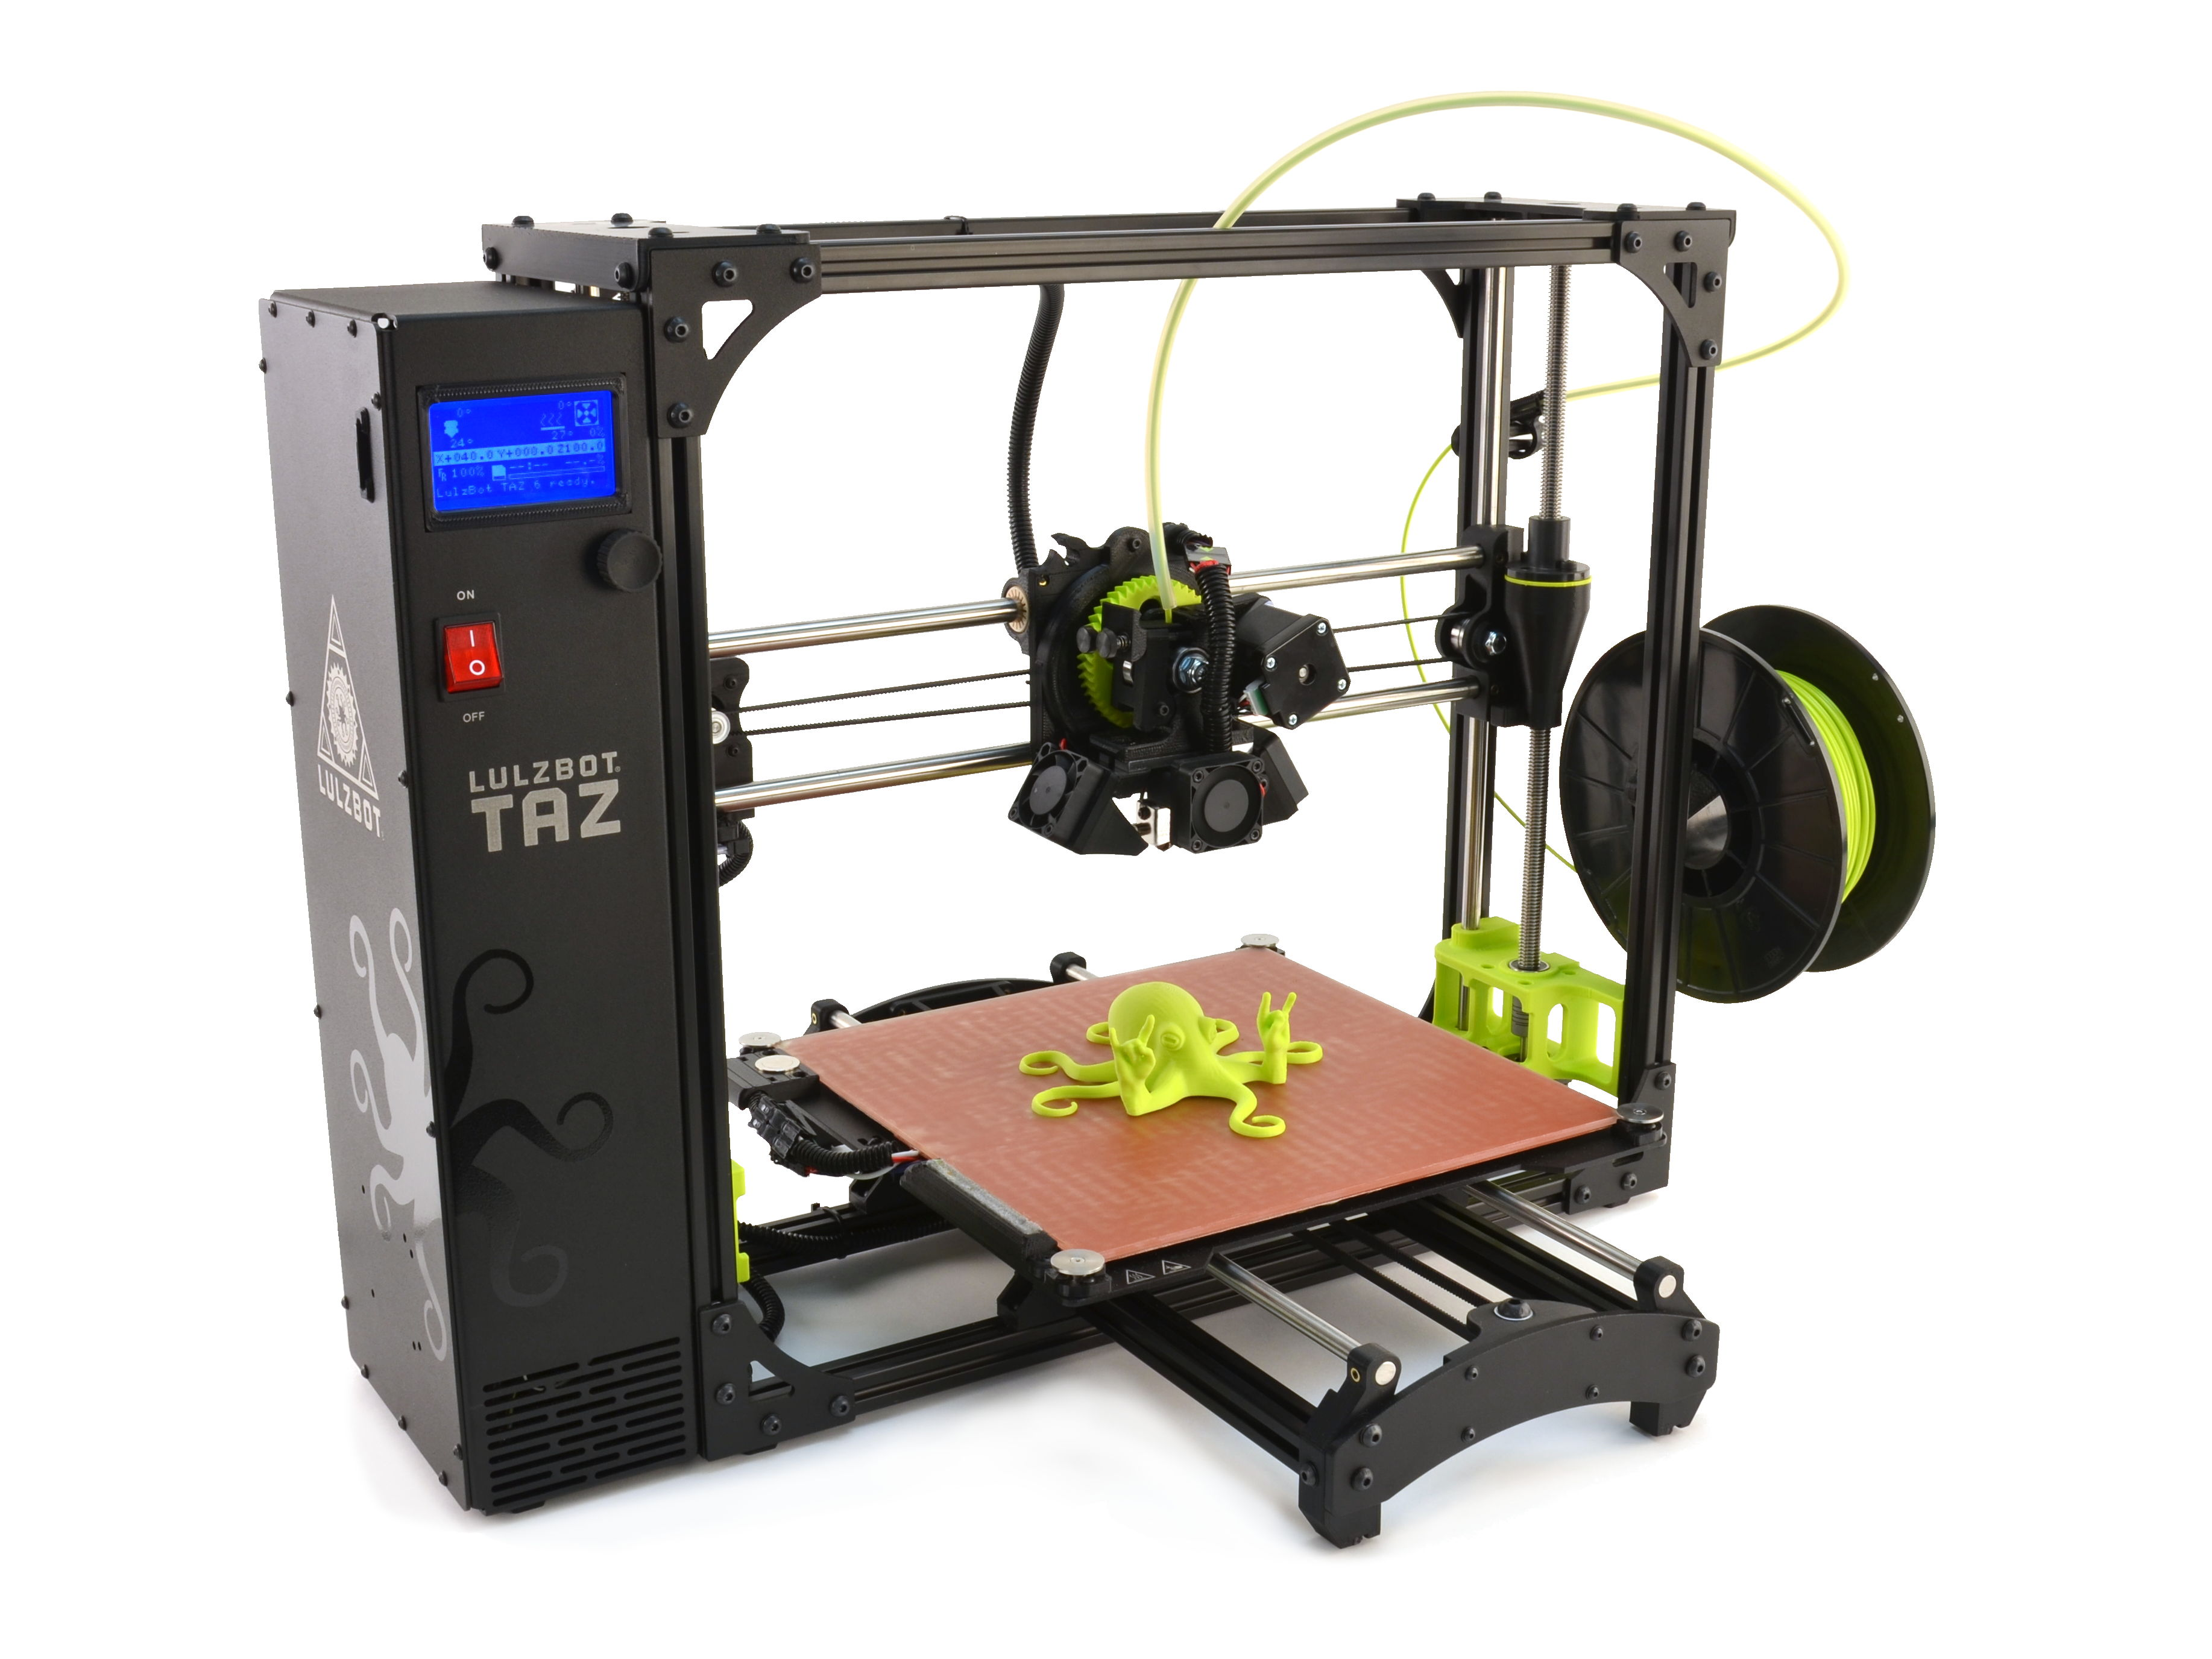
\includegraphics[keepaspectratio=true,angle=0,height=1.0\textheight,width=1.0\textwidth]{TAZ_6_Angle.JPG}

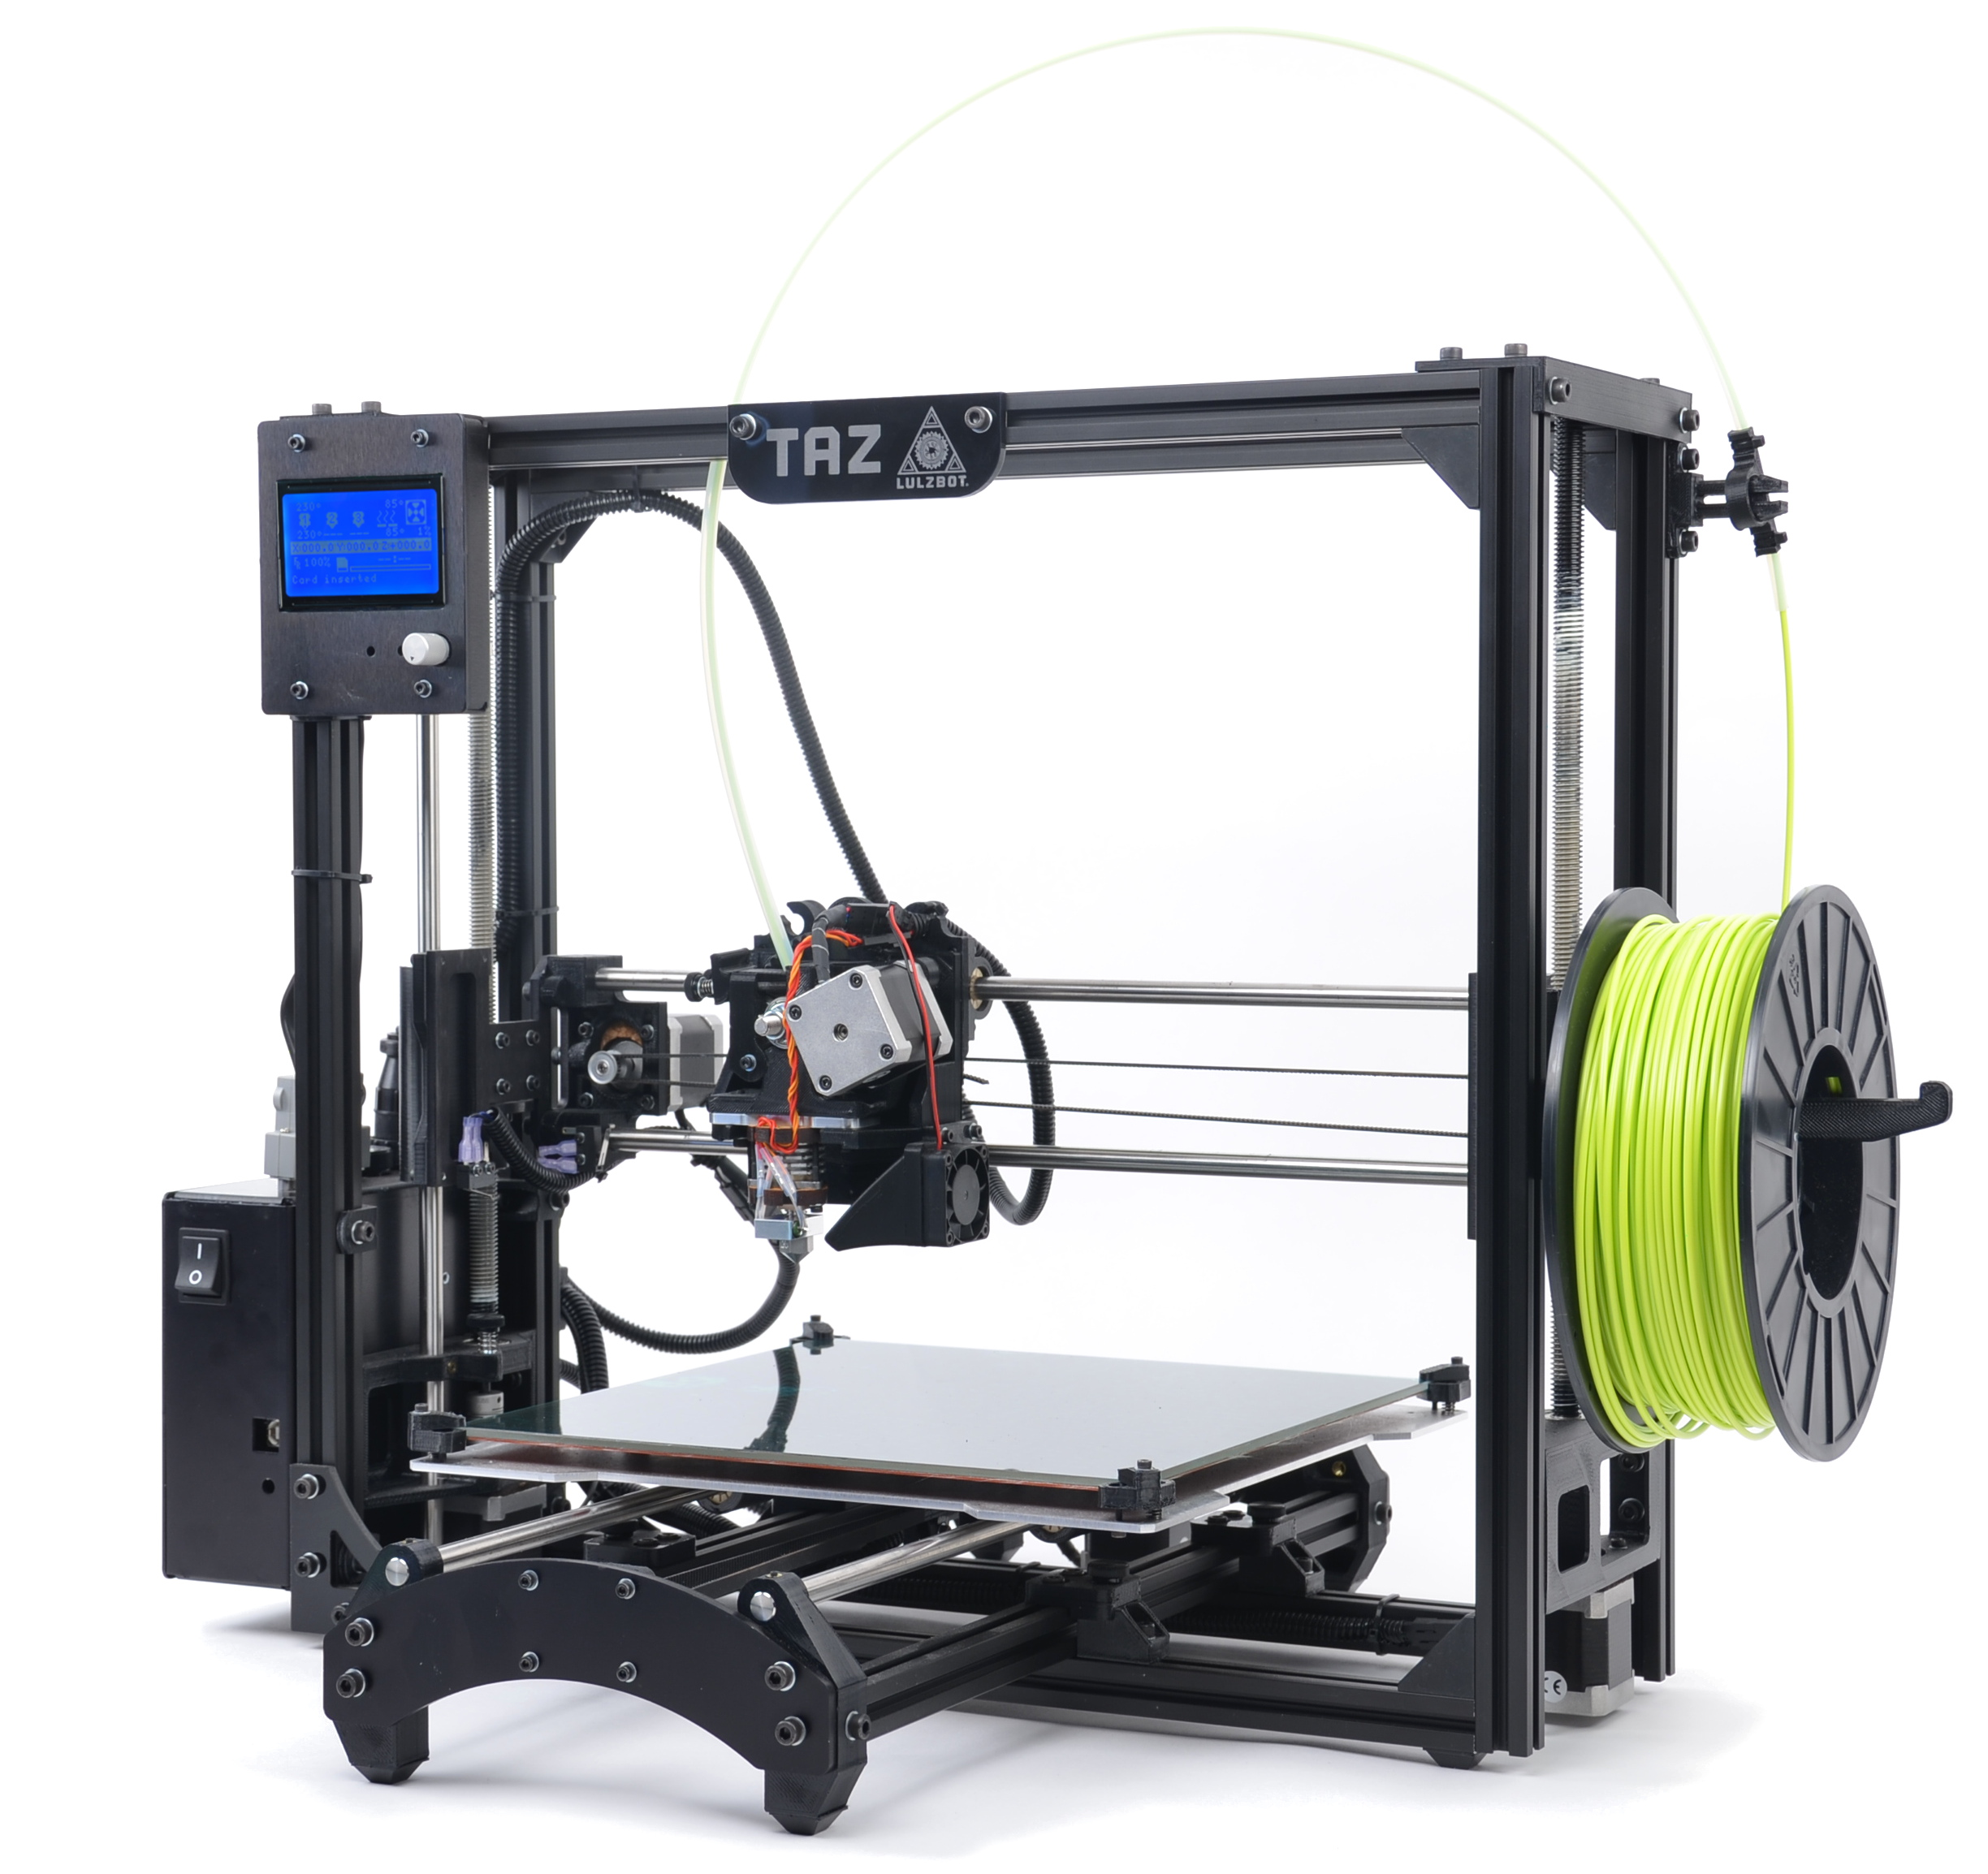
\includegraphics[keepaspectratio=true,angle=0,height=1.0\textheight,width=1.0\textwidth]{taz.jpg}


%\null\vfill
%\rule{0.4\textwidth}{0.4pt}
%\par
\begin{center}

\includegraphics[keepaspectratio=true,angle=0,height=0.25\textheight,width=0.25\textwidth]{Lulzbot_Logo_R_CMYK.eps}

{\large \itshape Aleph Objects, Inc.}
\end{center}
\endgroup
%\vspace*{0.1\textheight} 
%\newpage
%\clearpage
}
\fi
%%% END TITLE PAGE

%%% COPYRIGHT PAGE %%%
\ifcopyright
{\clearpage\null\vfill
\begingroup 
%\vfill\null 
\thispagestyle{empty}
\footnotesize\raggedright
\setlength{\parskip}{0.5\baselineskip}

\textbf{LulzBot\textsuperscript{\miniscule{\texttrademark}} TAZ 2.0 User Manual}

by Aleph Objects, Inc.

Copyright \copyright\ \the\year\ Aleph Objects, Inc.\par
Permission is granted to copy, distribute and\slash or modify 
this document under the terms of the
Creative Commons Attribution-ShareAlike 3.0 Unported license
(CC BY-SA 3.0).

Published by Aleph Objects, Inc., 123 SW 12th Street, Loveland, Colorado, 80537 USA.

For more information, call +1-970-377-1111 or go to \texttt{www.LulzBot.com} and \texttt{www.AlephObjects.com}.

ISBN: 978-0-9893784-2-0
\hfill\texttt{\the\year\the\month\the\day}
\endgroup
\pagebreak{}
}
\fi
%%% END COPYRIGHT PAGE %%%


%%% TABLE OF CONTENTS ToC %%%
\maxtocdepth{section}
% Dots
% space between dots
\renewcommand{\cftchapterdotsep}{15}
% dot symbol (default is period)
\renewcommand{\cftdot}{\textperiodcentered}	% centered period
% Set space between each entry in ToC
\setlength{\cftbeforechapterskip}{5pt}  % 5pt % 3pt
\tableofcontents*
%%% END TABLE OF CONTENTS ToC %%%

%%% LIST OF FIGURES %%%
%\addtodef{\listoffigures}{\clearpage\pagestyle{lof}}{}
% Fit all of List of Figures on one page
\renewcommand*{\lofheadstart}{\vspace{1cm}}
\clearpage
\listoffigures*
%%% END LIST OF FIGURES %%%

%%% CHAPTER STYLE %%%
\chapterstyle{jebinski} % defined in preamble
\def\topblockvspace{0.11}


%%% WARNINGS %%%
\ifwarnings
\chapter{\emph{WARNINGS}\protect \\
{Safety Information}}
\thispagestyle{empty}
\markboth{WARNING!}{Be Safe!}
{%
% Warnings.tex
%
% LulzBot® TAZ User Manual
%
% Copyright (C) 2014 Aleph Objects, Inc.
%
% This document is licensed under the Creative Commons Attribution 4.0
% International Public License (CC BY-SA 4.0) by Aleph Objects, Inc.
%

\section{\texttt{Read Me First!}}
\index{warnings}
\index{hazards}
\textcolor{red}{READ THIS MANUAL COMPLETELY BEFORE UNPACKING AND POWERING UP YOUR PRINTER.}

\section{\texttt{Hazards and Warnings}}

Your LulzBot\textsuperscript{\miniscule{\textregistered}} TAZ 3D printer has motorized and heated parts.  Always be aware of possible hazards when the printer is operational.


\subsection{\textcolor{red}{Electric Shock Hazard}}
\index{electronics}
\index{wires}
\index{power supply}
Never open the electronics case when the printer is powered on. Before removing the electronics case cover always power down the printer and completely turn off and unplug the power supply. Allow the power supply to discharge for at least one minute.

\subsection{\textcolor{red}{Burn Hazard}}
\index{extruder}
\index{heater block}
\index{temperature}
\index{burns}
Never touch the extruder nozzle or heater block without first turning off the hot end and allowing it to completely cool down. The hot end can take up to 20 minutes to completely cool. Never touch recently extruded plastic. The plastic can stick to your skin and cause burns. The heated bed can reach high temperatures that are capable of causing burns.

\subsection{\textcolor{red}{Fire Hazard}}
Never place flammable materials or liquids on or near the printer when it is powered on or operational. Liquid acetone and vapors are extremely flammable.

\subsection{\textcolor{red}{Pinch Hazard}}

When the printer is operational take care to never put your fingers in any moving parts including belts, pulleys, or gears. Tie back long hair or clothing that can get caught in the moving parts of the printer.

\subsection{\textcolor{red}{Static Charge}}
\index{static}
Make sure to ground yourself before touching the printer, especially its electronics. Electrostatic discharge can damage electronic components. Ground yourself by touching a grounded source like your computer case.

\subsection{\textcolor{red}{Age Warning}}

For users under the age of 18, adult supervision is recommended. Beware of choking hazards around small children.

\subsection{\textcolor{red}{Modifications and Repairs Warning}}

At Aleph Objects, Inc.\textsuperscript{\miniscule{\textregistered}} we respect your freedom to modify your LulzBot\textsuperscript{\miniscule{\textregistered}} desktop 3D printer. However any modifications or attempted repairs that cause damage are not covered under the Warranty. Questions? Contact Technical Support by emailing support@lulzbot.com, or by calling +1-970-377-1111.

\subsection{\texttt{Federal Communications Commission Statement}}
\index{FCC}
Note: This equipment has been tested and found to comply with the limits for a Class A digital device, pursuant to part 15 of the FCC Rules. These limits are designed to provide reasonable protection against harmful interference when the equipment is operated in a commercial environment. This equipment generates, uses, and can radiate radio frequency energy and, if not installed and used in accordance with the instruction manual, may cause harmful interference to radio communications. Operation of this equipment in a residential area is likely to cause harmful interference in which case the user will be required to correct the interference at his own expense.

This device complies with part 15 class A of the FCC Rules. Operation is subject to the following two conditions:
\begin{enumerate}
\item This device may not cause harmful interference and
\item This device must accept any interference received, including interference that may cause undesired operation.
\end{enumerate}

\textcolor{red}{FCC Warning:}
\textcolor{red}{Changes or modifications not approved by the party responsible for compliance could void the users authority to operate the equipment.}



}
\fi
%%% END WARNINGS %%%

%%% END FRONTMATTER %%%
%%% BEGIN MAINMATTER %%%
\mainmatter*

% Set page numbering to arabic, but don't reset numbering (*)
\pagenumbering*{arabic}

%%% SETUP %%%
\ifsetup
\chapter{\emph{Setup Your Printer}}
\thispagestyle{empty}
\markboth{Setup Your Printer}{LulzBot TAZ User Manual}
{\begin{enumerate}
\item Your printer has been pre-calibrated and tested; however, after unpacking all of the components you will need to re-mount the Y axis onto the frame and connect the bed and Y axis connectors. You will also need to re-mount the extruder toolhead. Please follow the steps completely to make certain that the extruder toolhead and Y axis are re-mounted correctly and you will be on your way to your first print.

\item Place the TAZ frame and Y axis assembly on a flat and level surface. Move to the Y axis assembly and find the four Y axis bolts. The four bolts, located on the Y axis aluminum frame bars, have large plastic knobs that allow the bolts to be easily turned by hand (Fig. \ref{fig:Y_axis_bolts}, page \pageref{fig:Y_axis_bolts}). Turning counter clock-wise, remove each of the four Y axis bolts and set aside (Fig. \ref{fig:remove_Y_axis_bolts}, page \pageref{fig:remove_Y_axis_bolts}).

\begin{figure}[hp]
\centering
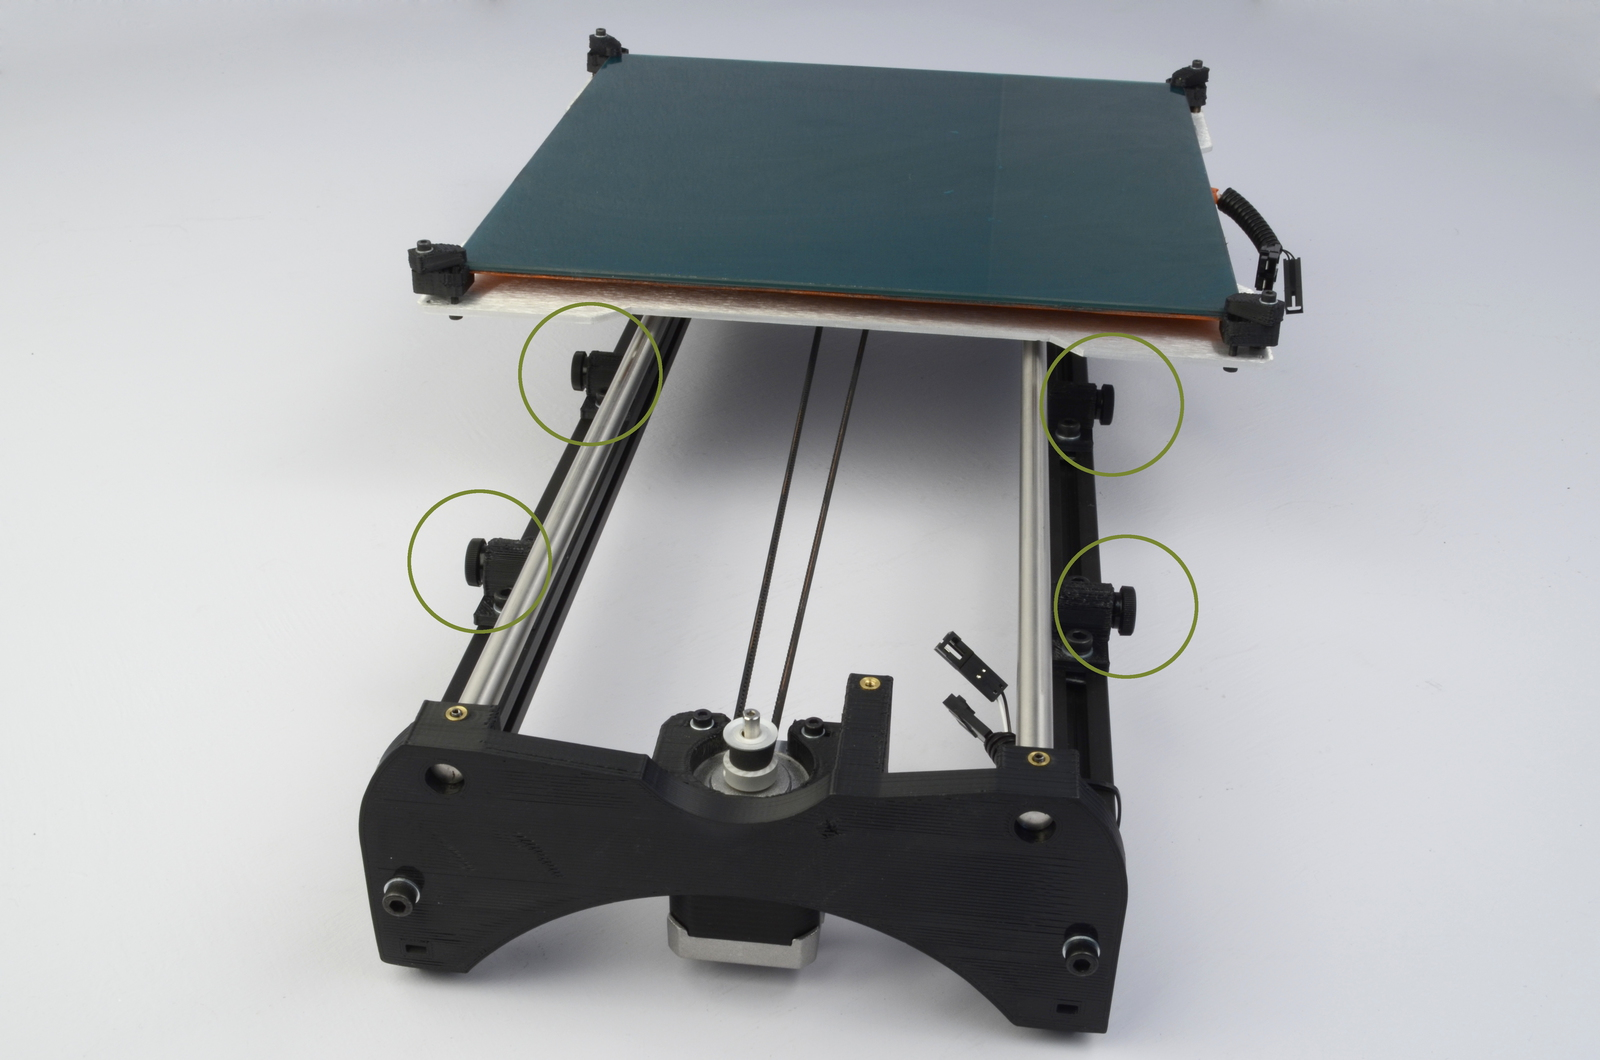
\includegraphics[keepaspectratio=true,angle=0,height=0.4\textheight,width=1.0\textwidth]{y_axis_bolts.JPG}
\caption{Locate the four Y axis bolts}
\label{fig:Y_axis_bolts}
\end{figure}

%\begin{figure}[hp] CD changed to force pic placement
\begin{figure}[H]
\centering
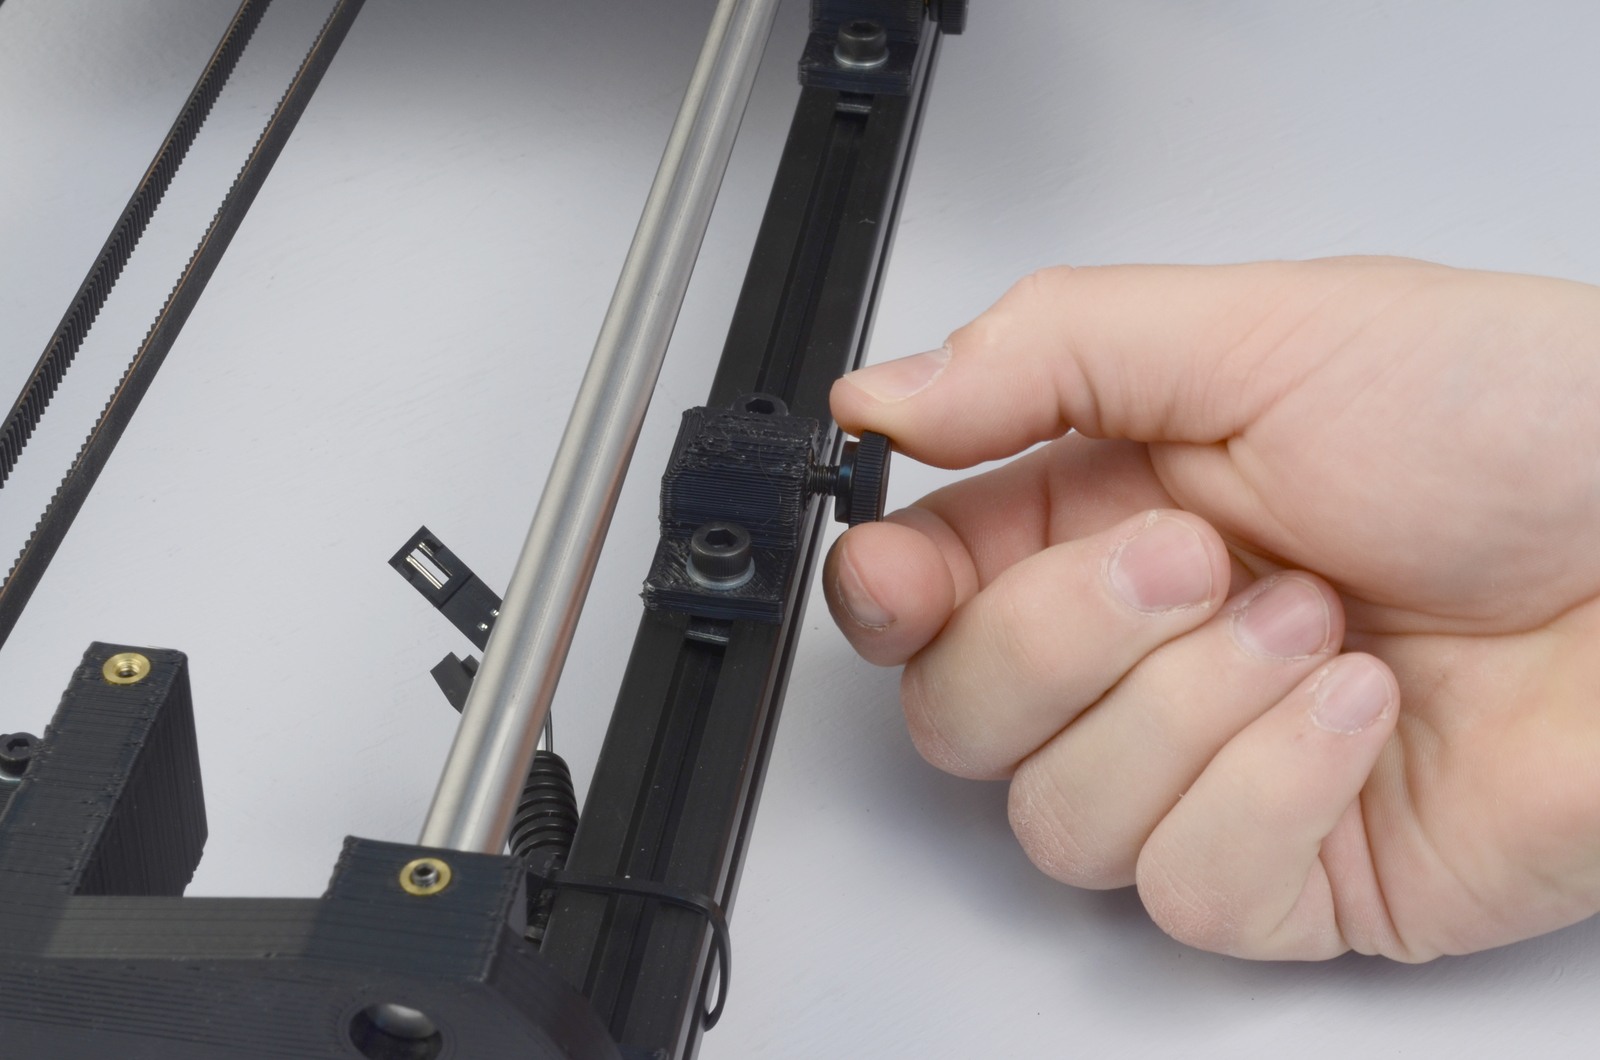
\includegraphics[keepaspectratio=true,angle=0,height=0.4\textheight,width=1.0\textwidth]{y_axis_bolt_remove.JPG}
\caption{Remove the four Y axis bolts}
\label{fig:remove_Y_axis_bolts}
\end{figure}

\item On the TAZ frame locate the four Y axis mount brackets shown in Fig. \ref{fig:frame_Y_axis_mounts} (pg. \pageref{fig:frame_Y_axis_mounts}). With the print surface facing up and the stepper motor end of the Y axis facing back, slide the Y axis assembly in between the Y axis mount brackets. The four Y axis mount brackets will line up with the Y axis bolt holes on the Y axis assembly. Thread the four Y axis bolts through the brackets, into the Y axis assembly (Fig. \ref{fig:Y_axis_bolts_tighten}, page \pageref{fig:Y_axis_bolts_tighten}). Before completely tightening the Y axis bolts make sure the Y axis aluminum bars are pushed down against the TAZ frame lower bars. You can do this by slightly tilting the printer, on the side edge, enough to lift the feet of the Y axis off of the table. The weight of the Y axis will seat it against the TAZ frame. While the printer is slightly tilted tighten the four Y axis bolts. The printer can be now be set flat on the table.
%\begin{figure}[hp] CD forcing image placement
\begin{figure}[H]
\centering
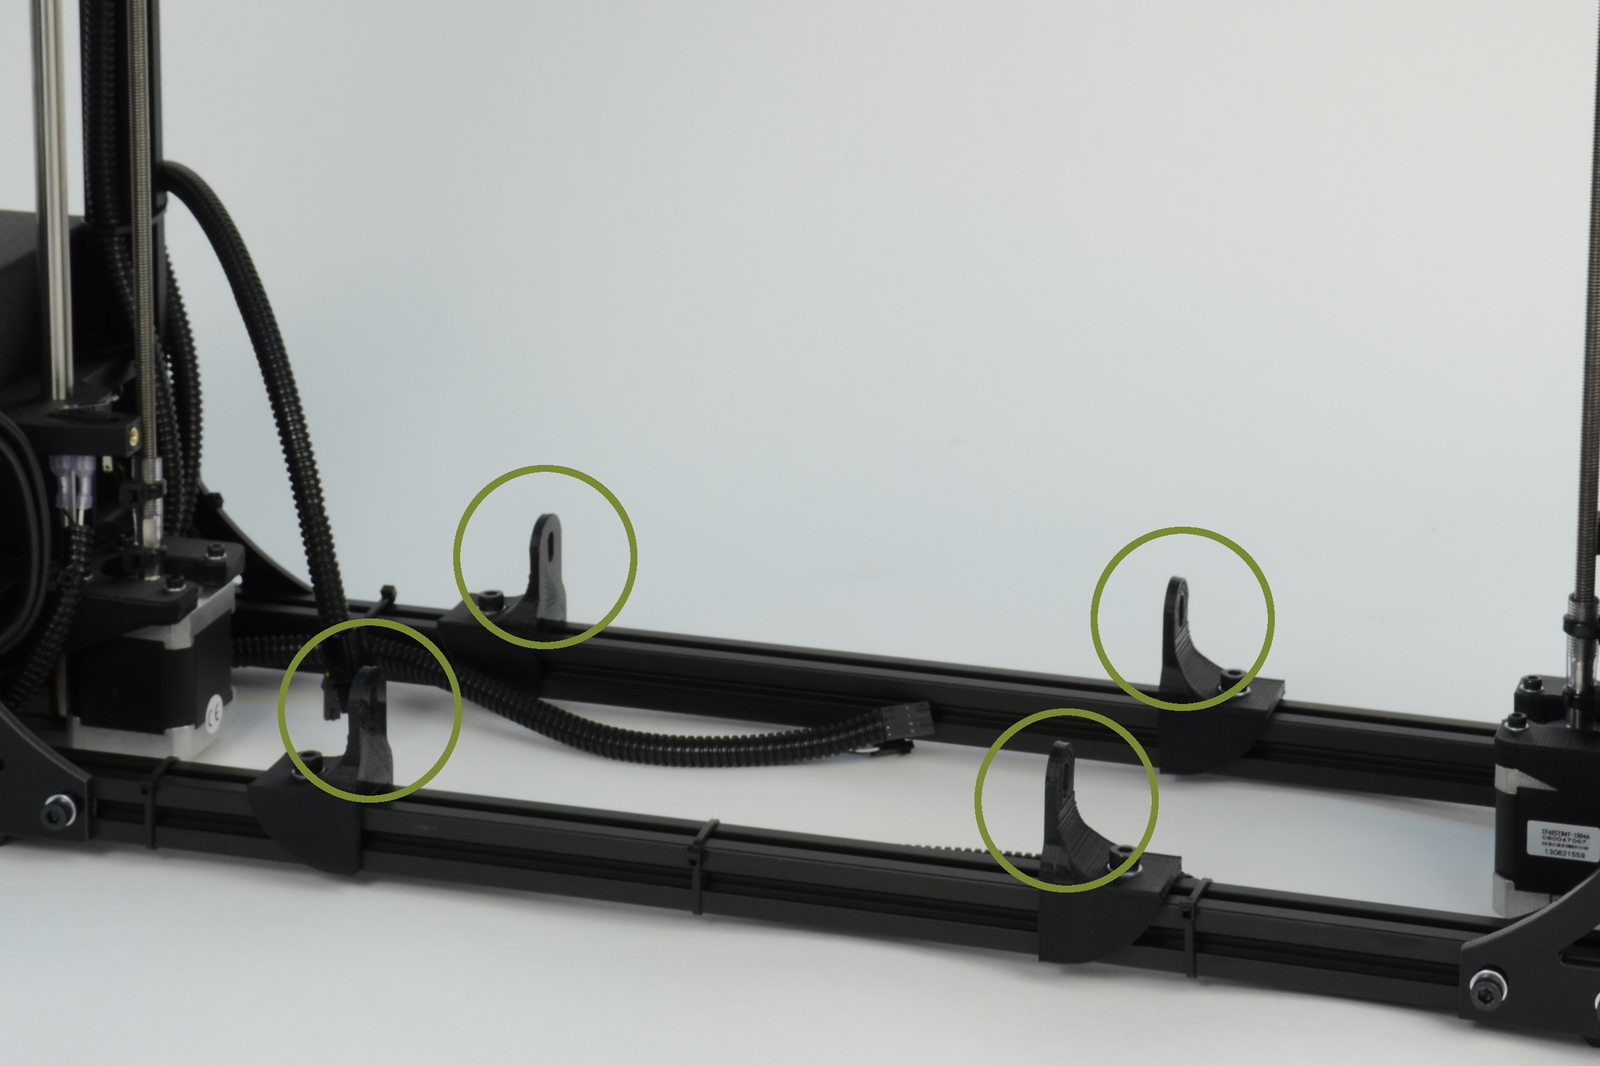
\includegraphics[keepaspectratio=true,angle=0,height=0.4\textheight,width=1.0\textwidth]{frame_y_axis_connector.JPG}
\caption{Locate the four Y axis mounts on the frame}
\label{fig:frame_Y_axis_mounts}
\end{figure}

%\begin{figure}[hp] CD forcing image placement
\begin{figure}[H]
\centering
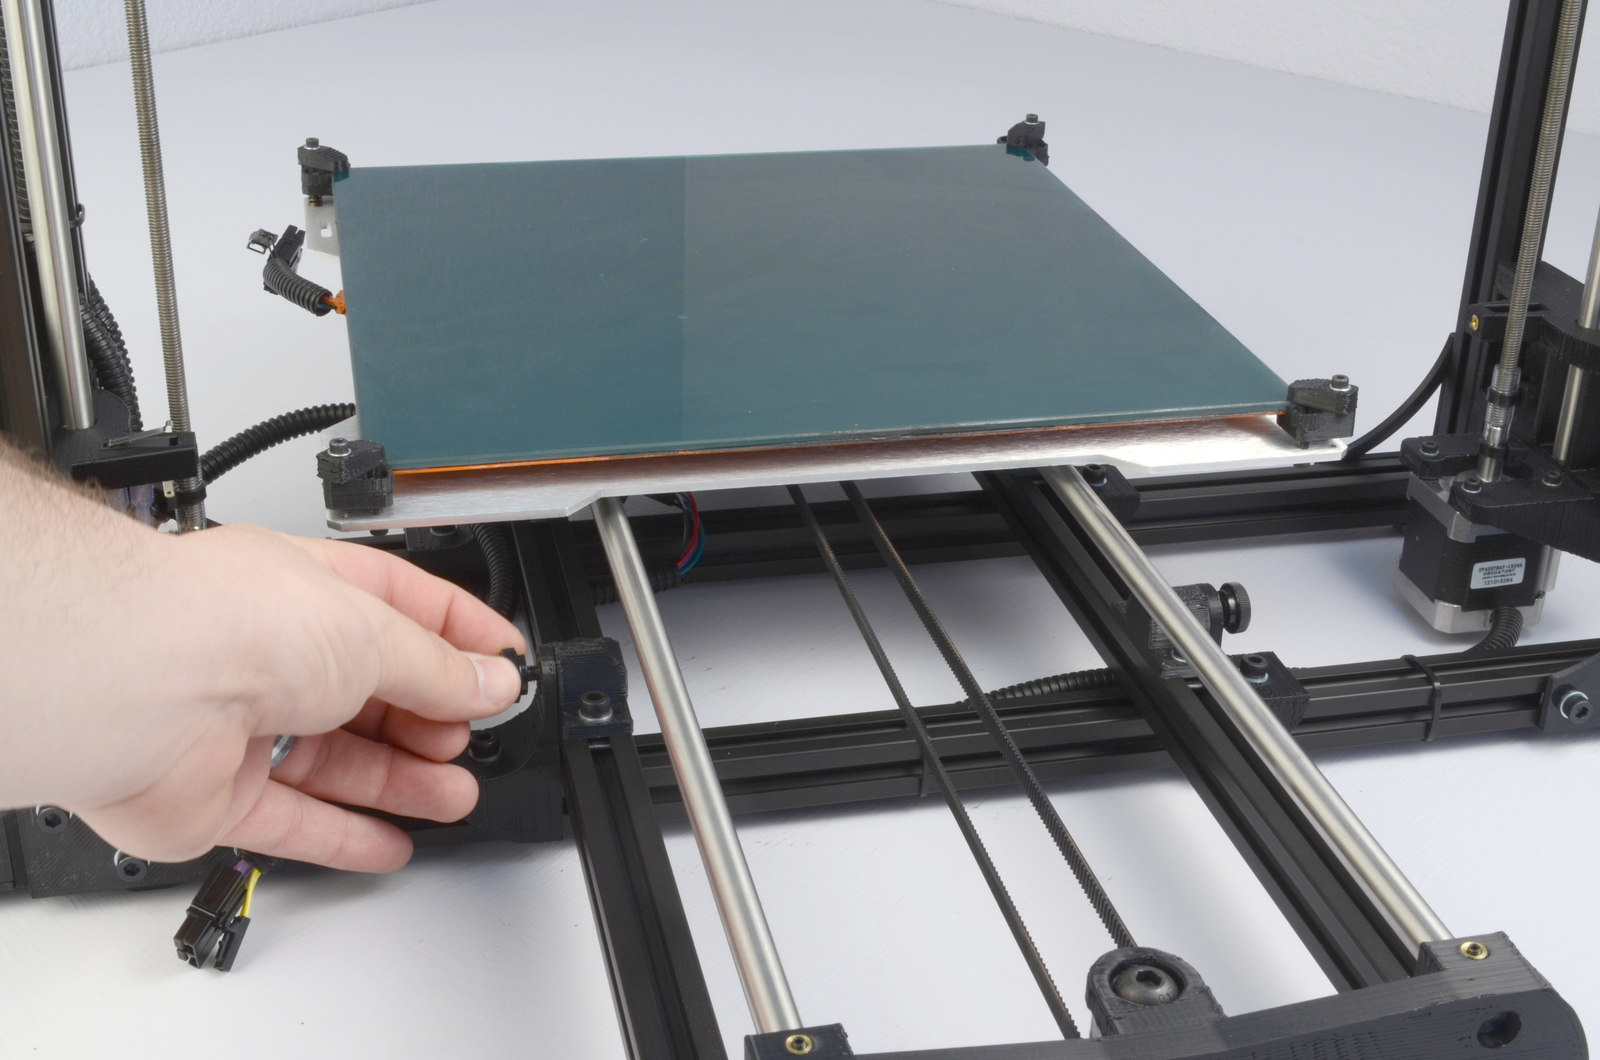
\includegraphics[keepaspectratio=true,angle=0,height=0.4\textheight,width=1.0\textwidth]{y_axis_bolt_tighten.JPG}
\caption{Screw in and tighten the four Y axis bolts}
\label{fig:Y_axis_bolts_tighten}
\end{figure}

\item The final step of installing the Y axis is connecting the print surface connectors and Y axis connectors. Pull the print bed completely to the front of the printer to get access to the Y axis connectors. You will find matching male and female 4 pin stepper motor connectors and two pin end stop connectors. Connect the matching male and female connectors (Fig. \ref{fig:Y_axis_connectors}, page \pageref{fig:Y_axis_connectors}); make sure the connector lock clicks to be sure that the connection is secure.


\begin{figure}[p]
\centering
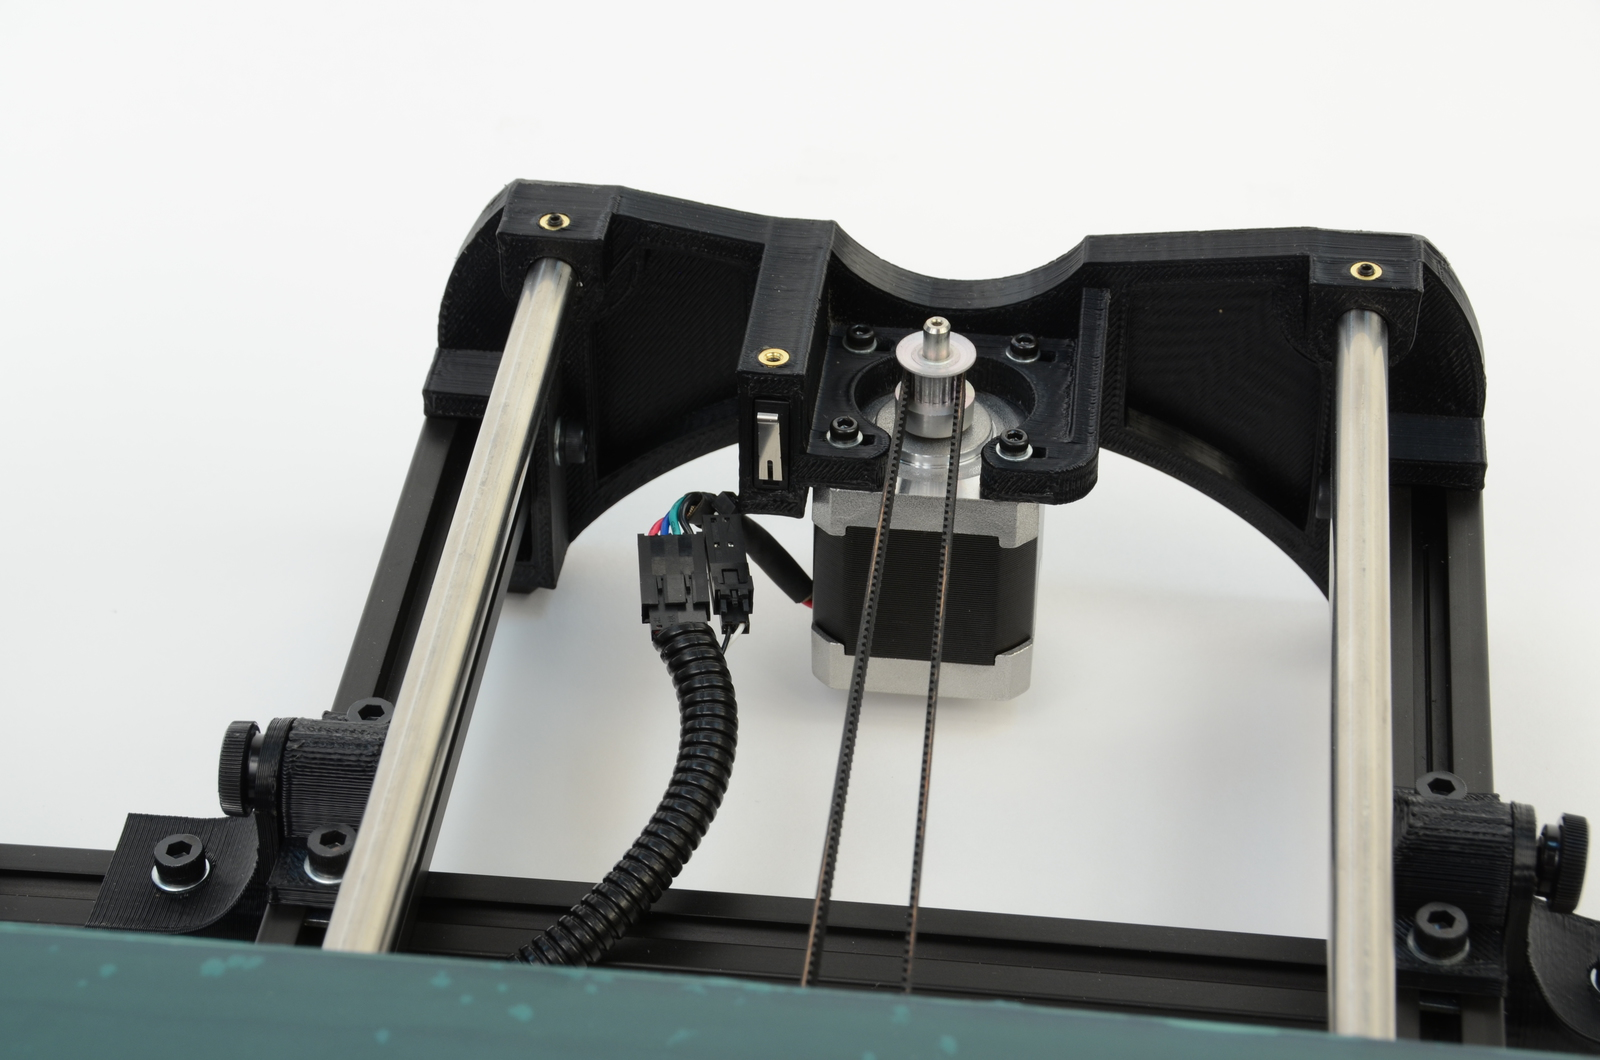
\includegraphics[keepaspectratio=true,angle=0,height=0.4\textheight,width=1.0\textwidth]{y_axis_connectors.JPG}
\caption{Connect the two connectors found at the rear of the Y axis}
\label{fig:Y_axis_connectors}
\end{figure}

\item Locate the two connectors to the left of the print bed. Connect the matching female and male large two pin heat bed connectors and the small two pin connectors (Fig. \ref{fig:bed_connectors}, page \pageref{fig:bed_connectors}).

\begin{figure}[p]
\centering
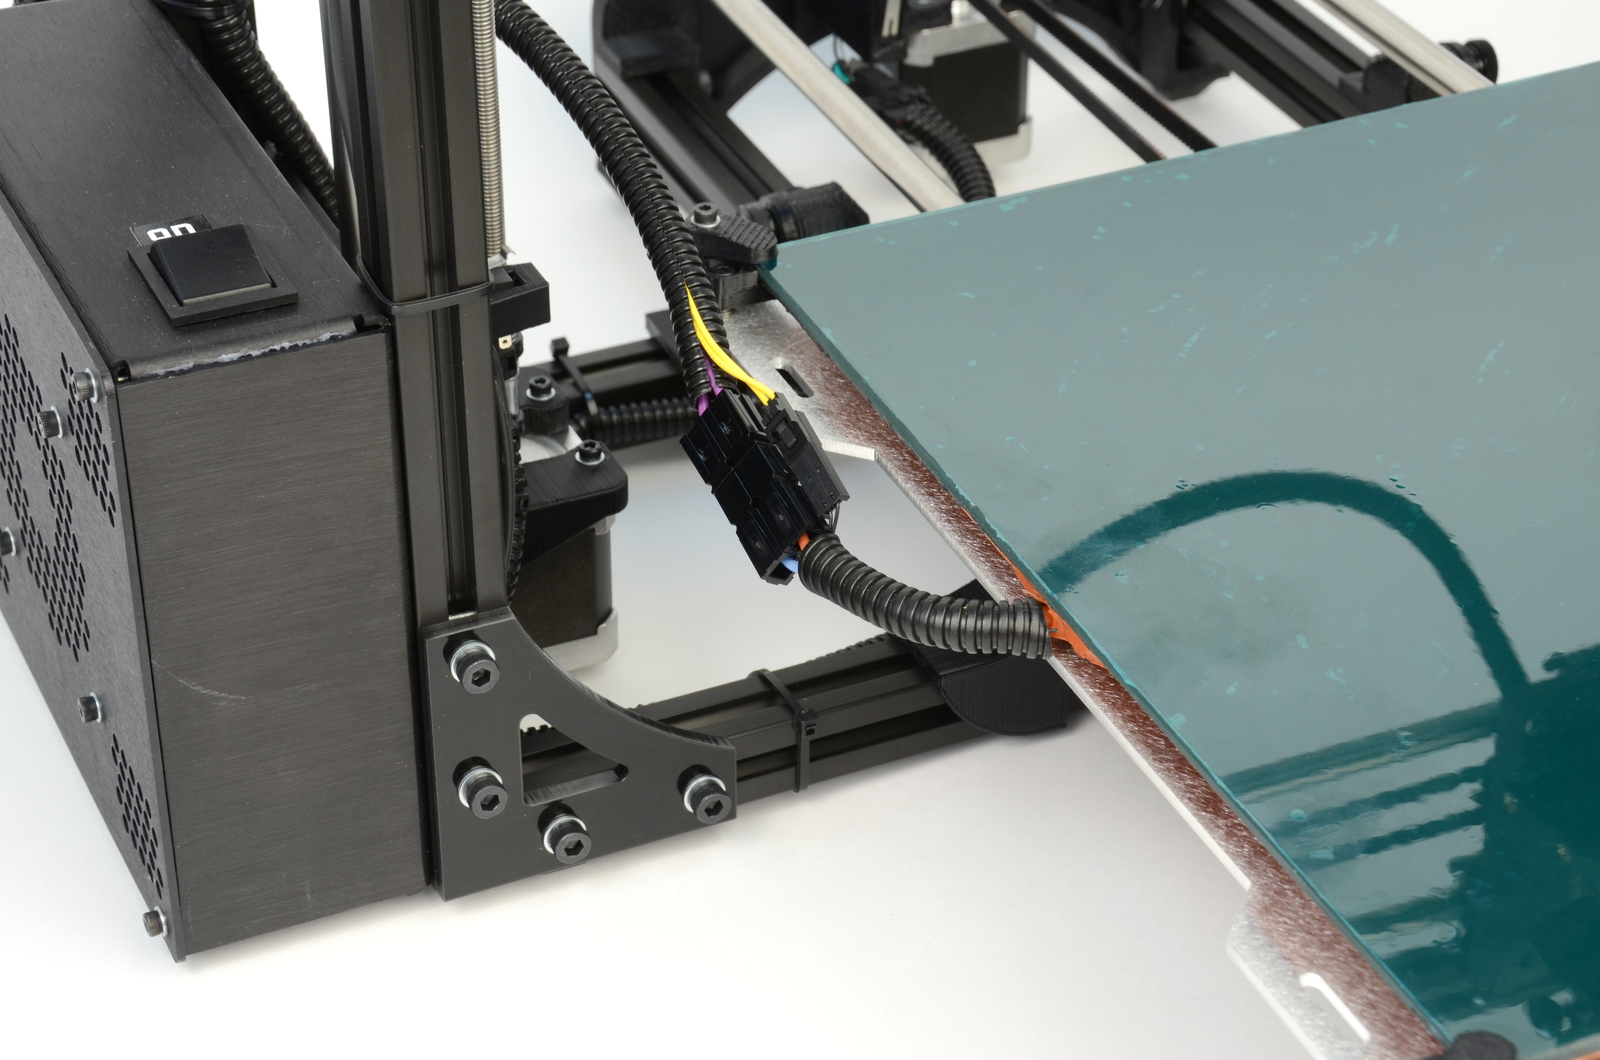
\includegraphics[keepaspectratio=true,angle=0,height=0.4\textheight,width=1.0\textwidth]{bed_connectors.JPG}
\caption{Connect the two connectors on the left of the print bed}
\label{fig:bed_connectors}
\end{figure}

\item Locate the two small black zip ties that are included in the documents bag (Fig. \ref{fig:bed_connectors_strain_relief}, page \pageref{fig:bed_connectors_strain_relief}). Wrap the two zip ties through the slot, located on the left rear of the aluminum bed plate, and around the print bed wires (Fig. \ref{fig:bed_connectors_strain_relief_done}, page \pageref{fig:bed_connectors_strain_relief_done}). Tighten the zip ties snug so the wire cannot move freely. Cut off the excess end of the zip ties with the needle nose pliers included in the tool bag.

%\begin{figure}[hp] CD forcing image placement
\begin{figure}[H]
\centering
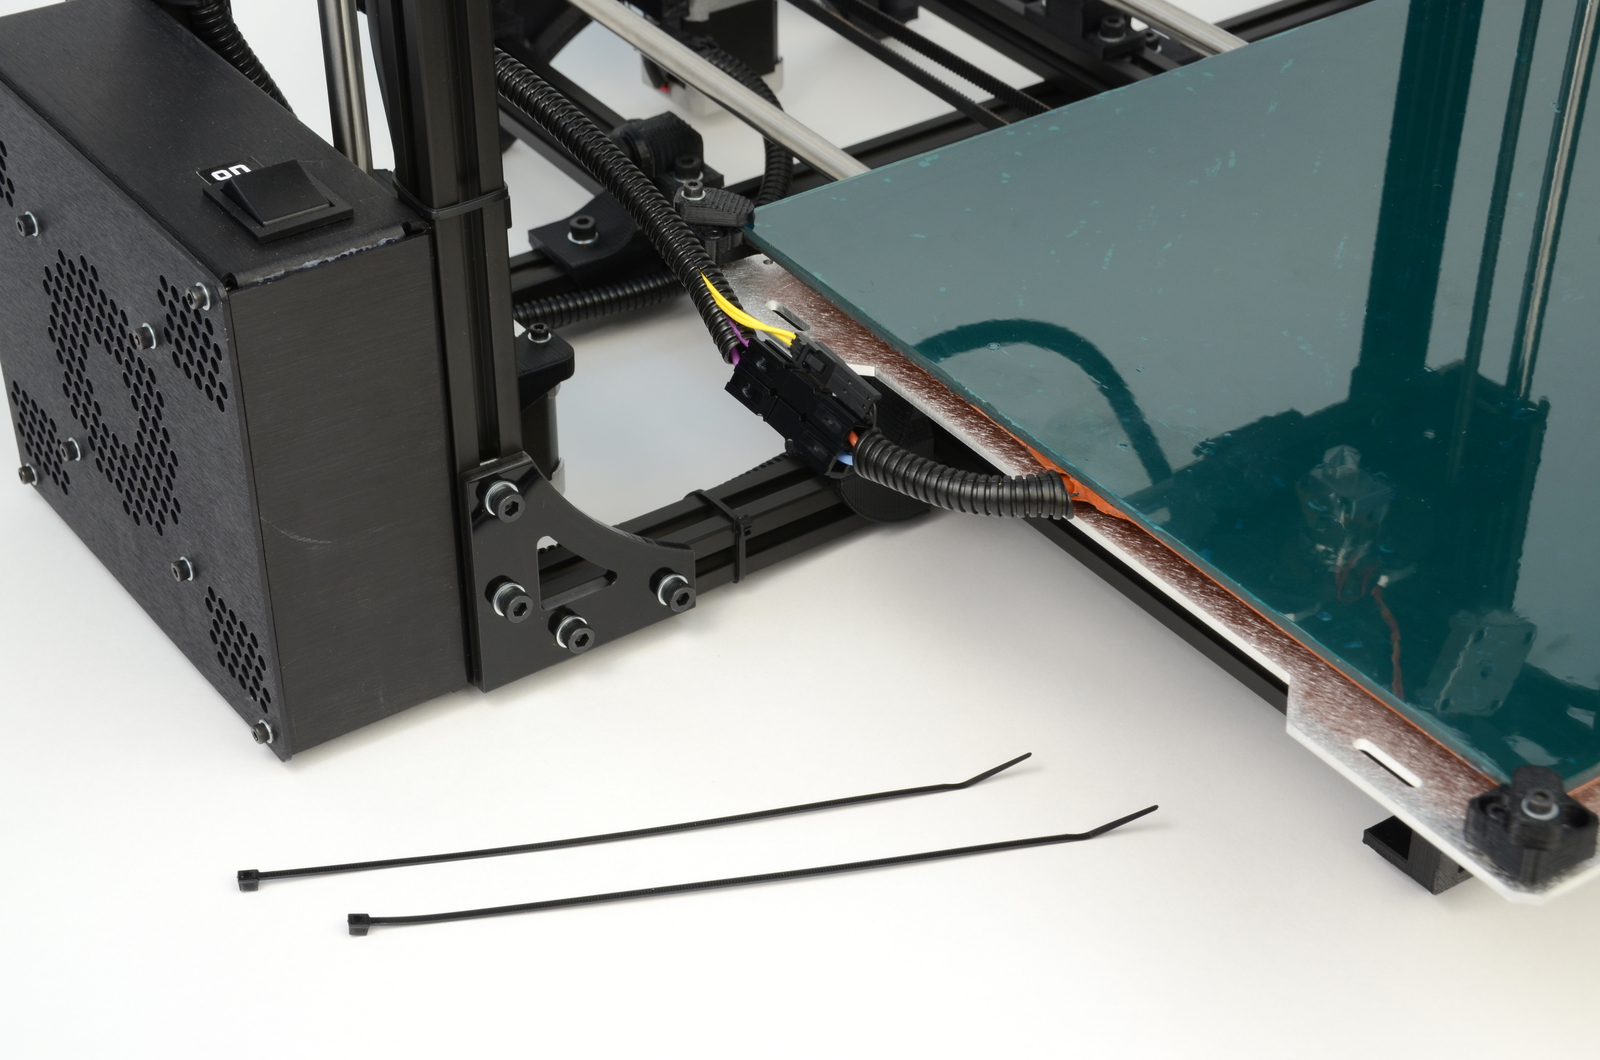
\includegraphics[keepaspectratio=true,angle=0,height=0.4\textheight,width=1.0\textwidth]{bed_connectors_strain_relief.JPG}
\caption{Locate the two zip ties found in the bag with the manual}
\label{fig:bed_connectors_strain_relief}
\end{figure}

%\begin{figure}[hp] CD forcing image placement
\begin{figure}[H]
\centering
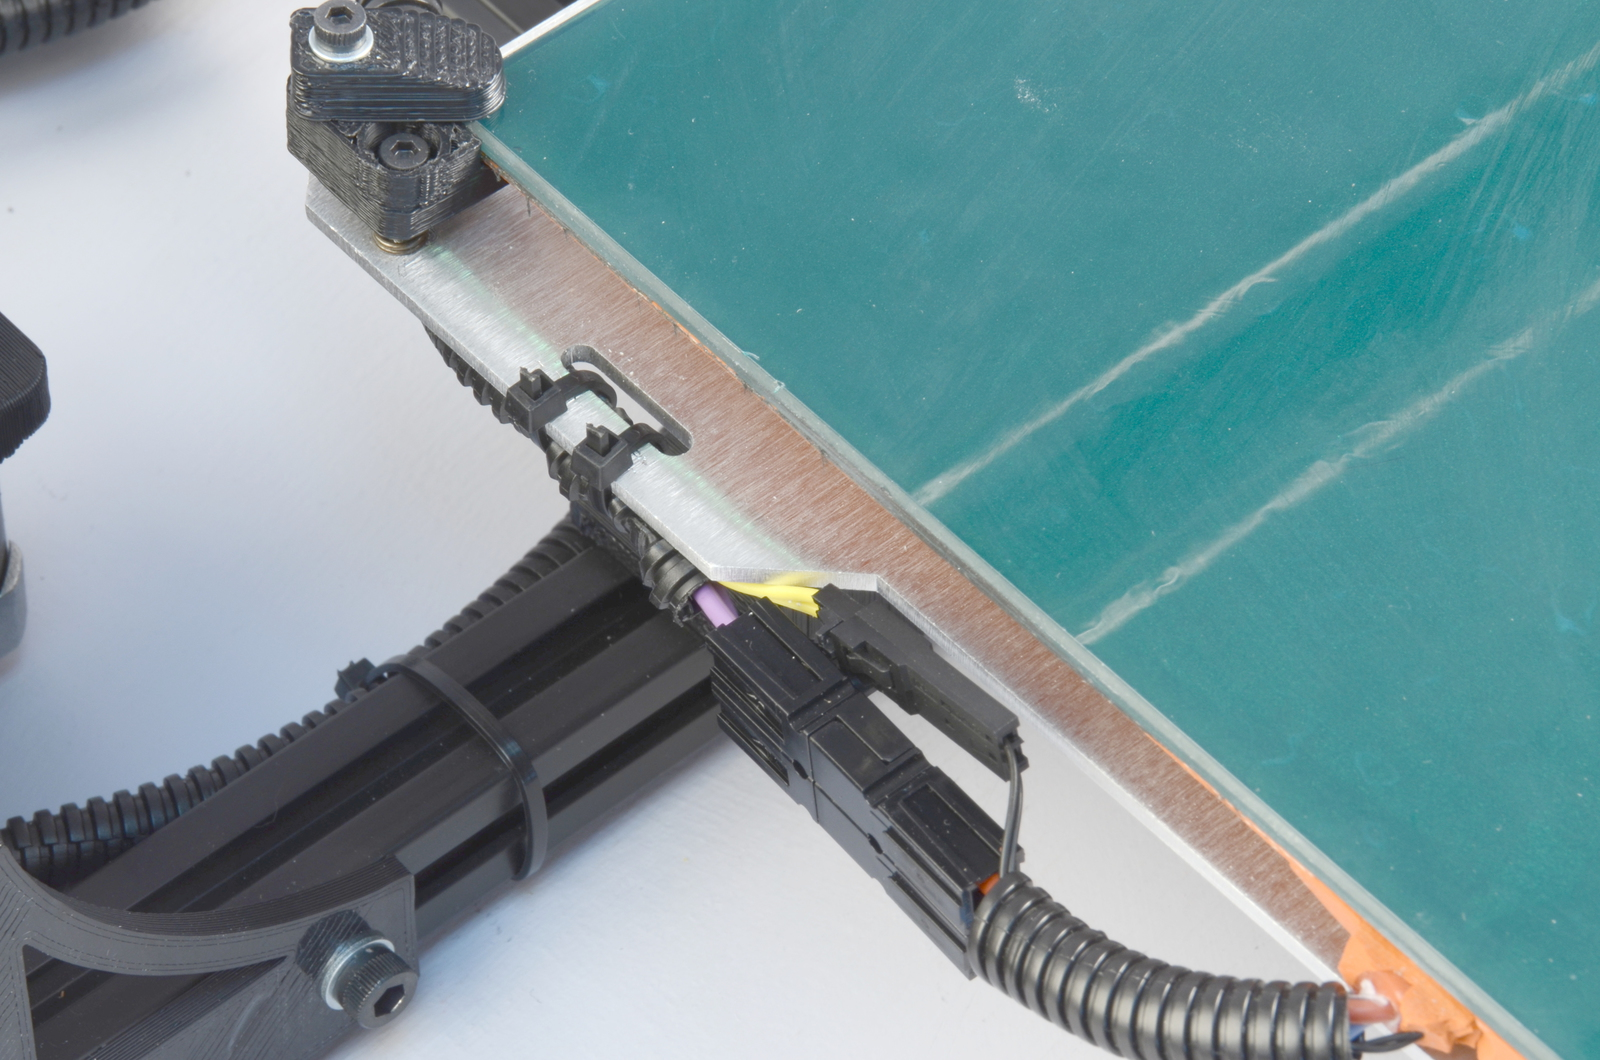
\includegraphics[keepaspectratio=true,angle=0,height=0.4\textheight,width=1.0\textwidth]{bed_connectors_strain_relief_done.JPG}
\caption{Tightly wrap the zip ties around the bed wires and through the strain relief slot}
\label{fig:bed_connectors_strain_relief_done}
\end{figure}

\item Move the X axis carriage over to the center of the smooth rods. Remove the foam from between the X axis carriage and the X axis ends. Locate the extruder toolhead screw from the accessories bag and place the extruder toolhead onto the X axis carriage. The extruder mount will slide into the bottom portion of the carriage and self center. Use the included 2.5mm driver to secure the extruder tool head onto the X axis carriage.
\begin{figure}[hp]
\centering
\includegraphics[keepaspectratio=true,angle=0,height=0.4\textheight,width=1.0\textwidth]{PIC_of_extruder mount installation.JPG}
\caption{Mount the extruder tool head}
\label{fig:PIC-of-initial-position}
\end{figure}

\item Connect the stepper motor and the hot end to the existing wiring harness. The connections are keyed and can only be connected in the correct orientation.
\begin{figure}[hp]
\centering
\includegraphics[keepaspectratio=true,angle=0,height=0.4\textheight,width=1.0\textwidth]{PIC_of_extruder_connections.JPG}
\caption{Extruder connections}
\label{fig:PIC_of_extruder_connections}
\end{figure}

\item Secure the wiring harness into the strain relief on the top left hand side of the X axis carriage. 
\begin{figure}[hp]
\centering
\includegraphics[keepaspectratio=true,angle=0,height=0.4\textheight,width=1.0\textwidth]{PIC_of_strain_relief.JPG}
\caption{Strain relief installation}
\label{fig:PIC_of_strain_relief}
\end{figure}

\item Now that the Y axis is mounted and the extruder tool head is installed you should set your printer on a stable, flat, and level surface large enough for extra space around the printer. Make sure your printer work space is clear of anything that could obstruct the movement of the printer. \textcolor{red}{Make sure there are no flammable fabrics or liquids near the printer space}. It is also best to not put your printer near a drafty window or air conditioner vent.

\index{power supply}
\index{USB cable}
\item Unwrap the power supply and USB cables.

\textcolor{red}{MAKE SURE THE POWER SUPPLY IS COMPLETELY UNPLUGGED BEFORE MOVING ON TO THE NEXT STEP}.

\index{electronics receptacles}
\item Locate the power supply and USB receptacles along the back of the TAZ electronics enclosure
(Fig. \ref{fig:electronics_plugs}, page \pageref{fig:electronics_plugs}). Locate the power supply and the included AC power cable (Fig. \ref{fig:power_supply}, page \pageref{fig:power_supply}). Locate the DC power cable plug on the power supply. Connect the DC locking plug into the DC connector on the TAZ electronics enclosure (Fig. \ref{fig:ps_plug}, page \pageref{fig:ps_plug}). The plug is keyed which may require rotating the plug until the keys line up and the plug can be pushed in. Once you have pushed in the plug turn the locking sleeve clockwise until it is tight against the electronics enclosure (Fig. \ref{fig:electronics_plugs_plugged-in}, page \pageref{fig:electronics_plugs_plugged-in}).
%\begin{figure}[hbt]
\begin{figure}[H]
\centering
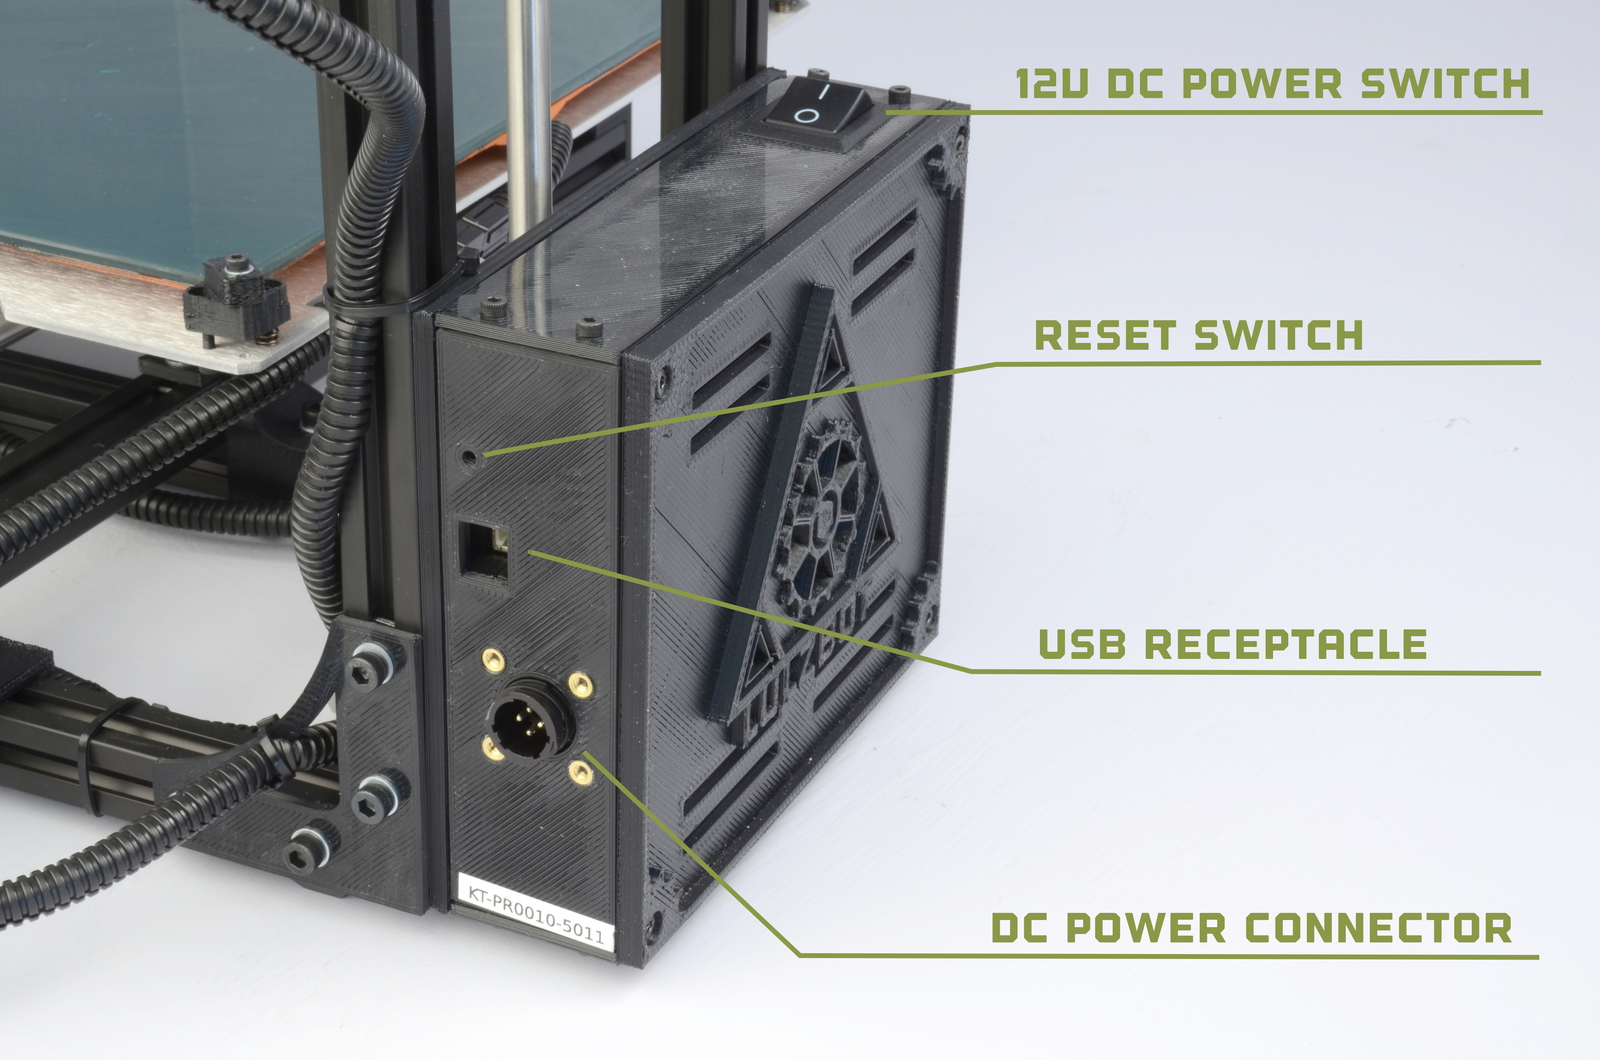
\includegraphics[keepaspectratio=true,angle=0,height=0.4\textheight,width=1.0\textwidth]{electronics_case_rec.JPG}
\caption{Power supply and USB receptacles}
\label{fig:electronics_plugs}
\end{figure}

%\begin{figure}[hp]
\begin{figure}[H]
\centering
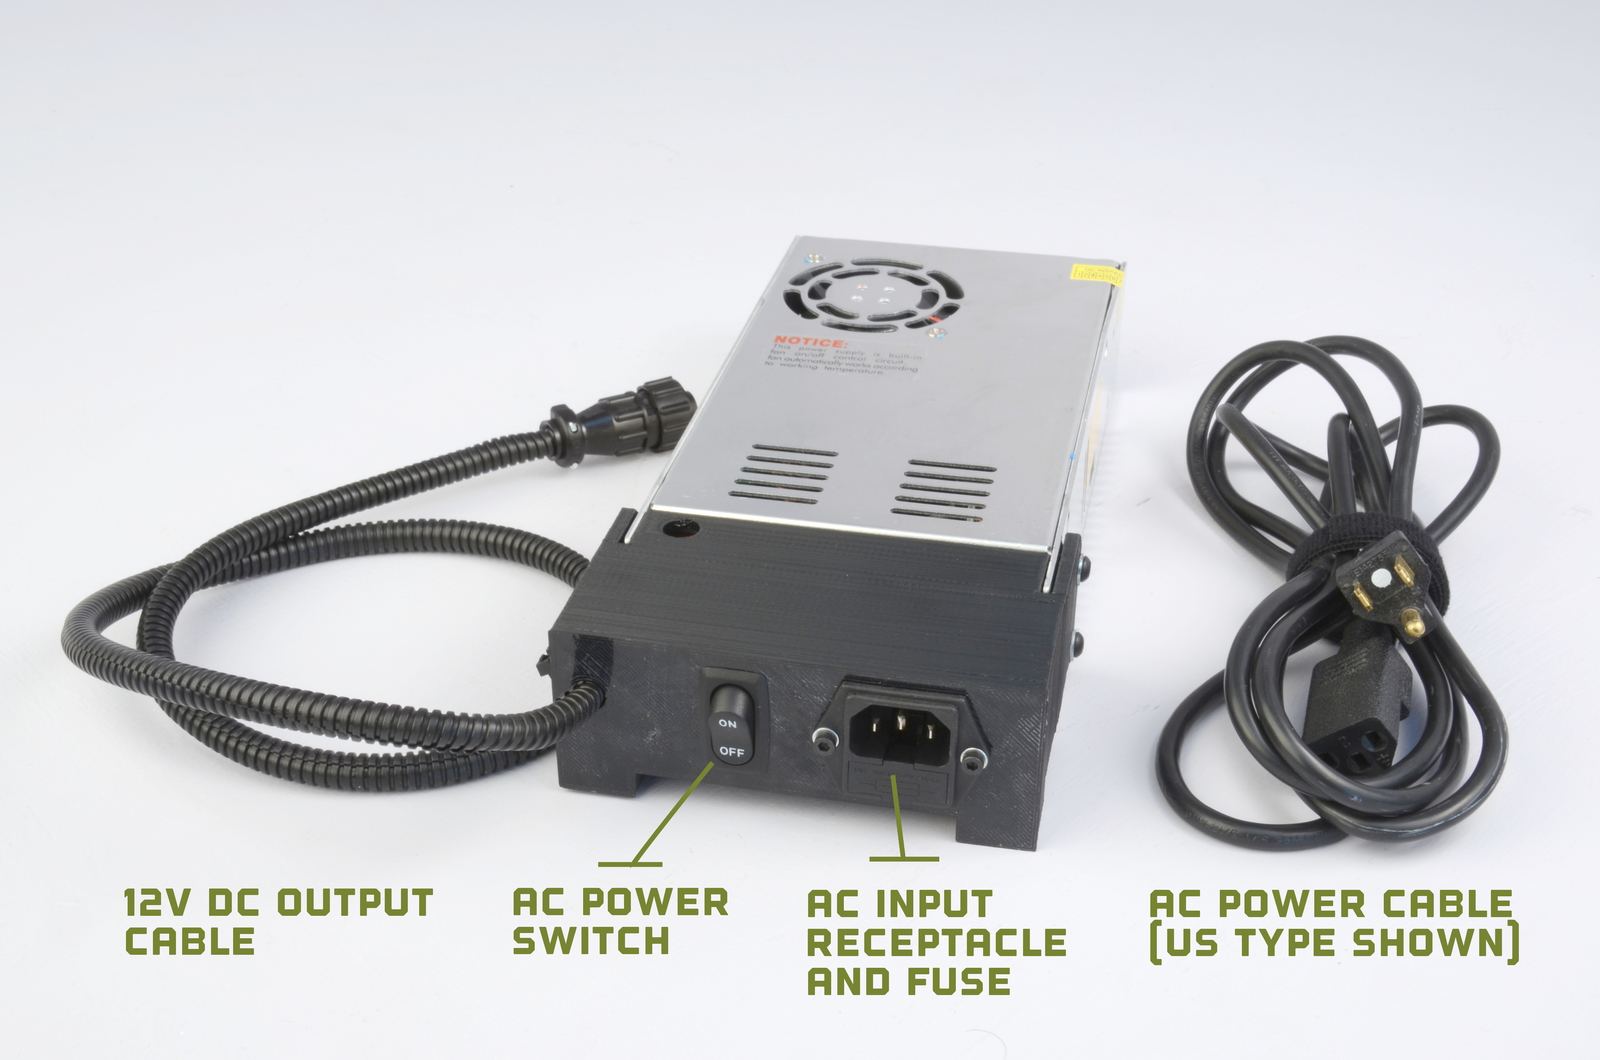
\includegraphics[keepaspectratio=true,angle=0,height=0.4\textheight,width=1.0\textwidth]{power_supply.JPG}
\caption{Power supply}
\label{fig:power_supply}
\end{figure}

%\begin{figure}[hp]
\begin{figure}[H]
\centering
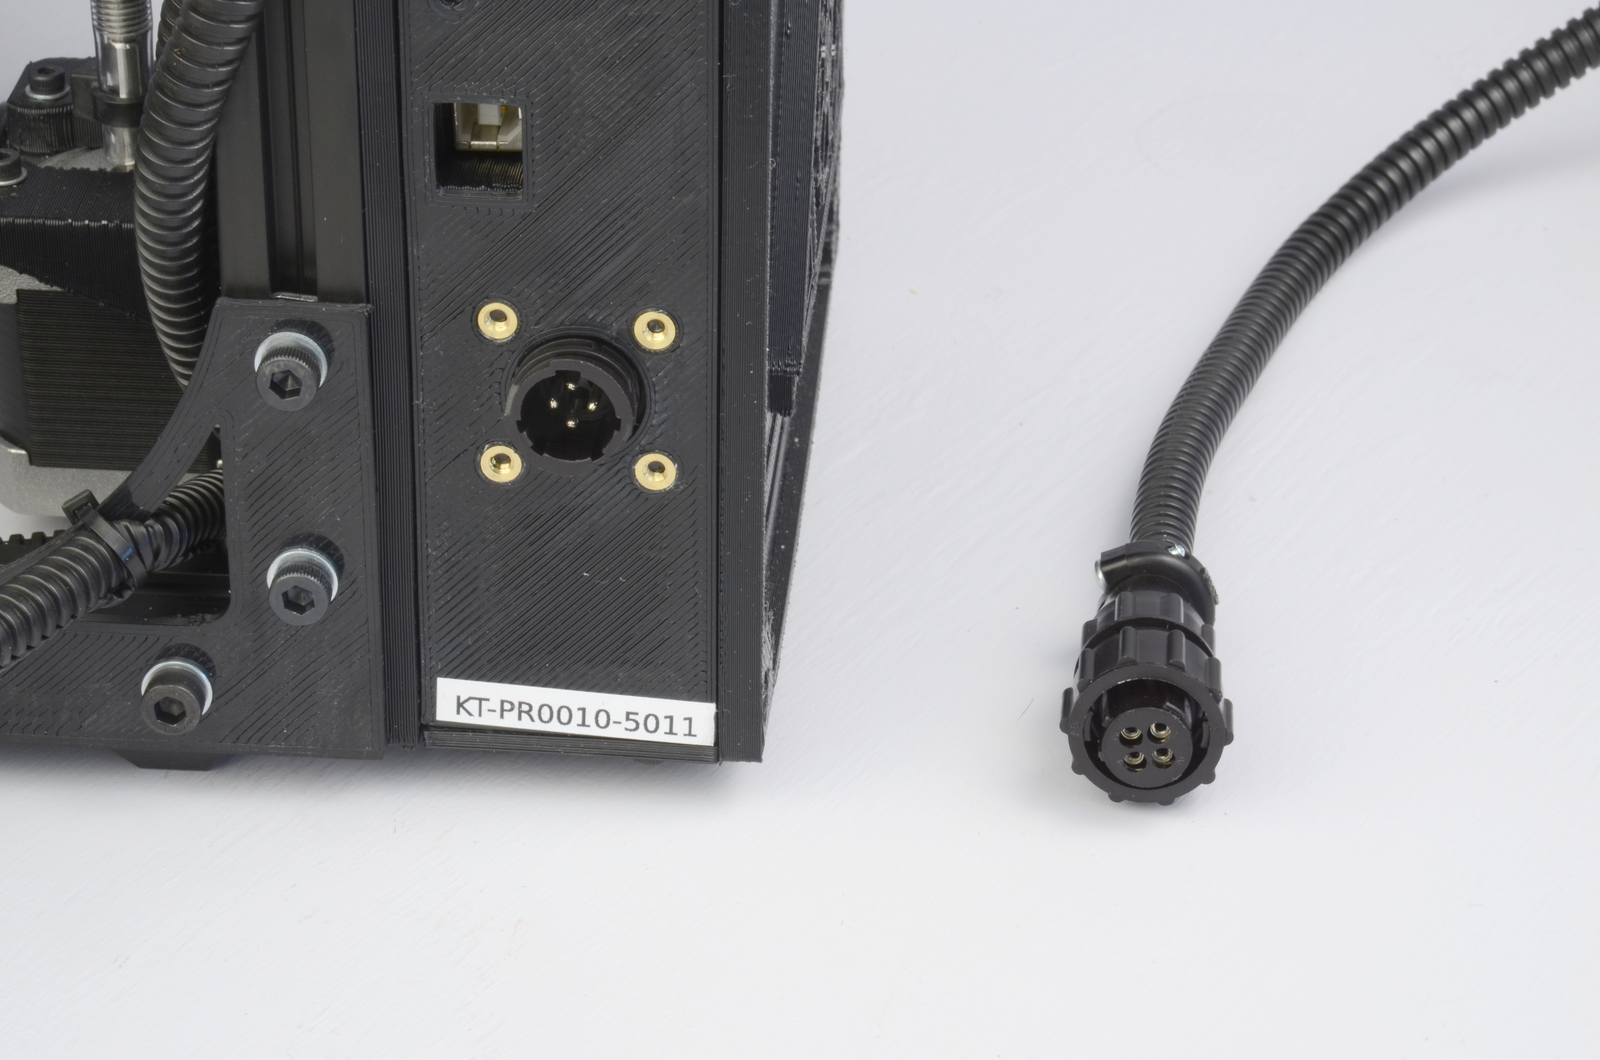
\includegraphics[keepaspectratio=true,angle=0,height=0.4\textheight,width=1.0\textwidth]{electronics_DC_connector.JPG}
\caption{12V DC Power supply plug and receptacle}
\label{fig:ps_plug}
\end{figure}

%\begin{figure}[hp]
\begin{figure}[H]
\centering
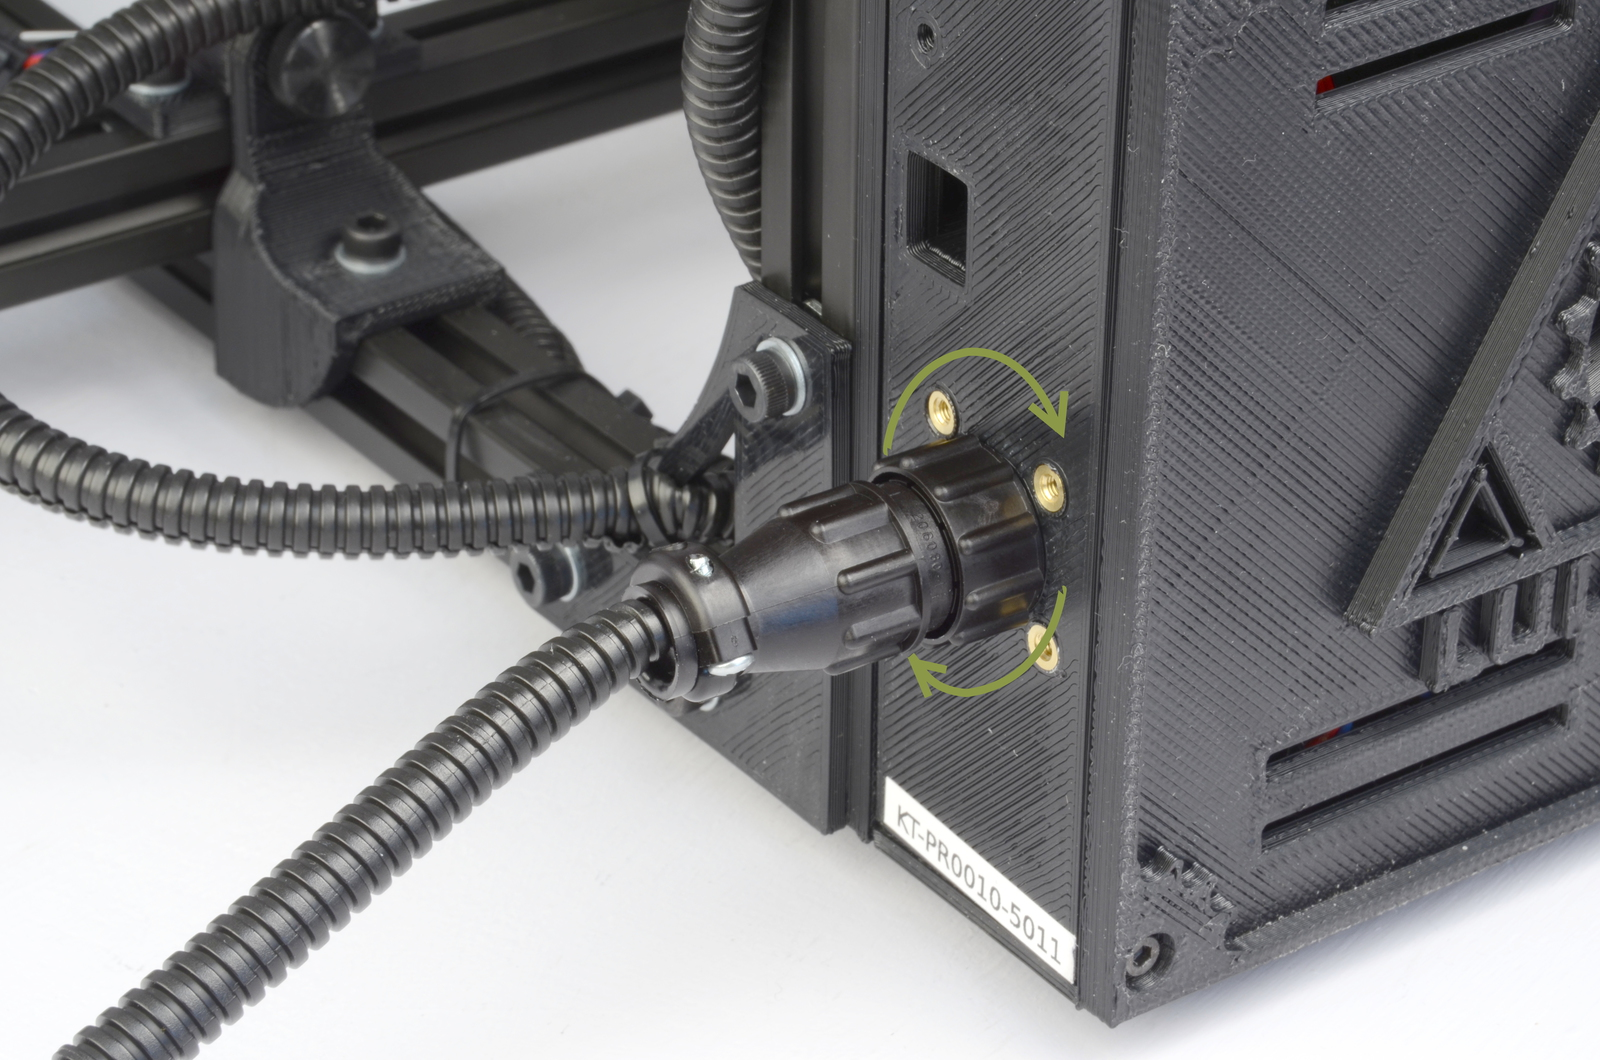
\includegraphics[keepaspectratio=true,angle=0,height=0.4\textheight,width=1.0\textwidth]{electronics_DC_connector_tight.JPG}
\caption{The power supply plug correctly plugged in}
\label{fig:electronics_plugs_plugged-in}
\end{figure}

\item Locate, on the right of the power supply, the red AC voltage switch. Depending on your location you will need to change the AC voltage switch to 115V or 230V. North America is generally 115V and the majority of other regions are 230V. You can find general voltage by country at \texttt{wikipedia.org/wiki/Mains\_electricity\_by\_country}.

\index{RAMBo}
\item Plug in the USB cable, B plug (square plug) side, into the USB receptacle on the printer electronics. Plug the other end of the USB cable, A plug side, into your computer.

\index{PTFE tube}
\item Locate the filament guide with attached PTFE tube
(Fig. \ref{fig:filament_guide}, page \pageref{fig:filament_guide}). The filament guide attaches to the filament guide mount which can be found on the top right side of the printer frame (Fig. \ref{fig:filament_guide_mount}, page \pageref{fig:filament_guide_mount}). The filament guide easily pops on to the guide mount as shown in figure \ref{fig:filament_guide_setting} (pg. \pageref{fig:filament_guide_setting}).
%\begin{figure}[hbt]
\begin{figure}[H]
\centering
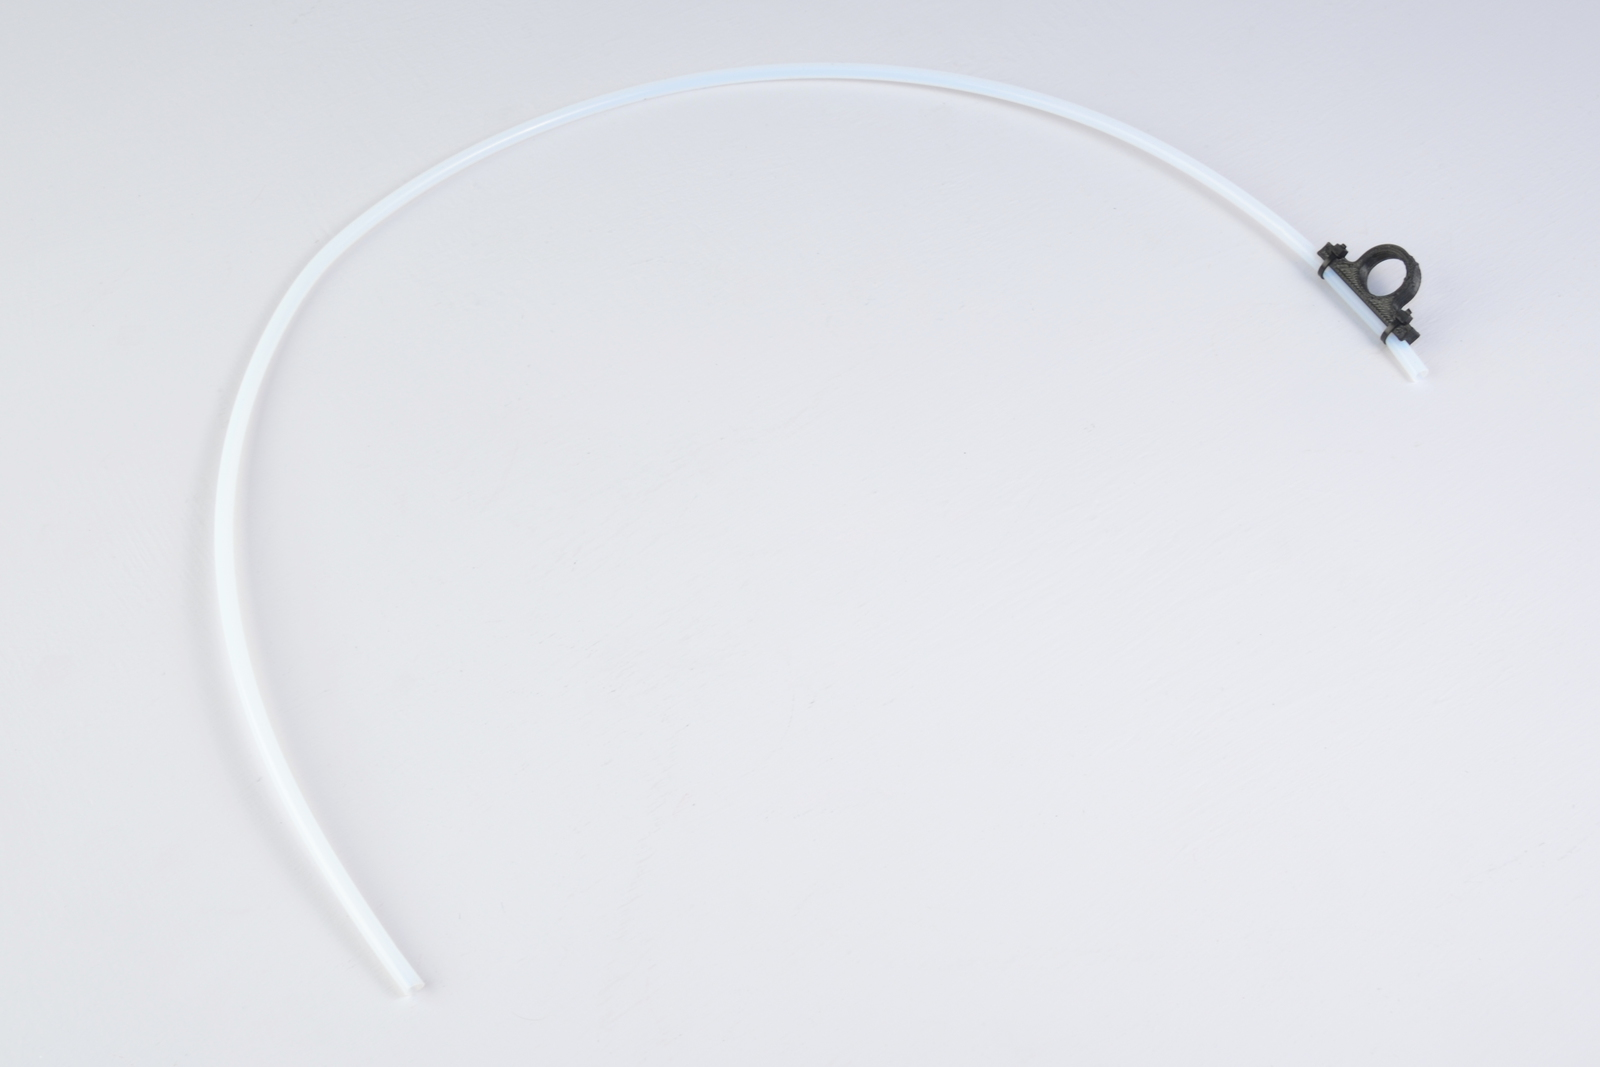
\includegraphics[keepaspectratio=true,angle=0,height=0.4\textheight,width=1.0\textwidth]{filament_guide.JPG}
\caption{Filament Guide}
\label{fig:filament_guide}
\end{figure}

%\begin{figure}[hbt]
\begin{figure}[H]
\centering
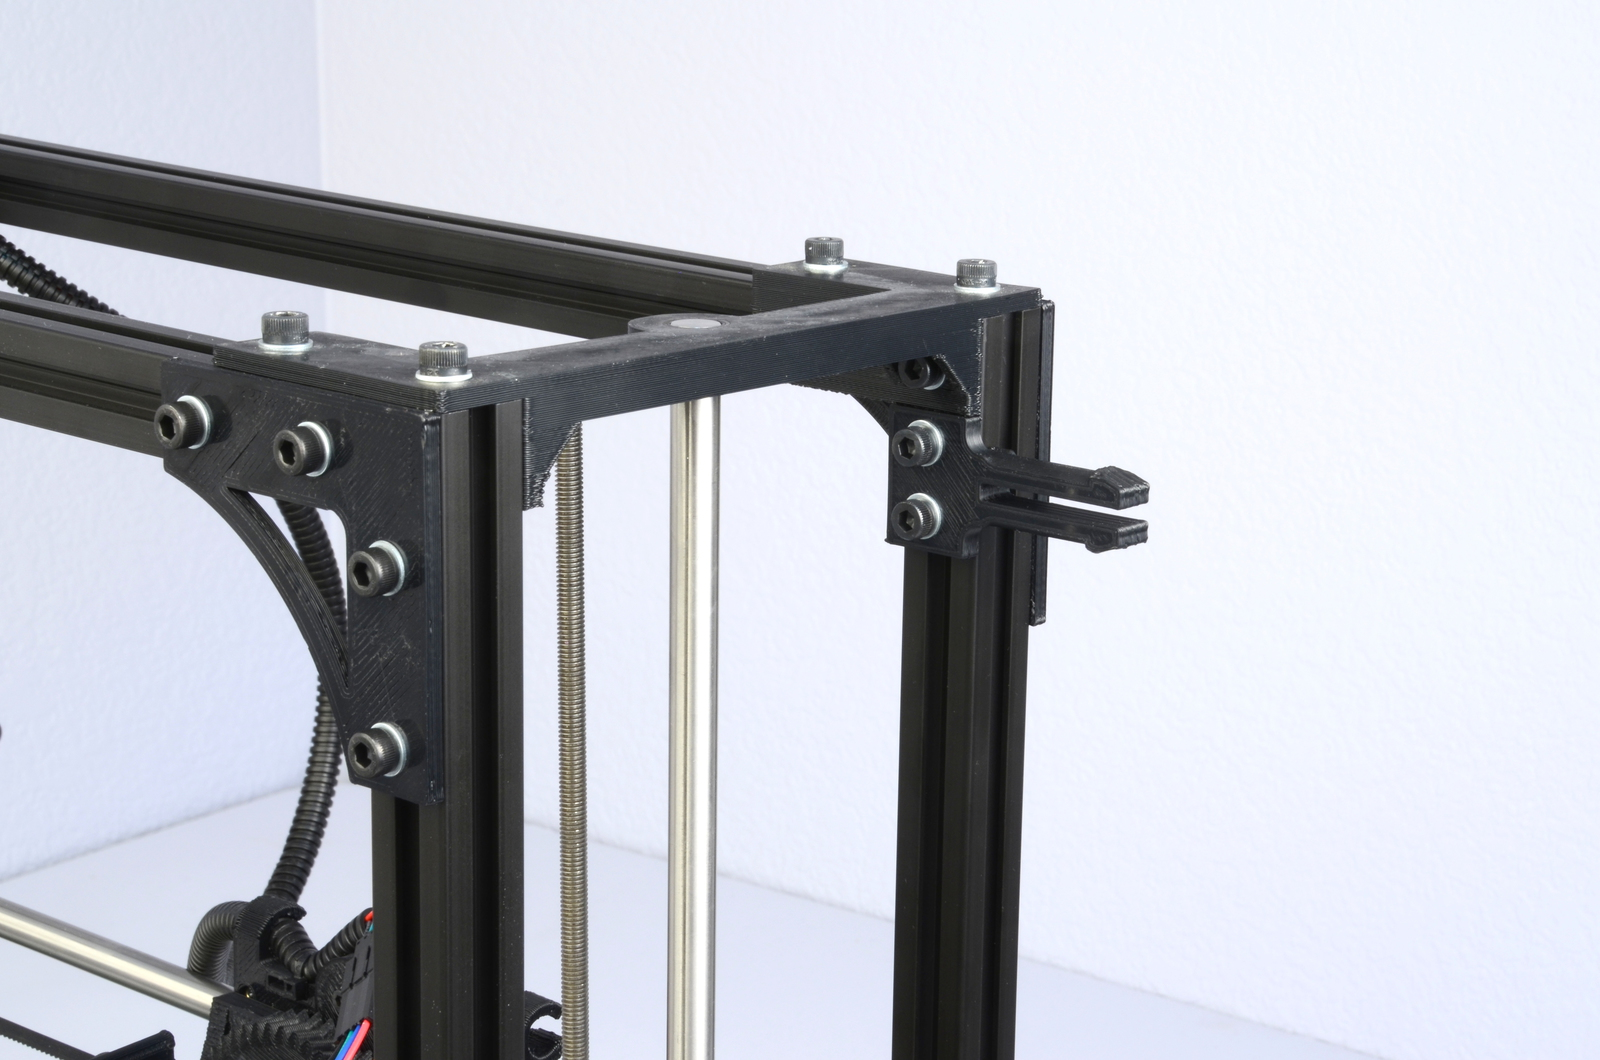
\includegraphics[keepaspectratio=true,angle=0,height=0.4\textheight,width=1.0\textwidth]{filament_guide_mount.JPG}
\caption{Filament Guide Mount}
\label{fig:filament_guide_mount}
\end{figure}

%\begin{figure}[hbt]
\begin{figure}[H]
\centering
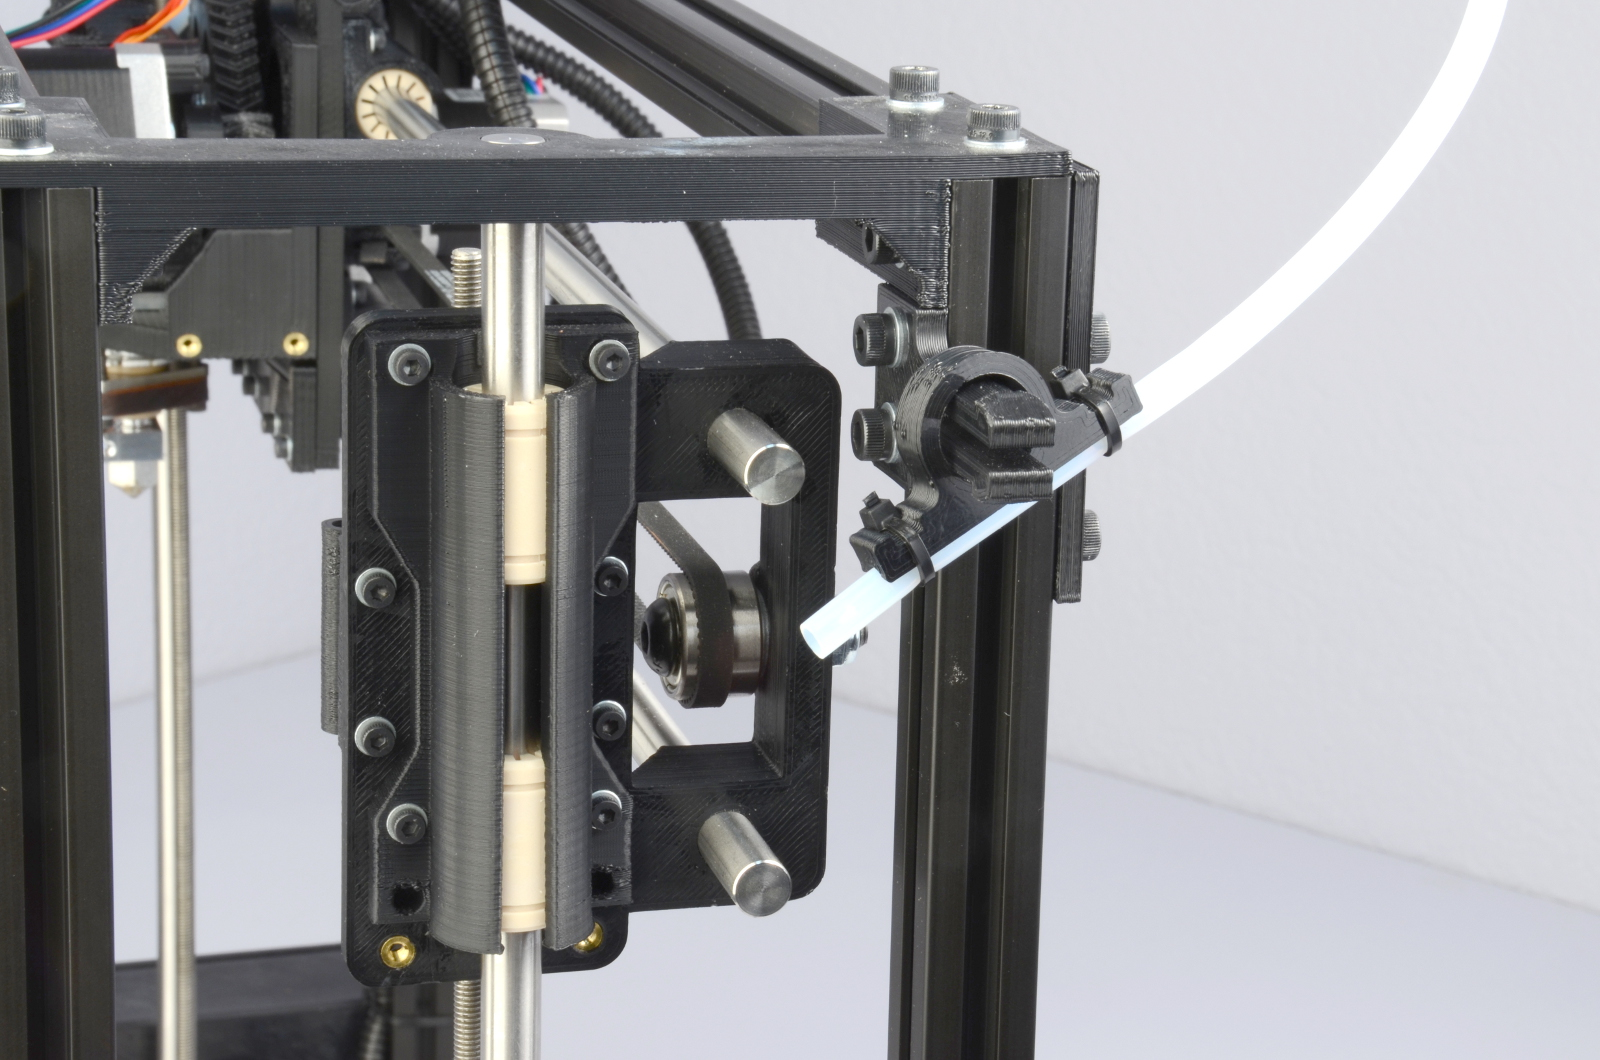
\includegraphics[keepaspectratio=true,angle=0,height=0.4\textheight,width=1.0\textwidth]{filament_guide_direction.JPG}
\caption{Filament Guide Setting}
\label{fig:filament_guide_setting}
\end{figure}

\index{end stops}
\glossary{End stops}{Mechanical or optical switches that are used to mark the 3 home (zero) positions.}
\item Your TAZ 3D printer is now setup and ready to start printing. Before moving forward you should become familiar with the TAZ Cartesian type system. The printer moves in three axes: X, Y, and Z (Fig. \ref{fig:axes}, page \pageref{fig:axes}). These three axes allow the tool head to move to any point within the print area. Note the location of the mechanical end stops which are small switches located at the home point of each axis (Fig. \ref{fig:endstops}, page \pageref{fig:endstops}). Each end stop switch allows the printer to find the 0, the origin, or starting point, of each axis. The mechanical end stops should never be blocked during the initial homing function or during a print.
%\begin{figure}[hbt]
\begin{figure}[H]
\centering
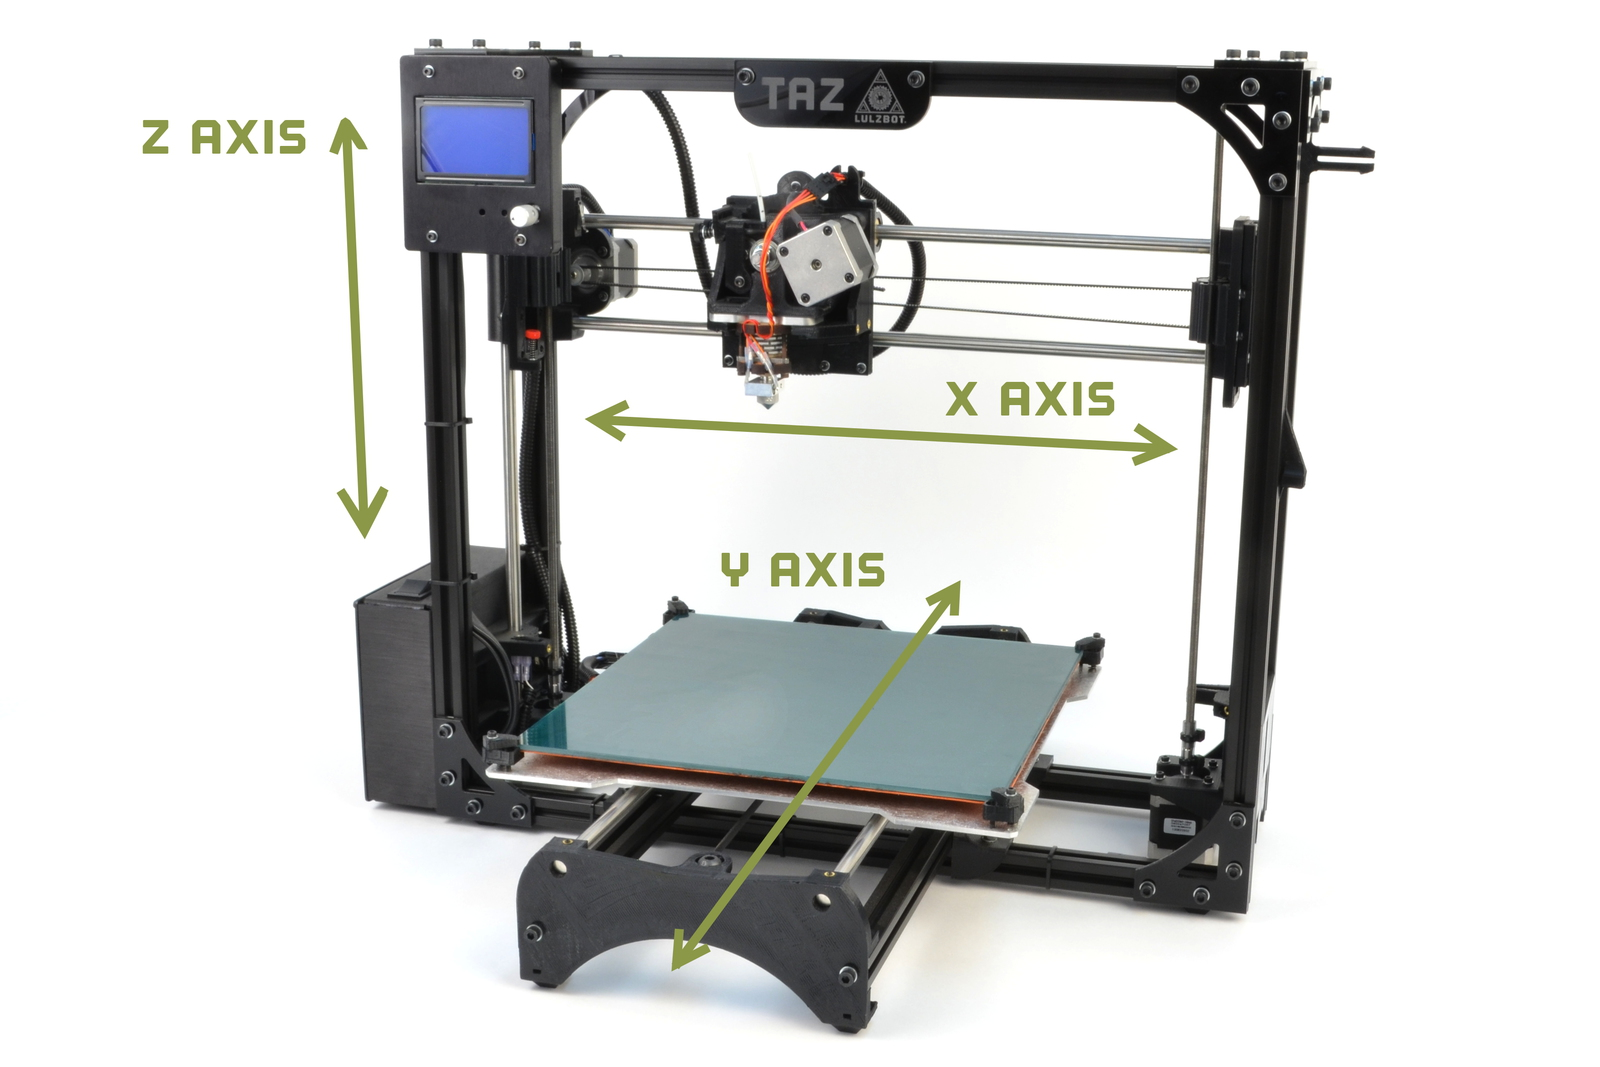
\includegraphics[keepaspectratio=true,angle=0,height=0.4\textheight,width=1.0\textwidth]{axes.JPG}
\caption{Axes movement directions}
\label{fig:axes}
\end{figure}

\begin{figure}[hp]
\centering
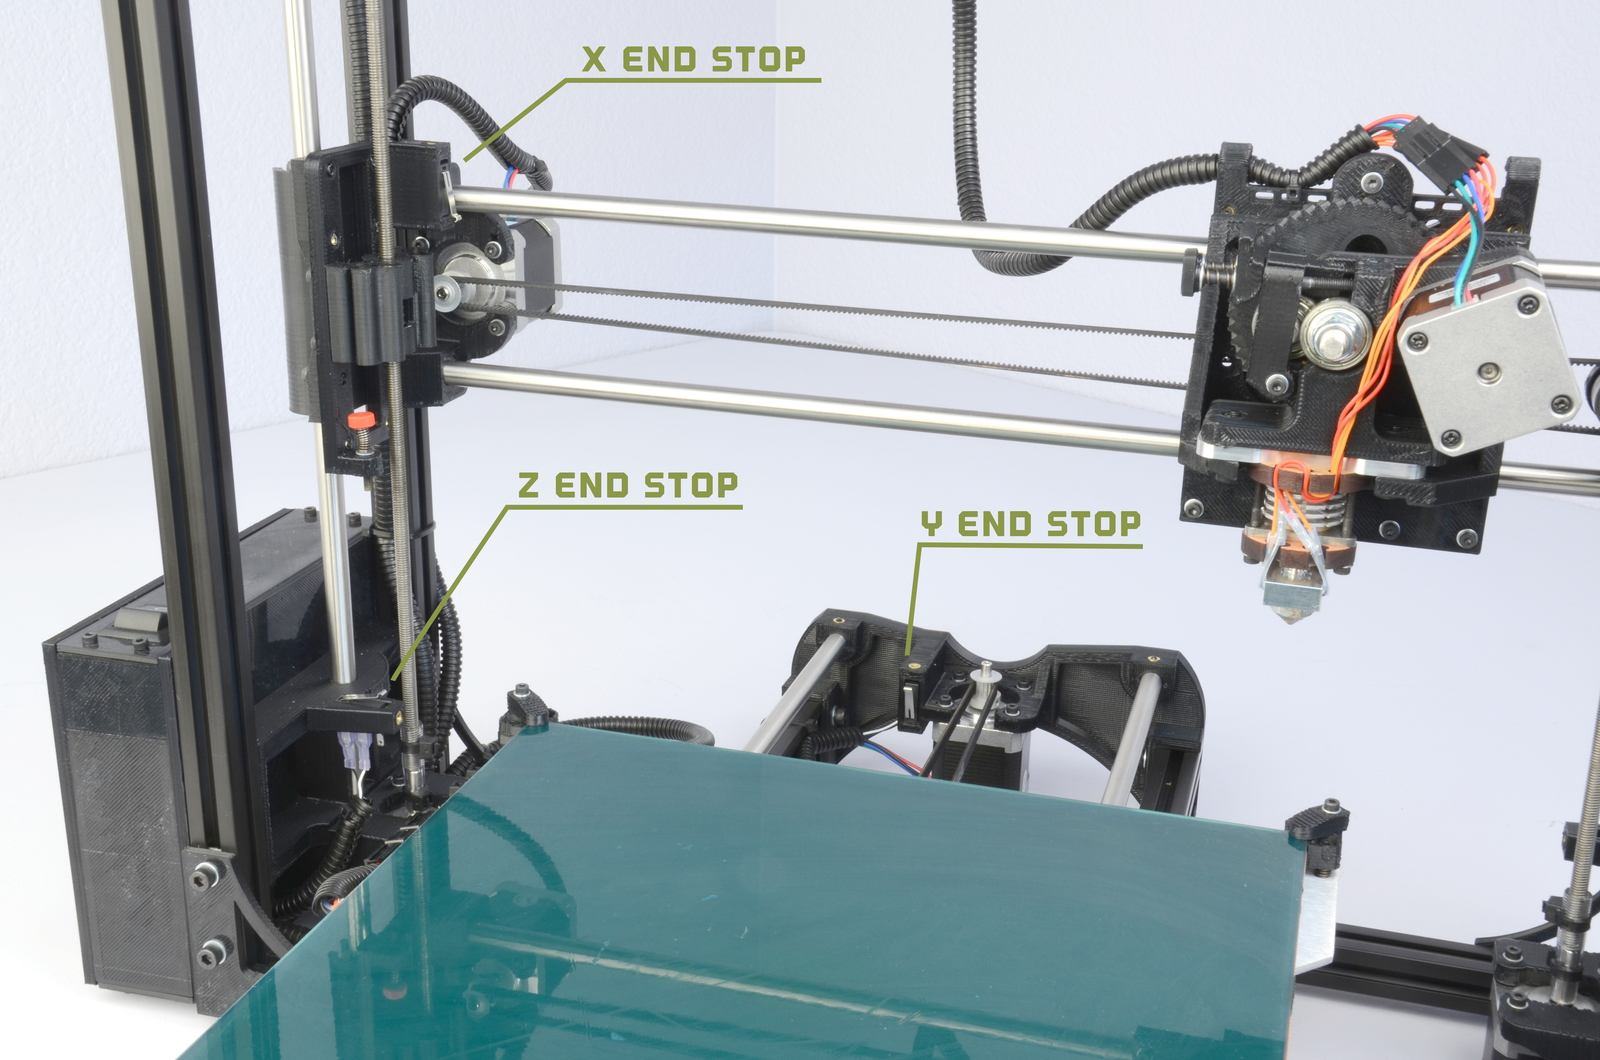
\includegraphics[keepaspectratio=true,angle=0,height=0.4\textheight,width=1.0\textwidth]{end_stop_switches.JPG}
\caption{End stop locations}
\label{fig:endstops}
\end{figure}

\end{enumerate}
}
\fi
%%% END SETUP %%%

%%% FILAMENT %%%
\iffilament
\chapter{\emph{Loading Filament}}
\thispagestyle{empty}
\markboth{Loading Filament}{LulzBot TAZ User Manual}
{%
% Filament.tex
%
% LulzBot TAZ™ User Manual
%
% Copyright (C) 2015 Aleph Objects, Inc.
%
% This document is licensed under the Creative Commons Attribution 4.0
% International Public License (CC BY-SA 4.0) by Aleph Objects, Inc.
%

%%% Copy to Setup.tex, break at the point software is needed. %%%
\index{spool holder}
\index{filament arm}
\index{filament spool}
\index{spool}
\glossary{Spool}{Plastic filament coiled and stored on a plastic reel. Preferred over 1.75-mm filament due to improved feeding and better mounting options.}
\glossary{Filament}{Plastic material in a ``string'' like form, as it is fed to the printer.}
\glossary{ABS}{Acrylonitrile butadiene styrene thermoplastic. Usually extrudes at 230C.}
\glossary{PLA}{Polylactic acid is a corn-based biodegradable polymer. Usually extrudes at 185C.}
\glossary{HDPE}{High-density polyethylene.}
\glossary{Polycarbonate}{A strong and impact-resistant thermoplastic. Usually extrudes at ~300C.}
\glossary{HIPS}{High-impact polystyrene.}
\glossary{Laywoo-D3}{Wooden filament similar to PLA. Forty percent of its content consists of recycled wood. Usually prints at ~180C to 210C. Color can be changed by varying the extrusion temperature.}

Before you start printing you will need to load a reel of filament onto the filament arm. The filament arm is meant to work with 1-kg and 5-lb plastic filament reels but can be modified to work with other reel and spool types.

\begin{enumerate}

\item You will find the filament arm on the front right-hand side of the TAZ 3D printer (Figure \ref{fig:filament_arm}, page \pageref{fig:filament_arm}). Place the filament reel on the filament arm with the filament feeding counter-clockwise.

\begin{figure}[H]
\centering
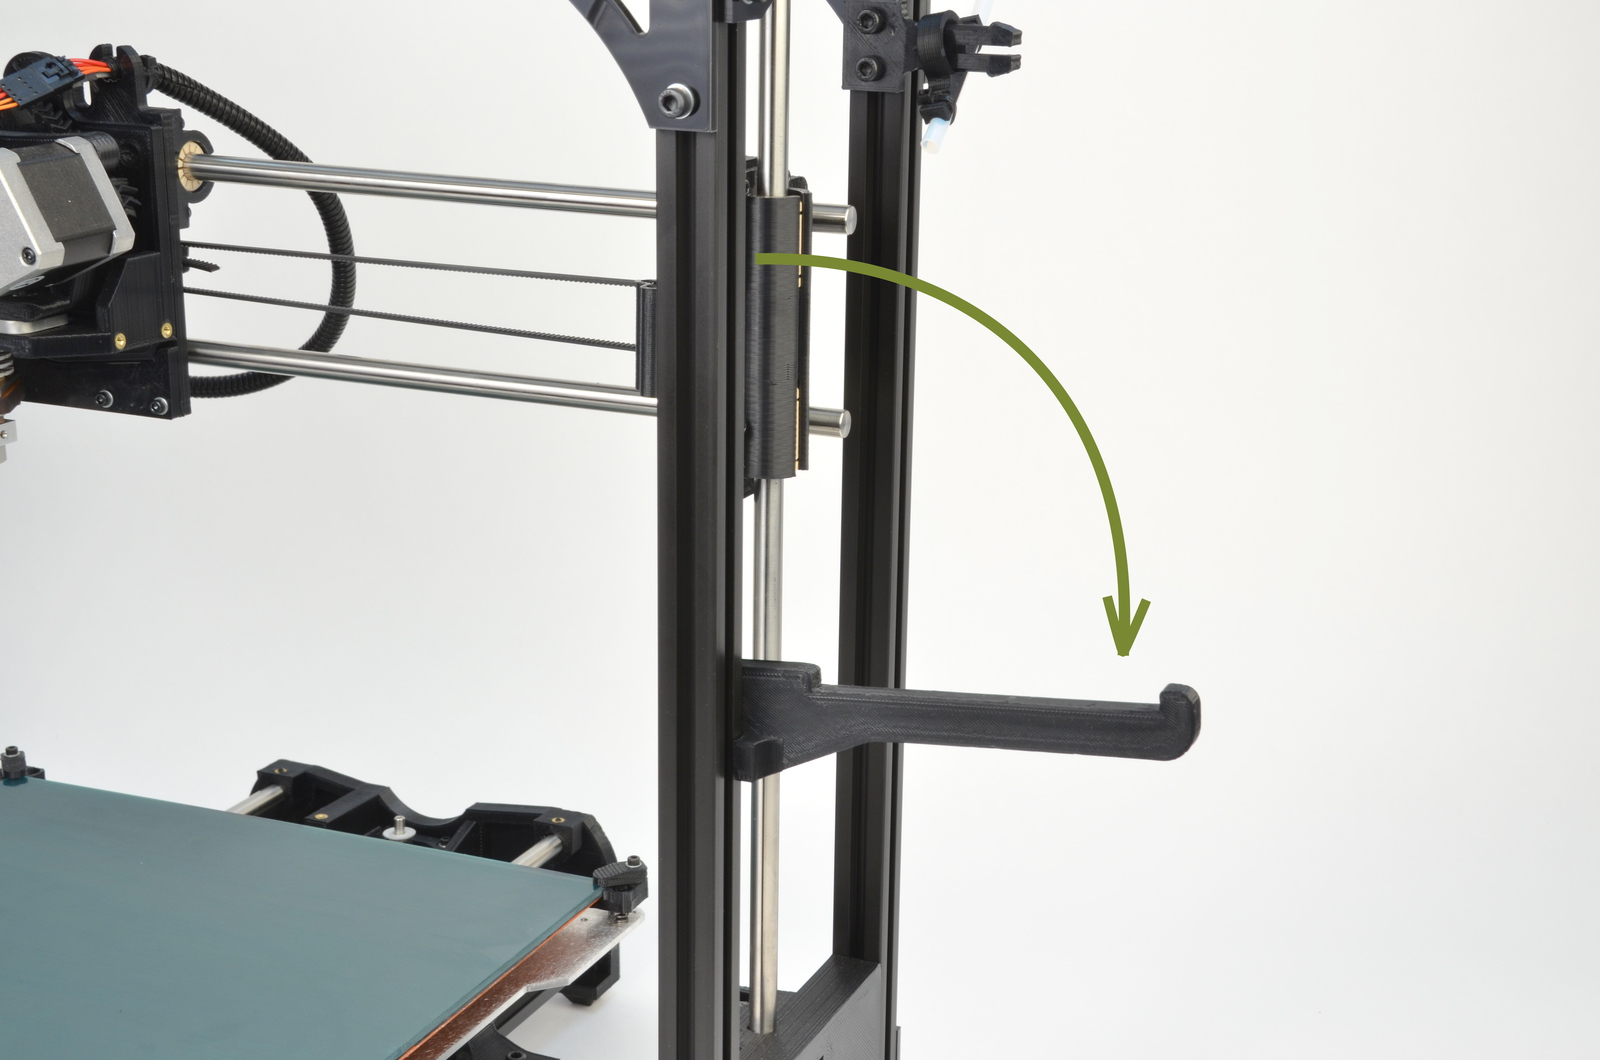
\includegraphics[keepaspectratio=true,angle=0,height=0.4\textheight,width=1.0\textwidth]{filament_arm.JPG}
\caption{Filament reel arm}
\label{fig:filament_arm}
\end{figure}

\index{feed tube}
\item Feed the end of the filament through the filament feed tube. The filament should now be threaded through the PTFE sleeve and exit near the extruder (Figure \ref{fig:filament_arm_loaded}, page \pageref{fig:filament_arm_loaded}).

\begin{figure}[H]
\centering
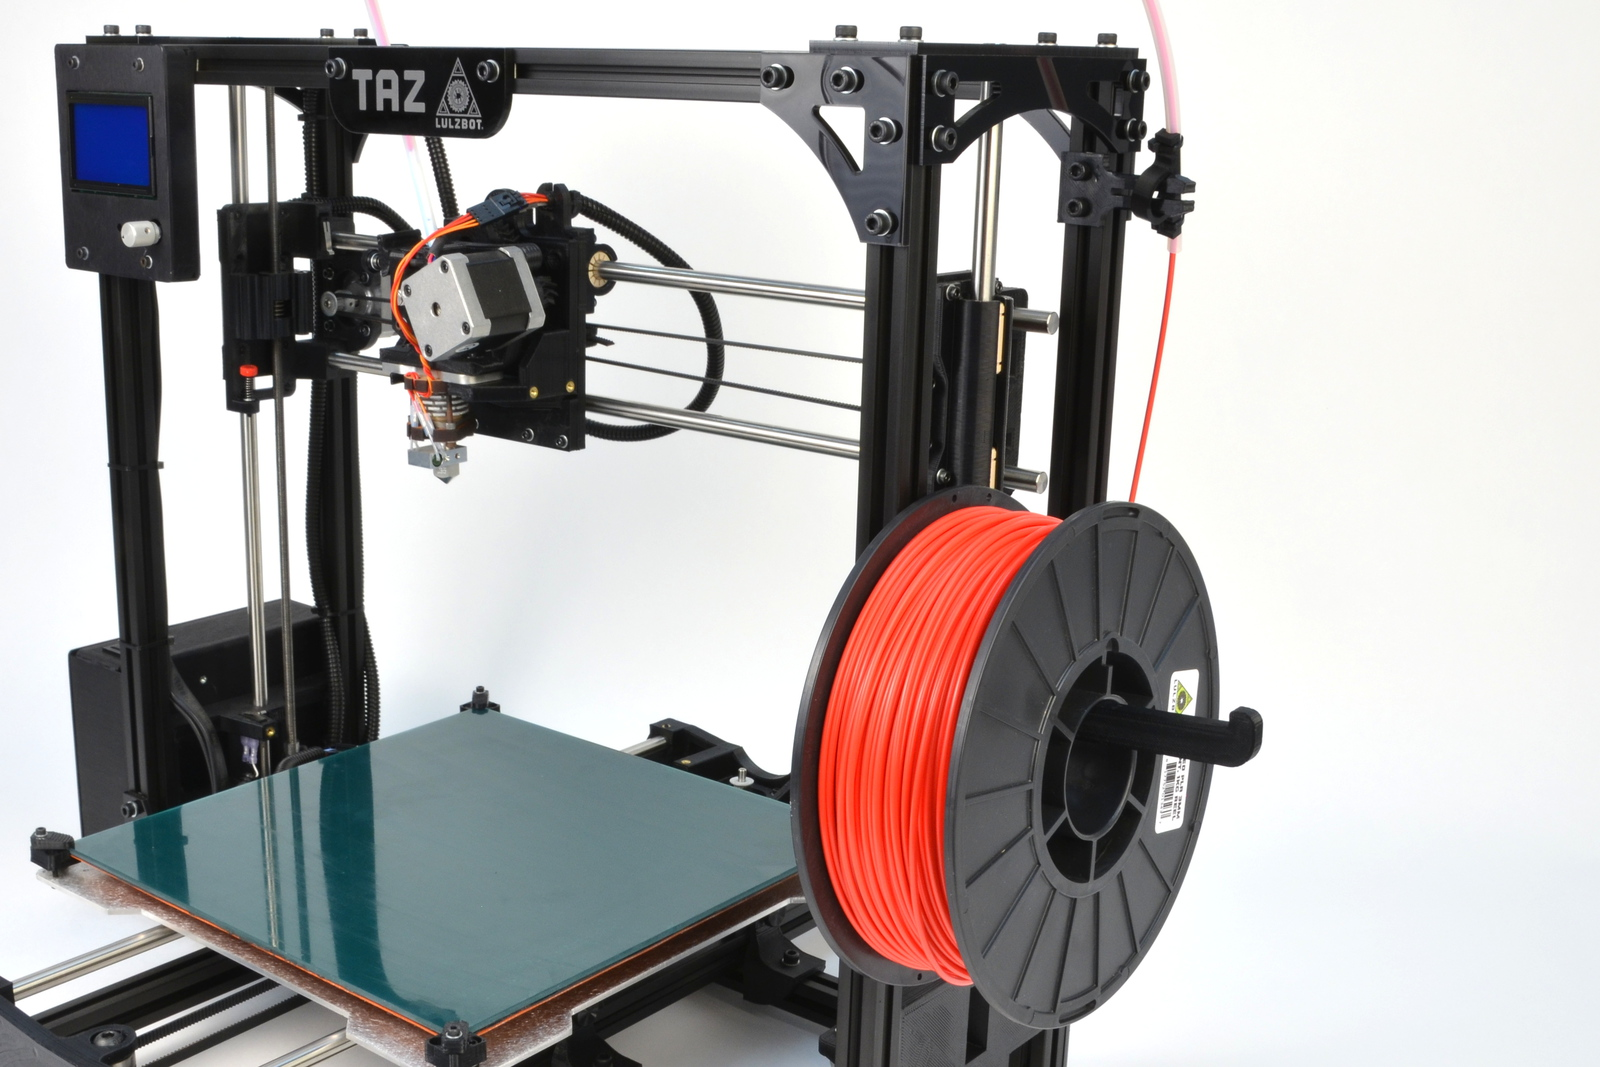
\includegraphics[keepaspectratio=true,angle=0,height=0.4\textheight,width=1.0\textwidth]{filament_arm_loaded.JPG}
\caption{Filament run through the guide}
\label{fig:filament_arm_loaded}
\end{figure}

\item Your filament reel is now mounted and ready for the next steps.

\item When changing filament, slide the opposite end of the filament through one of the holes in the hub of the filament spool. This will keep the filament from unwinding from the spool.

\end{enumerate}
}
\fi
%%% END FILAMENT %%%

%%% SOFTWARE %%%
\ifsoftware
\chapter{\emph{3D Printer Software}}
\thispagestyle{empty}
\markboth{3D Printer Software}{LulzBot TAZ User Manual}
{%
% Software.tex
%
% LulzBot® TAZ User Manual
%
% Copyright (C) 2015 Aleph Objects, Inc.
%
% This document is licensed under the Creative Commons Attribution 4.0
% International Public License (CC BY-SA 4.0) by Aleph Objects, Inc.
%

\section{\texttt{Software Overview}}
\index{software}

To operate your desktop 3D printer you will need to install a few software packages onto your PC. You will need a 3D printer host, an \texttt{.STL} to \texttt{.GCODE} generator, and optional CAD or 3D modeling software.

\texttt{Cura LulzBot\textsuperscript{\miniscule{\textregistered}} Edition is the recommended software for your LulzBot 3D printer.} Download Cura LulzBot Edition by visiting \texttt{LulzBot.com/Cura}.


\glossary{.GCODE}{The file extension for G-Code files}
\glossary{GCODE}{The common name for the most widely used CNC programming language.}
\glossary{CAD}{Computer Aided Design}

\index{GNU/Linux}
\index{OS X}
\index{Windows}
\index{operating system}
All of the following Free/Libre Software packages are available for GNU/Linux, Windows, and OS X. We highly recommend using these programs on GNU/Linux.

\section{\texttt{Software Types}}
\index{Printer Host}
\index{Slicing}
\index{Slicers}
\index{GCODE}
\index{g-code}

\begin{description}
\item{Printer Hosts} \hfill \\
Printer Host software is used to control the 3D printer. The program not only allows you to manually move the printer along all the axes, but set temperatures manually, send commands, and receive feedback/error messages from the onboard electronics. We recommend that new users start with Cura LulzBot\textsuperscript{\miniscule{\textregistered}} Edition as it includes a slicing engine as well.

\item{\texttt{Slicers}} \hfill \\
These programs take the 3-Dimensional model (typically STL/OBJ/etc) and determine the 3D printer toolpath based on the options selected. The slicing engine uses the nozzle diameter, movement speeds, layer height, and other variables to determine the coordinates where it needs to move, and the rates at which it will do so. This information is exported out of the program as a GCODE file. The GCODE file is a plain-text file with a series of text-based codes and a list of the complete X,Y, and Z-axis coordinates used for printing the 3D model. We recommend that new users start with Cura LulzBot Edition as it includes the printer host as well.

%Recommended Slicers:
%\begin{itemize}
%\item Cura LulzBot Edition
%\item Slic3r
%\item Skeinforge
%\item Sfact
%\end{itemize}

\end{description}

\index{download}
\index{driver}
\section{\texttt{Installing Drivers}}
GNU/Linux and OS X users will not need to install a driver to communicate with the LulzBot TAZ 3D printer. Windows users will need to install the drivers. Using Cura LulzBot Edition as your printer host and slicing software is recommended, as the drivers will automatically be installed during the Cura installation process. Download Cura LulzBot Edition by visiting \texttt{LulzBot.com/Cura}. The drivers can also be downloaded from \texttt{LulzBot.com/downloads}. A visual guide showing the driver installation process can be found in our download section as well.


\section{\texttt{CAD and 3D Modeling Software}}
\index{CAD}
\index{software}
\index{STL}

LulzBot is not distributing a CAD or 3D modeling software package. However, multiple Free/Libre Software packages are available. Other common non-free CAD and 3D modeling software are also capable of exporting the required \texttt{.STL} files.

On some CAD and 3D modeling software you will need to select millimeters as the output unit. If possible it is best to build your 3D design in metric units rather than imperial units. Cura requires .STL files sized in millimeters. If an .STL with inches as units is loaded into Cura, the model will be scaled much smaller than expected. You can scale the model by \texttt{25.40} to compensate. The software listed below outputs millimeters as the unit by default.

\subsection{\texttt{FreeCAD}}
\index{FreeCAD}
\index{GNU/Linux}
\index{Windows}
\index{OS X}
Website: \texttt{http://www.freecadweb.org/}

Although still in development, contains a full GUI for building CAD models. FreeCAD is capable of creating simple to complex designs. STL files can also easily be exported for use with 3D printing. FreeCAD is available for GNU/Linux, Windows, and OS X. The latest development version is recommended.

\subsection{\texttt{OpenSCAD}}
\index{OpenSCAD}
\index{GNU/Linux}
\index{Windows}
\index{OS X}
Website: \texttt{http://openscad.org}

OpenSCAD is different than FreeCAD in that it is script based. Rather than using a GUI to generate CAD designs, OpenSCAD CAD designs are created using script based renderings. Users with programming experience would find this useful. Also, OpenSCAD uses a simple script language that is easy for users with little or no programming experience to learn.

\subsection{\texttt{Blender}}
\index{Blender}
\index{GNU/Linux}
\index{Windows}
\index{OS X}
Website: \texttt{http://blender.org}

The most widely used Free/Libre Software 3D modeling software, Blender is well documented with tutorials available on the Blender.org website as well as found online.

\subsection{\texttt{Shapesmith}}
\index{Shapesmith}
Website: \texttt{http://shapesmith.net}

Shapesmith is a web-based 3D modeling software. This means there is no required software to get started designing models. Shapesmith is also a great choice for anyone starting out in CAD/ 3D modeling.

\section{\texttt{Alternative Printer Host Software}}
\index{Host}
\index{software}
\index{STL}

\subsection{\texttt{OctoPrint}}
\index{OctoPrint}
\index{GNU/Linux}
\index{Windows}
\index{OS X}
Website: \texttt{http://octoprint.org/}

Octoprint is a printer host that uses a web-based interface to access and control your 3D printer. Added web-cam functionality allows for time-lapse videos and a live stream. Octoprint will run on GNU/Linux, Windows, OS X based computers and can even run well on a Beagle Bone Black or a RaspberryPi (inexpensive business-card sized computers).

\subsection{\texttt{BotQueue}}
\index{BotQueue}
\index{GNU/Linux}
\index{OS X}
Website: \texttt{https://www.botqueue.com/}

BotQueue works well for those users wanting to have a web-based multiple 3D printer operation running off a queuing system.


\subsection{\texttt{MatterControl}}
\index{MatterControl}
%\index{GNU/Linux}
\index{Windows}
\index{OS X}
Website: \texttt{http://www.mattercontrol.com/}

MatterControl is another printer host that currently runs on GNU/Linux, Windows, and OS X. It features 2D and 3D model viewing, a print queue, and print file organization and searching.

\subsection{\texttt{Source Files}}
\index{Source Files}
Aleph Objects, Inc., the maker of the LulzBot\textsuperscript{\miniscule{\textregistered}} TAZ 3D printer, completely supports Free Software, Libre Innovation, and Open Source Hardware. Along with the LulzBot TAZ 3D printer being a Free Software and Open Source Hardware design, it has been tested to work with 100\% Free/Libre Software. Our source code and design files are hosted on:

\begin{description}
\item [LulzBot Download Server] \texttt{http://download.lulzbot.com}
\item [LulzBot Development Server] \texttt{http://devel.lulzbot.com}
\item [Aleph Objects Code Repository] \texttt{http://code.alephobjects.com}
\item [Aleph Objects Download Server] \texttt{http://download.alephobjects.com}
\item [Aleph Objects Development Server] \texttt{http://devel.alephobjects.com}
\end{description}

\glossary{Free Software}{Free Software (or Free/Libre Software) can be thought of as ``free as in free speech, not just free as in free beer'', although most Free Software is available for no cost. Free Software can be copied, modified and is freely available for download.}
\glossary{Libre Innovation}{Aleph Objects uses Free/Libre Software to build and improve Open Source Hardware so that everything we create is free to be viewed, copied, and/or modified by anyone.}
\glossary{Open Source Hardware}{Open source hardware is hardware whose design is made publicly available so that anyone can study, modify, distribute, make, and sell the design or hardware based on that design. The hardware source, the design from which it is made, is available in the preferred format for making modifications to it. For more information visit \texttt{http://www.oshwa.org/definition/}.}


}
\fi
%%% END SOFTWARE %%%


%%% CURA %%%
\ifcura
\chapter{\emph{Cura LulzBot Edition}}
\thispagestyle{empty}
\markboth{Cura LulzBot Edition}{LulzBot TAZ User Manual}
{%
% Cura.tex
%
% LulzBot Cura User Manual
%
% Copyright (C) 2015 Aleph Objects, Inc.
%
% This document is licensed under the Creative Commons Attribution 4.0
% International Public License (CC BY-SA 4.0) by Aleph Objects, Inc.
%

\section{Cura}
\index{Cura}
\label{Cura}
\glossary{Cura}{Cura is a cross-platform software package that combines a slicing engine with a printer host interface.}
\glossary{Slic3r}{Slic3r is a cross-platform 3D model slicing engine. It's used to process the 3 dimensional model into the Gcode (tool path) needed to physically generate the print.}

\subsection{Setup Cura}
\index{Installation}
Cura is available for download on our website at \texttt{http://LulzBot.com/cura}. When installing, it is recommended to uninstall any previous versions of Cura you may have been using. 
When first opening Cura, you will be prompted to go through the \texttt{First run wizard}. This will consist of selecting your printer, hot end type, extruder type, and then your nozzle size.

\textcolor{red}{It is important to select the correct printer, hot end, tool head, and nozzle size as Cura uses custom profiles and machine settings based upon which printer, hot end, tool head, and nozzle you are running.}

\begin{itemize}
\item Download the appropriate installer for your computer operating system. Instructions on installation for each operating system is available at \texttt{http://LulzBot.com/cura}.
\item Install Cura by double clicking on the installer.
%\item Once your language has been selected, select \texttt{Next}.
%\item Select \texttt{LulzBot Mini}.
\item Select \texttt{LulzBot TAZ 4 or 5}, then select \texttt{Next}.
\item Select \texttt{Stock TAZ 5 (PEI and Hex V2)}. Press \texttt{Next}.
\item Choose the correct nozzle size for your machine. Your TAZ 5 comes with a \texttt{0.5mm nozzle} standard.
%\item The final step will be a firmware update. \textcolor{red}{Skip this step if you are not switching to different tool heads.} If you are adding on a different tool head, please be sure to update the firmware.
\item Select finish.
\end{itemize}



Once the installation wizard finishes you can move forward with your first print! Start Cura by launching it from your list of installed applications.


\section{Quick Print Settings}
\index{Quick Print Settings}
\begin{figure}[H]
\centering
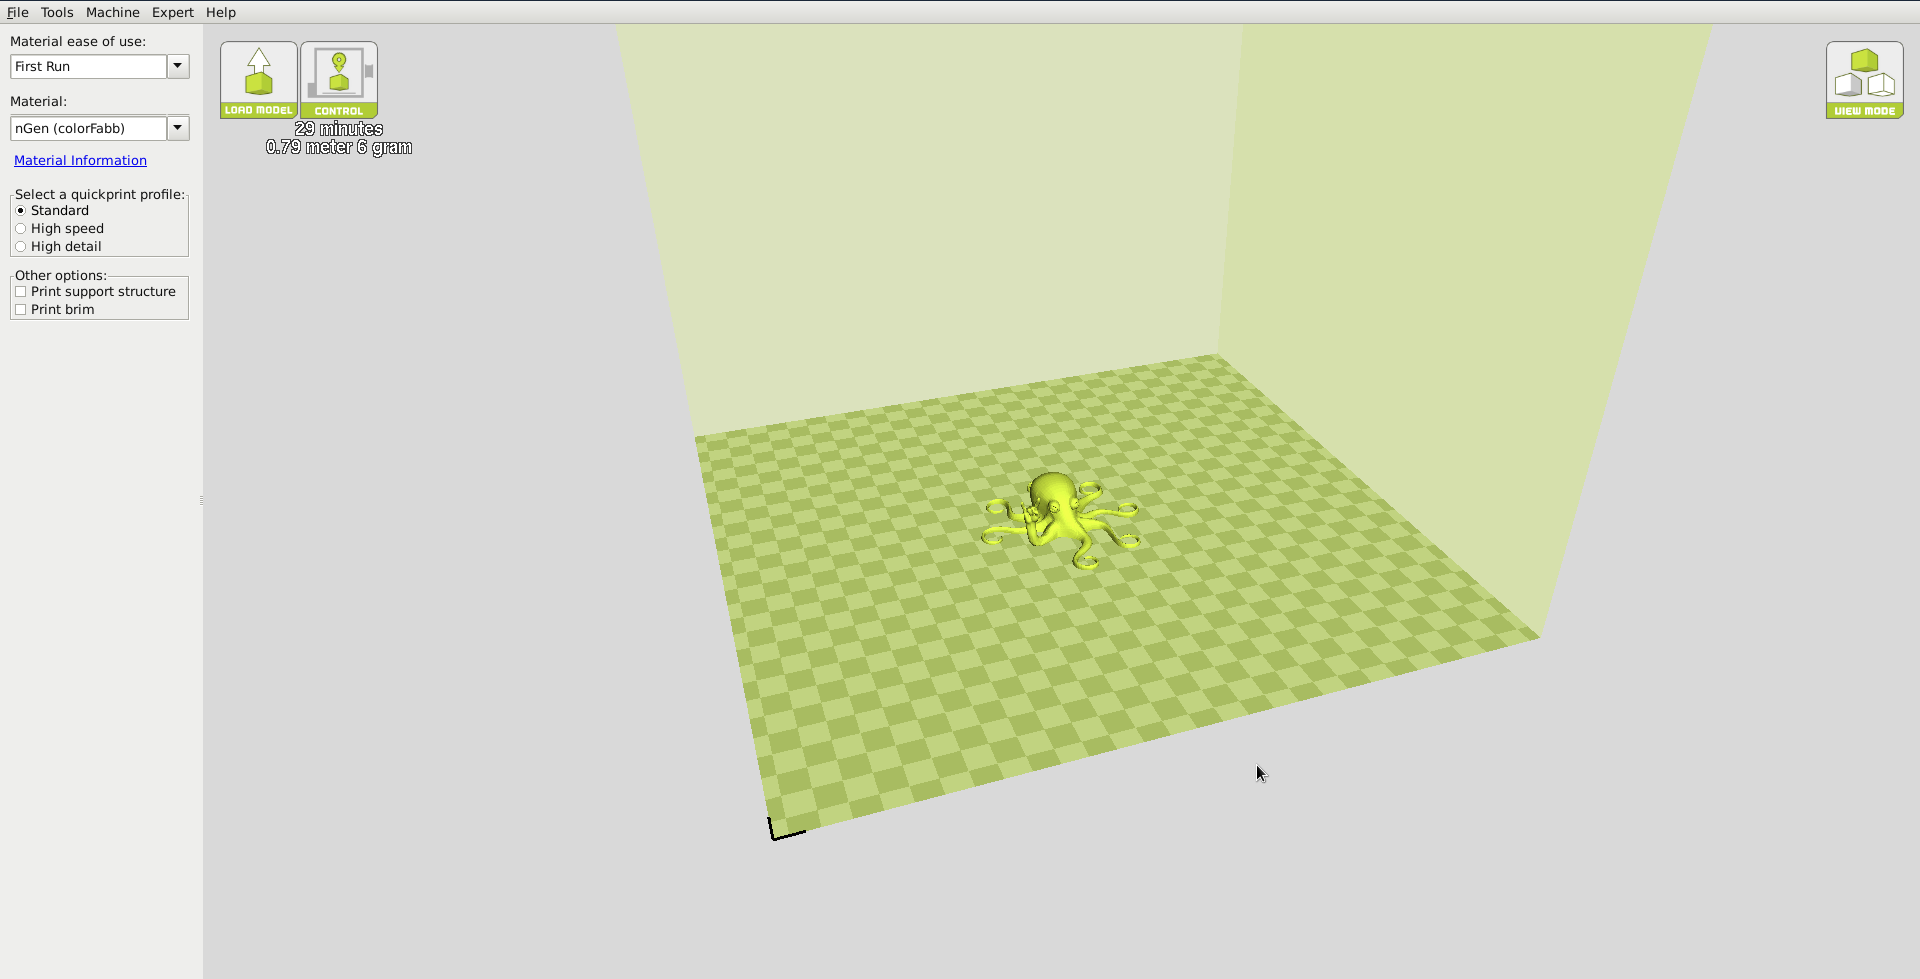
\includegraphics[keepaspectratio=true,angle=0,height=0.4\textheight,width=1.0\textwidth]{quickprintfirstrun.png}
\caption{Quick Print Settings}
\label{fig:Cura}
\end{figure} 
% (photo highlighting profile, material, diameter, and other)
After setting up Cura for the first time, you will be shown the main interface screen. (Fig. \ref{fig:Cura}, page \pageref{fig:Cura}): 

\subsection{Selecting a Quick Print Profile}
\index{Quick Print Profile}
\index{Resolution}
\glossary{Resolution}{In general terms, the resolution you print at can be determined by the layer height you use. The LulzBot\textsuperscript{\miniscule{\texttrademark}} TAZ can print at a layer height of 0.05mm to 0.50mm.}
The print quality settings can be found in the top left-hand corner of the window. For most filaments, there will be Standard, High Speed, and High Detail options. Some of the more exotic filaments may only have a Normal/Standard profile.

\begin{description}
\item[High Detail] \hfill \\
Designed to give greater detail and finer objects. This will have a smaller layer height, which will make each layer thinner, so that curves seem more natural and walls seem less noticeable. This setting will also require more layers to be laid down, increasing overall print time.
\index{High Detail}

\item[Standard] \hfill \\
Designed to give a medium resolution, by increasing the layer height and print speeds. This will make the organic curves slightly more step-like than the fine setting, but will reduce printing time.
\index{Standard Quality}

\item[High Speed] \hfill \\
Designed for the fast prints, where overall model finish is not of concern. Most commonly used for quick iteration of designs found in rapid prototyping.
\index{High Speed}
\end{description}

\subsection{Material Selection}
\index{Material Selection}
\index{filament}
Choose your desired filament. The TAZ ships with a 1 meter sample of ABS, that should be used in your first print.
%If you are not using LulzBot supplied filament, update your filament diameter to your specific average filament diameter. Do this by taking 10 to 12 filament diameter measurements from different parts of the reel and averaging them. Update your filament diameter. You may also want to adjust the temperature, as different manufacturers have different recommended temperatures. % This could be better served in the Full Settings explanation.

\subsection{Printing Support Material}
\index{Support Material}
%%%% Saved for standalone Cura Manual %%%%
%The TAZ and Mini are able to print models that have angles and overhangs, even without support material depending on the overhang distance and angle. Turn this option on if your model could benefit from support material.
%MINI% The Mini 3D printer is able to print models that have angles and overhangs, even without support material depending on the overhang distance and angle. Turn this option on if your model could benefit from support material.
The TAZ 3D printer is able to print models that have angles and overhangs, even without support material depending on the overhang distance and angle. Turn this option on if your model could benefit from support material.

\subsection{Brim}
\index{Brim}
Brim is used to increase surface area of the part you're printing, thereby ensuring proper part adhesion. This will print a single layer high edge around the outside of the part, helping first layer adhesion and minimizing warping.

\subsection{Load Model File}
\index{Load Model}
\index{STL}
Select the STL model you would like to print. Either use the \texttt{Load Model} button or select \texttt{File} > \texttt{Load Model}. Once the file has been loaded, you will see a 3D rendering of your object on the build platform. Select the model to see the various options. 

\subsection{Model Orientation}
\index{Orientation}
Move your model to change where it is printed on the build plate. Do this by left clicking on the model and dragging it to the desired location. The \texttt{black} outlined corner of the 3D print bed view represents the front left hand corner of the build plate on your printer. By holding down the right mouse button and dragging, you can view your model from different angles. %Not sure if this last sentence should be reworked or put in a separate section.
\begin{figure}[H]
\centering
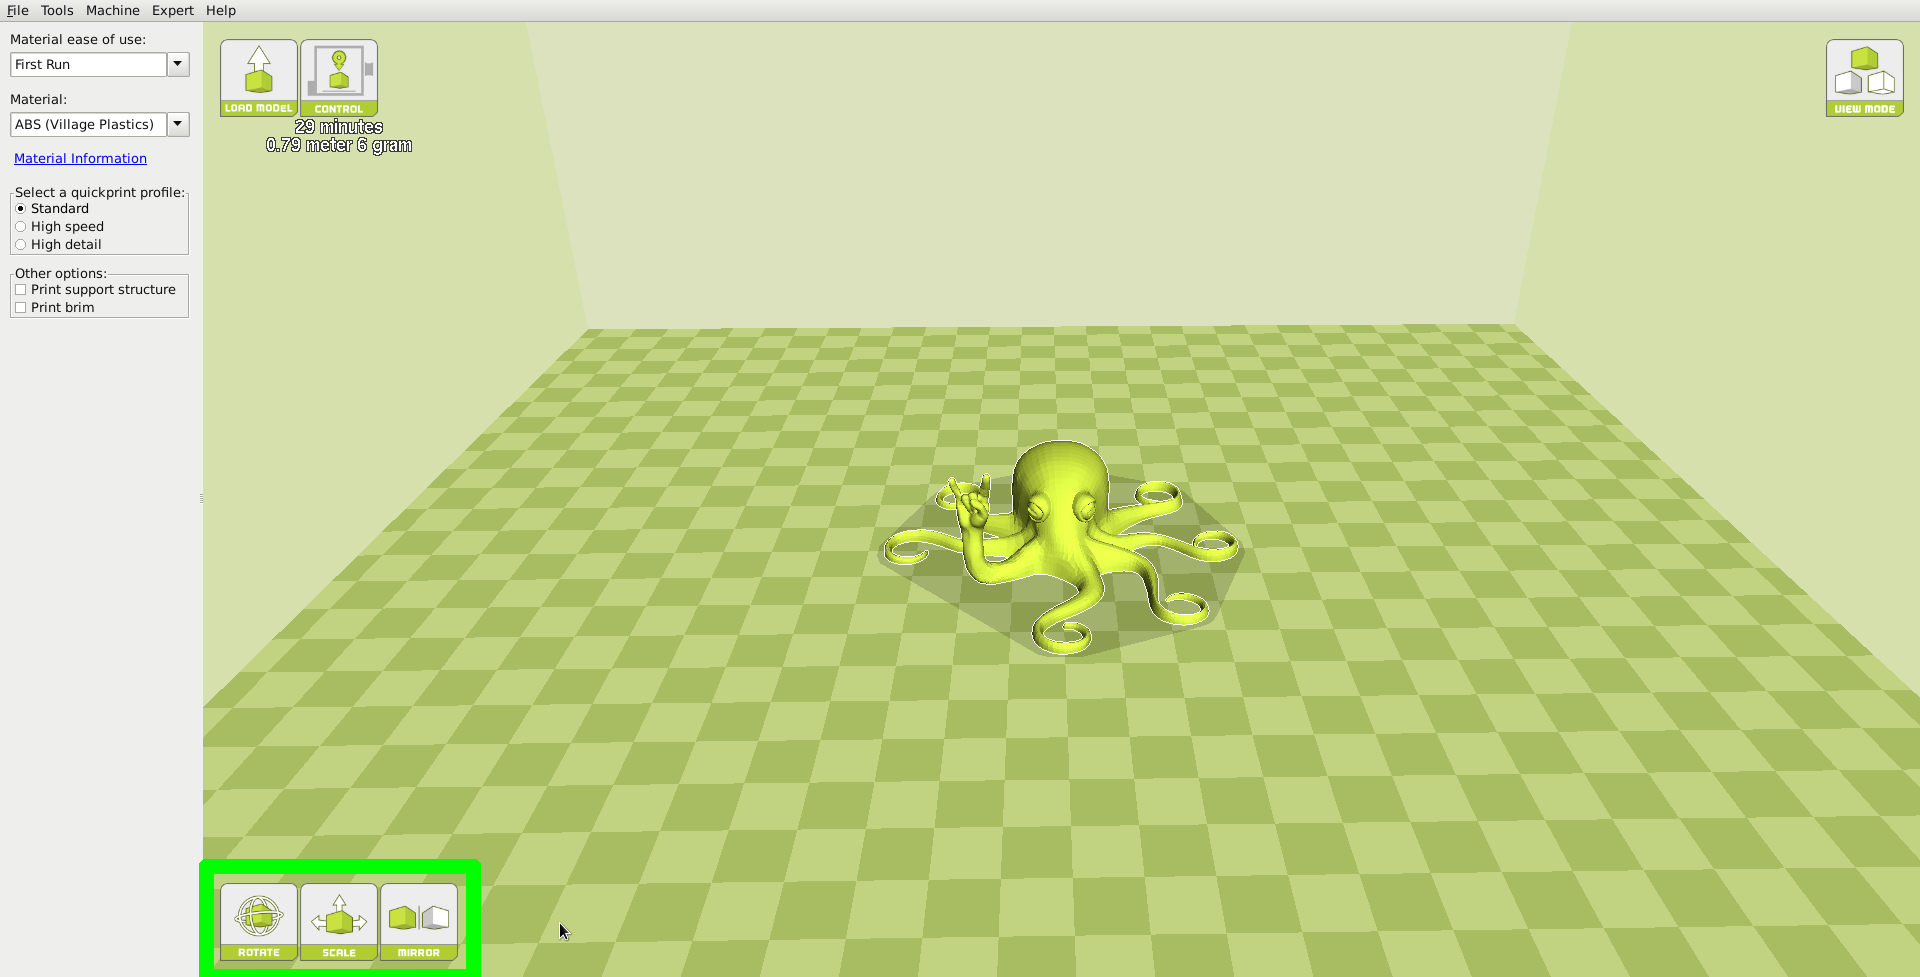
\includegraphics[keepaspectratio=true,angle=0,height=0.4\textheight,width=1.0\textwidth]{optionsTAZ.png}
\caption{Options after selecting model}
\label{fig:Orientation}
\end{figure}

\subsubsection{Rotate}
%%%% Alternate explanation %%%%
%The \texttt{Rotate} button will give you the ability orient your model in along all three axes. Once you click the rotate button, three circles will surround your model. The red circle will allow you to rotate in the XY plane. The Yellow circle will rotate in the XZ plane. The Green circle will rotate in the YZ plane.
\definecolor{yellow1}{cmyk}{0,0,1,0.30}
\definecolor{green1}{rgb}{0.30,1,0.30}
The \texttt{Rotate} button will give you the ability to orient your model in along all three axes. Once you click the rotate button, three circles will surround your model. The \textcolor{red}{red circle} will allow you to rotate around the \textcolor{red}{Z axis}. The \textcolor{yellow1}{Yellow circle} will rotate around the \textcolor{yellow1}{Y axis}. The \textcolor{green1}{Green circle} will rotate around the \textcolor{green}{X axis}. Cura defaults to 15 degree increments. Hold \texttt{Shift} to rotate by \texttt{One Degree Increments}.
\begin{figure}[H]
\centering
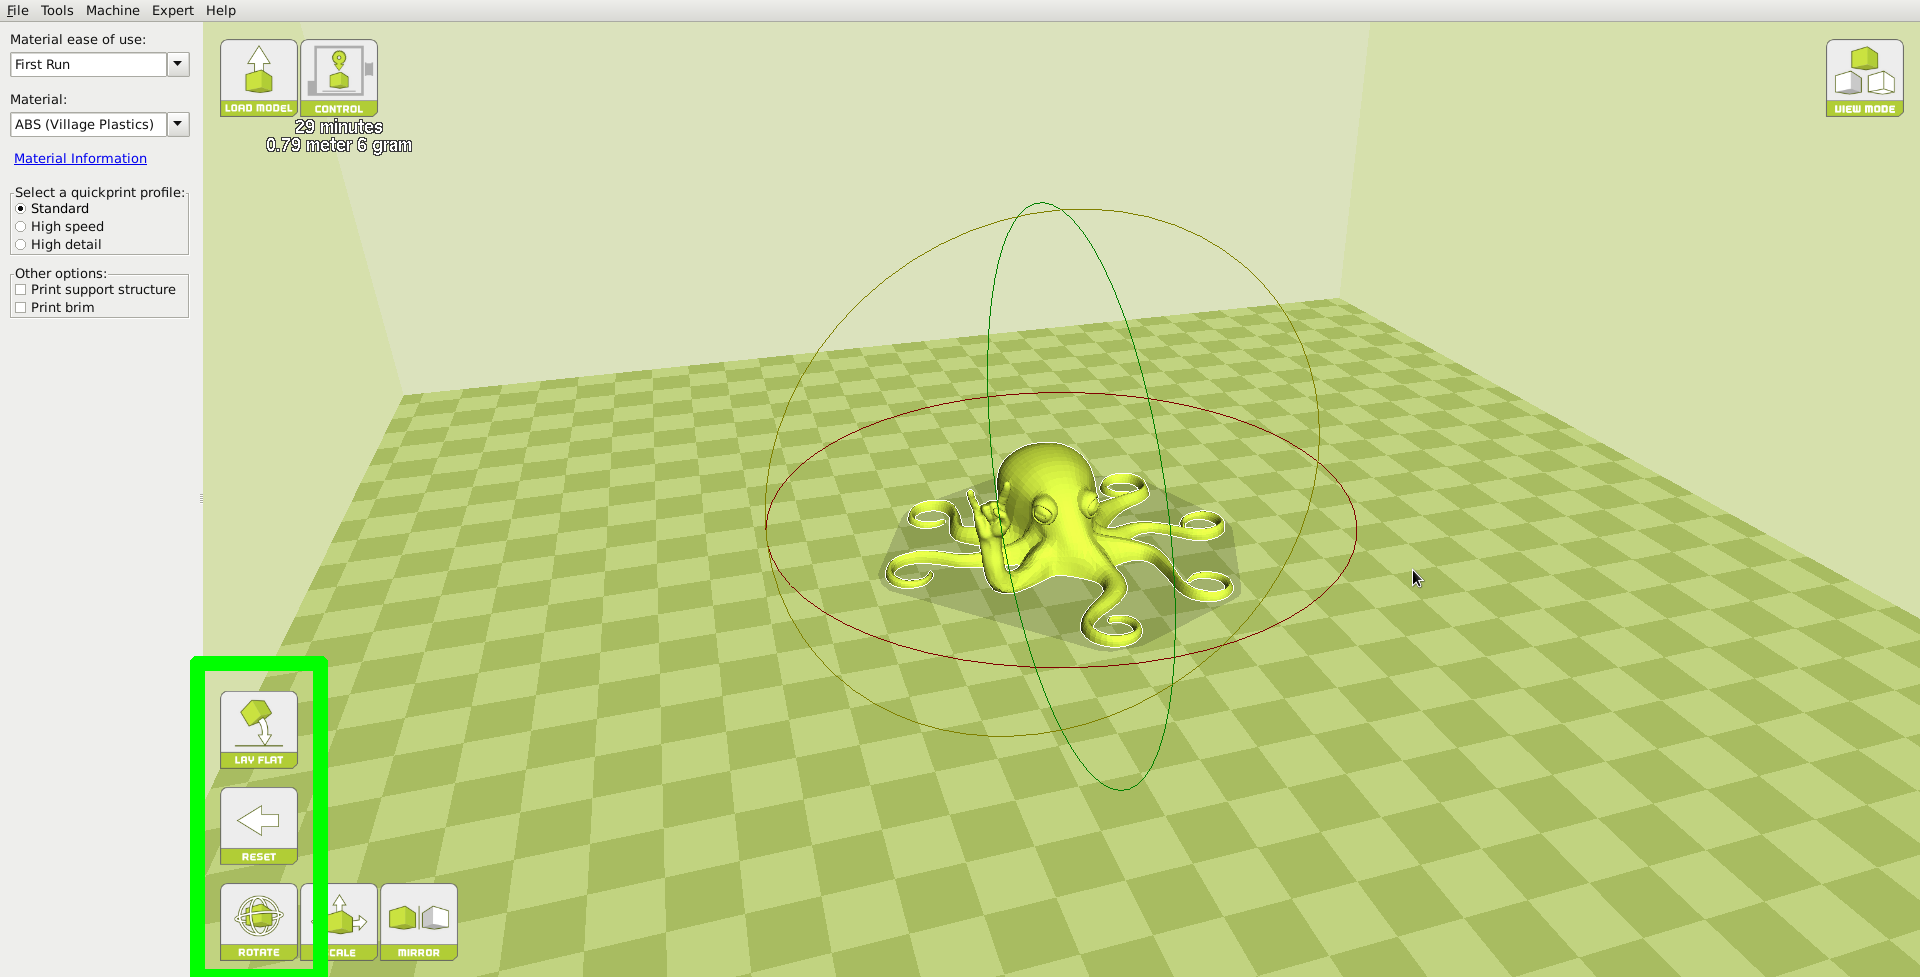
\includegraphics[keepaspectratio=true,angle=0,height=0.4\textheight,width=1.0\textwidth]{rotateTAZ.png}
\caption{Rotating your Model}
\label{fig:Rotating your Model}
\end{figure}

\subsubsection{Lay Flat}
The \texttt{Lay Flat} button will ensure that the flat portion of your print is securely attached to the bed. It is highly recommended to use this option after rotating your model in the Z direction, as it will help prevent adhesion issues during the print.
%\begin{figure}[hbt]
%\centering
%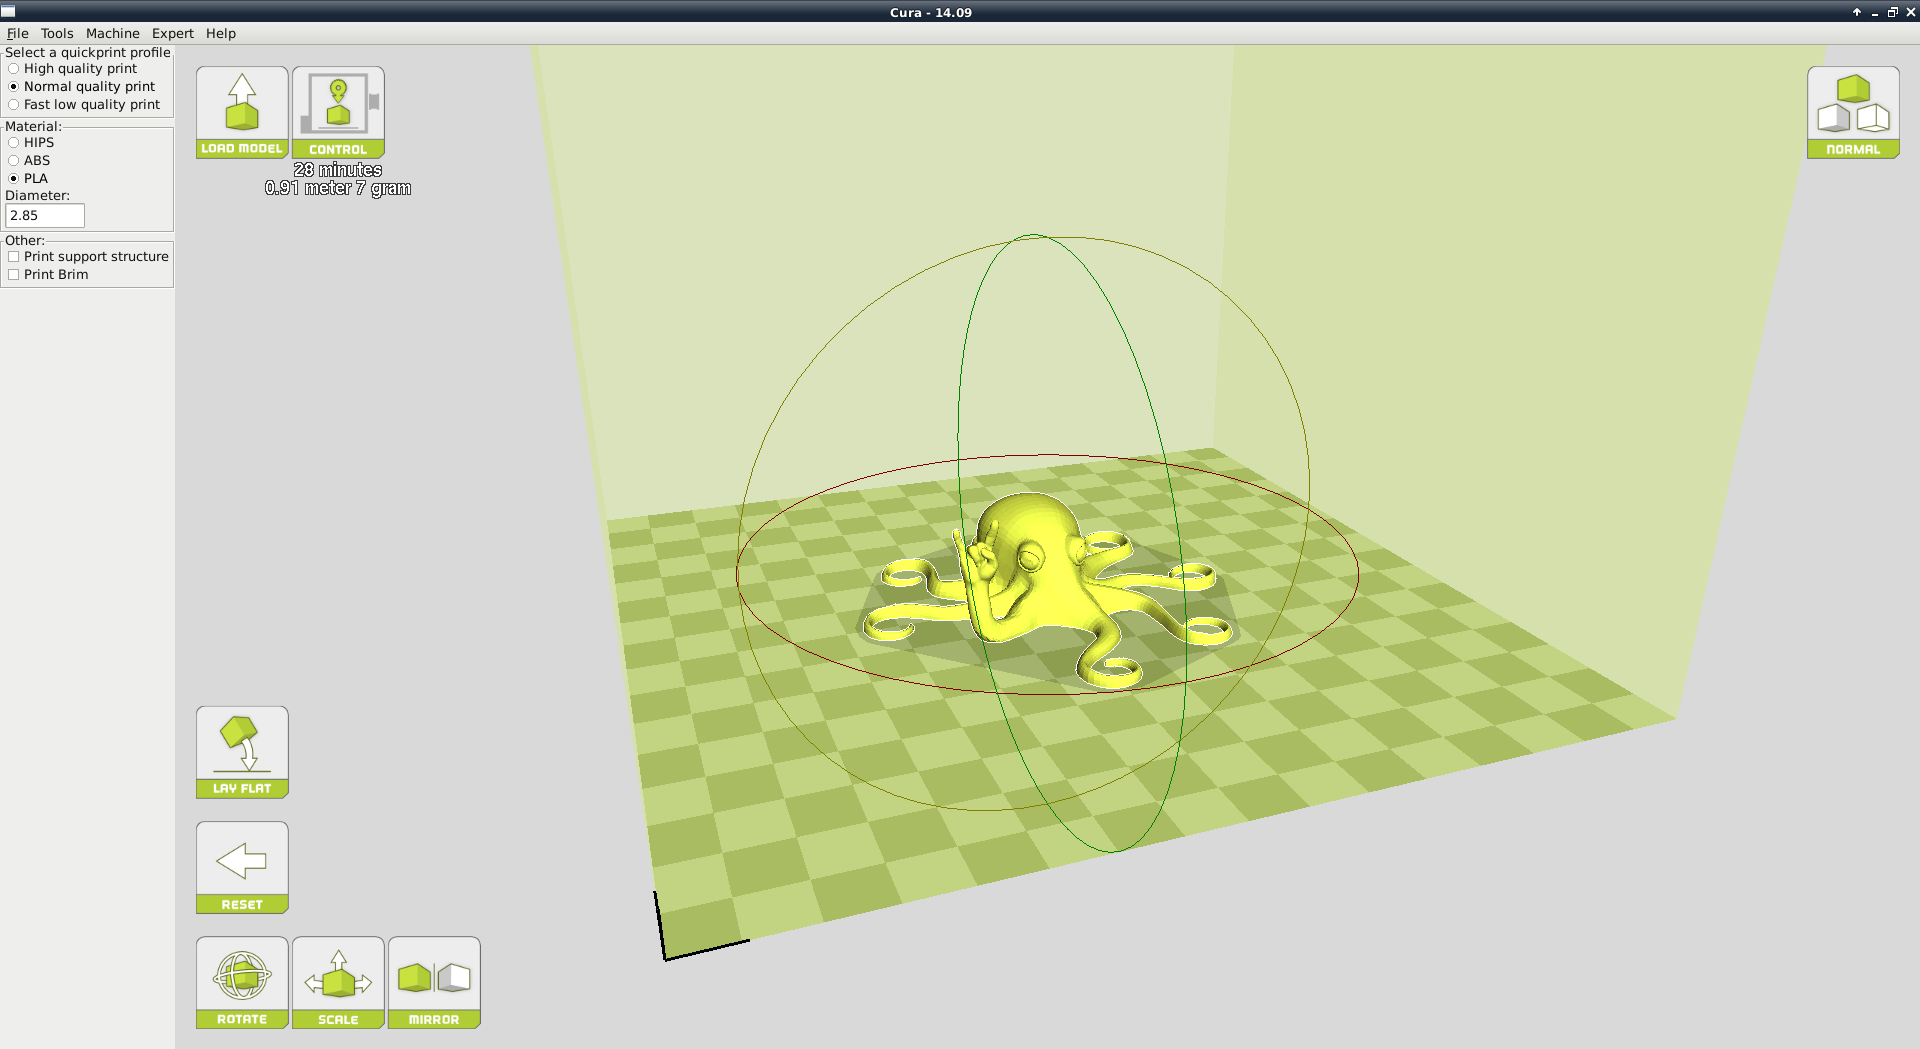
\includegraphics[keepaspectratio=true,angle=0,height=0.4\textheight,width=1.0\textwidth]{Rotate.png}
%\caption{Rotating your Model}
%\label{fig:Rotating your Model}
%\end{figure}

\subsubsection{Reset}
The \texttt{Reset} button will return your model to the original orientation as defined by the CAD program used to create the model.
%\begin{figure}[hbt]
%\centering
%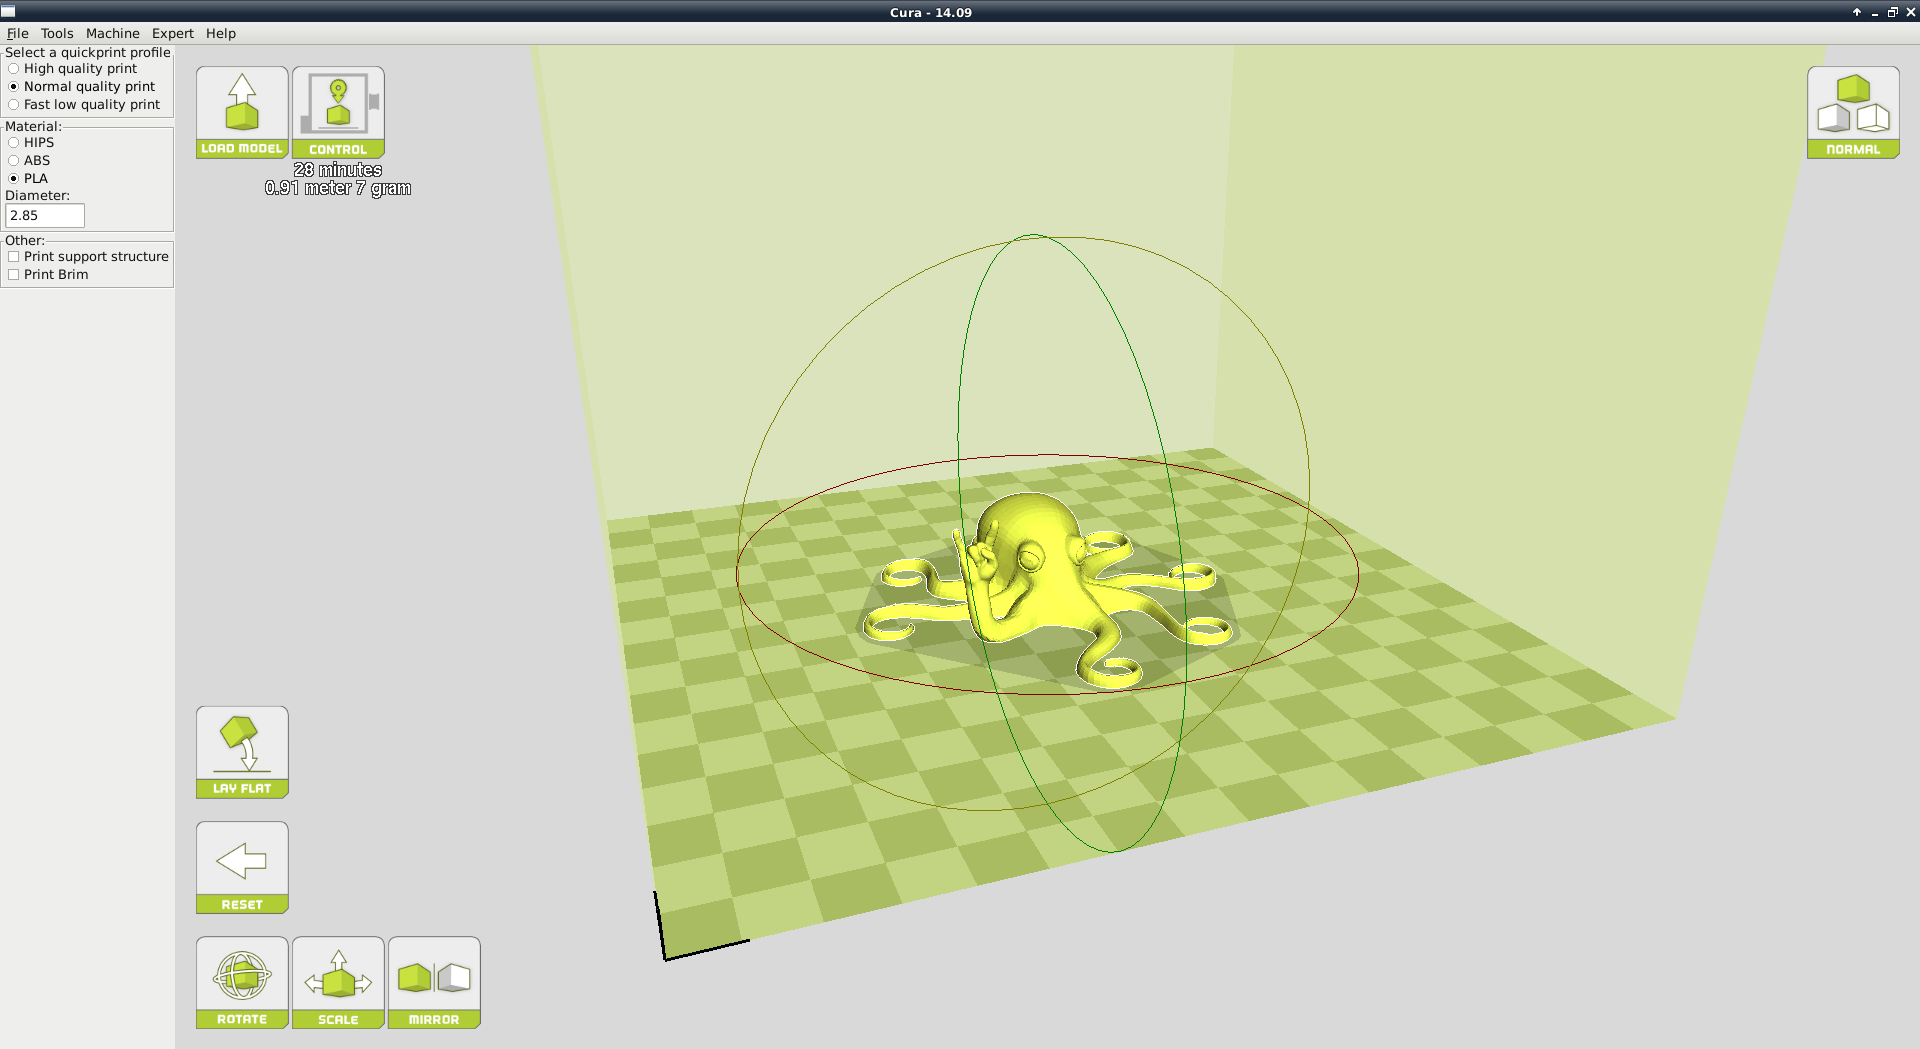
\includegraphics[keepaspectratio=true,angle=0,height=0.4\textheight,width=1.0\textwidth]{Rotate.png}
%\caption{Rotating your Model}
%\label{fig:Rotating your Model}
%\end{figure}

\subsubsection{Scale}
The \texttt{Scale} button displays the model dimensions, along with the ability to scale along the X Y or Z axes. Anything \texttt{below} the number \texttt{1.0} will reduce the objects size, while anything \texttt{above} the number \texttt{1.0} will increase the objects size. As a default, it will be set to uniform scaling. This will cause the X Y and Z axes to be scaled by the same amount when you make a change to any of them. To disable this, select the lock in the lower section of the scaling window. 
\begin{figure}[H]
\centering
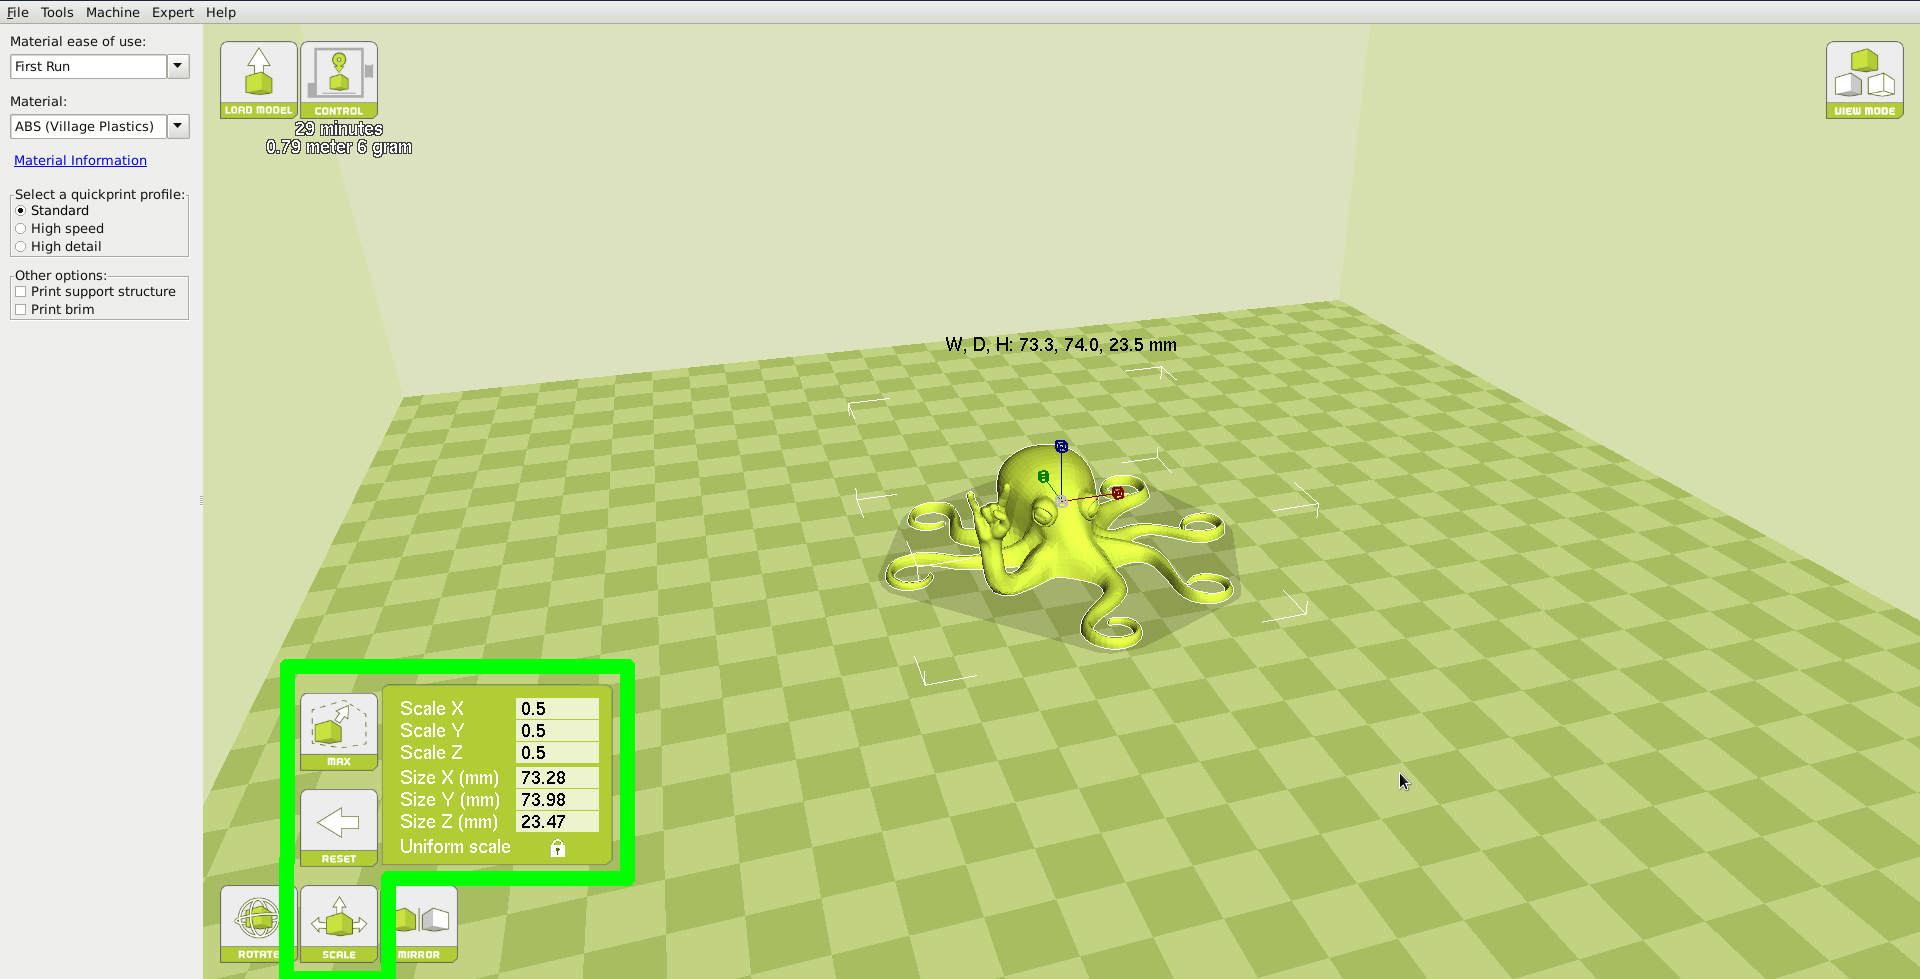
\includegraphics[keepaspectratio=true,angle=0,height=0.4\textheight,width=1.0\textwidth]{scaleTAZ.png}
\caption{Scaling your Model}
\label{fig:Scaling your Model}
\end{figure}

\section{View Options}
\index{View Options}
This mode allows you to view your model in a variety of different ways. This can be helpful for spotting issues before the print even starts. 

\subsection{Normal}
This is the standard view and shows the solid outer surfaces of the model. (Fig. \ref{fig:Normal View}, page \pageref{fig:Normal View}): 

\begin{figure}[H]
\centering
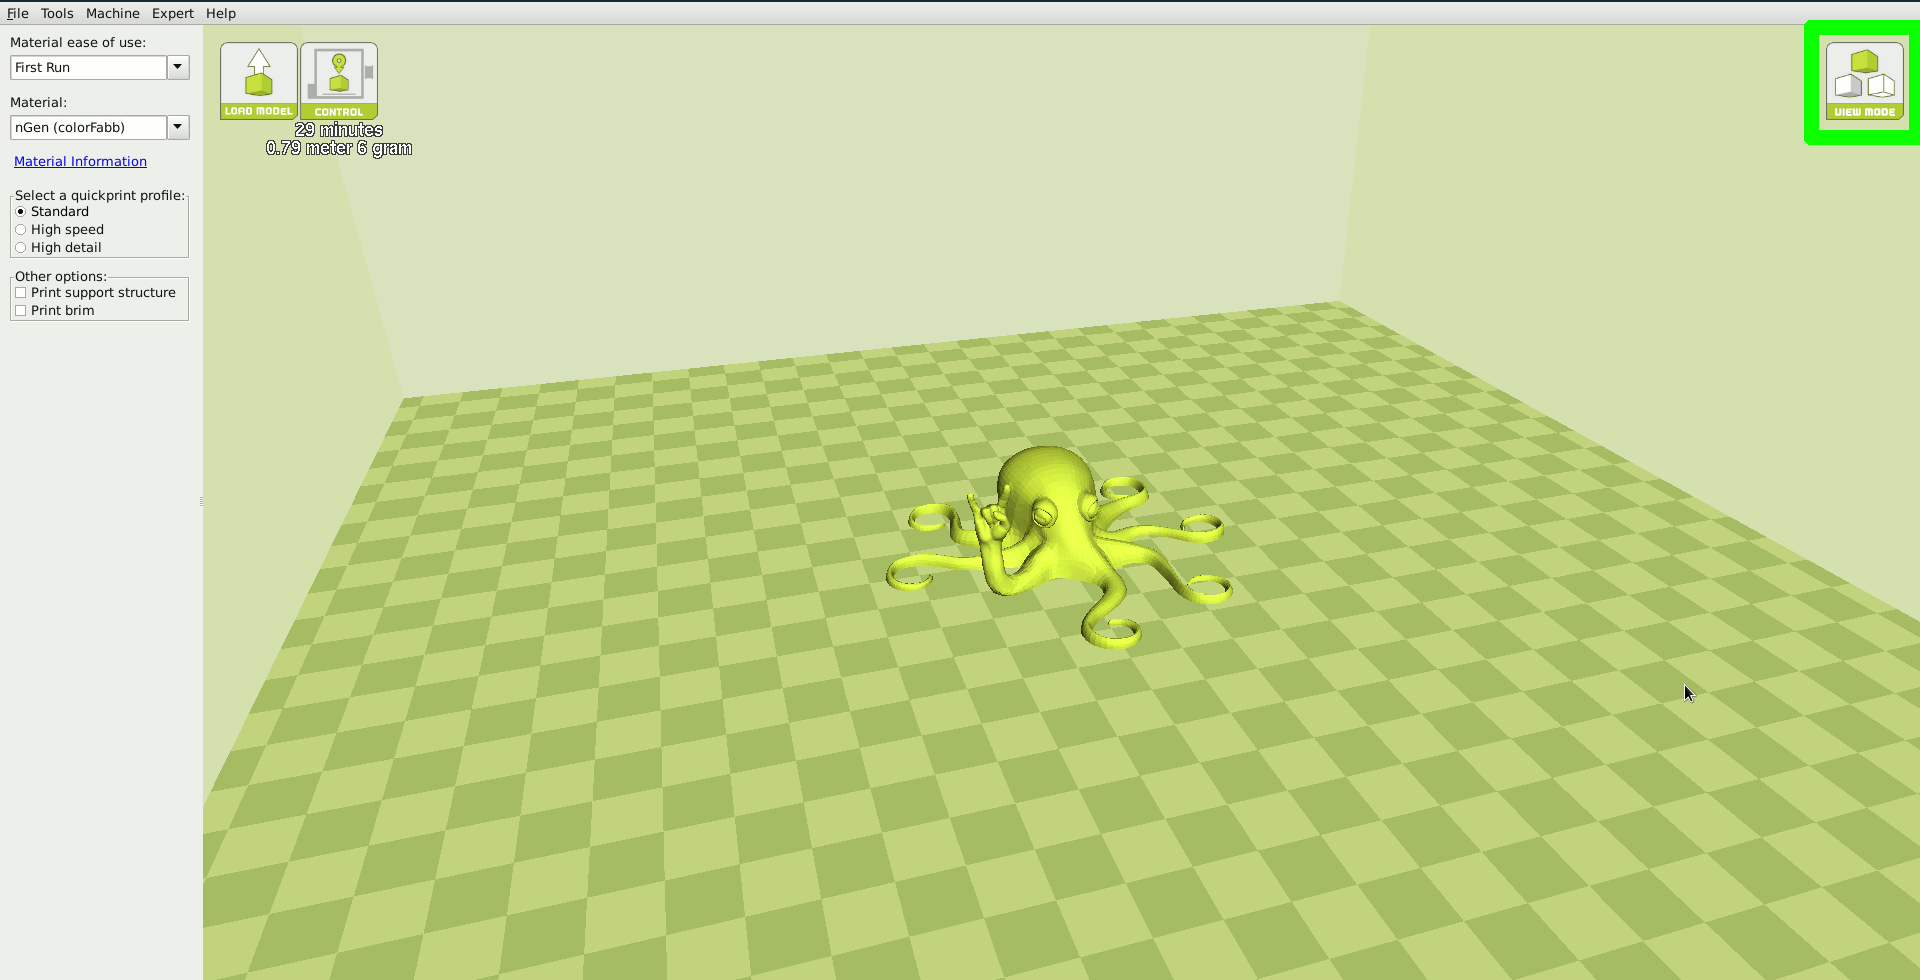
\includegraphics[keepaspectratio=true,angle=0,height=0.3\textheight,width=1.0\textwidth]{viewTAZ.png}
\caption{View in Normal Mode}
\label{fig:Normal View}
\end{figure}

\subsection{Overhang}
\index{Overhang} 
Overhang mode shows where your model may need support material. In Fig. \ref{fig:Overhang_View}, page \pageref{fig:Overhang_View} the red highlighted areas show overhangs and more severe angles and areas where support material is recommended. The overhang threshold can be defined in Expert Settings.
\begin{figure}[H]
\centering
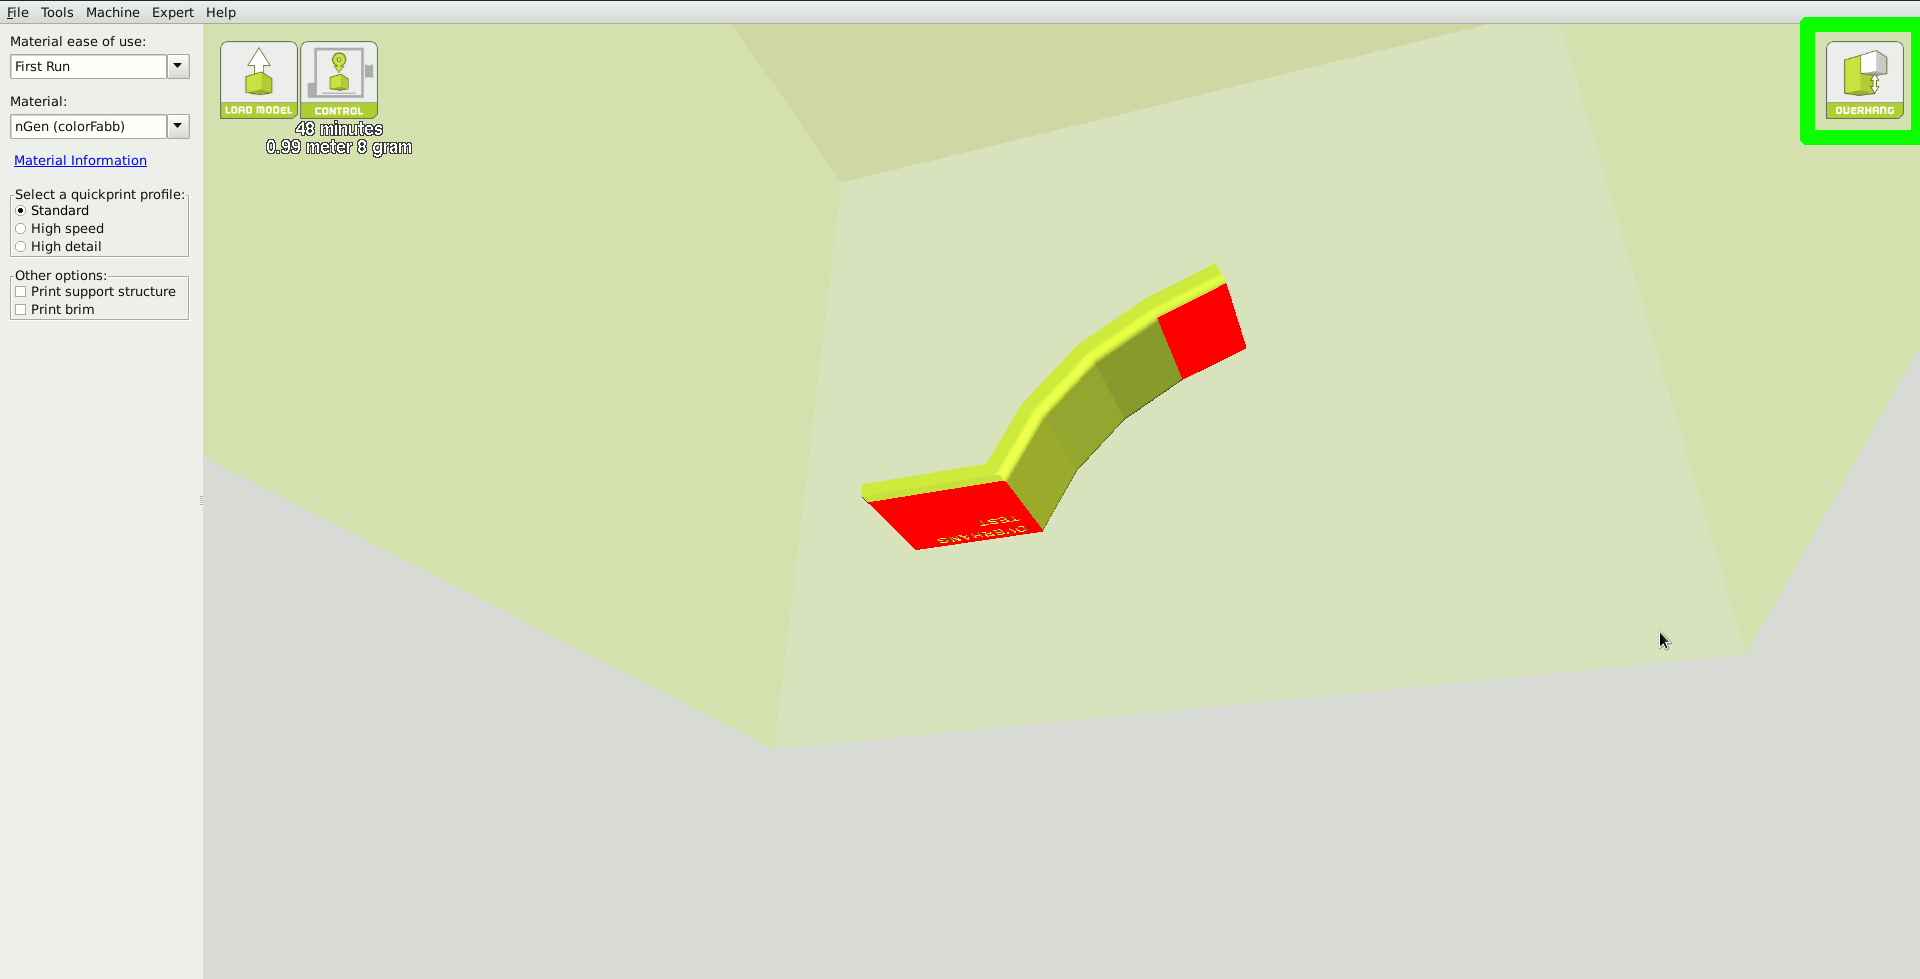
\includegraphics[keepaspectratio=true,angle=0,height=0.3\textheight,width=1.0\textwidth]{overhangTAZ.png}
\caption{View in Overhang}
\label{fig:Overhang_View}
\end{figure}

\subsection{Ghost}
\index{Ghost}
Ghost view mode makes the model translucent to allow you to see what is behind it.
\begin{figure}[H]
\centering
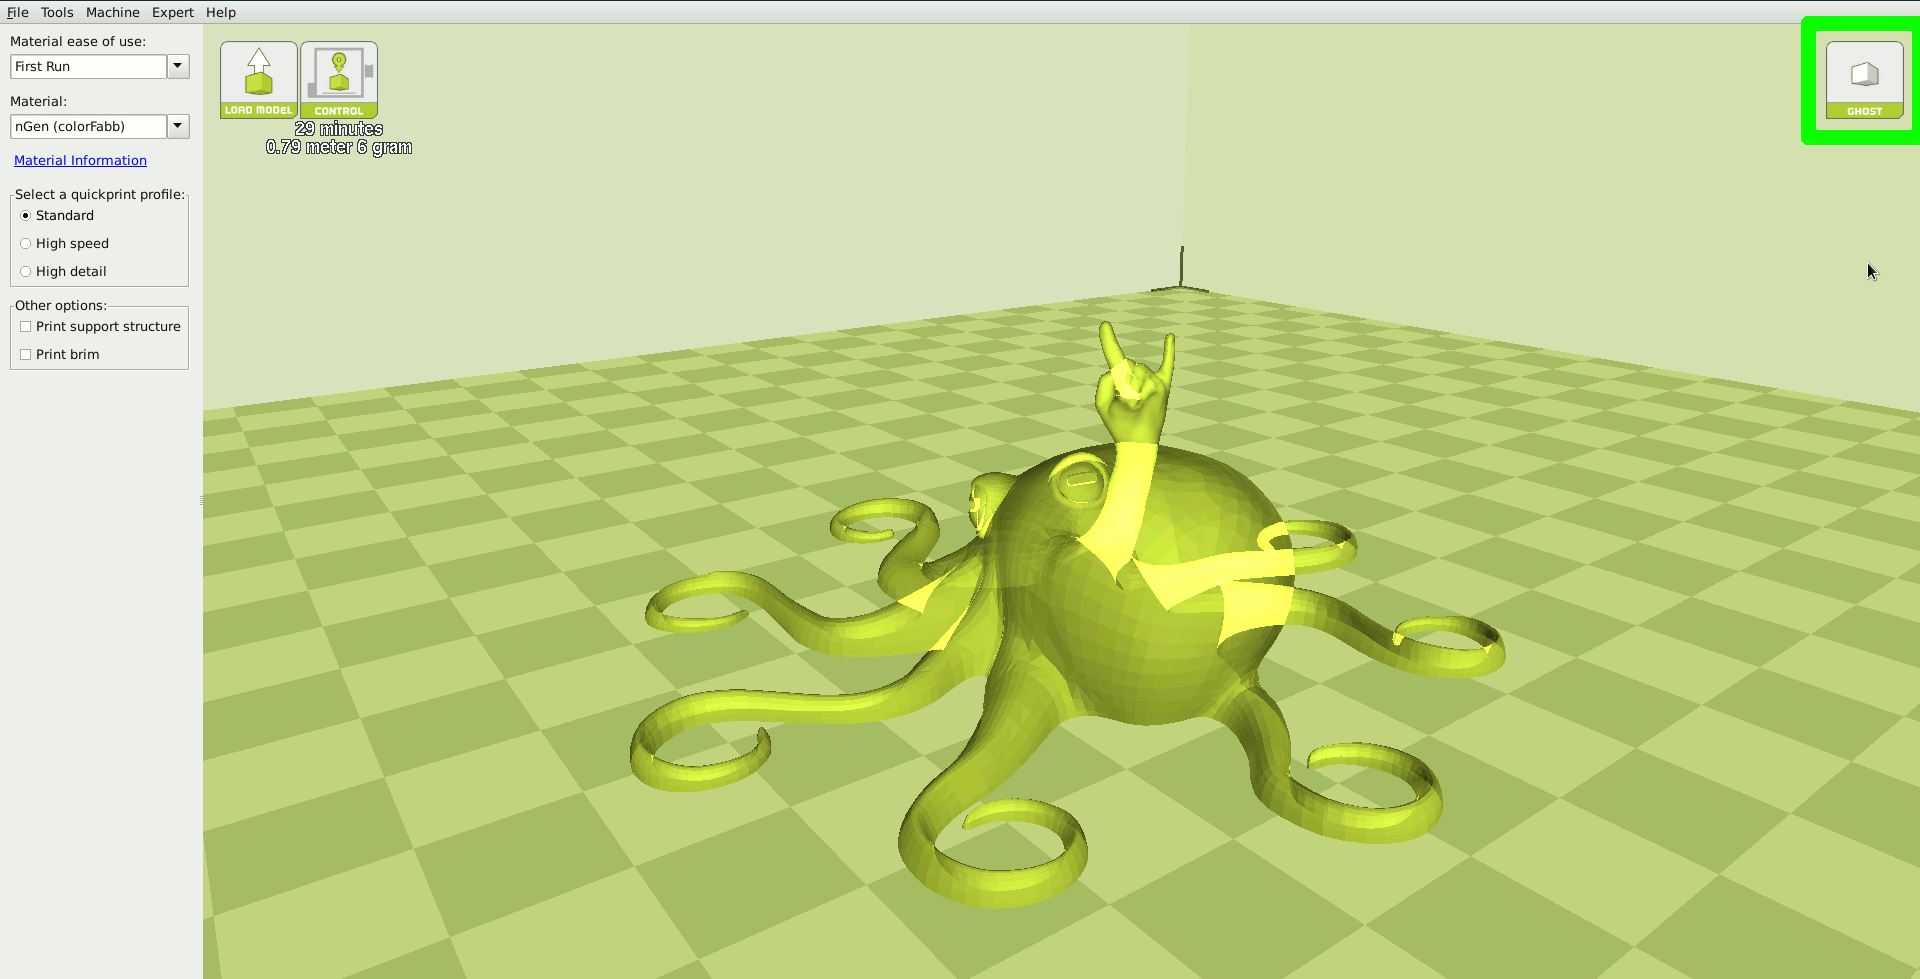
\includegraphics[keepaspectratio=true,angle=0,height=0.3\textheight,width=1.0\textwidth]{ghostTAZ.png}
\caption{View in Ghost}
\label{fig:Ghost View}
\end{figure}

\subsection{Xray}
\index{Xray}
Xray is very similar to Ghost mode. It will allow you to see into objects, ensuring that inner details are correct.
\begin{figure}[H]
\centering
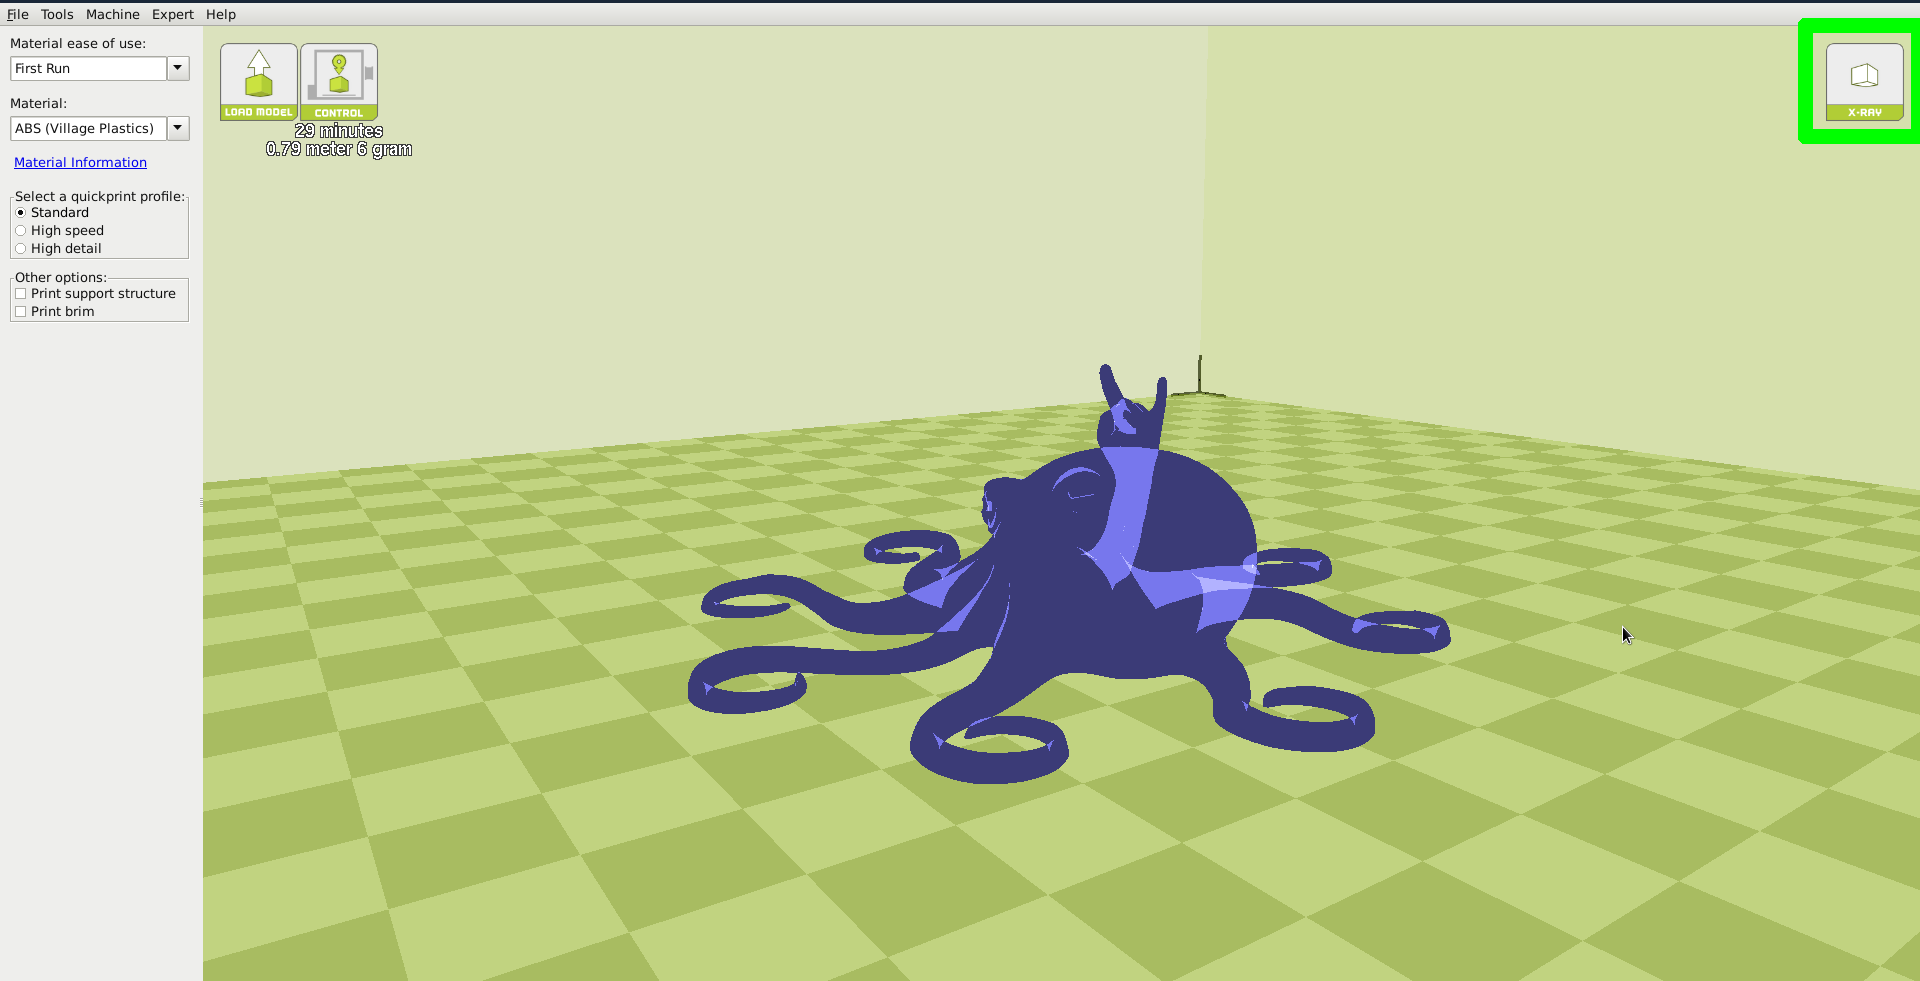
\includegraphics[keepaspectratio=true,angle=0,height=0.3\textheight,width=1.0\textwidth]{xrayTAZ.png}
\caption{View in Xray}
\label{fig:Xray View}
\end{figure}

\subsection{Layers}
\index{Layers}
To view the tool path of your print head and to ensure no skipped layers or gaps use this option. Use the slide bar on the right hand side of the window to move up and down through the tool path layers. Click the icon below it to view an individual layer at a time. If there is support activated in your model, it will be shown in blue.
\begin{figure}[H]
\centering
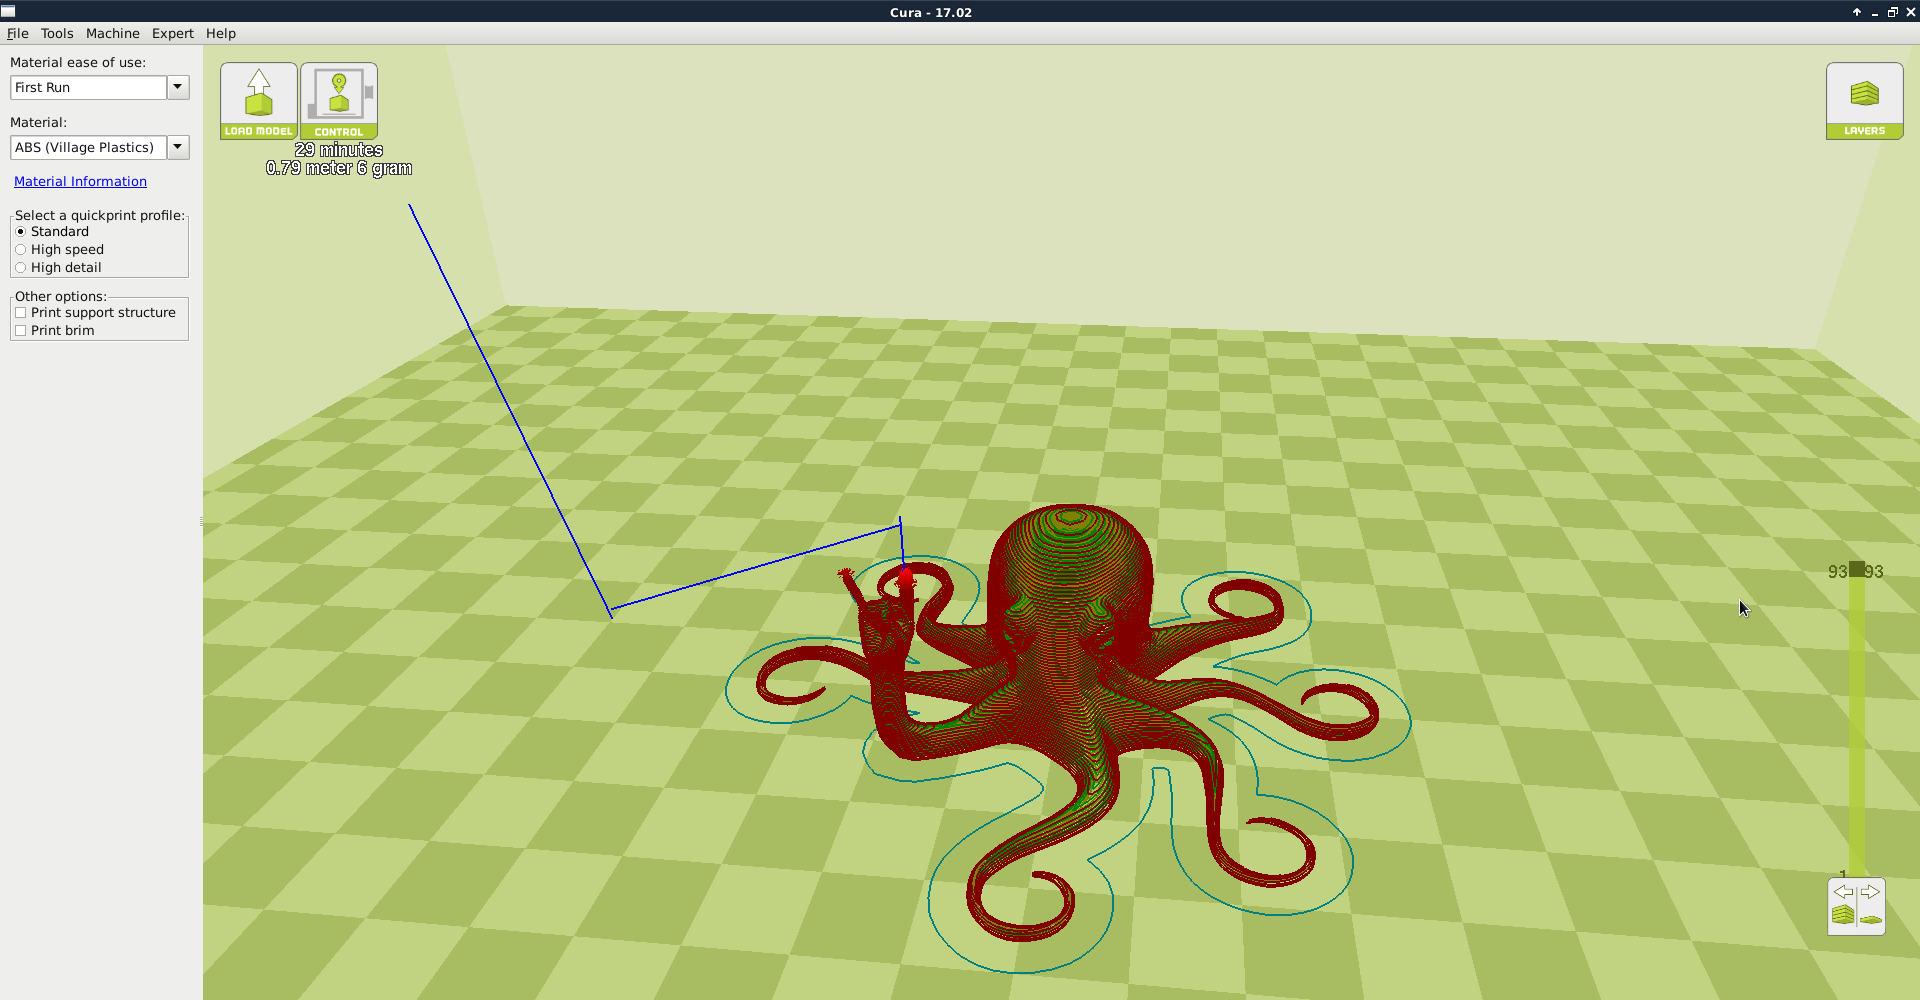
\includegraphics[keepaspectratio=true,angle=0,height=0.3\textheight,width=1.0\textwidth]{layersTAZ.png}
\caption{View in Layers}
\label{fig:Layers View}
\end{figure}

\begin{figure}[H]
\centering
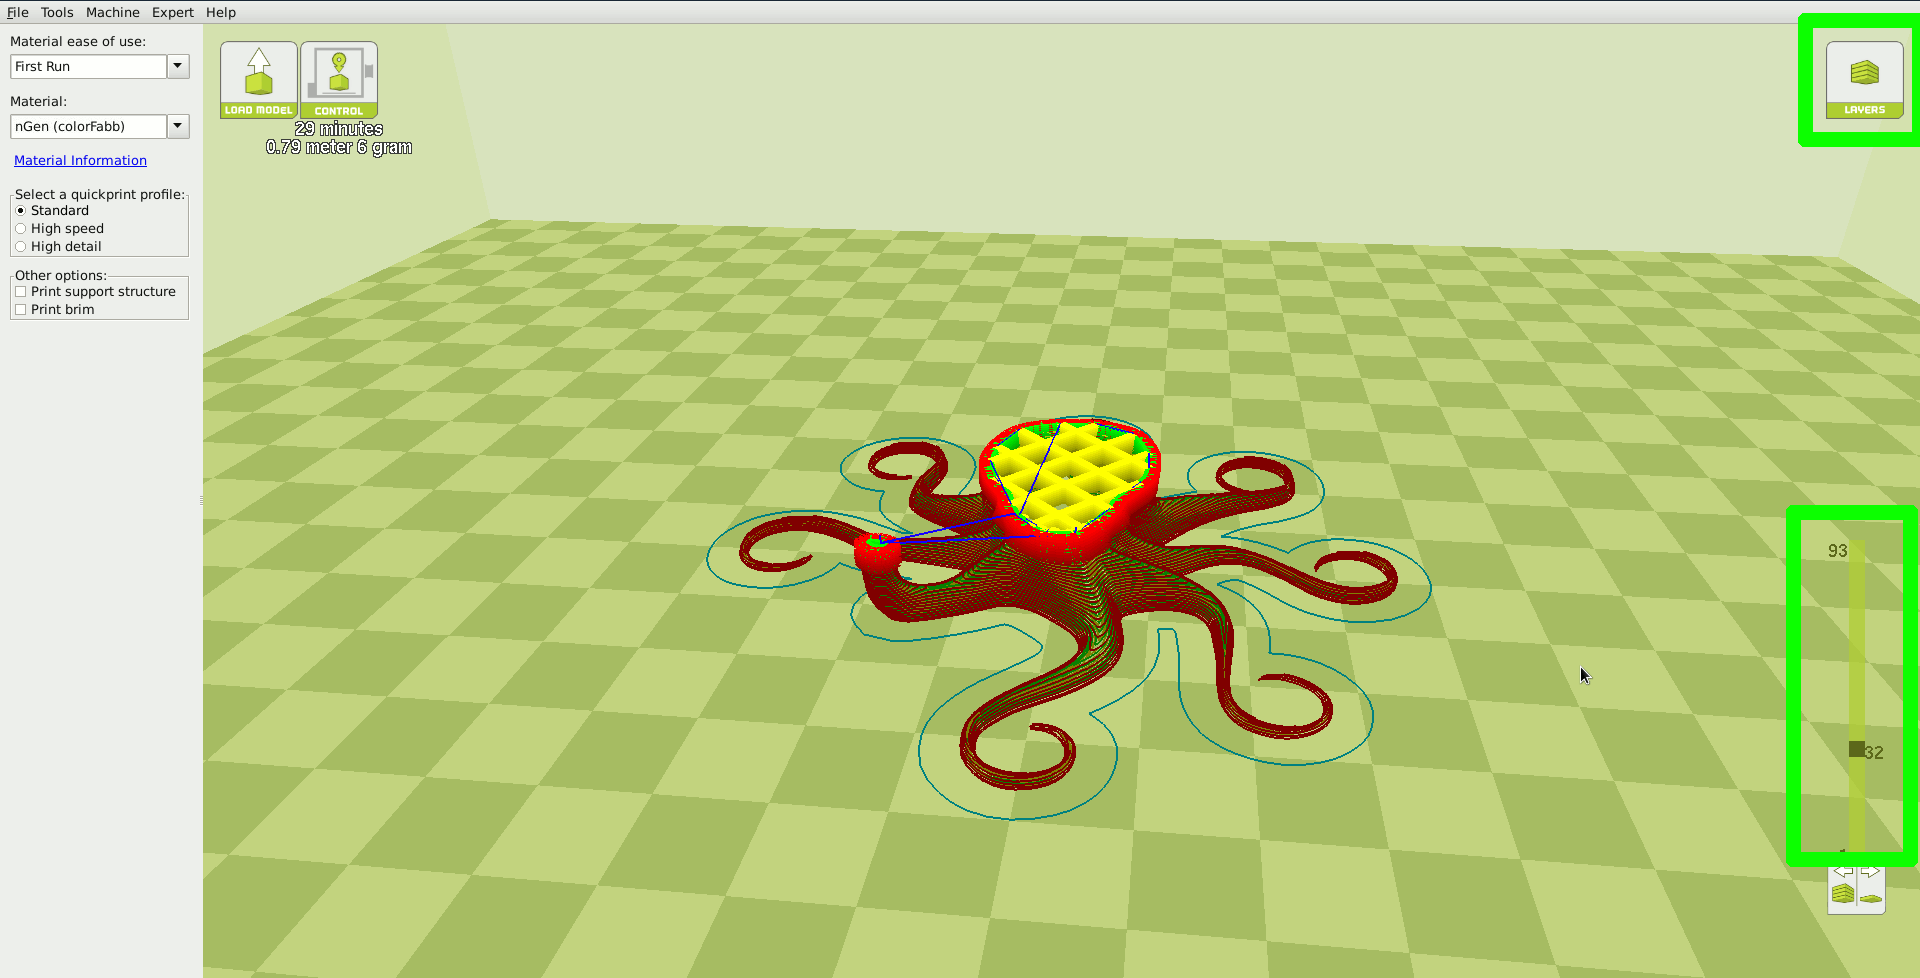
\includegraphics[keepaspectratio=true,angle=0,height=0.3\textheight,width=1.0\textwidth]{cumulativeTAZ.png}
\caption{Viewing Cumulative Layers}
\label{fig:Mid Layers View}
\end{figure}

\begin{figure}[H]
\centering
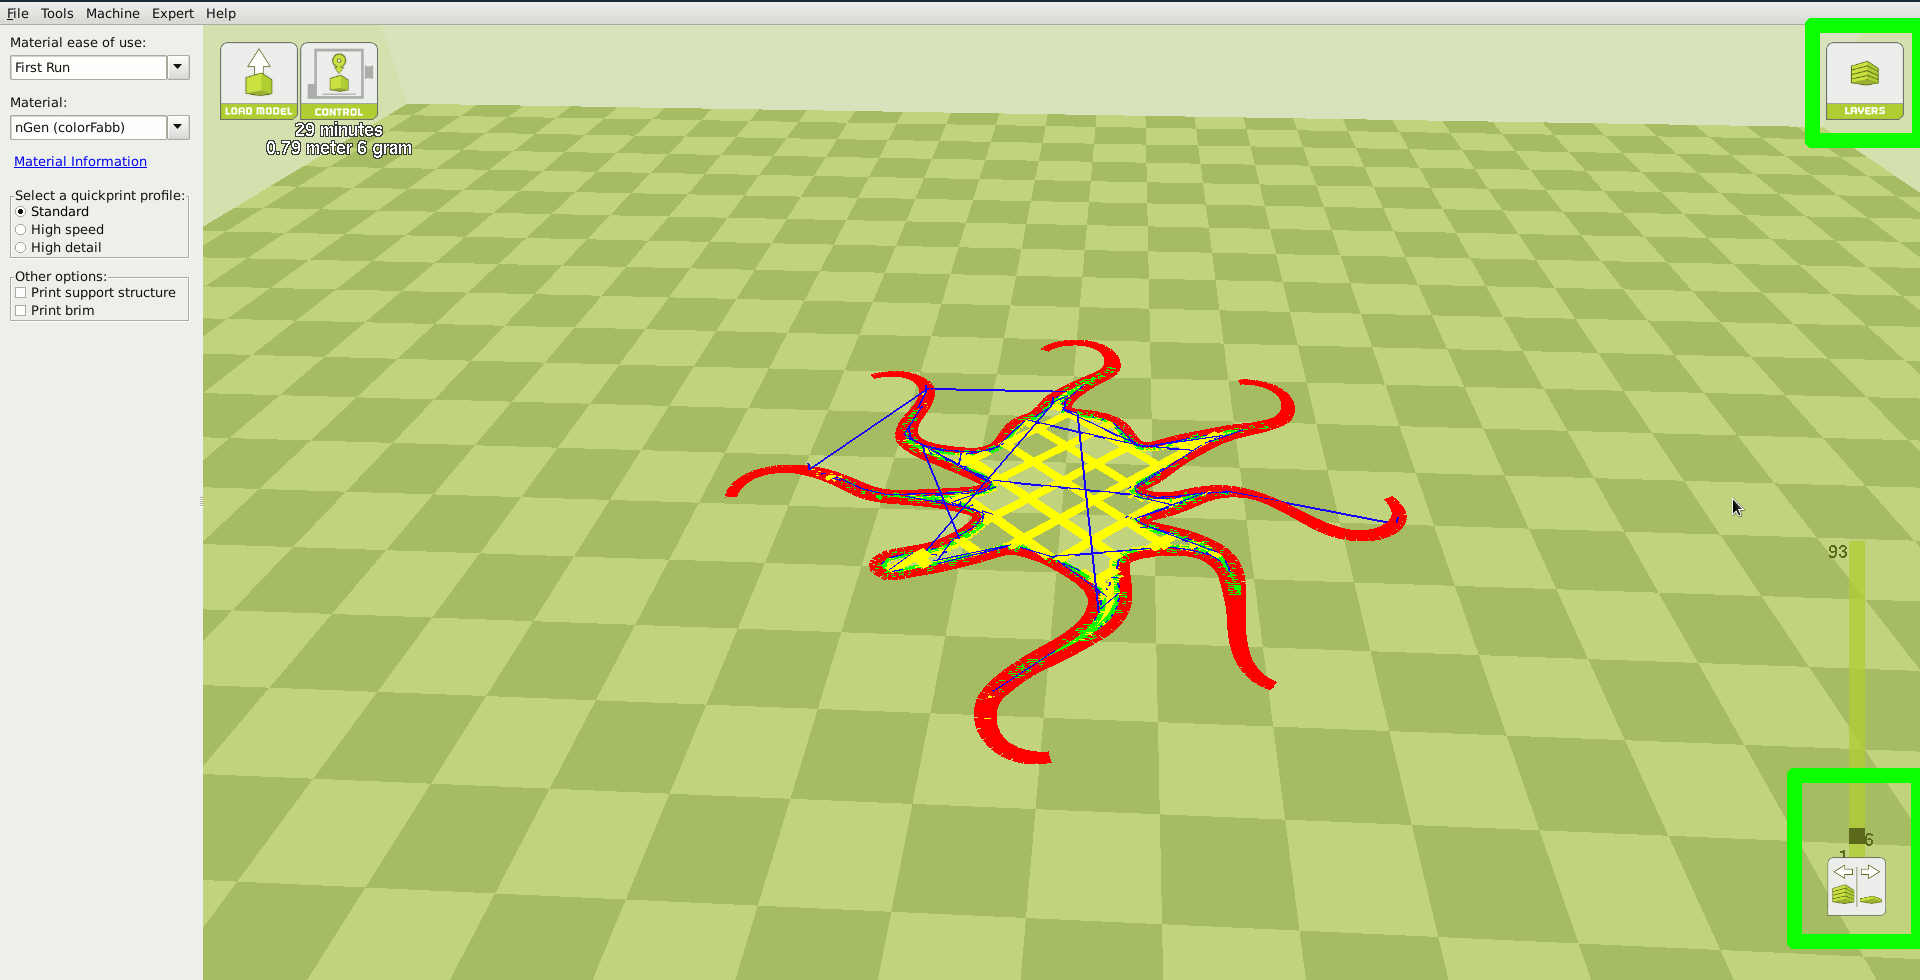
\includegraphics[keepaspectratio=true,angle=0,height=0.3\textheight,width=1.0\textwidth]{individualTAZ.png}
\caption{Viewing Specific Layers}
\label{fig:Viewing Specific Layer}
\end{figure}

\section{Starting Your First Print}
\index{First Print}
Once you have your model, profile, and filament loaded, it is time for your first print! 


%\subsection{Mini}

%Select the \texttt{Print/Control} option in the top left hand corner of your build volume. This will bring up your Printer Interface. Please wait for the window title to display \texttt{operational} before sending any commands to the printer..

%\pageref{fig:Print Control}).
%\begin{figure}[hbt]
%\centering
%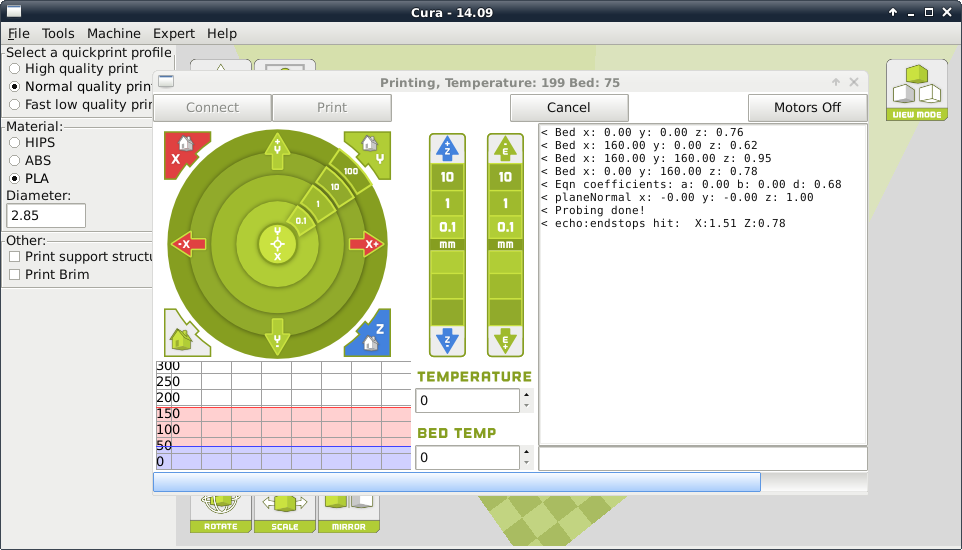
\includegraphics[keepaspectratio=true,angle=0,height=0.4\textheight,width=1.0\textwidth]{print_control.png}
%\caption{Print Control Screen}
%\label{fig:Print Control}
%\end{figure}

%\subsection{TAZ}

Your TAZ 3D printer has the ability to print directly from a computer using the included USB cable, or directly from the SD card by using the Graphical LCD controller.

%%%% SD Printing %%%%
\subsection{Printing from SD Card}
\index{Printing from SD}
\index{Graphical LCD controller}
\index{GLCD}
\index{SD card}
\index{SD}

Insert the included SD card into your computer. Select \texttt{File} > \texttt{Save Gcode} and choose the SD card location to save your Gcode file to your SD card. Insert the SD Card into the Graphical LCD Controller. 

\subsection{Set Temperature}

Turn on the heated bed and hot end by using the Graphical LCD controller and navigating to: \texttt{Temperature} > \texttt{Select Filament type}. If you are using other materials you can set your desired temperatures by going to \texttt{Temperature} > \texttt{Custom Temp} > \texttt{Nozzle/Bed}. Wait for your 3D printer to reach specified temperatures.

\subsection{Start Print}
\index{printing}
Once at the desired printing temperature begin your print through your Graphical LCD controller by navigating to: \texttt{Print From SD} > \texttt{Desired File}.

%%%% Tethered printing %%%%

\subsubsection{Printing from USB Cable}
\index{Printing from USB}

Connect your 3D printer to a computer using a USB cable, power it on and select the \texttt{Control} button at the top of the 3D viewing window. This will bring up your Pronterface user interface. You will not be able to send any commands until the window title changes to \texttt{Operational}. Once it is operational, you will need to set your filament specific temperatures. The temperature box heats the hot end, while the bed temp sets the bed temperature. Your current temperatures will be listed in the top of the control box. Once your hot end and bed are heated, select \texttt{Print}. This will start the printing process.

\begin{figure}[H]
\centering
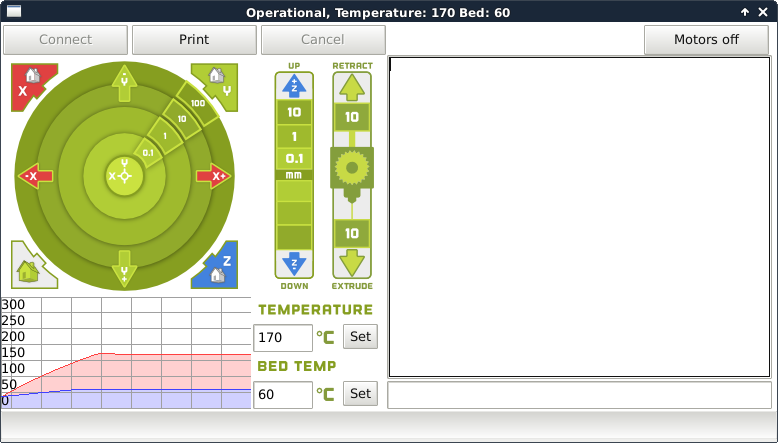
\includegraphics[keepaspectratio=true,angle=0,height=0.4\textheight,width=1.0\textwidth]{Pronterface117.png}
\caption{Control Screen}
\label{fig:Control}
\end{figure}

%\subsection{Pausing Mid-print}
%\index{Pause}
%You will notice after starting your print, the print button has changed to a pause button. This will pause your print after it has run through its Gcode buffer. Cura will remember the location of your print heads X and Y coordinates if moved through Cura. This allows you to move the print head away from your print and change filaments, colors, etc. When you hit resume, Cura will bring the print head back to the original (X,Y) before resuming. Disabling the motors, and manually moving the print head will cause Cura to lose the (X,Y) positioning. \textcolor{red}{Cura will NOT remember any Z movements}. If you would like to move in the Z direction, be sure to make the opposite movement before resuming.

\subsection{Recommended Temperatures}
\index{Temperatures}
When preparing your printer for operation, please be sure to set your temperatures, in Celsius, to the specific filament you are using. 
\begin{center}
 \hspace*{-1.5cm}\begin{tabular}{||c c c c c||} 
 \hline
 Filament Type & Bed Preparation & Nozzle Temp & Bed Temp & Removal Temp \\ [0.5ex] 
 \hline\hline
 ABS & Clean PEI & 240-260 & 110 & 50 \\ 
 \hline
 PLA & Clean PEI & 195-215 & 60 & 45 \\
 \hline
 HIPS & Clean PEI & 240-260 & 110 & 50\\
 \hline
 Laywoo-D3 & Clean PEI & 175-195 & 60 & 45 \\
 \hline
 Laybrick & Clean PEI & 175-195 & 60 & 45 \\
 \hline 
 Magnetic Iron PLA & Clean PEI & 220-230 & 60 & 45 \\
 \hline
 Stainless Steel PLA & Clean PEI & 220-230 & 60 & 45 \\
 \hline
 t-glase & Glue stick & 240-260 & 60 & 45 \\
 \hline
 Flexible Filaments & Glue stick & 215-230 & 50 & 35 \\  
 \hline
 Nylons & Glue stick & 220-270 & 110 & 50 \\
 \hline
 Polycarbonate & Glue stick & 260-300 & 110 & 50 \\ 
 \hline
 Polycarbonate + ABS & Glue stick & 260-280 & 110 & 50 \\
 \hline 
 Conductive PLA & Clean PEI & 215-230 & 60 & 50 \\
 \hline
 N-Vent & Glue stick & 220-260 & 110 & 50 \\ [1ex]
 \hline
 
\end{tabular}
\end{center}

%%mini:
%This will start the printing process: (set the appropriate temperatures, go through the auto-leveling procedure, and start printing your model).
%\pageref{fig:Print Control}).


\section{Removing Your First Print}
\index{Removing a Print}
After your first print has finished, you need to wait for the part to cool down.  Your parts will be easier to remove if you allow your heated bed to cool down to optimal temperature. This will allow the plastic to contract, making it easier to remove. 
%\texttt{Your print bed will move forward once it is ready to be removed.}

Once your heated bed has cooled, use the blue handled knife that was included with your toolkit to remove the item. Carefully insert the blade of the knife between your print and heated bed. Once underneath the part rotate the blade lifting with the sharp edge into the part, to gently pop the piece off your plate.
%\begin{figure}[hbt]
%\centering
%\includegraphics[keepaspectratio=true,angle=0,height=0.4\textheight,width=1.0\textwidth]{remove_part.png} %%%% Photo needed %%%%
%\caption{Remove Part}
%\label{fig:Remove part}
%\end{figure}

\section{Full Settings}
\index{Full Settings}
\textcolor{red}{Full settings should not be used until enough experience with 3D printing has been gained to feel comfortable with all aspects of the printer and its operation. The Quickprint Mode will provide good results for most models.}
The first time Cura is launched it will default to the \texttt{Quick Print} interface. In order to have more control of your slicing and Gcode generation, switch to \texttt{Full Settings}. Select \texttt{Expert} > \texttt{Switch to full settings}. If a quickprint profile for your filament type is available, be sure to have it selected. This will automatically update the settings for that filament. The following tabs will now be available: Basic, Advanced, Plugins, and Start/End-Gcode. You will also have access to the Expert Settings. 
%\begin{figure}[H]
%\centering
%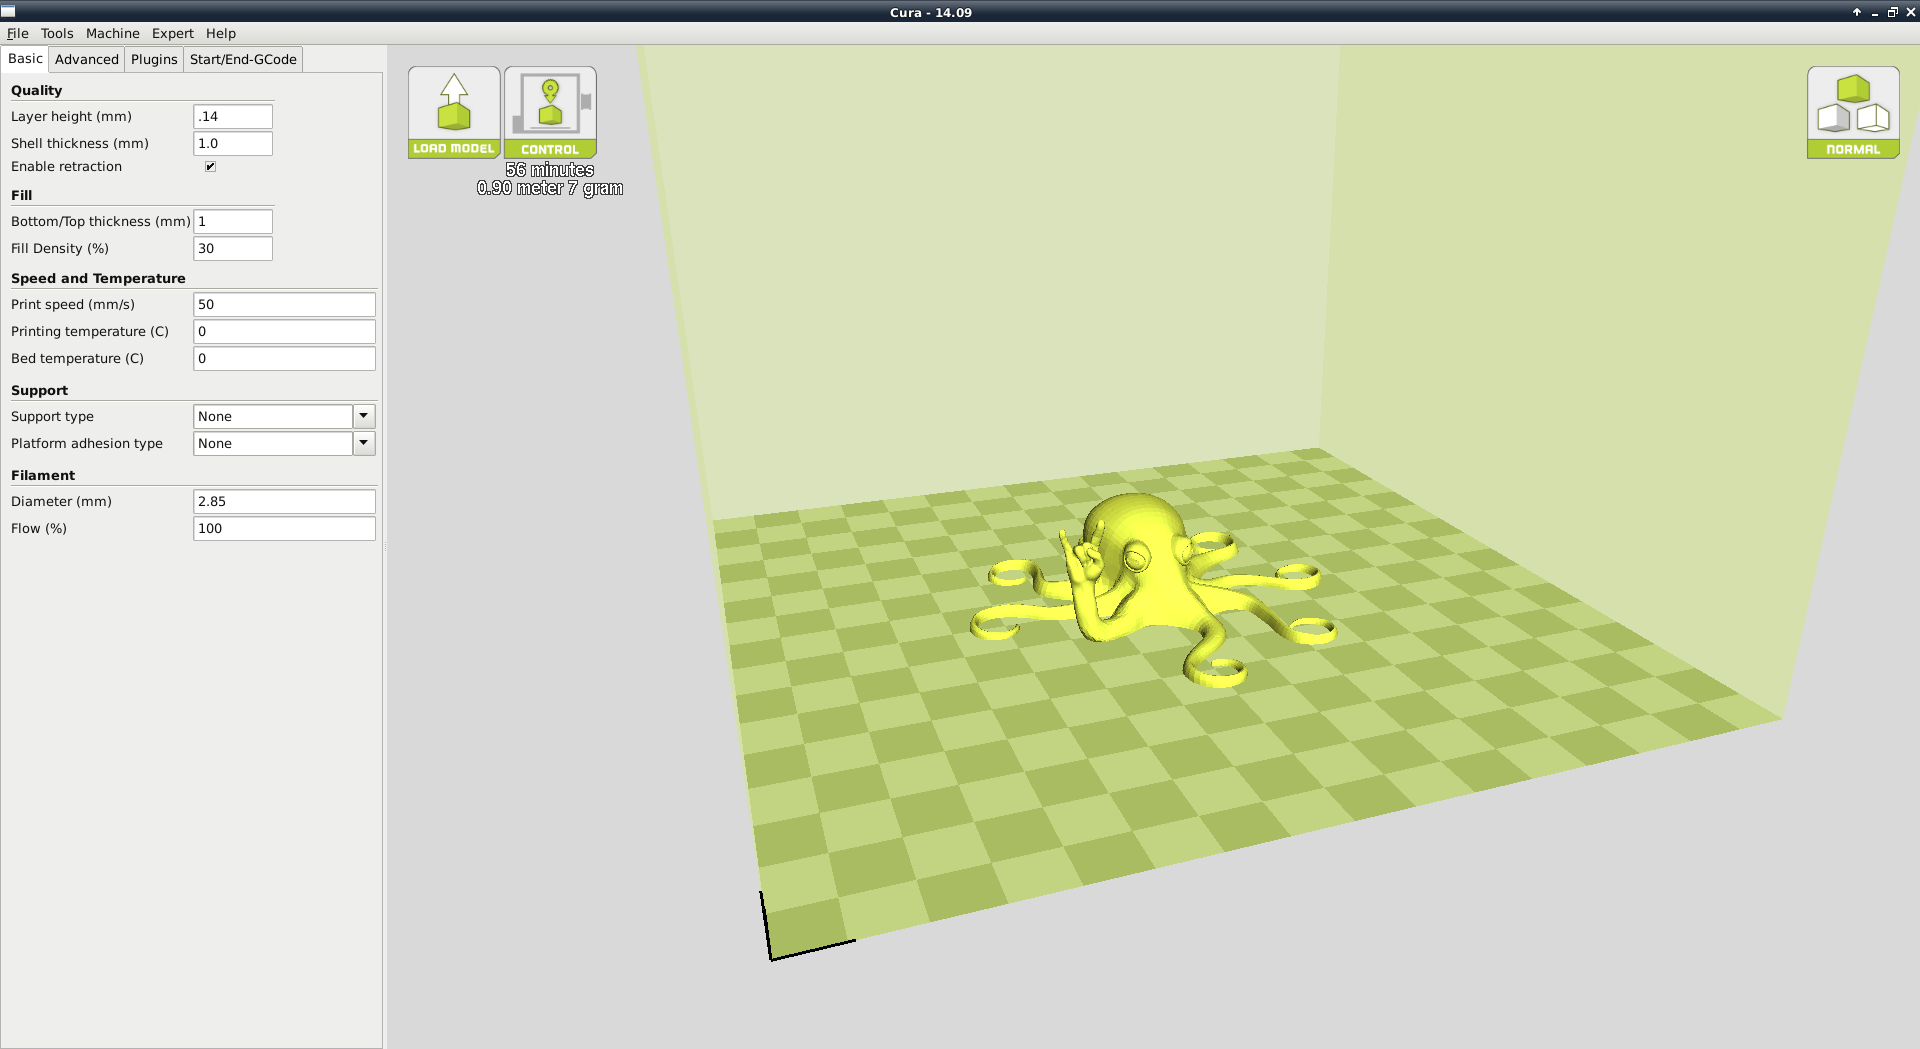
\includegraphics[keepaspectratio=true,angle=0,height=0.4\textheight,width=1.0\textwidth]{Expert.png}
%\caption{View in Full Settings}
%\label{fig:Full Settings View}
%\end{figure}

\subsection{View in Full Settings}
\index{Full Settings}
When you first switch to Full Settings, Cura will need to know what filament and quality you wish to use. It will automatically transfer our quickprint settings over to allow adjustments if one is selected. \textcolor{red}{IF A QUICKPRINT PROFILE IS NOT AVAILABLE, YOU WILL NEED TO MANUALLY LOAD ONE IN.} We recommend using our tested profiles that are available here: \texttt{https://www.lulzbot.com/cura}. You will want to choose the profile that matches your filament and quality needs. Once downloaded, you can load the file into Cura by selecting \texttt{File} > \texttt{Open Profile}. Choose your desired profile. This will automatically update all of your settings for use with your printer.
\begin{figure}[hbt]
\centering
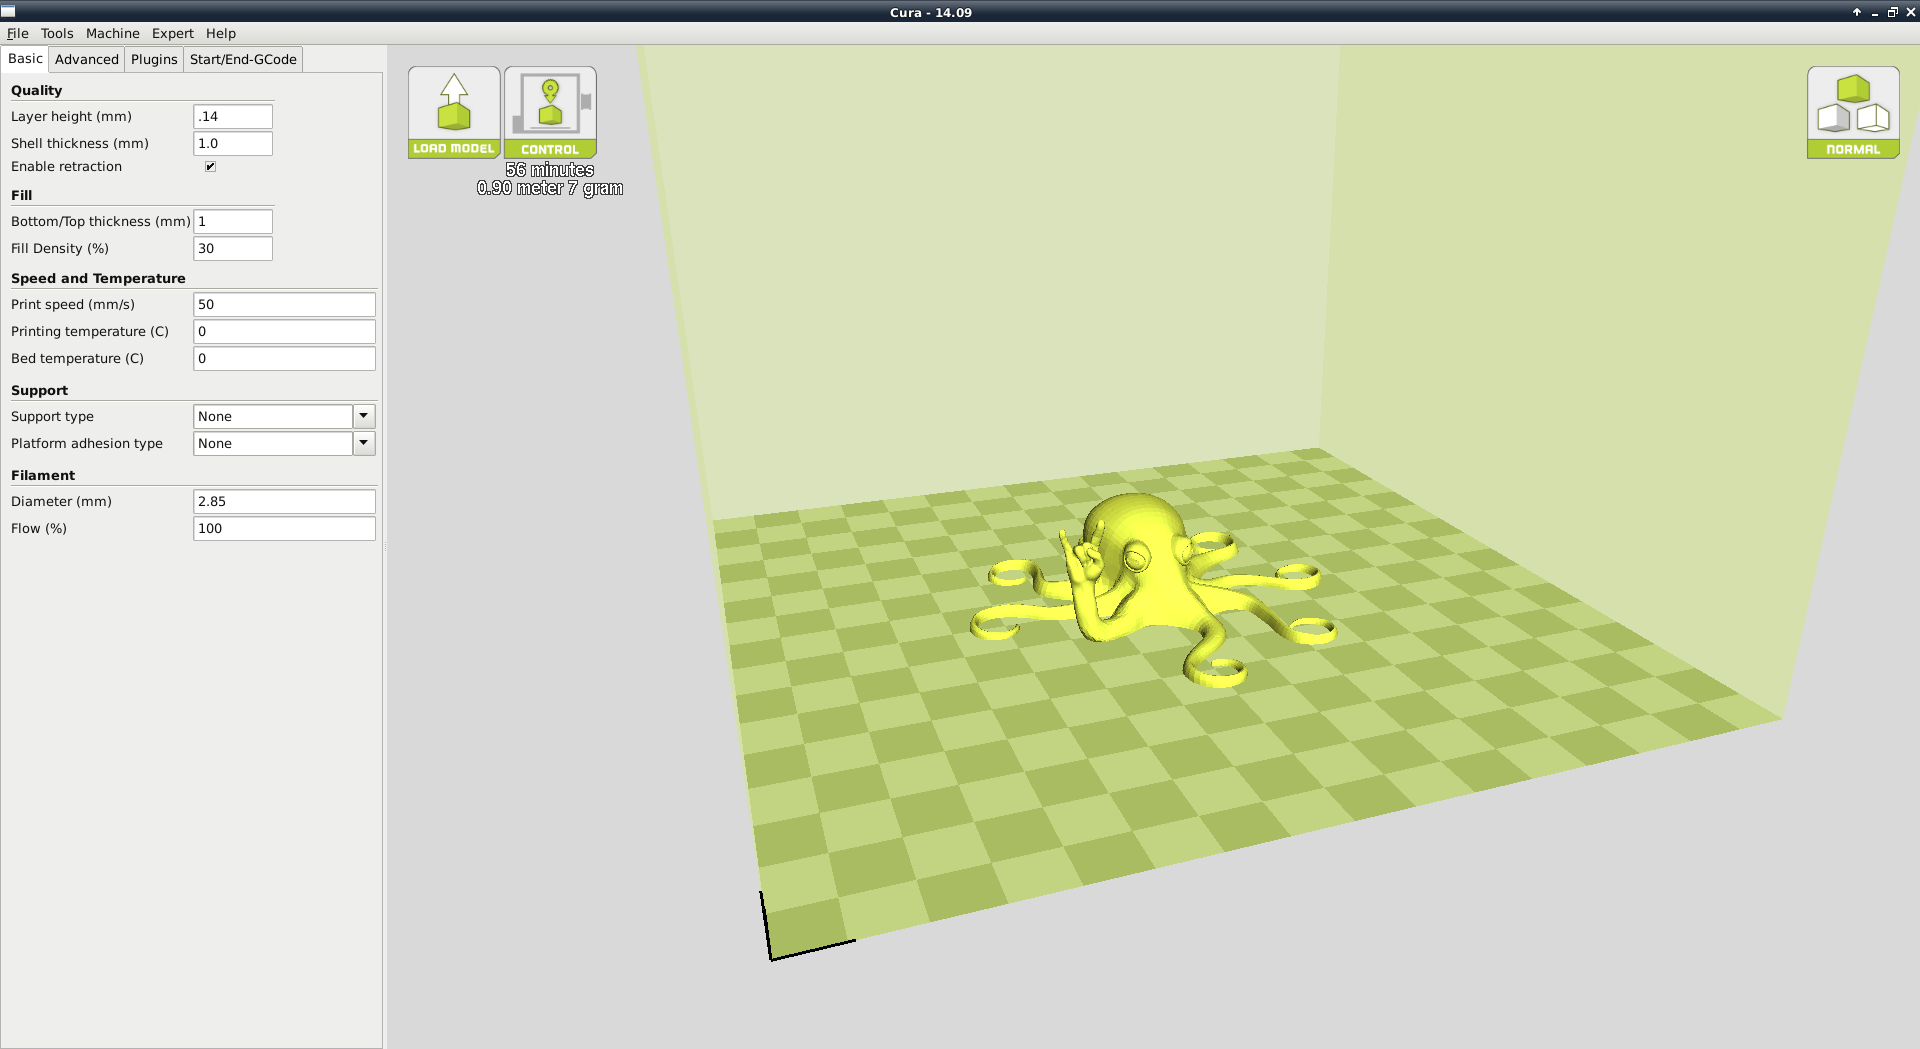
\includegraphics[keepaspectratio=true,angle=0,height=0.4\textheight,width=1.0\textwidth]{Expert.png}
\caption{Full Setting Options}
\label{fig:Expert Options}
\end{figure}

\subsection{View in Full Settings}
\index{Full Settings}
When you first switch to Full Settings, Cura will need to know what filament and quality you wish to use. It will automatically transfer our quickprint settings over to allow adjustments if one is selected. \textcolor{red}{IF A QUICKPRINT PROFILE IS NOT AVAILABLE, YOU WILL NEED TO MANUALLY LOAD ONE IN.} We recommend using our tested profiles that are available here: \texttt{https://www.lulzbot.com/cura}. You will want to choose the profile that matches your filament and quality needs. Once downloaded, you can load the file into Cura by selecting \texttt{File} > \texttt{Open Profile}. Choose your desired profile. This will automatically update all of your settings for use with your printer.
%\begin{figure}[hbt]
%\centering
%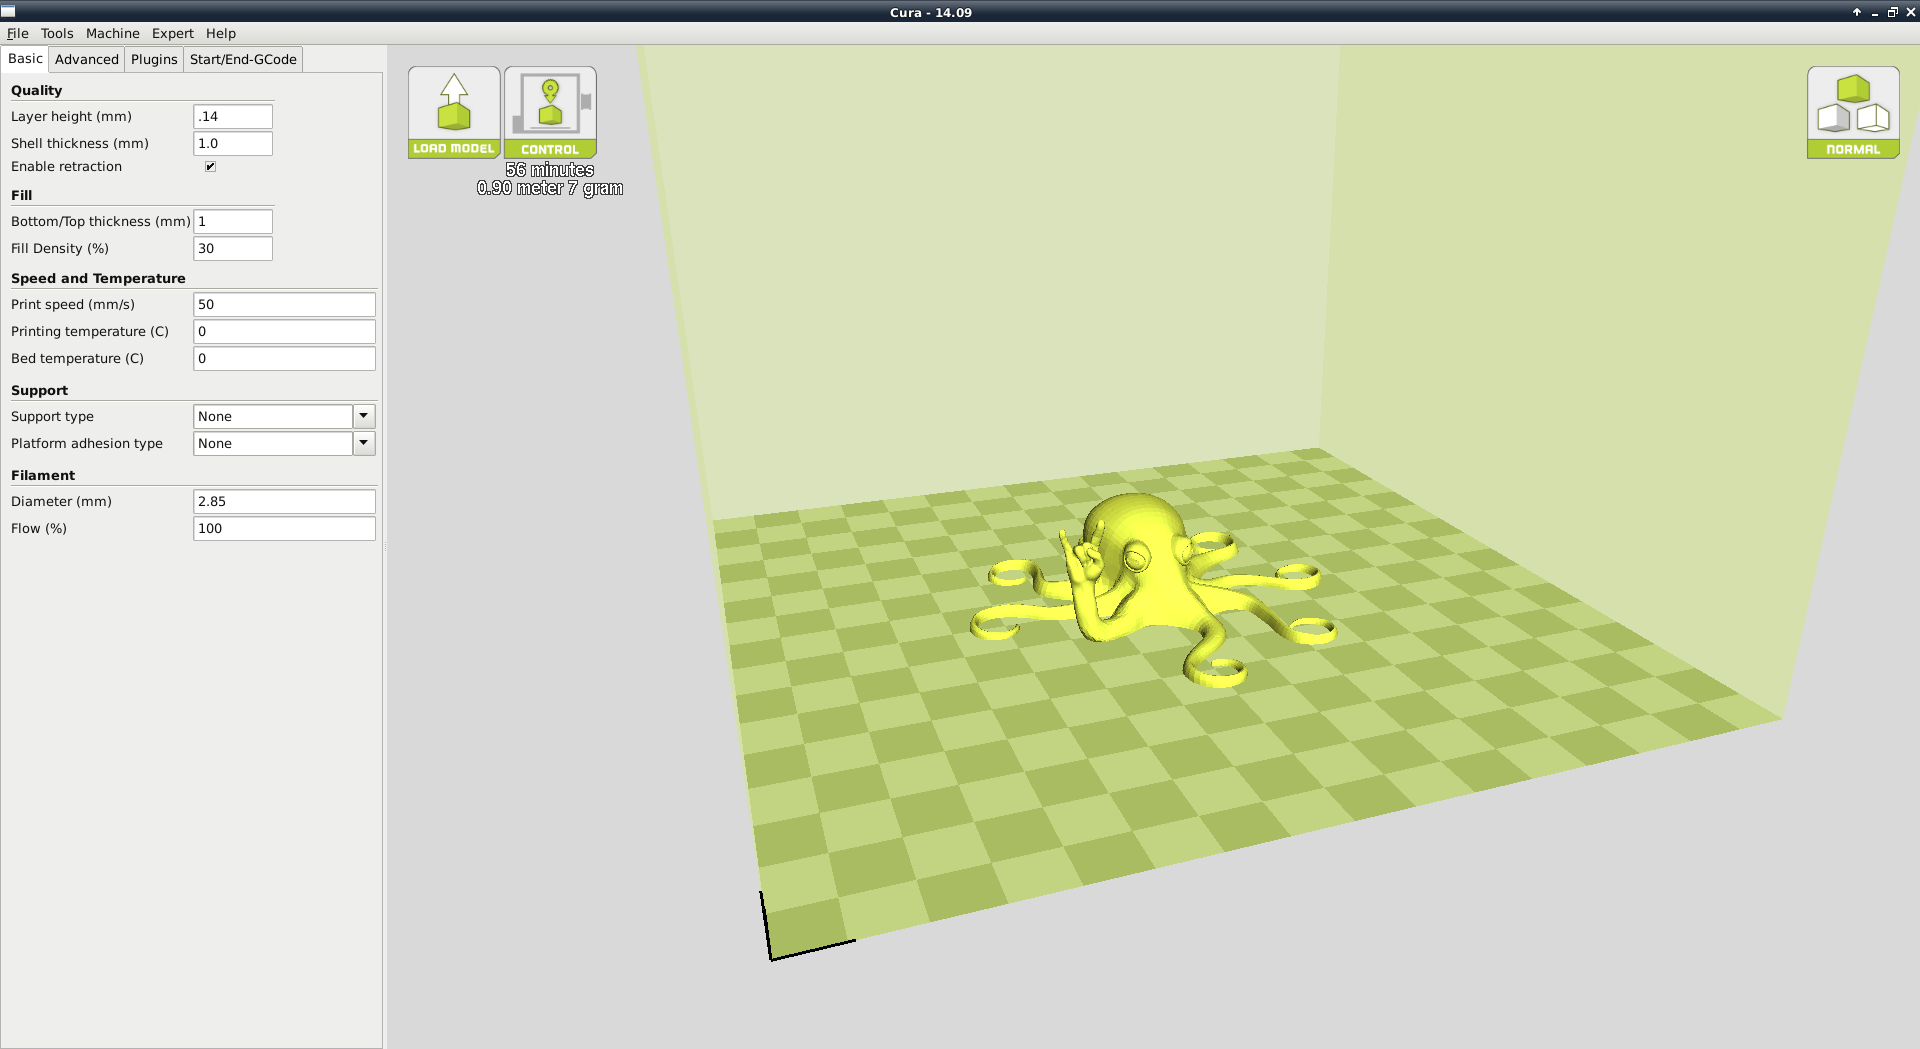
\includegraphics[keepaspectratio=true,angle=0,height=0.4\textheight,width=1.0\textwidth]{Expert.png}
%\caption{View in Full Settings}
%\label{fig:Full Settings View}
%\end{figure}

\section{Basic Tab Options}
\index{Basic Options}

\subsubsection{Layer Height}
\index{Layer Height}
The thickness of each printed layer is known as the ``Layer Height''. The smaller the layer height, the smoother curves will appear. Larger layer heights are better for bridging and overhangs. Smaller layer heights will also increase print time, as it will take more layers to complete the object.
% (Layer height comparison photos)
\begin{figure}[H]
\centering
\includegraphics[keepaspectratio=true,angle=0,height=0.4\textheight,width=1.0\textwidth]{Layer_Height.jpg}
\caption{Differences in Layer Height}
\label{fig:Differences in Layer Height}
\end{figure}


\subsubsection{Shell Thickness}
\index{Shell Thickness}
This defines the number of vertical walls that comprise the outside of your model. We recommend keeping this set to multiples of your nozzle width. Your TAZ 3D printer is equipped with a 0.5mm nozzle. %The TAZ ships with a .5mm nozzle standard, while the Mini has a .5mm nozzle standard.

\subsubsection{Enable Retraction}
\index{Retraction}
Retraction tells your printer to pull filament out of the hot end upon travel moves. Travel moves are when your print head moves from one area of the print, to another without laying down filament. We recommend keeping this on for all filament types, and adjusting the retraction length and speed for the specific filament.
%(Details given in advanced tab section. ((Reference?))

\subsubsection{Bottom/Top Thickness (mm)}
\index{Bottom Thickness}
\index{Top Thickness}
Also known as ``Surface Layers'' this will determine how thick the top and bottom layers are. A larger number here will create a thicker top and bottom which can be helpful for strength, bridging, and quality purposes. We recommend keeping this number as a multiple of your layer height.

\subsubsection{Fill Density}
\index{Fill Density}
This number is expressed as a percentage. 0\% will give a completely hollow print, while 100\% will give you a completely solid object. We have found that 20\% to 40\% fill density is functional for most prints.

\subsubsection{Perimeters Before Infill}
This option will toggle in what order the infill and perimeters are printed. We recommend leaving this toggled.
\subsubsection{Print Speed (mm/s)}
\index{Print Speed}
Your overall printing speed can be adjusted here. If no other speeds are determined in the later sections your printer will automatically default to this speed. This speed will be different, depending on what type of filament you are using.

\subsubsection{Printing Temperature}
\index{Printing Temperature}
%When using different filament materials you'll need to update the desired hot end and heated bed temperature. Any temperatures specified here will be used to automatically set both the hot end and heated bed. Your print will not begin until these temperatures are met. 

%The Mini 3D printer needs to have the temperature specified in order to run through the automatic bed-leveling routine.
%%%% Since the Mini needs to have Gcode temps set in order to run through auto bed leveling, the following statement is only applicable to the TAZ 4 or earlier. %%%%
We recommend leaving this temperature setting to “0”. If you set your temperature in this section your printer will not begin printing until it reaches the EXACT temperature. We recommend setting your printing temperatures through the Printer Interface, or through your LCD.

\subsubsection{Bed Temperature}
\index{Bed Temperature}
We recommend leaving this temperature setting to “0”. If you set your temperature in this section your printer will not begin printing until it reaches the EXACT temperature. We recommend setting your bed temperatures through the Printer Interface, or through your LCD.

\subsection{Support Type}
\index{Support Type}
Some models will require support material in order to print properly. This will usually occur when an object has an angle in relation to the build plate between 0 to 45 degrees. It is highly recommended to orient your object so that it minimizes or eliminates the need for support.

\subsubsection{Touching Buildplate}
This causes the support material to build up between the heated bed and the object. The red example is Touching Buildplate.
% (Photo of Circle inside a square, that is printed vertically. Have samples on photo table. Reference photo below?)

\subsubsection{Everywhere}
This prints support material between the heated bed and object as well as between the object and itself. The green example is Support Everywhere.
% (Photo of Circle inside a square, that is printed vertically, sample on photo table. Reference Photo Below?)
% (Support Comparison Photo)
\begin{figure}[H]
\centering
\includegraphics[keepaspectratio=true,angle=0,height=0.3\textheight,width=1.0\textwidth]{Support_Revised.png}
\caption{Support Types}
\label{fig:Different Types of Support}
\end{figure}

\subsection{Platform Adhesion Type}
\index{Adhesion Type}
Some models have a small surface area contacting the plate. This can create adhesion issues causing your part to pop off at some point during the print. To fix this, use either \texttt{Brim} or \texttt{Raft}. Raft is better used when a model has small heated bed contact points and overhangs.

\subsubsection{Brim}
\index{Brim}
Brim will create a single layer of filament, contacting and surrounding your model. This will increase the surface area of the part contacting the build platform thereby preventing it from popping off the heated bed. Brim will also help in situations where you are seeing corner lift. Brim settings can be adjusted in the \texttt{Expert Settings} options.
% (See Expert Settings/Page REFERENCE)

\subsubsection{Raft}
\index{Raft}
%% Raft is rarely used these days %%
Raft will generate a layer of material underneath your object. Raft was more often used before the addition of heated plates to increase surface area. Raft settings can be adjusted in the \texttt{Expert Settings} options.

\subsection{Filament Diameter}
\index{Filament Diameter}
The filament diameter setting is one of the more important settings. Make sure that you update this value periodically with your average filament diameter. While your filament may be referred to as 3mm, it is more likely going to be near 2.9mm +/- 0.1mm. You will want this to be an accurate average, as it will allow your printer to correctly calculate how much filament it is pulling into the hot end.

\subsection{Filament Flow \%}
\index{Flow Rate}
This controls how much filament your printer is extruding in relation to speed. This setting is mainly used to adjust for filament density variations. Leave this value at 100\% as changing it can lead to surface quality issues.

\section{Advanced Tab Options}
\index{Advanced Options}

\subsection{Nozzle Size (mm)}
\index{Nozzle Size}
%%%% standalone version line %%%%
This defines your nozzle size. The slicing engine uses this value combined with your other settings to determine how quickly to feed filament into your hot end. The TAZ ships with a 0.5mm nozzle. 

%This defines your nozzle size. The slicing engine uses this value combined with your other settings to determine how quickly to feed filament into your hot end. The Mini ships with a 0.5mm nozzle.

\subsection{Retraction Speed (mm/s)}
\index{Retraction Speed}
Retraction Speed determines the speed at which your filament is reversed out of the hot end for travel moves and when changing direction during printing. We recommend keeping this set to 25mm/s or lower.

\subsection{Retraction Distance}
\index{Retraction Distance}
Retraction Distance determines how much filament is pulled out of your hot end on travel moves and when changing direction. You will want to adjust this depending on temperature settings and filament type. Higher thermal retaining filaments such as PLA behave better with a longer retraction distance. We have found anywhere from 1mm to 3mm is a good starting range.
% changed from "1 to 6mm" to remain conservative.

\subsection{Initial Layer Thickness}
\index{Initial Layer}
This will control how thick your first printed layer height is printed onto the heated bed. Having a larger initial layer height will help prevent your part from popping off the plate. All of our standard profiles have a 0.3mm initial layer height. This eliminates the need for adjustments when switching between filaments.  %\textcolor{red}{Your LulzBot\textsuperscript{\miniscule{\texttrademark}} Mini auto leveling system could be affected if you change this from the standard profiles. Adjust at your own risk.}
\subsection{Initial Layer Line Width}
\index{Initial Layer Width}
This will control how wide your first extruded filament path is for the initial layer. A wider line width will help with bed adhesion. We have found 125\% to be a good starting place. For models with moving printed in place parts, a smaller initial layer line width is recommended. %\textcolor{red}{Your LulzBot Mini auto leveling system could be affected if you change this from the standard profiles. Adjust at your own risk.}

\subsection{Cut Off Object Bottom (mm)}
\index{Cut Off Object}
This setting is used to help print models that were not specifically designed for FFF printing. In particular, it is for models that do not have a flat surface to adhere to the plate. It will sink your object Xmm into the build plate, creating a nice flat surface to begin your print. You can also use this option to remove the lower portion of your model, or if carefully measured, cut your part in half for printing object as two halves.
\begin{figure}[H]
\centering
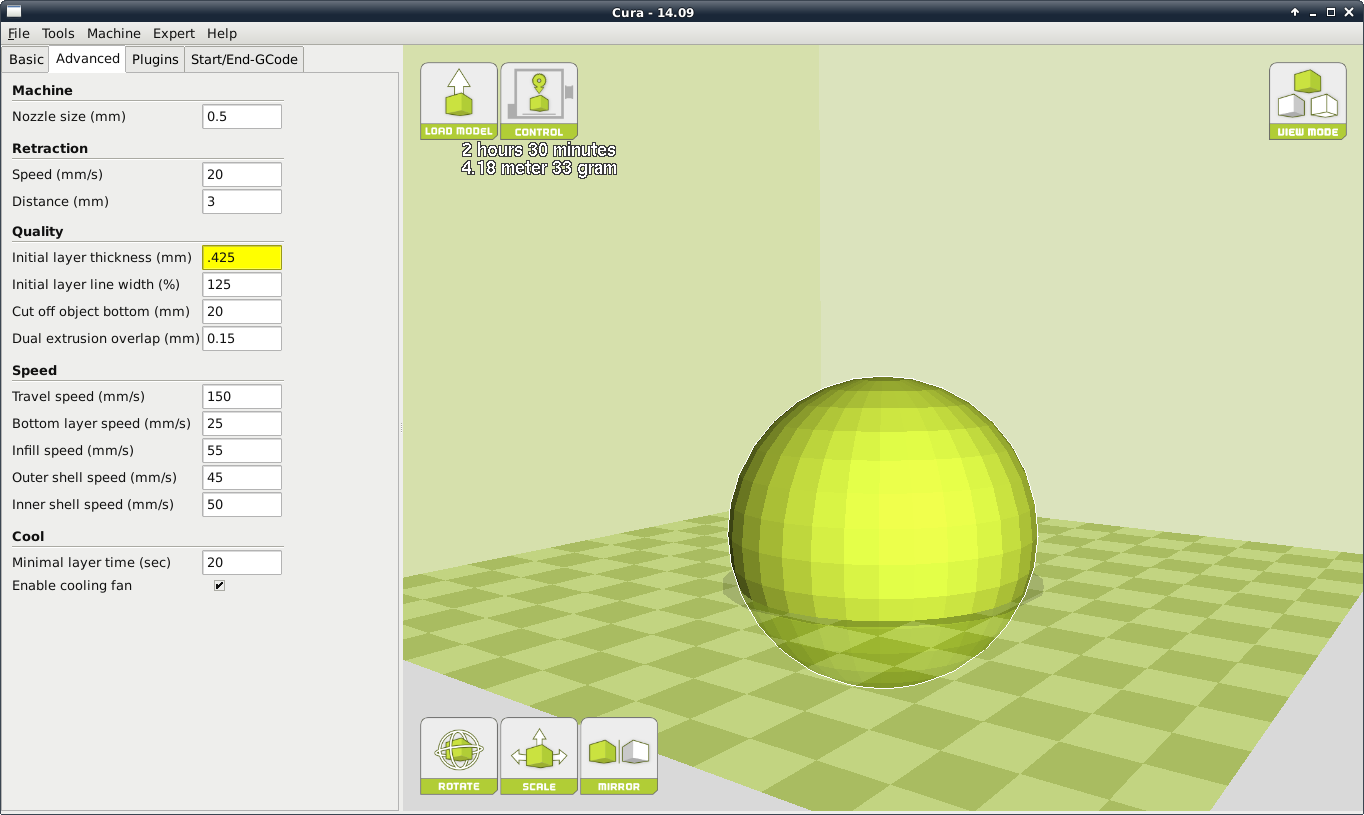
\includegraphics[keepaspectratio=true,angle=0,height=0.4\textheight,width=1.0\textwidth]{cutoff.png}
\caption{Cutoff Example}
\label{fig:Cutoff Example}
\end{figure}

\subsection{Dual Extrusion Overlap}
\index{Dual Extrusion Overlap}
This will determine how far your Dual Extruders will overlap when laying down material. This will help adhesion between the two different colors or types of filament. This setting is only used when the printer is equipped with two hot ends and extruders.

\subsection{Travel Speed}
\index{Travel Speed}
This setting will determine how fast your print head moves while not extruding filament. A normal travel speed of 125 - 175mm/s is recommended.

\subsection{Bottom Layer Speed}
\index{Bottom Layer Speed}
This will control your initial layer speed. In general, a slower initial layer speed will help with first layer adhesion. 

\subsection{Infill Speed}
\index{Infill Speed}
This is how fast your print head speed will be while laying down the interior portion of your model. Faster speeds are usually tolerable here, as none of the infill will be visible from the outside of your object. If you go too fast compared to your inner and outer shells, you can have adhesion issues or globs of filament left behind from the print head.

\subsection{Outer Shell Speed}
\index{Outer Shell Speed}
This will be the outermost surface of the model. This is the most important speed setting, as it controls the speed of your print head on the visible layers. As a general rule of thumb, the slower you go the better looking print you will get. 

\subsection{Inner Shell Speed}
\index{Inner Shell Speed}
This affects vertical walls that are in between the outer shell and infill. This will not be visible but will help support the outer shell and the infill. We recommend keeping this speed setting between your infill and your outer shell speed.

\subsection{Minimal Layer Time}
\index{Minimal Layer Time}
This will determine a minimum amount of time your printer will spend laying down each layer. If your layer print time falls below this your printer will automatically slow down to reach this time before moving onto the next layer. Tweaking this can help get cleaner, crisper prints.

\subsection{Enable Cooling Fan}
\index{Enabling Cooling Fan}
Enables operation of your extruder active cooling fan. The fan settings can be adjusted in the \texttt{Expert Settings} options.

\section{Plugins}
\index{Plugins}
Plugins are custom settings which will alter your print at specific points. The two that come preloaded with Cura are \texttt{Tweak at Z}, and \texttt{Pause at Height}. More plugins and information can be found here: \texttt{http://wiki.ultimaker.com/Category:CuraPlugin} To activate one of these highlight the desired plugin and click the drop-down arrow directly below the Plugins box. 
\begin{figure}[H]
\centering
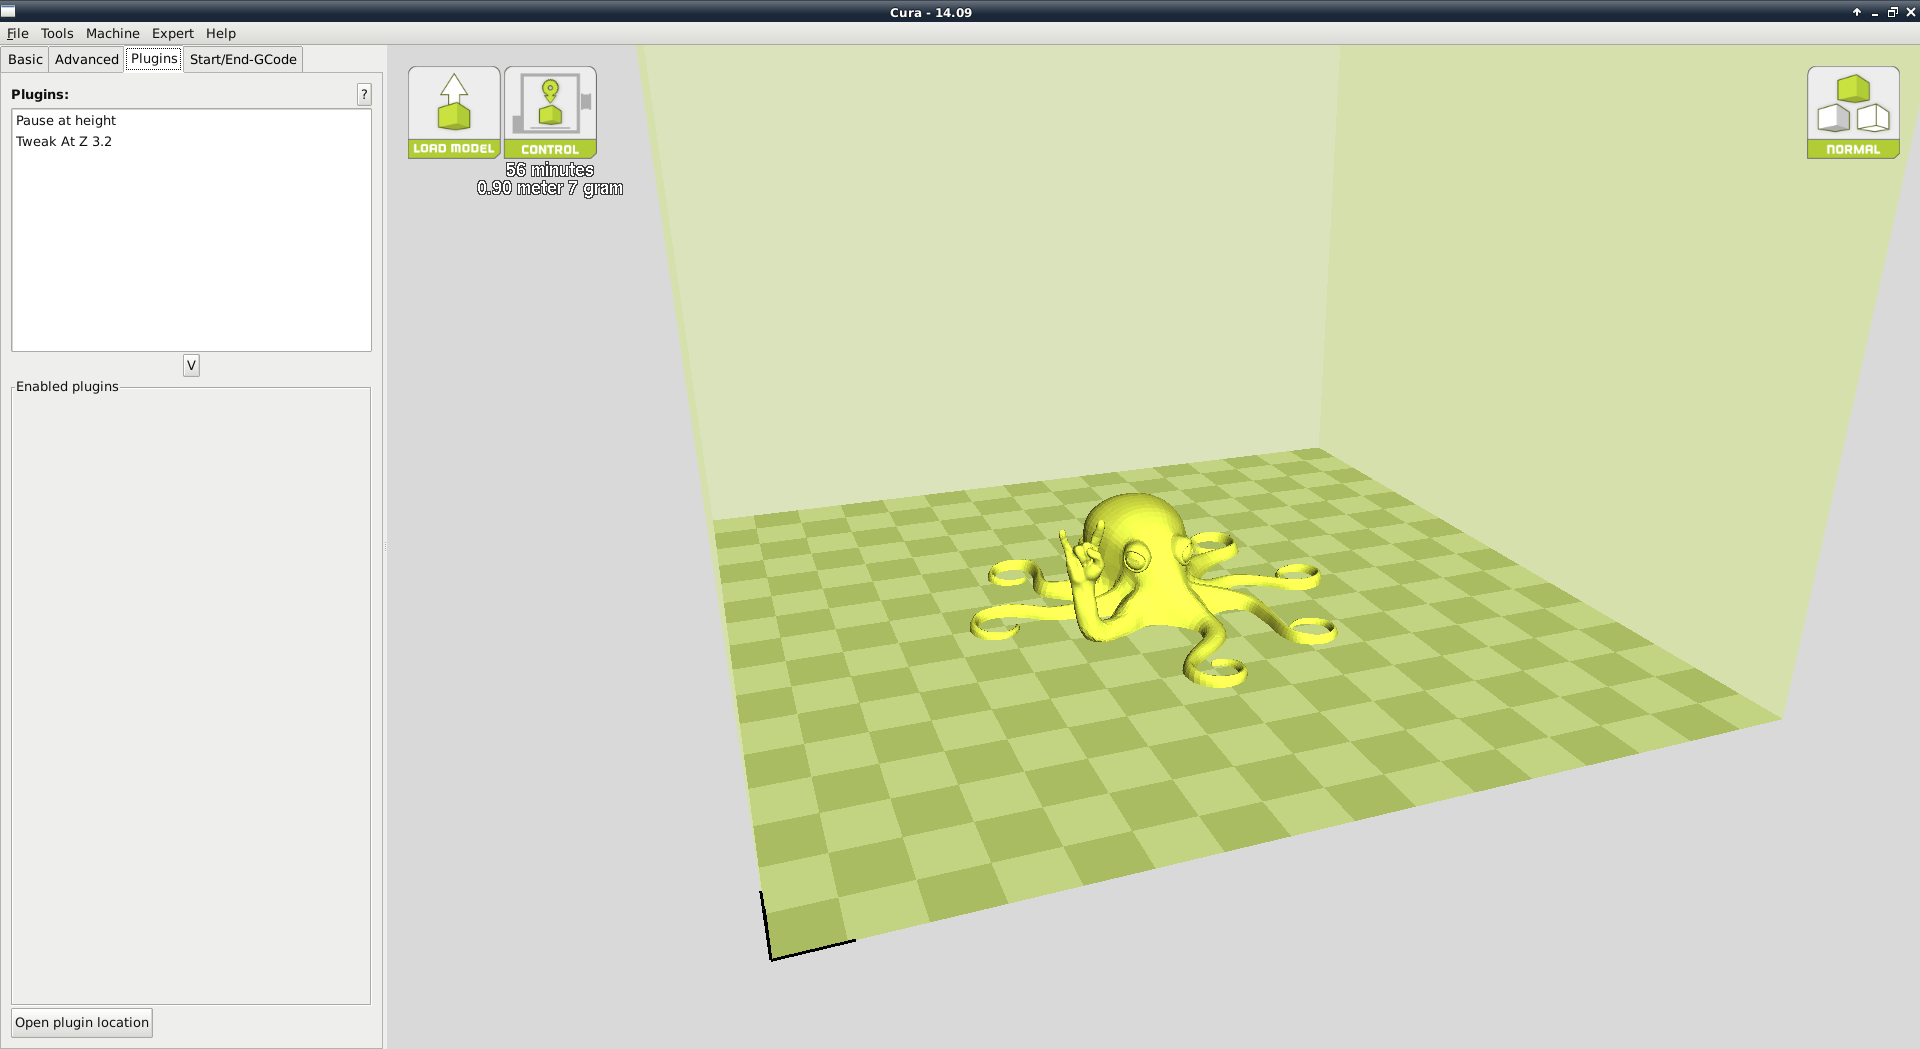
\includegraphics[keepaspectratio=true,angle=0,height=0.4\textheight,width=1.0\textwidth]{Plugins.png}
\caption{View of Plugins}
\label{fig:Plugins}
\end{figure}

\subsection{Tweak at Z}
\index{Tweak at Z}
Make basic changes at specified Z heights. You can determine the Z height or layer count at which you want to make a change. Then choose how you would like to change your settings. You can alter temperatures, fan speeds, and print speeds. Fine tuning these for specific STL files, can produce cleaner prints.

\subsection{Pause at Z Height}
\index{Pause at Z Height}
Pause your print at a specified height. You can also specify where to move the print head and how much filament to retract. This will prevent “blobs” from accumulating on your print while paused. This setting is most commonly used when switching colors of filaments in the middle of a print.

\section{Start and End Gcode Settings}
\index{Custom Gcode}
Custom Gcode allows for complex automatic printer movements and operations. By adding custom Gcode into the start or end of your file, you can alter how it prints. A comprehensive list of Gcode commands can be found here: \texttt{http://reprap.org/wiki/G-code} We recommend new users to leave this as provided in the profiles at \texttt{https://www.lulzbot.com/cura}

%mini
%\subsection{Mini Specific Considerations}
%Please be cautious when changing any of these start and end Gcode settings. \textcolor{red}{This is where your Auto Bed Leveling commands are stored. If improperly altered, your printer will no longer automatically compensate for the heated bed position and can even potentially damage components on the printer.} If you are uncertain of the change you are trying to make, please contact us at \texttt{Support@LulzBot.com} before hand.

\section{Expert Settings}
\index{Expert Settings}
Expert settings will give you more specific options for your retraction, skirt, active cooling, infill, support, brim, raft, and special settings. To gain access to this section you go to \texttt{Expert} > \texttt{Open Full Settings} or on your keyboard press \texttt{Control + E}.
\begin{figure}[H]
\centering
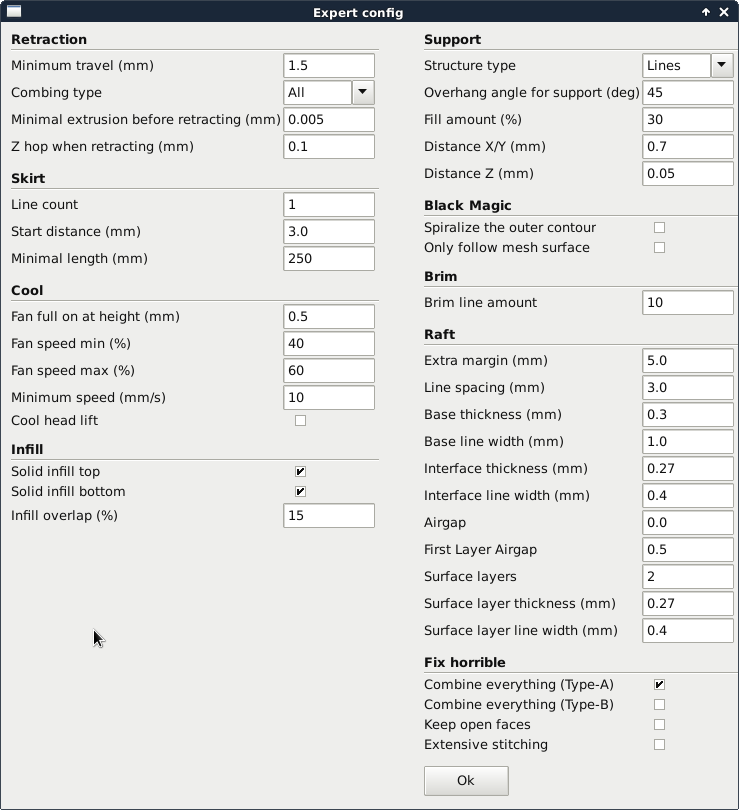
\includegraphics[keepaspectratio=true,angle=0,height=0.4\textheight,width=1.0\textwidth]{Expert_Settings.png}
\caption{View Expert Settings}
\label{fig:Expert Settings}
\end{figure}

\section{Retraction}
\index{Retraction}
Retraction pulls filament out of your nozzle when it is not extruding to prevent your print head from dripping on your object. This section is where you will control how your extruder retracts its filament.

\subsection{Minimum Travel}
\index{Minimum Travel}
This sets the minimum travel distance of your print head in order to retract. If your print head is not moving this far during travel moves, it will not retract.

\subsection{Combing}
\index{Combing}
This option prevents your print head from traveling over holes in the X/Y plane when printing. This will slightly increase print time, but will prevent strings from getting caught on the holes during travel moves. We recommend keeping this setting on.

\subsection{Minimal Extrusion Before Retracting}
This will prevent a retraction move, if your extruder has not put out Xmm of filament since its last retraction.

\subsection{Z Hop When Retracting}
\index{Z hop}
This will raise your print head Xmm while retracting. This setting helps prevent ooze, and strings from being deposited on your print. 
%\textcolor{red}{We do not recommend this setting for TAZ 3 users and earlier. This can cause issues with Z dimensional accuracy.}

\section{Skirt}
\index{Skirt}
Skirt creates a line around the outside of your object. Most commonly used to prime the extruder, in order to prevent missed filament at the beginning of a print. Leave this setting on.

\subsection{Line Count}
\index{Line Count}
This will define the number of loops the Skirt creates around the outside of your object. Smaller models will require more loops to properly prime the extruder.

\subsection{Start Distance}
\index{Start Distance}
This will define the distance away from your model that the skirt will be created. 

\subsection{Minimal Length}
\index{Minimal Length}
This will define the minimum extruded line length for the skirt. This will over ride your line count, producing as many lines as required to reach the minimal length.

\section{Cool}
\index{Cooling}
This section will define how your extruder cooling fan will operate during the print. \textcolor{red}{Your fan will not start until it has reached 25\% or higher for speed settings.} If your print speeds are slowed down due to minimal layer time, the fan will run between minimum and maximum speed based upon how much the layer is slowed down.

\subsection{Fan on at Full Height}
\index{Fan Settings}
This is your Z height where your fan will be turned on to its minimum percentage setting. Especially helpful with high temperature retaining filaments such as PLA. This will be scaled between 0\%, and your minimum fan speed based upon layer height; with it being disabled for the first layer.

\subsection{Fan Speed Min}
\index{Fan Settings}

This will be the speed your fan runs when enabled at full height. Once the Z height is reached for Fan on at Full Height, this will be the speed your fan runs at.

\subsection{Fan Speed Max}
\index{Fan Settings}
This is the fastest speed at which your fan will ever run. When your print speed is slowed down due to minimal layer time, your fan will run between minimum and maximum speed. The maximum fan speed is reached when your printer must be slowed by 50\% or greater.

\section{Support}
\index{Support Material}
You define how your support material is generated here. You must have some form of support turned on in the basic settings in order for these settings to have an effect.

\subsection{Structure Type}
\index{Support Settings}
You can choose between a Grid or a Line pattern for your support material. The grid will be a checkerboard pattern in the X and Y direction. The line option will produce lines in along the y axis for support. The grid will provide stronger support than the line option, but will be harder to remove.

\subsection{Overhang Angle for Support}
\index{Overhang Angle}
This will determine where support material is generated. In general you will be able to print a model with 45 to 90 degree angles in relation to the bed without support. We recommend leaving this setting at 45 degrees.

\subsection{Fill Amount}
\index{Fill Amount}
This will determine how dense your support material is printed, similar to Infill Percentage. The higher percentage, the better support, but it will be harder to remove the support material, will use more material, and will lead to a larger total printing time.

\subsection{Distance X/Y}
\index{Support}
This will determine how far away from your object in the X/Y plane that the support material is being placed.

\subsection{Distance Z}
\index{Support}
This will determine how far away your support material is from your object in the vertical direction. A smaller number here makes for better support, but makes it harder to remove.

\section{Black Magic}
\index{Black Magic}
This section allows you to transform your model into a hollow shell, a single layer thick.

\subsection{Spiralize the Outer Contour}
\index{Spiralize}
This causes your Z axis to be constantly moving upward as printing your single outer wall shell. The results are no layer change lines, giving a much smoother surface. This setting is typically only used for artistic objects as they will be fragile.

\subsection{Only Follow Mesh Surface}
\index{Black Magic}
This will cause your print to follow the outside of your model, building it completely hollow with a single wall outer shell. The only difference between this and Spiralize, is that the Z axis moves regularly. That is, it prints a layer and then moves up to the next one.

\section{Brim}
\index{Brim}
Brim circles the base of the print while making contact, helping adhere the print to the heated plate. This is only one layer thick, and easily removed post-print. This section defines how the brim is formed when brim is activated in basic settings.

\subsection{Brim Line Amount}
This will determine the distance the brim will cover around the outside of your object. The more brim used, the better your part will adhere to the plate. 

\section{Raft}
\index{Raft}
Raft is a platform built underneath your object, designed to help adhesion and prevent warping. It will lay down support material, and then a platform on top of the supports. Your model will be built on top of this platform. The bottom surface of your printed part will not be as clean or as even when using this option. Raft is typically not required.

\subsection{Extra Margin}
\index{Extra Margin}
This determines the distance around the outside of your object that the raft is created. Can be helpful for ensuring no warping of the lower layers.

\subsection{Line Spacing}
\index{Line Spacing}
This will determine the spacing between “support” lines for the raft. A small spacing makes the support structures closer together improving strength of the raft, but uses more material.

\subsection{Base Thickness}
\index{Base Thickness}
This defines how thick your raft will be.

\subsection{Base Line Width}
\index{Base Line Width}
This will define how wide your “support” material is for the raft. This setting will determine how well the surface layers of the raft print.

\subsection{Interface Thickness}
\index{Interface Thickness}
This will determine how thick the surface layers of the raft are. The surface layers are the platform that is built upon the supports.

\subsection{Interface Line Width}
\index{Interface Line Width}
This will determine how wide the top layers of the platform will be. In general, you can keep this set to your nozzle size, as surface quality of the removable raft is not important.

\subsection{Airgap}
\index{Airgap}
This will define the distance between your raft and your print. A larger gap will make your part easier to remove, but will make the bottom of your print look worse.

\subsection{Surface Layers}
\index{Surface Layers}
This will determine the number of layers that create the “platform” of your raft. If you have a wide line spacing, you may want to increase this number to ensure a solid platform. 

\section{Fix Horrible}
\index{Fix Horrible}
These are some of the more advanced and experimental options. They are designed to help repair models with errors to make them suitable for 3D printing. They do not always work. Please be cautious when using these options as they can have unintended effects on your print quality.

\subsection{Combine Everything (Type-A)}
\index{Combine Type-A}
This will attempt to fix all external mesh errors, while keeping internal holes intact. This can accidentally fill in intentional internal holes.

\subsection{Combine Everything (Type-B)}
\index{Combine Type-B}
This will ignore all internal holes of the model and only focus on the external holes. This is helpful when only the outside finish of the model is important.

\subsection{Keep Open Faces}
\index{Open Faces}
This will ignore all manifold errors in the object. It can create issues generating the Gcode as Cura does not know how to interpret the open holes. This option should only be used if you are sure that the holes in the mesh are intended. In general, you should not use this option.

\subsection{Extensive Stitching}
\index{Extensive Stitching}
This causes Cura to automatically add triangle meshes in an attempt to fix manifold errors. This algorithm will greatly increase Gcode generation time and may end up adding in un-intended meshes. It is recommended that you repair your model through MeshLab, FreeCAD or your preferred CAD program before attempting this option.

\section{Dual Extrusion}
\index{Dual Extrusion}
The LulzBot TAZ has the ability to add dual extrusion functionality with the Dual Extruder tool head add-on. We only recommend the Dual Extruder tool head for advanced users. Installation and operation of the dual extruder will require you to flash your firmware, calibrate your extruders, level two heads to a single plane, define extruder offsets, and fine tune your slicing profile. This can be a little overwhelming for new users. We recommended that you have a couple of months of single extruder printing experience before making the switch.

\subsection{Updating Firmware}
\index{Updating Firmware}
In order to use the Dual Extruder you will need to update your firmware to activate the second hot end.

\begin{itemize}
\item Power on your 3D printer and connect it to your computer through USB.
\item Select \texttt{Machine > Machine Settings}.
\item In the top right-hand corner you will see a \texttt{Change Tool Head} button, select this. 
\item Next you will need to select the proper hot end type. Please compare photos with your existing tool head. Choose the correct hot end and select \texttt{Next}.
\item Select the photo that corresponds with your tool head and press \texttt{Next}.
%\item Select the appropriate tool head for your TAZ and select \texttt{Next}.
%\item Choose the correct nozzle size for your machine. If you are not sure what size your printer has use your serial number to determine the nozzle size with the information found at \texttt{https://www.lulzbot.com/printer-identification}.
\item The final step will be \texttt{flashing the firmware}. Choose \texttt{Flash the firmware} to be sure to update the printers firmware to the proper settings. \textcolor{red}{This must be done to allow your printer to operate properly.}
\item Once the progress bar has completed select \texttt{OK > Next > Finish}.  
\item You can verify this by looking at the LCD screen. You should now see three temperature readings. 
\end{itemize} 
You can revert the firmware back to the stock configuration for your LulzBot\textsuperscript{\miniscule{\texttrademark}} 3D printer by selecting \texttt{Machine > Machine Settings > Change Tool Head}. Doing so will overwrite any of your current firmware settings.
%\subsection{Preparing Cura}
%In order to slice for a second tool head, you will need to let Cura know that you have added a second tool head. 
%\begin{itemize} 
%\item Select \texttt{Machine > Machine Settings > Extruder Count > 2}.
%\item Select \texttt{Ok} to close out the screen.
%\item Select \texttt{Machine > Machine Settings} to open the Machine settings again. 
%\item A new section labeled \texttt{Extruder 2} is now present. Within it you will see an \texttt{X offset and Y offset}.
%\item Set the \texttt{X offset to 0} and the \texttt{Y offset to -50}.
%\item Select \texttt{Ok} to save your changes. The Machine settings window will close.
%\end{itemize} 
\subsection{Calibrating Extruders}
\index{Calibrating Extruders}
Each individual extruder will have its own unique set of Esteps. To determine this, you will need to tell the extruder to take in 100mm of filament.
\begin{itemize}
\item Load the outer and inner calibrations squares into Cura \texttt{https://www.lulzbot.com/support/downloads}
\item Open the Printer Interface window and set temperatures for both heads. Switch between hot ends by entering ``\texttt{T0}'' for the rear extruder into the command line terminal. Press \texttt{enter}.
\item Type ``\texttt{T1}'' for the front extruder into the command line terminal. Press \texttt{enter}.
\item Make two marks at 100mm and 120mm on the filament from the top surface of each extruder.
\item Once at the correct extrusion temperature type into the command line ``\texttt{G92}'' and press \texttt{enter}. Then ``\texttt{G1 E100 F60}'' and press \texttt{enter}.
\item Switch to the other tool head by entering ``\texttt{T0}'' for the rear or ``\texttt{T1}'' for the front. 
\item Type into the command line ``\texttt{G92}'' and press \texttt{enter}.
\item Type ``\texttt{G1 E100 F60}'' and press \texttt{enter}.
\item Measure the distance that the tool head over or under extruded. You will need to adjust your Esteps by 8 up or down for each mm it under or over extruded.
\item Update your Esteps for the rear extruder and E1steps for the front extruder through your LCD screen. \texttt{Configuration > Advanced Settings > E/E1 Steps > New Number}. Push in on the knob to exit out of the Esteps entry.
\item Store your new Esteps \texttt{Configuration > Store Memory}.
\end{itemize}

\subsection{Defining Second Extruder Offset}
\index{Second Extruder Offset}
To get crisper looking prints, you will want to really dial in your offsets. With the outer and inner square on your build platform, right click and select \texttt{Dual Extrusion Merge}. The red square will be printed with your front extruder, and the yellow square will be printed with the rear extruder.
\includegraphics[keepaspectratio=true,angle=0,height=0.4\textheight,width=1.0\textwidth]{CalSquares1.png}
After printing the squares, you will want to measure Top, Bottom, Left, and Right gap. Enter these numbers into our offset calculator found here: \texttt{https://www.lulzbot.com/dual-extruder-calibration-calculator} This will produce new offsets, that will need to be updated in the Machine Settings menu. Repeat as many times as desired to truly fine tune the offset. 

\subsection{First Dual Print}
\index{First Dual Print}
When you are ready to produce your first dual extrusion print, you will need to combine the two separate STL files. One STL file will be for each print head. \texttt{Left Click} on whichever STL you would like printed with the \texttt{Rear Tool head}. Then \texttt{Right Click} on whichever STL file you would like printed with the \texttt{Front Tool head} and select dual extrusion merge. You will now see a single model in two colors on the build plate. The red section will be printed with the front extruder, while the green section will be printed with the rear extruder. 
\begin{figure}[H]
\centering
\includegraphics[keepaspectratio=true,angle=0,height=0.4\textheight,width=1.0\textwidth]{PostMerge.png}
\caption{After Merge}
\label{fig:After Merge}
\end{figure}

\begin{figure}
\centering
\includegraphics[keepaspectratio=true,angle=0,height=0.4\textheight,width=1.0\textwidth]{PreMerge.png}
\caption{Before Merge}
\label{fig:Before Merge}
\end{figure}

\subsection{Setting Dual Temps}
\index{Setting Dual Temps}
After your object has been merged as intended, you will need to set the individual temperatures for each print head. In order to switch between which hot end you are heating, you will need to manually enter \texttt{T0} to set temps for the rear hot end, and \texttt{T1} to set temps for the front hot end. \texttt{The Bed temp can be set from either T0 or T1}. Once both print heads and the bed has reached temperature, go ahead and hit \texttt{Print.}

If you have any questions or would like some tips using your dual extruder, reach out to your fellow forum users at \texttt{http://Forum.LulzBot.com}.
}
\fi
%%% END CURA %%%

%%% Pronterface %%%
\ifprintrun
\chapter{\emph{Printrun}}
\thispagestyle{empty}
\markboth{Printrun}{LulzBot TAZ User Manual}
{\include{printrun}}
\fi
%%% END PRONTERFACE %%%

%%% FIRSTPRINT %%%
\iffirstprint
\chapter{\emph{Your First 3D Print}}
\label{firstprint}
\thispagestyle{empty}
\markboth{Your First 3D Print}{LulzBot TAZ User Manual}
{\index{bed leveling}
\section{Bed Leveling}
Make sure you take the time to go through the following procedure to help ensure that your prints are consistent and trouble free. Make sure to first read the instructions for using the Printrun software. Connect to the printer as described in the Printrun software section. Once \texttt{Pronterface} is connected to the printer use the homing buttons to home the X and Y axis. \textcolor{red}{Do not use the \texttt{Home Z button} until after the \texttt{Z axis End stop} has been adjusted. Make sure that the red shipping clamps on the Z axis smooth rods have been removed before continuing.}

\subsection{Rough Adjustment of the Z Axis End Stop Trigger}
\index{end stop}
\begin{figure}[H]
\centering
\includegraphics[keepaspectratio=true,angle=0,height=0.4\textheight,width=1.0\textwidth]{Z_end_stop_trigger.JPG}
\caption{Z end stop trigger}
\label{fig:Z_end_stop_trigger}
\end{figure}
To lower or raise the Z home height adjust the Z end stop trigger. The red end stop trigger is on the far left of the printer mounted on the X-axis motor mount. Before using the \texttt{home Z} button or the \texttt{home all} button you will need to adjust the \texttt{Z axis endstop trigger}. Once connected to the TAZ 3D printer in Pronterface, Rotate the \texttt{Z axis end stop trigger} clockwise to lower the bottom of the screw closer to the Z axis end stop. Once lowered by approximately 1cm, press the \texttt{HomeZ button} to home the Z axis. The hot end will approach the heated bed and should stop around a centimeter above the surface of the heated bed. While the Z axis is moving down pay attention to the Z axis movement and sound. The Z axis stepper motors should be moving in unison. If you notice a grinding sound stop, turn the printer off and before proceeding, make sure that the Z axis looks level in relation to the body of the TAZ 3D printer. Manually rotate one of the Z axis stepper motors by hand if needed to visually level the Z axis.

\index{z axis}
\subsection{Raising the Z Axis}
Use the \texttt{+Z 10 button} to move the Z axis up in \texttt{10mm} increments. \textcolor{red}{Commands sent in Pronterface will stack, so multiple movement button presses can potentially be harmful and cannot be stopped without powering down the 3D printer.} Keep an eye on the nozzle for the hot end. Raise the Z axis until the hot end nozzle is approximately 40-50mm away from the print bed.

\subsection{Verify Z Axis Leveling}
With the Z axis above the bed, use the included \texttt{150mm ruler} to measure the distance from the bottom of the \texttt{X axis} smooth rod and the top surface of the \texttt{Y axis} aluminum bed plate on the left side.
\begin{figure}[H]
\centering
\includegraphics[keepaspectratio=true,angle=0,height=0.4\textheight,width=1.0\textwidth]{X-Y_axes_leveling_check.JPG}
\caption{Verifying the X and Y axis are square}
\label{fig:X-Y_axes_leveling_check}
\end{figure} 
Compare the distance measurement from the left side to the measurement on the right side. The distance measurement should be the same. If not, in Pronterface use the \texttt{Motors off} button to turn off the stepper motors on the TAZ 3D printer. Manually, by hand, turn the threaded rod on one side of the printer to raise or lower that side to match the measurement on the other side. If the Z axis has been adjusted measure again to confirm that the left and right side of the Z axis are level in relation to the Y axis aluminum plate.


\subsection{Fine Adjustment of the Z Axis End Stop}
\begin{comment}
\begin{figure}[H]
\centering
\includegraphics[keepaspectratio=true,angle=0,height=0.4\textheight,width=1.0\textwidth]{Z_end_stop_trigger.JPG}
\caption{Z end stop trigger}
\label{fig:Z_end_stop_trigger}
\end{figure}
\end{comment}
To lower or raise the Z home height adjust the Z end stop trigger. The red end stop trigger is on the far left of the printer mounted on the X-axis motor mount.
Adjust the \texttt{Z axis end stop trigger} by rotating the screw counter-clockwise to raise the tip of the screw. Raise the screw by roughly the same amount of the distance between the nozzle tip and the print surface. Press the \texttt{Home Z} button to home the Z axis. The tip of the nozzle should now be very close to the surface of the bed.

\subsection{Leveling the Print Bed}
Slide a thin piece of paper underneath the nozzle in the front left corner of the bed. Adjust the Z axis end stop and home the Z axis until the tip of the nozzle applies a firm pressure on the paper. Try to slide the paper from underneath the tip of the nozzle. It should not tear, but some resistance should be felt. Move the hot end nozzle tip over to the far side of the X axis by using the \texttt{+X 100 button}. As the X axis carriage approaches the end of the X axis use the \texttt{+X 10 button} and finally the \texttt{+X 1 button}. Once the tip of the nozzle is near the front right corner of the bed slide the same piece of paper under the nozzle and home the Z axis. To raise or lower the front right corner of the bed adjust the third screw from the left. Do not adjust the middle screw. Adjust the front right corner of the bed until the amount of tension felt when moving the piece of paper under the nozzle feels the same as the tension felt when doing the same thing on the front left corner. Repeat the same process using the \texttt{+Y button} to move the heated bed to place the nozzle on the rear right corner of the bed. Adjust the height of the bed using the same procedure as outlined above. Finally, move the X axis carriage over to the rear left corner of the bed and perform the same leveling procedure to adjust the last corner. The bed should now be almost perfectly level. We will check this in a later section. Use the controls in Printrun to raise the Z axis up 20mm, and move the X axis carriage over to the center of the X axis.

\section{Set Temperature}
\index{temperature}
%Make sure to first read the instructions for using the Printrun software. Connect to the printer as described in the Printrun software section
%%% XXX pageref going to \label not \section (page \pageref{Installing Printrun}).
Set the hot end and print surface for ABS or PLA plastic and turn both on. The temperature settings for ABS should be set at \texttt{230°C} for the hot end and \texttt{85°C} for print surface; for PLA they should be set at \texttt{185°C} for the hot end and \texttt{55°C} for print surface. Click the \texttt{Motors Off} button.
\glossary{Idler}{Refers to parts using a bearing (usually a 608ZZ) to add tension in belts or to add pressure against a rolling surface.}
\section{Load Filament}
\index{filament}
\index{hot end}

Once the hot end is heated to the correct temperature you will now need to load the plastic filament into the extruder.
\begin{figure}[hbt]
\centering
\includegraphics[keepaspectratio=true,angle=0,height=0.4\textheight,width=1.0\textwidth]{extruder_idler_release.JPG}
\caption{Extruder idler release}
\label{fig:extruder_idler_release}
\end{figure}
% update feed hole picture.
Gently squeeze both the idler screws and the plastic clip together and pull upwards to release the idler (Fig. \ref{fig:extruder_idler_release}, page \pageref{fig:extruder_idler_release}). The idler screws can be loosened if necessary. The idler can be rotated downwards allowing access to the hobbed bolt and filament feed hole(Fig. \ref{fig:extruder_filament_slot}, page \pageref{fig:extruder_filament_slot}). If the extruder has a small section of filament already loaded, you will need to remove the filament once the extruder idler has been opened, by gently pulling out the filament by hand once the hot end has reached extrusion temperature. From the previously installed filament reel, feed the end of the plastic filament into the filament feed hole
(Fig. \ref{fig:extruder_filament_slot}, page \pageref{fig:extruder_filament_slot}).
\begin{figure}[hbt]
\centering
\includegraphics[keepaspectratio=true,angle=0,height=0.4\textheight,width=1.0\textwidth]{extruder_filament_slot.JPG}
\caption{Extruder filament slot}
\label{fig:extruder_filament_slot}
\end{figure}
Now you can push the filament through the extruder by slowly pushing the filament down into the hot end.

Once the filament extrudes a small amount out of the nozzle raise the idler and slide the two idler bolts and plate back into place. Tighten the two idler bolts if you previously loosened them. Tighten the two screws until they are finger tight, then tighten them slightly more. Now use the \texttt{Extrude} button in Printrun to test that the extruder is working properly. You may need to extrude 40-60mm of filament to fully prime the hot end. Adjust the tension on the two screws until you can reliably and repeatedly extrude roughly 40mm of filament.

\section{Home Printer}
Use the home buttons to home the X axis and then the Y axis. Next home the Z axis. When the Z axis is at home the nozzle tip should be right above the glass
(Fig. \ref{fig:nozzle_height}, page \pageref{fig:nozzle_height}). The image to the left, in figure \ref{fig:nozzle_height}, is the correct nozzle height.
\begin{figure}[p]
\centering
\includegraphics[keepaspectratio=true,angle=0,height=0.4\textheight,width=1.0\textwidth]{nozzle_height.jpg}
\caption{Nozzle height}
\label{fig:nozzle_height}
\end{figure}
\begin{figure}[p]
\centering
\includegraphics[keepaspectratio=true,angle=0,height=0.4\textheight,width=1.0\textwidth]{Z_end_stop_trigger.JPG}
\caption{Z end stop trigger}
\label{fig:Z_end_stop_trigger}
\end{figure}
The nozzle should not be pushing down on the print surface. To lower or raise the Z home height adjust the Z end stop trigger. The red end stop trigger is on the far left of the printer mounted on the X-axis motor mount.
(Fig. \ref{fig:Z_end_stop_trigger}, page \pageref{fig:Z_end_stop_trigger}).
The red end stop trigger can be lowered by turning clockwise and raised by turning counter-clockwise. Once you have homed the axes and the hot end and bed have reached the correct temperature it is time to print!

%fix image positioning, images for 5.3 get shoved underneath 5.4
\section{Z Print Height}
Load the \texttt{bed_level.gcode} file.
This file can be found at: \texttt{http://download.lulzbot.com/TAZ/calibration} . Once downloaded the file your computer, press the \texttt{Load file} button. Navigate through the file browser to the downloaded \texttt{bed\_level.gcode} file, highlight the file and select the \texttt{Open} button.

The .gcode file should appear in the Printrun G-Code viewer. Press the \texttt{Print} button to begin the print. When the print starts make sure the first layer is not printing too close or too far from the print bed. Note 
Figure \ref{fig:1st_layer_adhesion}, page \pageref{fig:1st_layer_adhesion},
\begin{figure}[hbt]
\centering
\includegraphics[keepaspectratio=true,angle=0,height=0.4\textheight,width=1.0\textwidth]{1st_layer_adhesion.jpg}
\caption{First layer adhesion}
\label{fig:1st_layer_adhesion}
\end{figure}
as an example of a good first layer adhesion. From left to right: very low, low, \emph{perfect}, high, very high. If the first layer is too high or low you can pause the print by pressing the \texttt{Pause} button. Adjust the Z end stop trigger. After making adjustments remove any printed material off the bed and home the axes and press \texttt{Restart} to restart the print. Measure the extrusion width, ideally the width would be the same in all areas of the bed. You would raise/lower a corner to minimize/increase the extrusion width to match the others. Once they are all consistent, the bed is level.

\section{Your First Octopus!}
Load the \texttt{octopus.gcode} file. This file can be found at:
\texttt{http://download.lulzbot.com/TAZ/novelties/}. Load the file in Pronterface, bring the hot end \texttt{(230C ABS/185C PLA))} and the heated bed \texttt{(85C ABS/60C PLA)} up to printing temperature. Once the printer is at the appropriate temperature, press the \texttt{Print} button to begin the print.

\section{Remove Part}
After the part is finished printing, the heated bed will automatically cool down to \texttt{60°C}. If you are printing PLA you will need to turn the heated bed off. Once the bed cools you can you pop the finished part off of the printed surface. To remove the printed part, use the clam knife included in your printer kit. Leather gloves are suggested to protect your hands from the clam knife blade. It is also safe practice to not place your hand behind the direction you are pushing the clam knife. Using the side of the clam knife blade pry up one side of the printed part. If your part is large you may need to pry at multiple points to pop the part off of the print surface. When removing parts take caution to not damage the PET film. If the film is cut or ripped it will peel from the glass and need to be replaced. Make sure to reset the heated bed to the correct temperature and allow it to heat up to the needed temperature before starting the next print.

}
\fi
%%% END FIRSTPRINT %%%

%%% SLIC3R %%%
\ifslicer
\chapter{\emph{Slic3r}}
\thispagestyle{empty}
\markboth{Slic3r}{LulzBot TAZ User Manual}
{%
% Slicer.tex
% Slic3r ....
%
% LulzBot™ TAZ User Manual
%
% Copyright (C) 2015 Aleph Objects, Inc.
%
% This document is licensed under the Creative Commons Attribution 4.0
% International Public License (CC BY-SA 4.0) by Aleph Objects, Inc.
%

\section{\texttt{Introduction}}
%!TEX root = Slic3r-Manual.tex
\subsection{Overview}
Slic3r is a tool which translates digital 3D models into instructions that are understood by a 3D printer.  It slices the model into horizontal layers and generates suitable paths to fill them.

Slic3r is already bundled with the many of the most well-known host software packages: Pronterface, Repetier-Host, ReplicatorG, and can be used as a standalone program.

This manual will provide guidance on how to install, configure and utilise Slic3r in order to produce excellent prints.


\subsection{Goals \& Philosophy}
Slic3r is an original project started in 2011 by Alessandro Ranellucci (aka. Sound), who used his considerable knowledge of the Perl language to create a fast and easy to use application.  Readability and maintainability of the code are among the design goals.

The program is under constant refinement, from Alessandro and the other contributors to the project, with new features and bug fixes being released on a regular basis.


\subsection{Donating}
Slic3r started as a one-man job, developed solely by Alessandro in his spare time, and as a freelance developer this has a direct cost for him.  By generously releasing Slic3r to the public as open source software, under the GPL license, he has enabled many to benefit from his work.

The opportunity to say thank you via a donation exists.  More details can be found at: \texttt{http://slic3r.org/donations}.


\section{\texttt{Getting Slic3r}}
%!TEX root = Slic3r-Manual.tex
\index{download}
\index{binaries}
\index{Source Code}
\index{GitHub}
\index{license}

\fbox{
	\parbox{\linewidth}{
		Slic3r is Free Software, and is licensed under the GNU Affero General Public License, version 3.
	}
}	

\subsection{Downloading}

\subsubsection{From LulzBot.com} % (fold)
\label{sub:from_LulzBot}
The Slic3r version that has been tested for the TAZ printer can be downloaded from the LulzBot.com downloads page: \texttt{https://www.lulzbot.com/Slic3r}.

Pre-compiled packages are available for Windows, Mac OS X and Linux.  Windows and Linux users can choose between 32 and 64 bit versions to match their system.
% subsubsection From LulzBot (end)

\subsubsection{Slic3r} % (fold)
\label{sub:slic3r}
Slic3r can be downloaded directly from: \texttt{http://slic3r.org/download}.

Pre-compiled packages are available for Windows, Mac OS X and Linux.  Windows and Linux users can choose between 32 and 64 bit versions to match their system.
% subsubsection slic3r (end)

\subsubsection{Manual} % (fold)
\label{sub:manual}

The latest version of full Slic3r manual, with {\LaTeX} source code, can be found at: \texttt{https://github.com/alexrj/Slic3r-Manual}

% subsubsection manual (end)

\subsubsection{Source} % (fold)
\label{sub:source}

The source code is available via GitHub: \texttt{https://github.com/alexrj/Slic3r}. For more details on building from source see §\ref{sec:building_from_source} below.

% subsubsection source (end)

\subsection{Installing}

\subsubsection{Linux}

Extract the archive to a folder of your choosing.
Either:
\begin{itemize}
\item Start Slic3r directly by running the Slic3r executable, found in the bin directory, or
\item Install Slic3r by running the do-install executable, also found in the bin folder.
\end{itemize}
The archive file may then be deleted.

\subsubsection{Windows}

Unzip the downloaded zip file to a folder of your choosing, there is no installer script. The resulting folder contains two executables:
\begin{itemize}
\item \texttt{slic3r.exe} - starts the GUI version.
\item \texttt{slic3r-console.exe} - can be used from the command line.
\end{itemize}

The zip file may then be deleted.

\subsubsection{Mac OS X}

Double-click the downloaded dmg file, an instance of Finder should open together with an icon of the Slic3r program.  Navigate to the Applications directory and drag and drop the Slic3r icon into it.
The dmg file may then be deleted.



\subsection{Building from source} % (fold)
\label{sec:building_from_source}

For those wishing to live on the cutting edge, Slic3r can be compiled from the latest source files found on GitHub \texttt{https://github.com/alexrj/Slic3r}.

Up-to-date instructions for compiling and running from source can be found on the Slic3r wiki.

%\begin{itemize}
%   \item \textbf{GNU Linux} \par \texttt{https://github.com/alexrj/Slic3r/wiki/Running-Slic3r-from-git-on-GNU-Linux}
%    \item \textbf{OS X} \par	\texttt{https://github.com/alexrj/Slic3r/wiki/Running-Slic3r-from-git-on-OS-X}
%    \item \textbf{Windows} \par	\texttt{https://github.com/alexrj/Slic3r/wiki/Running-Slic3r-from-git-on-Windows}

%\end{itemize}


\section{\texttt{First Print}}
%!TEX root = Slic3r-Manual.tex

%!TEX root = Slic3r-Manual.tex
\begin{comment}
\index{calibration}
\subsection{Calibration}
\label{calibration}
Before even attempting the first print it is vital that the printer is correctly calibrated.  Skipping or rushing this step will result in frustration and failed prints later, so it is important to take the time to make sure the machine is correctly set up.

Each machine may have it's own calibration procedure and this manual will not attempt to cover all the variations.  Instead here is a list of key points that should be addressed. 

\begin{itemize}
\item Frame is stable and correctly aligned.
\item Belts are taut.
\item Bed is level in relation to the path of the extruder.
\item Filament rolls freely from the spool, without causing too much tension on the extruder.
%\item Current for stepper motors is set to the correct level.
\item Firmware settings are correct including: axis movement speeds and acceleration; temperature control; end-stops; motor directions.
\item Extruder is calibrated in the firmware with the correct steps per mm of filament.
\end{itemize}

The point regarding the extruder step rate is vital.  Slic3r expects that the machine will accurately produce a set amount of filament when told to do so.  Too much will result in blobs and other imperfections in the print.  Too little will result in gaps and poor inter-layer adhesion.

Please refer to the printer documentation and/or resources in the 3D printing community for details on how best to calibrate a particular machine.
/begin{comment}


\newpage

%!TEX root = Slic3r-Manual.tex

\subsection{\texttt{Configuration Wizard}}
\label{sec:configuration_wizard}
\index{Configuration Wizard}

Slic3r has two features to aid newcomers: the configuration wizard, and simple mode.

Sometimes it is nice to have a helping hand when starting out with new software.  The configuration wizard asks a series of questions and creates a new configuration for Slic3r.

\textbf{When using the pre-set TAZ Slic3r profiles you do not need to complete the Configuration Wizard.} The Configuration Wizard can be later accessed from the top menu once you are ready to start creating your own Slic3r profiles.

\begin{figure}[H]
\centering
\includegraphics[keepaspectratio=true,width=\textwidth]{configuration_wizard/configuration_wizard_welcome.png}
\caption{Configuration Wizard: Welcome Screen}
\label{fig:configuration_wizard_welcome_screen}
\end{figure}

\newpage
\subsubsection{\texttt{1. Firmware Type}}
\label{sub:1_firmware_type}
\index{Printer Settings!Firmware!G-code flavour}
The gcode produced by Slic3r is tailored to particular types of firmware.  The first step prompts for the firmware that the printer uses.  For the TAZ printer select \texttt{RepRap (Marlin/Sprinter)}
\begin{figure}[H]
\centering
\includegraphics[keepaspectratio=true,width=\textwidth]{configuration_wizard/configuration_wizard_firmware_type.png}
\caption{Configuration Wizard: Firmware Type}
\label{fig:configuration_wizard_firmware_type}
\end{figure}

\newpage
\subsubsection{\texttt{2. Bed Size}}
\label{sub:2_bed_size}
\index{Printer Settings!Size and coordinates!Bed size}
This setting defines the maximum distance the extruder may travel along the X and Y axis.  The dimensions for the TAZ print surface are X: 298 and Y: 275.

Be sure to measure from the lower left corner where the extruder nozzle rests when are the home position to the maximum distance the nozzle can travel in each direction.  Take into account that the X carriage may touch the frame before the nozzle reaches it's full distance, this will depend on the printer make and model.

\begin{figure}[H]
\centering
\includegraphics[keepaspectratio=true,width=\textwidth]{configuration_wizard/configuration_wizard_bed_size.png}
\caption{Configuration Wizard: Bed Size}
\label{fig:configuration_wizard_bed_size}
\end{figure}

\newpage
\subsubsection{\texttt{3. Nozzle Diameter}}
\label{sub:3_nozzle_diameter}
\index{Printer Settings!Extruder!Nozzle diameter}
The diameter of the hot-end nozzle is usually clearly displayed either in the description of the hot-end, or in the associated documentation, when the hot-end is purchased.  The nozzle sizes available for the TAZ hot end are 0.35mm and 0.50mm.

If the nozzle was home-made, or came from a source without a diameter given, then carefully measure the aperture as accurately as possible.  One way of determining nozzle size is to very slowly (1mm/s) extrude some filament into free air and measure the thickness of the resulting extrusion\footnote{\	http://forums.reprap.org/read.php?1,113374,113953}.  This has the benefit of taking die swell into account, and consequently may be a useful thing to do even if the diameter is known.

\begin{figure}[H]
\centering
\includegraphics[keepaspectratio=true,width=\textwidth]{configuration_wizard/configuration_wizard_nozzle_diameter.png}
\caption{Configuration Wizard: Nozzle Diameter}
\label{fig:configuration_wizard_nozzle_diameter}
\end{figure}

\newpage
\subsubsection{\texttt{4. Filament Diameter}}
\label{sub:4_filament_diameter}
\index{Filament Settings!Filament!Diameter}
For Slic3r to produce accurate results it must know as accurately as possible how much material is pushed through the extruder.  Therefore it is vital to give it as precise a value as possible for the filament diameter.

Although the filament used in FDM printers is sold as being either 3mm or 1.75mm this is only a general guide.  The diameter can vary between manufacturers and even between batches.  Therefore it is highly recommended to take multiple measurements from along a length of the filament and use the average.  For example, measurements of 2.89, 2.88, 2.90 and 2.91 would yield an average of 2.895, and so this would be used.

\begin{figure}[H]
\centering
\includegraphics[keepaspectratio=true,width=\textwidth]{configuration_wizard/configuration_wizard_filament_diameter.png}
\caption{Configuration Wizard: Filament Diameter}
\label{fig:configuration_wizard_filament_diameter}
\end{figure}

\newpage
\subsubsection{\texttt{5. Extrusion Temperature}}
\label{sub:5_extrusion_temperature}
\index{Filament Settings!Temperature!Extruder}
The extrusion temperature will depend on the material, and most can operate over a range of temperatures.  The supplier should provide guidance as to which temperatures are suitable.  A very general rule of thumb is that PLA lies between 160°C and 230°C, and ABS lies between 220°C and 240°C. More exotic materials will have a different range.

This is one parameter which you will want to fine tune when you start producing prints.  The optimal temperature can vary even between colors of the same material.  Another factor which may affect the chosen temperature is how fast the extrusion is, where generally faster extrusion runs hotter.

\textbf{Note: One may choose to control the extruder temperature manually from the printer controller. In this case the temperature can be set to zero.}

\begin{figure}[H]
\centering
\includegraphics[keepaspectratio=true,width=\textwidth]{configuration_wizard/configuration_wizard_extrusion_temperature.png}
\caption{Configuration Wizard: Extrusion Temperature}
\label{fig:configuration_wizard_extrusion_temperature}
\end{figure}

\newpage
\subsubsection{\texttt{6. Bed Temperature}}
\label{sub:6_bed_temperature}
\index{Filament Settings!Temperature!Bed}
If the printer has a heated bed then this parameter may be set.  As with the extruder temperature, the value will depend on the material used.  A rule of thumb is that PLA requires 35°C - 60°C and ABS requires 85°C.

\textbf{Note: One may choose to control the bed temperature manually from the printer controller. In this case the temperature can be set to zero.}

\begin{figure}[H]
\centering
\includegraphics[keepaspectratio=true,width=\textwidth]{configuration_wizard/configuration_wizard_bed_temperature.png}
\caption{Configuration Wizard: Bed Temperature}
\label{fig:configuration_wizard_bed_temperature}
\end{figure}

\newpage

At this stage the wizard is complete and the basic configuration is defined.

\begin{figure}[H]
\centering
\includegraphics[keepaspectratio=true,width=\textwidth]{configuration_wizard/configuration_wizard_end.png}
\caption{Configuration Wizard: End}
\label{fig:configuration_wizard_end}
\end{figure}



\newpage

%!TEX root = Slic3r-Manual.tex

\subsection{The Important First Layer}
\label{sec:the_important_first_layer}
\index{First Layer}
Before delving into producing the first print it is worthwhile taking a little detour to talk about the importance of getting the first layer right.  As many have found through trial and error, if the first layer is not the best it can be then it can lead to complete failure, parts detaching, and warping.  There are several techniques and recommendations one can heed in order to minimise the chance of this happening.

\paragraph{Level bed.} % (fold)
\label{par:level_bed}
Having a level bed is critical.  If the distance between the nozzle tip and the bed deviates by even a small amount it can result in either the material not lying down on the bed (because the nozzle is too close and scrapes the bed instead), or the material lying too high from the bed and not adhering correctly.
% paragraph level_bed (end)

\paragraph{Higher temperature.} % (fold)
\label{par:higher_temperature}
The extruder hot-end and bed, if it is heated, can be made hotter for the first layer, thus decreasing the viscosity of the material being printed.  As a rule of thumb, an additonal 5° is recommended.
% paragraph higher_temperature (end)

\paragraph{Lower speeds.} % (fold)
\label{par:lower_speeds}
Slowing down the extruder for the first layer reduces the forces applied to the molten material as it emerges, reducing the chances of it being stretched too much and not adhering correctly.  30\% or 50\% of the normal speed is recommended.
% paragraph lower_speeds (end)

\paragraph{Correctly calibrated extrusion rates.} % (fold)
\label{par:correct_extrusion_settings}
If too much material is laid down then the nozzle may drag through it on the second pass, causing it to lift off the bed (particularly if the material has cooled).  Too little material may result in the first layer coming loose later in the print, leading either to detached objects or warping.  For these reasons it is important to have a well-calibrated extrusion rate as recommended in §\ref{calibration}).
% paragraph correct_extrusion_settings (end)

\paragraph{First layer height.} % (fold)
\label{par:first_layer_height}
A thicker layer height will provide more flow, and consequently more heat, making the extrusion adhere to the bed more.  It also gives the benefit of giving more tolerance for the levelness of the bed.  It is recommended to raise the first layer height to match the diameter of the nozzle, e.g. a first layer height of 0.35mm for a 0.35mm nozzle.
Note: The first layer height is set this way automatically in simple mode.
% paragraph first_layer_height (end)

\paragraph{Fatter extrusion width.} % (fold)
\label{par:wider_extrusion_width}
The more material touching the bed, the better the object will adhere to it, and this can be achieved by increasing the extrusion width of the first layer, either by a percentage or a fixed amount.  Any spaces between the extrusions are adjusted accordingly.

A value of approximately 200\% is usually recommended, but note that the value is calculated from the layer height and so the value should only be set if the layer height is the highest possible.  For example, if the layer height is 0.1mm, and the extrusion width is set to 200\%, then the actual extruded width will only be 0.2mm, which is smaller than the nozzle.   This would cause poor flow and lead to a failed print.  It is therefore highly recommended to combine the high first layer height technique recommended above with this one. Setting the first layer height to 0.35mm and the first extrusion width to 200\% would result in a nice fat extrusion 0.65mm wide.
% paragraph wider_extrusion_width (end)

\paragraph{Bed material.} % (fold)
\label{par:bed_material}
Many options exist for the material to use for the bed, and preparing the right surface can vastly improve first layer adhesion.

PLA is more forgiving and works well on PEI, PET, Kapton, or blue painters tape.

ABS usually needs more cajoling. While it's generally preferred to print directly on the PEI surface, a watered-down PVA or white school-glue solution can help prints adhere to the bed and is preferred. \textcolor{red}{Never use anything with acetone on the PEI print surface as it can degrade the PEI material}. 
% paragraph bed_material (end)

\paragraph{No cooling.} % (fold)
\label{par:no_cooling}
Directly related with the above, it makes no sense to increase the temperature of the first layer and still have a fan or other cooling mechanism at work.  Keeping the fan turned off for the first few layers is generally recommended.
% paragraph no_cooling (end)


\newpage

%!TEX root = Slic3r-Manual.tex
\subsection{Working with Models}
\label{sub:working_with_models}
\index{models}

Yet another step lies between now and the first print - a model has to found and then sliced.

\subsubsection{Model Formats} % (fold)
\label{sub:model_formats}
\index{STL}
\index{AMF}
\index{OBJ}

Slic3r accepts the following file types.

\begin{itemize}
	\item STereoLithography (STL) files can come from a wide variety of sources and are now a de facto standard in 3D printing.  The files simply describe the surface geometry of a 3D object without any additional information (such as color or material), and it is this simplicity that has probably made the format ubiquitous.
	\item Wavefront OBJ files are an open format originally used in an animation application from Wavefront Technologies, but has since been adopted by the wider 3D modelling community.  It is similar to the STL format.
	\item Additive Manufacturing File Format (AMF) was developed in response to the limited nature of the STL format.  In addition to describing the geometry of the 3D model it can also describe colors and materials, as well as more complex attributes, such as gradient mixes and multiple object arrangements (constellations).  Whilst the format is deemed a standard it has yet to be widely adopted in the 3D maker community.
\end{itemize}
% subsubsection model_formats (end)

\subsubsection{Finding Models} % (fold)
\label{sub:finding_models}
\index{models!finding}

The 3D model files may come from an online repository, such as Thingiverse\footnote{http://www.thingiverse.com} or GrabCAD\footnote{http://grabcad.com}, or be created from a CAD program, such as FreeCAD\footnote{http://sourceforge.net/projects/free-cad}, Sketchup\footnote{http://www.sketchup.com}, or OpenSCAD\footnote{http://www.openscad.org}, or an online CAD tool such as Shapesmith\footnote{http://shapesmith.net}.

You may wish to view the files before slicing and there are many free applications available, one of which is Meshlab\footnote{http://www.meshlab.org} - a comprehensive tool for viewing and working with 3D files.

\begin{figure}[H]
\centering
\includegraphics[keepaspectratio=true,width=0.75\textwidth]{working_with_models/shapesmith.png}
\caption{Shapesmith online CAD tool.}
\label{fig:shapesmith}
\end{figure}

% subsubsection working_with_models (end)


\subsubsection{Working with Plater} % (fold)
\label{sub:working_with_plater}
\index{Plater}
Slic3r has a tool, called Plater, which allows one or more models to be loaded and arranged before being sliced.

\begin{figure}[H]
\centering
\includegraphics[keepaspectratio=true,width=1\textwidth]{working_with_models/plater.png}
\caption{Plater}
\label{fig:plater}
\end{figure}

Once you have acquired a model, drag it onto the Plater window (or use the Add button below the file list) to load it into Slic3r.  In the figure below, the traditional RepRap Minimug\footnote{http://www.thingiverse.com/thing:18357} is loaded, and is viewed from above. The ring around the model is a skirt - a single perimeter, several millimeters away from the model, which is extruded first.  This is useful in making sure the plastic is flowing smoothly from the nozzle when the model is starting to be printed.

\begin{figure}[H]
\centering
\includegraphics[keepaspectratio=true,width=0.75\textwidth]{working_with_models/minimug_model.png}
\caption{Minimug model.}
\label{fig:minimug_model}
\end{figure}

\begin{figure}[H]
\centering
\includegraphics[keepaspectratio=true,width=1\textwidth]{working_with_models/plater_model_loaded.png}
\caption{STL file loaded.}
\label{fig:plater_model_loaded}
\end{figure}

The model can be repositioned by dragging the representation of it on the left of the screen around the bed.  Note that the dimensions of the bed should match your printer, as given during the initial configuration above.

On the right-hand side is the list of currently loaded files.  The buttons along the top of the file list allow you to arrange the models.
\begin{itemize}
	\item \textbf{More/Less}  - Adjust how many copies should be printed.
	\item \textbf{45°/Rotate}  - Rotate the selected model around the Z axis, either in 45° increments clockwise or counter-clockwise, or by a given amount.
	\item \textbf{Scale}  - Increase or decrease the size of the printed model.
	\item \textbf{Split}  - Divides a model which consists of more than one part into it's constituent parts, allowing each one to be arranged individually.
\end{itemize}

The buttons along the bottom of the file list allow you to add, remove, auto-arrange, or export the models.
\begin{itemize}
	\item \textbf{Add}  - Opens a file dialog to add a model to the plater, as an alternative to dropping a file directly.
	\item \textbf{Delete/Delete All}  - Remove one or all models from the plater.
	\item \textbf{Autoarrange}  - Attempt to arrange the models to give the optimal layout.
	\item \textbf{Export G-code}  - Starts slicing the model and produces a G-Code file.
	\item \textbf{Export STL}  - Save the current set of models as a single STL file.
\end{itemize}


% subsubsection working_with_plater (end)

\subsubsection{Cleaning STLs} % (fold)
\label{sub:cleaning_stls}
\index{STL!cleaning}
If the 3D mesh described in the model contains holes, or edges are misaligned (known as being non-manifold), then Slic3r may have problems working on it.  Slic3r will attempt to fix any problems it can, but some problems are out of its reach.  If the application complains that a model cannot be sliced correctly then there are several options available: see the chapter about Repairing Models.

% subsubsection cleaning_stls (end)


\newpage

%!TEX root = Slic3r-Manual.tex

\subsection{\texttt{Printing}} % (fold)
\label{sec:printing}
\index{Printing}

At this stage Slic3r has been configured and a model has been acquired, sliced and made ready for print.  Now would be the time to fire up the printer and try it out.

A variety of host software is available to send the G-code to the printer.  Amongst the open-source solutions are: Printrun\footnote{https://github.com/kliment/Printrun}, Repetier\footnote{http://www.repetier.com/} and Repsnapper\footnote{https://github.com/timschmidt/repsnapper}.

The following subsections will cover the options available in expert mode, and look at advanced printing techniques, including special cases and troubleshooting.

% subsection first_print (end)



\section{\texttt{Simple Mode}}
%!TEX root = Slic3r-Manual.tex
\subsection{Simple Mode} % (fold)
\label{sec:simple_mode}
\index{simple mode}

Slic3r has two modes of operation, Simple and Expert. These may be chosen from the \texttt{Preferences} window (found under the \texttt{File} menu).

\begin{figure}[ht]
\centering
\includegraphics[width=0.3\textwidth]{simple_mode/preferences_general.png}
\caption{Preferences.}
\label{fig:preferences_general}
\end{figure}

Simple mode offers a reduced set of options, enough for the beginner to get started with.  Expert mode gives more control over how Slic3r produces the G-code and will be looked at later.

\subsubsection{Print Settings}
\index{Print Settings}

The \texttt{Print Settings} tab provides the opportunity to change settings related to the actual print.  Whereas the other tabs are changed rarely, the settings on this tab will be modified regularly, possibly for each model printed.

\begin{figure}[ht]
\centering
\includegraphics[width=\textwidth]{simple_mode/simple_mode_print_settings.png}
\caption{Simple Mode: Print Settings.}
\label{fig:simple_mode_print_settings}
\end{figure}

\paragraph{General.} % (fold)
\label{par:simple_general}
\index{Print Settings!Layer height}

\texttt{Layer height} is the thickness of each layer, and it is the step along the vertical axis taken before extruding a new layer atop the previous one.  There are several factors that influence how high each layer should be:
\begin{itemize}
	\item \textbf{Desired resolution}  - Lower layer height should result in prints with less noticeable ribs or bands, as each layer is smaller.  Aesthetics plays a role here, but also the type of model, for example, a mechanical part may not need such a high resolution finish, whereas a presentation piece may do so.
	\item \textbf{Print speed}  - Shorter layers will result in smoother prints but each print will take longer, simply because the extruder must trace the pattern more times.  A later goal will be to strike a balance between layer height, the speed of the printer, and the quality of the resulting print.
\end{itemize}
\index{Print Settings!Perimeters}
\texttt{Perimeters} defines the minimum number of vertical shells (i.e. walls) a print will have.  Unless the model requires single width walls it is generally recommended to have a minimum of two perimeters as this gives some insurance that if a subsection of the perimeter is not printed correctly then the second perimeter will help cover it.

\index{Print Settings!Solid layers}
The upper and lowermost layers that sandwich the model are filled with a \texttt{Solid layers} pattern.  For the bottom layers the important factor to consider is how the surface will look should there be a mistake whilst laying down the first layer, and for this reason it is recommended to have at least two bottom layers.

A similar consideration is required for the top layers.  Because the intermediate layers are likely to be filled with a pattern set less than 100\% then the covering layers will have to bridge this pattern and this can require more than one pass to cover completely.

\begin{figure}[H]
\centering
\includegraphics[keepaspectratio=true,width=0.75\textwidth]{simple_mode/bad_top_infill.jpg}
\caption{An example of insufficient top layers.}
\label{fig:bad_top_infill}
\end{figure}

Another tip to consider: Setting the top solid layer to zero, and setting the infill also to zero, will result in a hollow receptacle, ideal for turning models into vases\footnote{http://slic3r.org/blog/tip-printing-vases} for example.  Here manipulating the settings within Slic3r can be used to generate different kinds of prints, and not only be used to control surface accuracy.

\begin{figure}[H]
\centering
\includegraphics[keepaspectratio=true,width=0.75\textwidth]{simple_mode/solid_layers_vases.png}
\caption{Creating a vase from a solid model.}
\label{fig:solid_layers_vases}
\end{figure}

% paragraph general (end)

\paragraph{Infill.} % (fold)
\label{par:simple_infill}
\index{Print Settings!Infill}
\index{Print Settings!Infill!Fill density}
\texttt{Fill density} is defined on a scale of between 0 and 1, where 1 is 100\% and 0.4 would be 40\%.  For the majority of cases it makes no sense to 100\% fill the model with plastic, this would be a waste of material and take a long time.  Instead, most models can be filled with less material which is then sandwiched between layers filled at 100\% (see \texttt{Solid layers} above).

A density value of 0.4 is enough to give almost all models good mechanical strength.  A value of 0.2 is usually the minimum required to support flat ceilings.

\index{Print Settings!Infill!Fill pattern}
Slic3r offers several fill patterns which will be discussed in more depth in subsection \ref{sec:infill_patterns_and_density} - Infill Choices.  Choosing a \texttt{Fill pattern} will depend on the kind of model, the desired structural  strength, print speed, and personal taste.  The more exotic fill methods are usually too slow and unnecessarily complex for most use cases, and so most of the time the infill pattern is either \texttt{rectilinear}, \texttt{line}, or \texttt{honeycomb}.  Honeycomb gives the most strength but is slower than both rectilinear or line.

% paragraph infill (end)

\paragraph{Support material.} % (fold)
\label{par:simple_support_material}
\index{Print Settings!Support material}
\index{Print Settings!Support material!Generate support material}
\index{Print Settings!Support material!Pattern spacing}
Printing a model from the bottom up, as with FDM, means that any significant overhangs will be printed in the air, and most likely droop or not print correctly.  Choosing support material (\texttt{Generate support material}) will add additional structures around the model which will build up to then support the overhanging part.  The \texttt{Pattern spacing} option determines how dense the support material is printed.

\begin{figure}[H]
\centering
\includegraphics[keepaspectratio=true,width=0.75\textwidth]{simple_mode/support_example.jpg}
\caption{An example of an object printed with support material.}
\label{fig:support_example}
\end{figure}

Tip: It is sometimes worth considering altering the orientation of the model in order to possibly reduce overhangs.

\index{Print Settings!Support material!Raft layers}
\texttt{Raft layers} will add additional layers underneath the model and stems from the early days of 3D printing.  It can help with prints without a heated bed, or where the bed is not very flat, but it is usually not required and is not recommended.  The raft also requires post-processing to remove it.
% paragraph support_material (end)

\paragraph{Speed.} % (fold)
\label{par:simple_speed}
\index{Print Settings!Speed}
In simple mode there are only three speed settings to consider:
\index{Print Settings!Speed!Perimeters}
\index{Print Settings!Speed!Infill}
\index{Print Settings!Speed!Travel}
\begin{itemize}
	\item \texttt{Perimeters}  - The outline of the model may benefit from being printed slightly slower so that the outside skin of the print has fewer blemishes.
	\item \texttt{Infill}  - As the infill is hidden this can be extruded a little faster.  Take care though not to go too fast as higher speeds results in thinner extrusions, and this may affect how the extrusions bond.
	\item \texttt{Travel}  - The jump between the end of one extrusion and the next should usually be performed as quickly as the printer will allow in order to minimise any mess caused by material oozing from the nozzle.
\end{itemize}
% paragraph speed (end)

\paragraph{Brim.} % (fold)
\label{par:simple_brim}
\index{Print Settings!Brim}
\index{Print Settings!Brim!Brim width}
\texttt{Brim width} is used to add more perimeters to the first layer, as a base flange, in order to provide more surface area for the print to stick to the bed with in order to reduce warping (see §\ref{sec:the_important_first_layer}). The brim is then cut away once the print is finished and removed from the bed.

\begin{figure}[H]
\centering
\includegraphics[keepaspectratio=true,width=0.75\textwidth]{simple_mode/brim.jpg}
\caption{An example of brim.}
\label{fig:an_example_of_brim}
\end{figure}

% paragraph brim (end)

\paragraph{Sequential Printing.} % (fold)
\label{par:sequential_printing}
This feature allows to compose a plate of objects but have the printer complete each one individually before going back to Z = 0 and starting with the next one. See the subsection about Sequential Printing in the Advanced Topics chapter.


\subsubsection{Filament Settings}
\index{Filament Settings}

The \texttt{Filament Settings} will normally be used infrequently, for example on receipt of a new roll of filament.

\begin{figure}[H]
\centering
\includegraphics[width=\textwidth]{simple_mode/simple_mode_filament_settings.png}
\caption{Simple Mode: Filament Settings.}
\label{fig:simple_mode_filament_settings}
\end{figure}

\paragraph{Filament.} % (fold)
\label{par:filament}
\index{Filament Settings!Filament}
\index{Filament Settings!Filament!Diameter}
The \texttt{Diameter} setting will already have been filled from the value given during the wizard (see p.\pageref{sub:4_filament_diameter}), but can be updated here.

\index{Filament Settings!Filament!Extrusion multiplier}
The \texttt{Extrusion multiplier} setting allows the fine tuning of the extrusion flow rate, and is is given as a factor, e.g. 1 means 100\%, 1.5 would mean 150\%.  Whilst the value should ideally be set in the firmware it can be useful to test slight changes to the rate by altering this value.  It varies the amount of plastic proportionally and should be changed in very small steps (e.g. +/- 0.05) as the effects are very visible.
% paragraph filament (end)

\paragraph{Temperature.} % (fold)
\label{par:temperature}
\index{Filament Settings!Temperature!Extruder}
\index{Filament Settings!Temperature!Bed}
These values are also filled from the wizard, but here the opportunity exists to set the temperature for the first layer (see p.\pageref{sec:the_important_first_layer}).
% paragraph temperature (end)


\subsubsection{Printer Settings}
\index{Printer Settings}

The \texttt{Printer Settings} will be updated the least, unless Slic3r is going to be used for many printers, for example, in a 3D printer farm.

\begin{figure}[H]
\centering
\includegraphics[width=\textwidth]{simple_mode/simple_mode_printer_settings.png}
\caption{Simple Mode: Printer Settings.}
\label{fig:simple_mode_printer_settings}
\end{figure}

\paragraph{Size and coordinates.} % (fold)
\label{par:size_and_coordinates}
\index{Printer Settings!Size and coordinates}
\index{Printer Settings!Size and coordinates!Bed size}
The \texttt{Bed size} setting is taken from the wizard (see p.\pageref{sub:2_bed_size}) and is only used for previewing the model in the plater.

\index{Printer Settings!Size and coordinates!Print center}
The \texttt{Print center} is the point around which the print will be centered.  A \texttt{Bed size} of 200mmx200mm and a \texttt{Print center} of 100mmx100mm would sit the print in the middle.  Should it be desired to print away from the center, because of a scratch in the glass perhaps, then this option should be used.

\index{Printer Settings!Size and coordinates!Z offset}
\texttt{Z offset} can be used to compensate for an incorrectly calibrated Z end-stop.  If the nozzle stops slightly too far from the bed, then adding a negative value will offset all layers by that amount.  The correct solution however is to fix the end-stop itself.

The optimal Z endstop position is where the nozzle tip barely touches the surface of the bed when homed.  A sheet of paper makes a good gauge for this very small distance.  It is not recommended to use this setting to try and improve layer adhesion, by ``squashing'' the bottom layer into the bed, instead look at the suggestions in subsection \ref{sec:the_important_first_layer}.
% paragraph size_and_coordinates (end)

\paragraph{Firmware.} % (fold)
\label{par:firmware}
\index{Printer Settings!Firmware!G-code flavour}
As selected in the wizard (see p.\pageref{sub:1_firmware_type}), \texttt{G-code flavour} defines the dialect of G-code generated.
% paragraph firmware (end)


\paragraph{Extruder.} % (fold)
\label{par:extruder}
\index{Printer Settings!Extruder!Nozzle diameter}
\texttt{Nozzle diameter} was defined in the wizard (see p.\pageref{sub:3_nozzle_diameter}).
% paragraph extruder (end)

\paragraph{Retraction.} % (fold)
\label{par:retraction}
\index{Printer Settings!Extruder!Retraction!Length}
Unless the material being extruded has a very high viscosity it may ooze between extrusions due to gravity.  This can be remedied by actively retracting the filament between extrusions.  Setting the \texttt{Length} parameter to a positive value will cause the filament to be reversed by that many millimeters before travel.  The retraction will then be compensated for by the same amount after the travel move, before starting the new extrusion path.

A value of between 1 and 2mm is usually recommended. Bowden extruders may need up to 4 or 5mm due to the hysteresis introduced by the tube.
\index{Printer Settings!Extruder!Retraction!Lift Z}
Setting the \texttt{Lift Z} parameter to a positive value will raise the entire extruder on the Z axis by that many millimeters during each travel.  This can be useful to ensure the nozzle will not catch on any already laid filament, however it is usually not necessary and will slow the print speed.  A value of 0.1mm is usually sufficient.
% paragraph retraction (end)

\paragraph{Start, End and Layer Chance G-codes.} % (fold)
\label{par:start_end_g_code}
\index{Printer Settings!Custom G-code!Start G-code}
\index{Printer Settings!Custom G-code!End G-code}
Custom G-code commands can be run before a print starts and after a print finishes.

Placeholders can be inserted in the G-code commands\footnote{https://github.com/alexrj/Slic3r/wiki/FAQ\#what-placeholders-can-i-use-in-custom-g-code}.  For example [next\_extruder] would return the index of the next extruder.

The RepRap wiki is a good resource to learn about the variety of G-codes available: \texttt{http://reprap.org/wiki/G-code}.

Note: Be sure to check that a given G-code is valid for your firmware.

The codes specified in \texttt{Start G-code} are inserted at the beginning of the output file, directly after the temperature control commands for extruder and bed.  Note that if temperature control commands are specified (M104 and M190) then these will replace the temperature G-codes introduced by the \texttt{Filament} settings.

Some common G-codes to use before the print starts are:
\begin{itemize}
	\item \textbf{G28}  - Homes all the axes.
\end{itemize}


Some common G-codes to use after the print ends are:
\begin{itemize}
	\item \textbf{M104 S0}  - Sets the extruder temperature to zero.
	\item \textbf{M140 S0} - Sets the heated bed temperature to zero.
	\item \textbf{G28 X0} - Home the X axis.
	\item \textbf{M84}  - Disables the motors.
\end{itemize}
% paragraph start_end_g_code (end)

% subsection simple_mode (end)\subsection{Simple Mode}


\section{\texttt{Expert Mode}}
%!TEX root = Slic3r-Manual.tex

%!TEX root = Slic3r-Manual.tex

\subsection{Speed} % (fold)
\label{sec:speed}
\index{speed}

Once the printer is reliably producing good quality prints it may be desirable to increase the speed.  Doing this provides several benefits, the most obvious of which is that the results are produced quicker, but also faster print times can be utilised in producing more layers, i.e. lower layer height, thus improving perceived print quality.  An additional benefit is that a faster travel movement, between extrusions, can reduce the effects of oozing.

The best approach is to increment the various speed parameters in small steps and observe the effect each change has on print quality.  Travel speed is a safe starting point, and it is not unrealistic to attain speeds of up to 250mm/s (if your printer can handle it).  Adjusting the speed of perimeters, infill is available in simple mode, and the general rule is to have the perimeter go a little slower than the infill in order to reduce possible blemishes on the surface (infill can be faster because slight gaps will not matter as much).

Expert mode offers more parameters to fine tune printer speeds.  Differentiation between external, small and other perimeters, infill locations, and bridges and gaps are available, as well as the ability to slow down for the first layer.

\begin{figure}[H]
\centering
\includegraphics[keepaspectratio=true,width=1\textwidth]{expertmode/speed_advanced_settings.png}
\caption{Expert mode speed options.}
\label{fig:speed_advanced_settings}
\end{figure}

Where indicated a value can be given in percentage.  This is in relation to the preceding value, e.g. 50\% solid infill would be half of the value defined for infill.
\index{Print Settings!Speed}
\index{Print Settings!Speed!Perimeters}
\index{Print Settings!Speed!Small perimeters}
\index{Print Settings!Speed!External perimeters}
\index{Print Settings!Speed!Infill}
\index{Print Settings!Speed!Solid infill}
\index{Print Settings!Speed!Top solid }
\index{Print Settings!Speed!Support material}
\index{Print Settings!Speed!Bridges}
\index{Print Settings!Speed!Gap fill}
\index{Print Settings!Speed!Travel}
\index{Print Settings!Speed!First layer speed}

A few general guidelines for each option:
\begin{itemize}
	\item \texttt{Perimeters}  - In expert mode this parameter can be increased slightly as the \texttt{External perimeters} option can be used to ensure blemish free external faces.
	\item \texttt{Small perimeters}  - Meant for holes, islands and fine details, a slower speed here is recommended.
	\item \texttt{External perimeters}  - A slightly slower value may ensure cleaner surfaces.
	\item \texttt{Infill}  - As fast as you can without compromising the integrity of the fill structure. Faster extrusions can break and result in weak spots.
	\item \texttt{Solid infill}  - The bottom of the model, and any additional solid layers is usually slightly slower than infill but faster than perimeters.
	\item \texttt{Top solid infill}  - Allow time for the extrusion to cleanly cover the previous top layers and result in a tidy top surface. The last few layers should have bridged the infill structure nicely, preparing the way for a neat finish.
	\item \texttt{Support material}  - Generally support structures are quick and dirty, and so long as the base is adequately supported they can be built as quickly as they can.
	\item \texttt{Bridges}  - Having the extrusion span distances depends on the material and cooling.  Going too slow will result in sagging, too fast will result in broken strands.  Experimentation is the key here, but generally bridging runs slower than perimeters.
	\item \texttt{Gap fill}  - Filling in small gaps results in the extruder quickly oscillating and the resulting shaking and resonance could have a detrimental affect on the printer.  A smaller value here can guard against this.  A setting of zero disables gap filling completely.
	\item \texttt{Travel}  - As fast as your printer will allow in order to minimise ooze.
	\item \texttt{First layer speed}  - As mentioned in subsection \ref{sec:the_important_first_layer}, the first layer is important to lay down correctly, and a slower pace helps enormously.  Setting a value of 50\%, or even less, can really help.
\end{itemize}

\index{Print Settings!Speed!Acceleration control}
\texttt{Acceleration control} is an advanced setting allowing acceleration settings for perimeters, infill, bridge, as well as a default setting, to be made.  Deciding which values to set depends on the capabilities of the machine.  Any settings within the firmware may be a good starting point.

Take into account any restrictions enforced by the firmware as many have settings for the maximum safe speed of each axis.

% subsection speed (end)


\newpage

%!TEX root = Slic3r-Manual.tex

\subsection{Infill Patterns and Density} % (fold)
\label{sec:infill_patterns_and_density}
\index{infill}

There are several considerations when choosing an infill pattern: object strength, time and material, personal preference.  It can be inferred that a more complex pattern will require more moves, and hence take more time and material.  

\begin{figure}[H]
\centering
\includegraphics[keepaspectratio=true,width=1.0\textwidth]{expertmode/infill_pattern_settings.png}
\caption{Infill pattern settings.}
\label{fig:infill_pattern_settings}
\end{figure}

Slic3r offers several infill patterns, four regular, and three more exotic flavours.  The numbers given in brackets below each figure are a rough estimate of material used and time taken for a simple 20mm cube model\footnote{Taken from http://gcode.ws}.  Note that this is only indicative, as model complexity and other factors will affect time and material.

\begin{figure}[H]
\centering
\includegraphics[keepaspectratio=true,width=0.2\textwidth]{expertmode/infill_line.png}
\caption{Infill pattern: Line (344.51mm / 5m:20s)}
\label{fig:infill_line}
\end{figure}

\begin{figure}[H]
\centering
\includegraphics[keepaspectratio=true,width=0.2\textwidth]{expertmode/infill_rectilinear.png}
\caption{Infill pattern: Rectilinear (350.57mm / 5m:23s)}
\label{fig:infill_rectilinear}
\end{figure}

\begin{figure}[H]
\centering
\includegraphics[keepaspectratio=true,width=0.2\textwidth]{expertmode/infill_concentric.png}
\caption{Infill pattern: Concentric (351.80mm / 5m:30s)}
\label{fig:infill_concentric}
\end{figure}

\begin{figure}[H]
\centering
\includegraphics[keepaspectratio=true,width=0.2\textwidth]{expertmode/infill_honeycomb.png}
\caption{Infill pattern: Honeycomb (362.73mm / 5m:39s)}
\label{fig:infill_honeycomb}
\end{figure}

\begin{figure}[H]
\centering
\includegraphics[keepaspectratio=true,width=0.2\textwidth]{expertmode/infill_hilbertcurve.png}
\caption{Infill pattern: Hilbert Curve (332.82mm / 5m:28s)}
\label{fig:infill_hilbertcurve}
\end{figure}

\begin{figure}[H]
\centering
\includegraphics[keepaspectratio=true,width=0.2\textwidth]{expertmode/infill_archimedeanchords.png}
\caption{Infill pattern: Archimedean Chords (333.66mm / 5m:27s)}
\label{fig:infill_archimedeanchords}
\end{figure}

\begin{figure}[H]
\centering
\includegraphics[keepaspectratio=true,width=0.2\textwidth]{expertmode/infill_octagramspiral.png}
\caption{Infill pattern: Octagram Spiral (318.63mm / 5m:15s)}
\label{fig:infill_octagramspiral}
\end{figure}


Certain model types are more suited for a particular pattern, for example organic versus mechanical types.  Figure \ref{fig:complex_object_infill_comparison} shows how a honeycomb fill may suit this mechanical part better because each hexagon bonds with the same underlying pattern each layer, forming a strong vertical structure.

\begin{figure}[H]
\centering
\includegraphics[keepaspectratio=true,width=0.75\textwidth]{expertmode/complex_object_infill_comparison.png}
\caption{Infill pattern comparison in a complex object. Left to Right: honeycomb, line}
\label{fig:complex_object_infill_comparison}
\end{figure}

Most models require only a low density infill, as providing more than, say, 50\% will produce a very tightly packed model which uses more material than required.  For this reason a common range of patterns is between 10\% and 30\%, however the requirements of the model will determine which density is best.  Figure \ref{fig:infill_pattern_densities} shows how the patterns change as the density increases.
\begin{figure}[H]
\centering
\includegraphics[keepaspectratio=true,width=0.7\textwidth]{expertmode/infills.png}
\caption{Infill patterns at varying densities. Left to Right: 20\%,40\%,60\%,80\%. Top to Bottom: Honeycomb, Concentric, Line, Rectilinear, Hilbert Curve, Archimedean Chords, Octagram Spiral}
\label{fig:infill_pattern_densities}
\end{figure}

% section infill_patterns_and_density (end)


\newpage

%!TEX root = Slic3r-Manual.tex

\subsection{Infill Optimization} % (fold)
\label{sec:infill_optimization}
\index{infill}

Slic3r contains several advanced infill settings which can help produce better extrusions.

\begin{figure}[H]
\centering
\includegraphics[keepaspectratio=true,width=1\textwidth]{expertmode/infill_advanced_settings.png}
\caption{Infill advanced settings.}
\label{fig:infill_settings}
\end{figure}
\index{Print Settings!Infill!Infill every n layers}
\index{Print Settings!Infill!Only infill where needed}
\index{Print Settings!Infill!Solid infill every n layers}
\index{Print Settings!Infill!Fill angle}
\index{Print Settings!Infill!Solid infill threshold area}
\index{Print Settings!Infill!Only retract when crossing perimeters}
\index{Print Settings!Infill!Infill before perimeters}

\begin{itemize}
    \item \texttt{Infill every \textit{n} layers} - Will produce sparse vertical infill by skipping a set number of layers. This can be used to speed up print times where the missing infill is acceptable.
    \item \texttt{Only infill where needed} - Slic3r will analyse the model and choose where infill is required in order to support internal ceilings and overhangs.  Useful for reducing time and materials.
    \item \texttt{Solid infill every \textit{n} layers} - Forces a solid fill pattern on the specified layers.  Zero will disable this option.
    \item \texttt{Fill angle} - By default the infill pattern runs at 45° to the model to provide the best adhesion to wall structures.  Infill extrusions that run adjacent to perimeters are liable to de-laminate under stress.  Some models may benefit from rotating the fill angle to ensure the optimal direction of the extrusion.
    \item \texttt{Solid infill threshold area} - Small areas within the model are usually best off being filled completely to provide structural integrity.  This will however take more time and material, and can result in parts being unnecessarily solid.  Adjust this option to balance these needs.
    \item \texttt{Only retract when crossing perimeters} - Retracting, to prevent ooze, is unnecessary if the extruder remains within the boundaries of the model.  Care should be taken if the print material oozes excessively, as not retracting may result in enough material loss to affect the quality of the subsequent extrusion.  However, most modern printers and materials rarely suffer from such extreme ooze problems.
    \item \texttt{Infill before perimeters} - Reverses the order in which the layer is printed. Usually the perimeter is laid down initially, followed by the infill, and this is usually the preferable as the perimeter acts as a wall containing the infill.
\end{itemize}


% subsection infill_optimization (end)

\newpage

%!TEX root = Slic3r-Manual.tex

\subsection{\texttt{Fighting Ooze}} % (fold)
\label{sec:fighting_ooze}
\index{ooze}
\index{retraction}

Unless the material being extruded has a very high viscosity it will ooze from the nozzle in between extrusions.  There are several settings in Slic3r to which can help to remedy this.

The retraction settings, found in the \texttt{Printer} tab, tell the printer to pull back the filament between extrusion moves.  This can alleviate the pressure in the nozzle, thus reducing ooze.  After the subsequent travel move the retraction is reversed to prepare the extruder for the next extrusion.

\begin{figure}[H]
\centering
\includegraphics[keepaspectratio=true,width=1.0\textwidth]{expertmode/retraction_settings.png}
\caption{Retraction settings.}
\label{fig:retraction_settings}
\end{figure}
\index{Printer Settings!Extruder!Retraction!Length}
\index{Printer Settings!Extruder!Retraction!Lift Z}
\index{Printer Settings!Extruder!Retraction!Speed}
\index{Printer Settings!Extruder!Retraction!Extra length on restart}
\index{Printer Settings!Extruder!Retraction!Minimum travel after retraction}
\index{Printer Settings!Extruder!Retraction!Retract on layer change}
\index{Printer Settings!Extruder!Retraction!Wipe before retract}

\begin{itemize}
    \item \texttt{Length} - The number of millimeters to retract.  Note that the measurement is taken from the raw filament entering the extruder.  A value of between 1 and 2mm is usually recommended. Bowden extruders may need up to 4 or 5mm due to the hysteresis introduced by the tube.
    \item \texttt{Lift Z} - Raises the entire extruder on the Z axis by that many millimeters during each travel.  This can be useful to ensure the nozzle will not catch on any already laid filament, however it is usually not necessary and will slow the print speed.  A value of 0.1mm is usually sufficient.
    \item \texttt{Speed} - The speed at which the extruder motor will pull back the filament.  The value should be set to as quick as the extruder can handle without skipping steps, and it is worth experimenting with this value to find the quickest retraction possible.
    \item \texttt{Extra length on restart} -  Adds an extra length of filament after the retraction is compensated after the travel move. This setting is rarely used, however should the print show signs of not having enough material after travel moves then it may be useful to add a small amount of additional material.
    \item \texttt{Minimum travel after retraction} - Triggering a retraction after very short moves is usually unnecessary as the amount of ooze is usually insignificant and it slows down the print times.  Set the number of millimeters minimum distance the nozzle must move before considering a retraction.  If the printer handles ooze well this can be increased to 5 or 6mm.
    \item \texttt{Retract on layer change} - Movement along the Z axis must also be considered when dealing with oozing, otherwise blobs may occur.  It is recommended to leave this setting on.
    \item \texttt{Wipe before retract} - Moves the nozzle whilst retracting so as to reduce the chances of a blob forming.
\end{itemize}


Additionally there are several settings in the \texttt{Print} tab which can help control oozing.

\begin{itemize}
    \index{Print Settings!Infill!Only retract when crossing perimeters}
    \item \texttt{Only retract when crossing perimeters} (Infill) - Tells Slic3r to only retract if the nozzle will cross the threshold of the current island being extruded.  Slight ooze within the walls of a part are not seen and can usually be accepted.
    \index{Print Settings!Layers and perimeters!Advanced!Avoid crossing perimeters}
    \item \texttt{Avoid crossing perimeters} (Layers and perimeters - Advanced) - Will force the nozzle to follow perimeters as much as possible to minimise the number of times it must cross them when moving around, and between, islands.  This has a negative impact on both G-code generation and print times.
    \index{Print Settings!Layers and perimeters!Vertical shells!Randomize starting points}
    \item \texttt{Randomize starting points} (Layers and perimeters - Vertical shells) - As the extruder moves up to the start of the next layer any ooze can result in blobs.  If the same start point is used for every layer then a seam can form the length of the object.  This setting will move the start point to a different location for each layer.
\end{itemize}


See also subsection: Sequential Printing, on page \pageref{sec:sequential_printing} for another technique which can minimise strings forming between objects.
% subsection fighting_ooze (end)


\newpage

%!TEX root = Slic3r-Manual.tex

\subsection{Skirt} % (fold)
\label{sec:skirt}
\index{skirt}
\index{Print Settings!Skirt and brim!Skirt}

The \texttt{Skirt} setting adds an extrusion a short distance away from the perimiter of the object.  This can ensure that the material is flowing smoothly from the extruder before it starts on the model proper.

\begin{figure}[H]
\centering
\includegraphics[keepaspectratio=true,width=1.0\textwidth]{expertmode/skirt_settings.png}
\caption{Skirt settings.}
\label{fig:skirt_settings}
\end{figure}

\begin{itemize}
    \index{Print Settings!Skirt and brim!Skirt!Loops}
    \item \texttt{Loops} - How many circuits should be completed before starting on the model.  One loop is usually sufficient.
    \index{Print Settings!Skirt and brim!Skirt!Distance from object}
    \item \texttt{Distance from object} - The millimeters between the object and the skirt.  The default of 6mm is usually sufficient.
    \index{Print Settings!Skirt and brim!Skirt!Skirt height}
    \item \texttt{Skirt height} - The number of layers to lay down a skirt for.  For ensuring the material is flowing smoothly, one layer is sufficient, however the skirt function can also be used to build walls around the object in case it should be protected from draughts.
    \index{Print Settings!Skirt and brim!Skirt!Minimum extrusion length}
    \item \texttt{Minimum extrusion length} - Dictates a minimum number of millimeters that the skirt should be, should the loop around the object not be enough.
\end{itemize}

% subsection skirt (end)

\newpage

%!TEX root = Slic3r-Manual.tex

\subsection{\texttt{Cooling}} % (fold)
\label{sec:cooling}
\index{cooling}
\index{temperature}

Temperature plays a key part in determining print quality.  Too hot and the material deforms, too cool and layer adhesion may be problematic.  Applying cooling will allow the freshly deposited material to solidify enough to provide a good base for the next layer, helping with overhangs, small details and bridges.

There are two main techniques for cooling: adding a fan and slowing down the print speed.  Slic3r may choose to use both techniques, using a fan first, and then slowing down the print if the layer time is too fast.

\begin{figure}[H]
\centering
\includegraphics[keepaspectratio=true,width=1\textwidth]{expertmode/cooling_chart.png}
\caption{Cooling strategy.}
\label{fig:cooling_chart}
\end{figure}

Figure \ref{fig:cooling_chart} shows the strategy adopted by Slic3r.  Reading from right to left, when the minimum fan threshold (\#2) is reached the fan is turned on.  This increases in intensity as the layer time decreases.  The print speed remains constant until the estimated print time drops below a certain threshold (\#1), this is when the print speed is reduced until it reaches it's minimum value.

\subsubsection{\texttt{Fans}} % (fold)
\label{sub:fans}
\index{cooling!fans}
Most electronics and firmware allow the addition of a fan via a spare connector.  These can then be instructed with G-code, from Slic3r, to turn on or off as the model requires, and to rotate at different speeds.

Care should be taken with the positioning of the fan so that it does not cool any heated bed more than necessary.  It should also not cool the heater block of the hot-end so as not to force it to do more work and waste energy.  The air movement should aim for the nozzle tip, flowing over the freshly extruded material.

A duct may help in guiding the flow correctly, and there are several designs available online, for a wide variety of printers.

% subsubsection fans (end)

\subsubsection{\texttt{Slowing Down}} % (fold)
\label{sub:slowing_down}
\index{cooling!slowing down}
Slic3r can tell the printer to slow down if the estimated layer time is above a certain threshold.

Care must be taken as the intended effect could be mitigated by the nozzle not moving far enough away from the fresh extrusion, a problem with small, detailed layers.  For this reason it is usually recommended to use a fan where possible.
% subsubsection slowing_down (end)

\subsubsection{\texttt{Configuring}} % (fold)
\label{sub:configuring_cooling}

In simple mode Slic3r will attempt to choose the optimal settings for both fans and speed.  Expert mode gives more granular options.

\begin{figure}[H]
\centering
\includegraphics[keepaspectratio=true,width=1\textwidth]{expertmode/cooling_advanced_settings.png}
\caption{Cooling advanced settings.}
\label{fig:cooling_advanced_settings}
\end{figure}

\begin{itemize}
    \index{Filament Settings!Cooling!Fan speed}
	\item \texttt{Fan speed}  - Determines the minimum and maximum speeds - useful for fans that run too fast by default.
    \index{Filament Settings!Cooling!Bridges fan speed}
	\item \texttt{Bridges fan speed}  - As the material stretches over wide gaps, it makes sense to try and cool it as much as possible, therefore a full fan speed is recommended.
    \index{Filament Settings!Cooling!Disable fan for first n layers}
	\item \texttt{Disable fan for first \textit{n} layers}  - Section \ref{sec:the_important_first_layer} detailed how important the first layer is, and so it makes sense not to apply the fan until sure the print is securely attached to the bed.  Keeping the fan turned off for the first two or three layers is a good idea.
    \index{Filament Settings!Cooling!Keep fan always on}
	\item \texttt{Keep fan always on}  - Overrides any other choices and has the fan run continuously, at least at the minimum speed setting.  This can be useful when printing with PLA, but is not recommended for ABS.
\end{itemize}

\begin{itemize}
    \index{Filament Settings!Cooling!Enable fan if print time is below t seconds}
	\item \texttt{Enable fan if print time is below \textit{t} seconds}  - Triggers the fan if the layer will be completed within the given number of seconds.
    \index{Filament Settings!Cooling!Slow down if layer print time is below t seconds}
	\item \texttt{Slow down if layer print time is below \textit{t} seconds}  - Slows down the print if the layer will be completed within the given number of seconds.
    \index{Filament Settings!Cooling!Min print speed}
	\item \texttt{Min print speed}  - A lower limit on how slowly a layer can be printed.
\end{itemize}


% subsubsection configuring_cooling (end)

% subsection cooling (end)


\newpage

%!TEX root = Slic3r-Manual.tex
\subsection{Support Material} % (fold)
\label{sec:support}
\index{support}

Generally, most 3D models will print with overhanging parts by up to a certain degree.  The angle is determined by several factors, most notably layer height and extrusion width, and is usually around 45°.  For models with larger overhangs a support structure may have to be printed below it.  This incurs the use of more material, longer print times, and post printing clean-up.

\begin{figure}[H]
\centering
\includegraphics[keepaspectratio=true,width=0.75\textwidth]{expertmode/support/advanced_support.png}
\caption{Support structure options.}
\label{fig:advanced_support}
\end{figure}

The first thing to do is activate the support material option.  Providing a value of zero to the \texttt{Overhang threshold} parameter tells Slic3r to detect places to provide support automatically, otherwise the degrees given will be used.  Support generation is a relatively complex topic, and there are several aspects which determine the optimal support, it is strongly recommended to set the threshold to zero and allow Slic3r to determine the support required.

Small models, and those with small footprints, can sometimes break or detach from the bed.  Therefore the \texttt{Enforce support} option will cause support structures to be printed for the given number of layers, regardless of the angle threshold value.

To demonstrate the infill patterns the minimug model was tilted by 45° along the x axis, as shown in figure \ref{fig:support_minimug_45deg}.

\begin{figure}[H]
\centering
\includegraphics[keepaspectratio=true,width=0.75\textwidth]{expertmode/support/support_minimug_45deg.png}
\caption{Minimug model, tilted 45°.}
\label{fig:support_minimug_45deg}
\end{figure}

As with infill, there are several patterns available for the support structure.

\begin{figure}[H]
\centering
\includegraphics[keepaspectratio=true,width=0.2\textwidth]{expertmode/support/support_pattern_rectlinear.png}
\caption{Support infill pattern: Rectilinear}
\label{fig:support_pattern_rectlinear}
\end{figure}

\begin{figure}[H]
\centering
\includegraphics[keepaspectratio=true,width=0.2\textwidth]{expertmode/support/support_pattern_rectlinear_grid.png}
\caption{Support infill pattern: Rectilinear Grid}
\label{fig:support_pattern_rectlinear_grid}
\end{figure}

\begin{figure}[H]
\centering
\includegraphics[keepaspectratio=true,width=0.2\textwidth]{expertmode/support/support_pattern_honeycomb.png}
\caption{Support infill pattern: Honeycomb}
\label{fig:support_pattern_honeycomb}
\end{figure}

\texttt{Pattern Spacing} determines the distance between support lines, and is akin to infill density apart from being defined only in mm.  If changing this attribute take into account the width of the support extrusion and the amount of support material that will adhere to the object.

Care should be taken to choose a support pattern which matches the model, where the support material attaches perpendicularly to the wall of the object, rather than in parallel, so it will be easy to remove.  If the support structure does run along the length of a wall then the \texttt{Pattern Angle} option allows the direction of the support lines to be rotated.

\begin{figure}[H]
\centering
\includegraphics[keepaspectratio=true,width=0.2\textwidth]{expertmode/support/support_pattern_rectlinear_rotated.png}
\caption{Example of pattern angle rotated 45°.}
\label{fig:support_pattern_rectlinear_rotated}
\end{figure}


%TODO: Interface layers.


% section support (end)


\newpage

%!TEX root = Slic3r-Manual.tex

\subsection{Multiple Extruders} % (fold)
\label{sec:multiple_extruders}


\begin{figure}[H]
\centering
\includegraphics[keepaspectratio=true,width=0.75\textwidth]{advanced/advanced_multiple_extruder_options.png}
\caption{Multiple extruder options.}
\label{fig:advanced_multiple_extruder_options}
\end{figure}

% section multipe_extruders (end)


\newpage

%!TEX root = Slic3r-Manual.tex

\subsection{Extrusion Width} % (fold)
\label{sec:extrusion_width}
\index{extrusion width}

\begin{figure}[H]
\centering
\includegraphics[keepaspectratio=true,width=1\textwidth]{expertmode/advanced_extrusion_widths_options.png}
\caption{Extrusion widths options.}
\label{fig:advanced_extrusion_widths_options}
\end{figure}

One reason for modifying the extrusion width has already been discussed: increasing first layer extrusion width in order to improve bed adhesion (see p.\pageref{par:wider_extrusion_width}).  There are some further cases where it may be beneficial to modify extrusion widths.
\begin{itemize}
    \item \texttt{Perimeter} - A lower value will produce thinner extrusions which in turn will produce more accurate surfaces.
    \item \texttt{Infill} and \texttt{Solid Infill} - A thicker extrusion for infill will produce faster prints and stronger parts.
    \item \texttt{Top infill} - A thinner extrusion will improve surface finish and ensure corners are tightly filled.
    \item \texttt{Support material} - As with the infill options, a thicker extrusion will speed up print time.
\end{itemize}

It is important to remember that if the extrusion width is expressed as a percentage then this is computed from the \texttt{Layer height} property, and not the \texttt{Default extrusion width} setting.

% subsection extrusion_width (end)

\newpage

%!TEX root = Slic3r-Manual.tex

\subsection{Variable Layer Height} % (fold)
\label{sec:variable_layer_height}
\index{layer height}

Slic3r gives the ability to adjust the layer height between arbitrary positions along the Z axis.  That is, parts of the model could be printed with a coarse layer height, for example vertical subsections, and other parts could be printed with a finer layer height, for example sloping gradients where layering appears more pronounced.

The model in fig. \ref{fig:example_model} gives a rudimentary example of where variable layer heights could be used to improve print quality.  The walls of the structure need not be rendered in high definition for acceptable quality, however the sloping roof shows layer artifacts as the layer height of 0.4mm is too coarse, particularly for the very top, which is flattened.  This is shown in the G-Code rendering in fig \ref{fig:example_gcode_normal_layer_heights}.


\begin{figure}[H]
\centering
\includegraphics[keepaspectratio=true,width=0.75\textwidth]{expertmode/variable_layer_height/example_model.png}
\caption{Example model highlighting use case for variable layer heights.}
\label{fig:example_model}
\end{figure}

\begin{figure}[H]
\centering
\includegraphics[keepaspectratio=true,width=0.75\textwidth]{expertmode/variable_layer_height/example_gcode_normal_layer_heights.png}
\caption{Example with normal layer height.}
\label{fig:example_gcode_normal_layer_heights}
\end{figure}

The variable layer height options are available by double clicking on a part name in the Plater window.  This will cause a pop-up window to be displayed which contains two tabs. The first gives some information about the model, as shown in fig. \ref{fig:variable_layer_height_options_tab_1}.

\begin{figure}[H]
\centering
\includegraphics[keepaspectratio=true,width=0.75\textwidth]{expertmode/variable_layer_height/variable_layer_height_options_tab_1.png}
\caption{Variable layer height options - Info.}
\label{fig:variable_layer_height_options_tab_1}
\end{figure}

It is worth noting the height of the model, as this will be useful when calculating the maximum Z height.

The second tab (fig. \ref{fig:variable_layer_height_options_tab_2}) presents a table where each row defines a layer height for a particular range along the Z axis, given in millimeters.  In this example the walls of the model are printed at 0.4mm, the steeper parts of the roof are printed at 0.2mm, and the less steep at 0.15mm.  Note that each range divides exactly by the given layer height so there are no "gaps" between subsections.

\begin{figure}[H]
\centering
\includegraphics[keepaspectratio=true,width=0.75\textwidth]{expertmode/variable_layer_height/variable_layer_height_options_tab_2.png}
\caption{Variable layer height options - Layers.}
\label{fig:variable_layer_height_options_tab_2}
\end{figure}

The resulting G-Code (fig. \ref{fig:example_gcode_variable_layer_heights}) shows a higher definition which should result in a higher quality print.

\begin{figure}[H]
\centering
\includegraphics[keepaspectratio=true,width=0.75\textwidth]{expertmode/variable_layer_height/example_gcode_variable_layer_heights.png}
\caption{Example with variable layer height.}
\label{fig:example_gcode_variable_layer_heights}
\end{figure}

Fig. \ref{fig:example_print} shows the example model printed.  The print on the left has 0.4mm layer height throughout, whereas the print on the right has the variable layer height.

\begin{figure}[H]
\centering
\includegraphics[keepaspectratio=true,width=1\textwidth]{expertmode/variable_layer_height/example_print.jpg}
\caption{Example print with variable layer height.}
\label{fig:example_print}
\end{figure}

An additional feature of the variable layers height option is that by entering a zero for a range that part of the model will not be printed.  Fig. \ref{fig:example_gcode_skipped_layers} shows the G-Code where layers between 0 and 4mm are skipped.  This is a useful way of dividing a tall model into multiple, shorter subsections which can be printed individually and assembled afterwards.
\begin{figure}[H]
\centering
\includegraphics[keepaspectratio=true,width=0.75\textwidth]{expertmode/variable_layer_height/example_gcode_skipped_layers.png}
\caption{Example with skipped layers.}
\label{fig:example_gcode_skipped_layers}
\end{figure}

% subsection variable_layer_height (end)


\section{\texttt{Configuration Organization}}
%!TEX root = Slic3r-Manual.tex

There are two ways in which to organize the configuration settings: exporting and importing the configuration settings, and profiles.  The former is available in both simple and expert mode, whereas profiles is only available in expert mode.

\subsection{\texttt{Exporting and Importing Configuration}} % (fold)
\label{sub:exporting_and_importing_configuration}
\index{configuration!export}
\index{configuration!import}

The current set of configuration options can be simply exported via the \texttt{Export Config} File menu option. This saves all the values into a text file with a \texttt{.ini} extension.  Previously saved files can be loaded with the \texttt{Load Config} menu option.

This gives a rudimentary means to store different configuration settings for different needs.  For example a set with slightly faster print speeds, or a different infill pattern.  However this way of organizing things will quickly become frustrating, as each minor change to a parameter may have to be duplicated across many configurations.  For this reason, profiles are a more suitable way of managing multiple configurations.

This method also allows configuration to be transferred between machines, or stored remotely.

% subsection exporting_and_importing_configuration (end)


\subsection{\texttt{Profiles}} % (fold)
\label{sec:profiles}
\index{profiles}

After a few prints it will become apparent that it is worth having a set of configuration options to choose from, and that some parameters change at different rates as others.  In expert mode, profiles can be created for Print, Filament and Printer settings, with the expectation that the printer settings change least often, filament rarely, and the print settings could be changed for each model.  These different profiles can be mixed and matched as desired, and can be selected either in their respective tabs, or directly from the plater.

\subsubsection{\texttt{Creating Profiles}} % (fold)
\label{sub:creating_profiles}
\index{profiles!create}

Open the desired tab and change the settings as necessary.  Once satisfied, click the save icon to the left above the setting titles, and give a suitable name when prompted.

\begin{figure}[H]
\centering
\includegraphics[keepaspectratio=true,width=1\textwidth]{organising/creating_a_profile.png}
\caption{Saving a profile.}
\label{fig:creating_a_profile}
\end{figure}

\index{profiles!delete}
Profiles can be deleted by choosing the profile to delete and clicking the red delete button next to the save button.

\begin{figure}[H]
\centering
\includegraphics[keepaspectratio=true,width=1\textwidth]{organising/deleting_a_profile.png}
\caption{Deleting a profile.}
\label{fig:deleting_a_profile}
\end{figure}

% subsubsection creating_profiles (end)


% subsection profiles (end)


\section{\texttt{Repairing Models}}
%!TEX root = Slic3r-Manual.tex

If the 3D mesh described in the model contains holes, or edges are misaligned (known as being non-manifold), then Slic3r may have problems working on it.  Slic3r will attempt to fix any problems it can, but some problems are out of its reach.  If the application complains that a model cannot be sliced correctly then there are several options available, and the ones described here are all free at the time of writing.

\paragraph{FreeCAD} % (fold)
\label{par:freecad}
\index{FreeCAD}

Freecad\footnote{http://sourceforge.net/projects/free-cad} is a comprehensive, and free, CAD program which comes with a mesh module, in which repairs to degenerate models can be made.  the following steps outline how a problem model file can be analysed and repaired.

\begin{figure}[H]
\centering
\includegraphics[keepaspectratio=true,width=0.75\textwidth]{working_with_models/freecad_part_repair.png}
\caption{FreeCAD part repair.}
\label{fig:freecad_part_repair}
\end{figure}

\begin{itemize}
	\item Start FreeCAD and from the start splash page choose \texttt{Working with Meshes}.
	\item Load the model by dragging and dropping it onto the workspace or via the \texttt{File} menu.  A small message in the bottom left corner will indicate if the model appears to have problems.
	\item From the menu choose \texttt{Meshes->Analyze->Evaluate \& Repair mesh} to bring up the repair options dialog.
	\item From the options dialog choose the loaded mesh, then perform each analysis be clicking the \texttt{Analyze} button by each problem type, or select \texttt{Repetitive Repair} at the bottom to perform all checks.  If a corresponding problem is detected the \texttt{Repair} button becomes enabled.
	\item For each desired repair hit the \texttt{Repair} button.
	\item It is important to review the effect the repair script has made to the model.  It may be the case that the script damages the file, rather than repair, for example by removing important triangles.
	\item Export the repaired model via the \texttt{Export} menu option or context menu.
\end{itemize}
% paragraph freecad (end)


\section{\texttt{Advanced Topics}}
%!TEX root = Slic3r-Manual.tex

%!TEX root = Slic3r-Manual.tex

\subsection{\texttt{Sequential Printing}} % (fold)
\label{sec:sequential_printing}
\index{Sequential Printing}

When printing several objects at once it can be useful to print each one separately as this will minimise oozing and strings running between the prints.  It will also decrease the risk of a problem ruining the entire print - if one part detaches or fails in some way, it will not be dragged into other parts of the print during each layer.

\begin{figure}[H]
\centering
\includegraphics[keepaspectratio=true,width=1\textwidth]{simple_mode/sequential_printing_options.png}
\caption{Sequential printing options.}
\label{fig:sequential_printing_options}
\end{figure}

\index{Print Settings!Sequential printing!Extruder clearance}
Care has to be taken that the nozzle and extruder does not interfere with already printed parts.  Slic3r should warn if it detects the nozzle or extruder will collide with a part, but double check that the layout of the parts will not cause problems.  The \texttt{Extruder clearance} parameters help Slic3r detect potential collisions:
\begin{itemize}
	\item \texttt{Radius}  - The clearance that should be given around the extruder.  Take care if the extruder is not mounted centrally - take the largest safe value, generally 80mm.
	\item \texttt{Height}  - The vertical distance between the nozzle tip and the X axis rods, or lowest part which may interfere with a finished print.
\end{itemize}

\begin{figure}[H]
\centering
%\includegraphics[keepaspectratio=true,width=0.5\textwidth]{simple_mode/extruder_clearance.png}
\includegraphics[keepaspectratio=true,width=0.5\textwidth]{simple_mode/Juniper_Tool_Head.png}
\caption{The clearance cylinder around an extruder.}
\label{fig:a_diagram_depicting_extruder_clearance}
\end{figure}



%\newpage

%%!TEX root = Slic3r-Manual.tex

\subsection{\texttt{SVG Output}} % (fold)
\label{sec:svg_output}
\index{SVG}
\index{DLP resin printer}
\index{powder-bed printer}

Slic3r can produce output for other types of 3D printers which require each layer to be represented as image, for example DLP resin or powder-bed printers.  These expect an image usually consisting of a white silhouette on a black background (See fig \ref{fig:example_svg_slice}).  Almost all image formats can be used (bmp, png, etc.), however, because the image may have to be scaled, it is usually desirable to use a vector format, rather than a bitmap format.  For this reason it is common to use Scalable Vector Graphics (SVG) format.

\begin{figure}[H]
\centering
\includegraphics[keepaspectratio=true,width=0.5\textwidth]{advanced/svg_output/example_svg_slice.png}
\caption{Example SVG slice.}
\label{fig:example_svg_slice}
\end{figure}

\index{Menu!Slice to SVG...}

Slic3r provides the ability to produce SVG output suitable for such printers.  Instead of using the \texttt{Plater}, the process begins by selecting the \texttt{Slice to SVG...} option from the \texttt{File} menu.  This prompts for the source file (STL, OBJ or AMF), and when selected will prompt for where the output SVG file should be saved.  Slic3r will then go and produce the SVG file.

Attempting to view the SVG file in a browser will result in only the first layer being shown, and only the negative islands within the model (as the browser background is usually white).

\begin{figure}[H]
\centering
\includegraphics[keepaspectratio=true,width=0.75\textwidth]{advanced/svg_output/svg_direct_browser.png}
\caption{SVG in the browser.}
\label{fig:svg_direct_browser}
\end{figure}

For this reason a small web application was written to allow each slice to be displayed, and for it to be shown on a black background\footnote{\	exttt{http://garyhodgson.github.io/slic3rsvgviewer}}.  Navigate to the application and drag and drop the SVG file onto the screen to have it load and display.

\begin{figure}[H]
\centering
\includegraphics[keepaspectratio=true,width=0.75\textwidth]{advanced/svg_output/svg_slic3rsvg_viewer.png}
\caption{Slic3r SVG Viewer.}
\label{fig:svg_slic3rsvg_viewer}
\end{figure}

\subsubsection{\texttt{SVG Settings}} % (fold)
\label{sub:svg_settings}

The majority of options in Slic3r are not required when generating SVG, however the \texttt{Layer height} setting will dictate the number of layers.  Note that Slic3r restricts the layer height to be smaller than the nozzle diameter, so this may also have to increased if higher layers are desired.

% subsubsection svg_settings (end)

\subsubsection{\texttt{Printing with SVG}} % (fold)
\label{sub:printing_with_svg}

Whilst SVG output can be used in a range of printers, the following example shows how the file can be used with a DLP resin printer.  Using a modified version of Kliment's Printrun\footnote{\	exttt{http://garyhodgson.com/reprap/projectlayer}} the SVG file can be loaded directly and sent to a DLP projector.  The Z axis is controlled via G-Code commands sent through the printcore component, which means that standard RepRap electronics, such as RAMPS, can be used.


\begin{figure}[H]
\centering
\includegraphics[keepaspectratio=true,width=0.75\textwidth]{advanced/svg_output/projectlayer.png}
\caption{Printing SVG with Projectlayer.}
\label{fig:projectlayer}
\end{figure}


% subsubsection printing_with_svg (end)

% subsection svg_output (end)


\newpage

%!TEX root = Slic3r-Manual.tex

\subsection{Command Line Usage} % (fold)
\label{sec:command_line_usage}
\index{command line}
\index{scripting}

Slic3r can also be used from the command line instead of via the GUI, as part of a script, or as part of another tool, such as Printrun\footnote{https://github.com/kliment/Printrun}.

All options found in the GUI can be used from the command line in the form of switch parameters.  The latest version of these are given below, and the most up-to-date information can be found by issuing the command: \par\texttt{perl slic3r.pl --help}

Preset configurations can be loaded from a .ini file using the \texttt{--load} option, and options can be overridden further on the command line, e.g. \par\texttt{perl slic3r.pl --load config.ini --layer-height 0.25 file.stl}

\subsubsection{Command Line Options} % (fold)
\label{sub:command_line_options}

\tiny
\begin{verbatim}

Usage: slic3r.pl [ OPTIONS ] file.stl

    --help              Output this usage screen and exit
    --version           Output the version of Slic3r and exit
    --save <file>       Save configuration to the specified file
    --load <file>       Load configuration from the specified file. It can be used
                        more than once to load options from multiple files.
    -o, --output <file> File to output gcode to (by default, the file will be saved
                        into the same directory as the input file using the
                        --output-filename-format to generate the filename)
    -j, --threads <num> Number of threads to use (1+, default: 2)

  GUI options:
    --no-plater         Disable the plater tab
    --gui-mode          Overrides the configured mode (simple/expert)

  Output options:
    --output-filename-format
                        Output file name format; all config options enclosed in brackets
                        will be replaced by their values, as well as [input_filename_base]
                        and [input_filename] (default: [input_filename_base].gcode)
    --post-process      Generated G-code will be processed with the supplied script;
                        call this more than once to process through multiple scripts.
    --export-svg        Export a SVG file containing slices instead of G-code.
    -m, --merge         If multiple files are supplied, they will be composed into a single
                        print rather than processed individually.

  Printer options:
    --nozzle-diameter   Diameter of nozzle in mm (default: 0.5)
    --print-center      Coordinates in mm of the point to center the print around
                        (default: 100,100)
    --z-offset          Additional height in mm to add to vertical coordinates
                        (+/-, default: 0)
    --gcode-flavor      The type of G-code to generate 
                        (reprap/teacup/makerbot/sailfish/mach3/no-extrusion, default: reprap)
    --use-relative-e-distances Enable this to get relative E values
    --gcode-arcs        Use G2/G3 commands for native arcs (experimental, not supported
                        by all firmwares)
    --g0                Use G0 commands for retraction (experimental, not supported by all
                        firmwares)
    --gcode-comments    Make G-code verbose by adding comments (default: no)
    --vibration-limit   Limit the frequency of moves on X and Y axes (Hz, set zero to disable;
                        default: 0)

  Filament options:
    --filament-diameter Diameter in mm of your raw filament (default: 3)
    --extrusion-multiplier
                        Change this to alter the amount of plastic extruded. There should be
                        very little need to change this value, which is only useful to
                        compensate for filament packing (default: 1)
    --temperature       Extrusion temperature in degree Celsius, set 0 to disable (default: 200)
    --first-layer-temperature Extrusion temperature for the first layer, in degree Celsius,
                        set 0 to disable (default: same as --temperature)
    --bed-temperature   Heated bed temperature in degree Celsius, set 0 to disable (default: 0)
    --first-layer-bed-temperature Heated bed temperature for the first layer, in degree Celsius,
                        set 0 to disable (default: same as --bed-temperature)

  Speed options:
    --travel-speed      Speed of non-print moves in mm/s (default: 130)
    --perimeter-speed   Speed of print moves for perimeters in mm/s (default: 30)
    --small-perimeter-speed
                        Speed of print moves for small perimeters in mm/s or % over perimeter speed
                        (default: 30)
    --external-perimeter-speed
                        Speed of print moves for the external perimeter in mm/s or % over perimeter speed
                        (default: 70%)
    --infill-speed      Speed of print moves in mm/s (default: 60)
    --solid-infill-speed Speed of print moves for solid surfaces in mm/s or % over infill speed
                        (default: 60)
    --top-solid-infill-speed Speed of print moves for top surfaces in mm/s or % over solid infill speed
                        (default: 50)
    --support-material-speed
                        Speed of support material print moves in mm/s (default: 60)
    --bridge-speed      Speed of bridge print moves in mm/s (default: 60)
    --gap-fill-speed    Speed of gap fill print moves in mm/s (default: 20)
    --first-layer-speed Speed of print moves for bottom layer, expressed either as an absolute
                        value or as a percentage over normal speeds (default: 30%)

  Acceleration options:
    --perimeter-acceleration
                        Overrides firmware's default acceleration for perimeters. (mm/s^2, set zero
                        to disable; default: 0)
    --infill-acceleration
                        Overrides firmware's default acceleration for infill. (mm/s^2, set zero
                        to disable; default: 0)
    --bridge-acceleration
                        Overrides firmware's default acceleration for bridges. (mm/s^2, set zero
                        to disable; default: 0)
    --default-acceleration
                        Acceleration will be reset to this value after the specific settings above
                        have been applied. (mm/s^2, set zero to disable; default: 130)

  Accuracy options:
    --layer-height      Layer height in mm (default: 0.4)
    --first-layer-height Layer height for first layer (mm or %, default: 0.35)
    --infill-every-layers
                        Infill every N layers (default: 1)
    --solid-infill-every-layers
                        Force a solid layer every N layers (default: 0)

  Print options:
    --perimeters        Number of perimeters/horizontal skins (range: 0+, default: 3)
    --top-solid-layers  Number of solid layers to do for top surfaces (range: 0+, default: 3)
    --bottom-solid-layers  Number of solid layers to do for bottom surfaces (range: 0+, default: 3)
    --solid-layers      Shortcut for setting the two options above at once
    --fill-density      Infill density (range: 0-1, default: 0.4)
    --fill-angle        Infill angle in degrees (range: 0-90, default: 45)
    --fill-pattern      Pattern to use to fill non-solid layers (default: honeycomb)
    --solid-fill-pattern Pattern to use to fill solid layers (default: rectilinear)
    --start-gcode       Load initial G-code from the supplied file. This will overwrite
                        the default command (home all axes [G28]).
    --end-gcode         Load final G-code from the supplied file. This will overwrite
                        the default commands (turn off temperature [M104 S0],
                        home X axis [G28 X], disable motors [M84]).
    --layer-gcode       Load layer-change G-code from the supplied file (default: nothing).
    --toolchange-gcode  Load tool-change G-code from the supplied file (default: nothing).
    --extra-perimeters  Add more perimeters when needed (default: yes)
    --randomize-start   Randomize starting point across layers (default: yes)
    --avoid-crossing-perimeters Optimize travel moves so that no perimeters are crossed (default: no)
    --external-perimeters-first Reverse perimeter order. (default: no)
    --only-retract-when-crossing-perimeters
                        Disable retraction when travelling between infill paths inside the same island.
                        (default: no)
    --solid-infill-below-area
                        Force solid infill when a region has a smaller area than this threshold
                        (mm^2, default: 70)
    --infill-only-where-needed
                        Only infill under ceilings (default: no)
    --infill-first      Make infill before perimeters (default: no)

   Support material options:
    --support-material  Generate support material for overhangs
    --support-material-threshold
                        Overhang threshold angle (range: 0-90, set 0 for automatic detection,
                        default: 0)
    --support-material-pattern
                        Pattern to use for support material (default: rectilinear)
    --support-material-spacing
                        Spacing between pattern lines (mm, default: 2.5)
    --support-material-angle
                        Support material angle in degrees (range: 0-90, default: 0)
    --support-material-interface-layers
                        Number of perpendicular layers between support material and object 
                        (0+, default: 0)
    --support-material-interface-spacing
                        Spacing between interface pattern lines 
                        (mm, set 0 to get a solid layer, default: 0)
    --raft-layers       Number of layers to raise the printed objects by (range: 0+, default: 0)
    --support-material-enforce-layers
                        Enforce support material on the specified number of layers from bottom,
                        regardless of --support-material and threshold (0+, default: 0)

   Retraction options:
    --retract-length    Length of retraction in mm when pausing extrusion (default: 1)
    --retract-speed     Speed for retraction in mm/s (default: 30)
    --retract-restart-extra
                        Additional amount of filament in mm to push after
                        compensating retraction (default: 0)
    --retract-before-travel
                        Only retract before travel moves of this length in mm (default: 2)
    --retract-lift      Lift Z by the given distance in mm when retracting (default: 0)
    --retract-layer-change
                        Enforce a retraction before each Z move (default: yes)
    --wipe              Wipe the nozzle while doing a retraction (default: no)

   Retraction options for multi-extruder setups:
    --retract-length-toolchange
                        Length of retraction in mm when disabling tool (default: 1)
    --retract-restart-extra-toolchnage
                        Additional amount of filament in mm to push after
                        switching tool (default: 0)

   Cooling options:
    --cooling           Enable fan and cooling control
    --min-fan-speed     Minimum fan speed (default: 35%)
    --max-fan-speed     Maximum fan speed (default: 100%)
    --bridge-fan-speed  Fan speed to use when bridging (default: 100%)
    --fan-below-layer-time Enable fan if layer print time is below this approximate number
                        of seconds (default: 60)
    --slowdown-below-layer-time Slow down if layer print time is below this approximate number
                        of seconds (default: 30)
    --min-print-speed   Minimum print speed (mm/s, default: 10)
    --disable-fan-first-layers Disable fan for the first N layers (default: 1)
    --fan-always-on     Keep fan always on at min fan speed, even for layers that don't need
                        cooling

   Skirt options:
    --skirts            Number of skirts to draw (0+, default: 1)
    --skirt-distance    Distance in mm between innermost skirt and object
                        (default: 6)
    --skirt-height      Height of skirts to draw (expressed in layers, 0+, default: 1)
    --min-skirt-length  Generate no less than the number of loops required to consume this length
                        of filament on the first layer, for each extruder (mm, 0+, default: 0)
    --brim-width        Width of the brim that will get added to each object to help adhesion
                        (mm, default: 0)

   Transform options:
    --scale             Factor for scaling input object (default: 1)
    --rotate            Rotation angle in degrees (0-360, default: 0)
    --duplicate         Number of items with auto-arrange (1+, default: 1)
    --bed-size          Bed size, only used for auto-arrange (mm, default: 200,200)
    --duplicate-grid    Number of items with grid arrangement (default: 1,1)
    --duplicate-distance Distance in mm between copies (default: 6)

   Sequential printing options:
    --complete-objects  When printing multiple objects and/or copies, complete each one before
                        starting the next one; watch out for extruder collisions (default: no)
    --extruder-clearance-radius Radius in mm above which extruder won't collide with anything
                        (default: 20)
    --extruder-clearance-height Maximum vertical extruder depth; i.e. vertical distance from
                        extruder tip and carriage bottom (default: 20)

   Miscellaneous options:
    --notes             Notes to be added as comments to the output file
    --resolution        Minimum detail resolution (mm, set zero for full resolution, default: 0)

   Flow options (advanced):
    --extrusion-width   Set extrusion width manually; it accepts either an absolute value in mm
                        (like 0.65) or a percentage over layer height (like 200%)
    --first-layer-extrusion-width
                        Set a different extrusion width for first layer
    --perimeter-extrusion-width
                        Set a different extrusion width for perimeters
    --infill-extrusion-width
                        Set a different extrusion width for infill
    --solid-infill-extrusion-width
                        Set a different extrusion width for solid infill
    --top-infill-extrusion-width
                        Set a different extrusion width for top infill
    --support-material-extrusion-width
                        Set a different extrusion width for support material
    --bridge-flow-ratio Multiplier for extrusion when bridging (> 0, default: 1)

   Multiple extruder options:
    --extruder-offset   Offset of each extruder, if firmware doesn't handle the displacement
                        (can be specified multiple times, default: 0x0)
    --perimeter-extruder
                        Extruder to use for perimeters (1+, default: 1)
    --infill-extruder   Extruder to use for infill (1+, default: 1)
    --support-material-extruder
                        Extruder to use for support material (1+, default: 1)
\end{verbatim}
\normalsize
% subsubsection command_line_options (end)

% subsection command_line_usage (end)


\newpage

%!TEX root = Slic3r-Manual.tex

\subsection{\texttt{Post-Processing Scripts}} % (fold)
\label{sec:post_processing_scripts}
\index{scripts}
\index{post processing}

There may be times when the G-Code generated by Slic3r has to be tweaked or modified after it has been created.  For this reason there exists the ability to run arbitrary scripts as part of the final steps in the slicing process\footnote{\texttt{https://github.com/alexrj/Slic3r/wiki/Writing-post-processing-scripts}}.

\index{Print Settings!Output options!Post-processing scripts}
In the \texttt{Output options} subsection of the \texttt{Print Settings} tab lies the \texttt{Post-processing scripts} option.  The absolute path to each script can be added, separated by semicolons. Each scripts should be recognised by the host system, and be executable.

\begin{figure}[H]
\centering
\includegraphics[keepaspectratio=true,width=1\textwidth]{advanced/post_processing_scripts/post_processing_scripts_options.png}
\caption{Post-processing script option.}
\label{fig:post_processing_scripts_options}
\end{figure}

Each script will be passed the absolute path of the G-Code file that Slic3r generates.  All Slic3r configuration options are made available to the scripts by way of environment variables.  These all begin with \texttt{SLIC3R\_}.  The following script would write out all Slic3r options to standard output:

\begin{figure}[H]
\small
\begin{verbatim}
        #!/bin/sh
        echo "Post-processing G-code file: $*"
        env | grep ^SLIC3R
\end{verbatim}
\caption{Example post-processing script to display Slic3r environment variables.}
\label{fig:exaple_post_processing_script_env_vars}
\end{figure}

Example scripts can be found in the GitHub repository\footnote{\texttt{https://github.com/alexrj/Slic3r/tree/master/utils/post-processing}}.


Perl's in-place mode (\texttt{perl -i}) makes it easy to modify the contents of the G-Code file, without having to copy, edit, then replace the original.  The following example will simply output the contents to standard output:

\begin{figure}[H]
\small
\begin{verbatim}
        #!/usr/bin/perl -i
        use strict;
        use warnings;

        while (<>) {
             # modify $_ here before printing
             print;
        }
\end{verbatim}
\caption{Example post-processing script to print each line to output.}
\label{fig:exaple_post_processing_script_print_lines}
\end{figure}

% subsection post_processing_scripts (end)


\newpage


\section{\texttt{Troubleshooting}}
%!TEX root = Slic3r-Manual.tex

%!TEX root = Slic3r-Manual.tex

\subsection{Dimension Errors}
\label{sec:dimension_errors}
\index{Dimension Errors}

Your TAZ 3D printer has been calibrated and tested prior to leaving our Colorado factory: the steps/mm values for X, Y, and Z axes have been calculated according to your belts, pulleys and leadscrews. Please don't calibrate by trial-and-error: those values should be exact. Use our standard, known-good values already present in the firmware.

\subsubsection{Vertical dimensions}

If your vertical dimensions are wrong (i.e. along the Z axis) -and your object is usually shorter than expected- it means your nozzle is too low, thus the first layer is pressed too much on the print bed. To fix this, you might want to raise your Z endstop or increase the Z offset option in Slic3r.

If you encounter vertical dimensions that are half the expected height, make sure that you are using the appropriate firmware for your 3D printer. Instructions on firmware flashing can be found at: \texttt{https://www.LulzBot.com/Cura}.

\subsubsection{Horizontal dimensions}

The usual issue is about holes being too small. This usually only affects holes on the horizontal plane (XY). There are several reasons for this. Let's see them one by one:

\subsubsection{Plastic shrinkage}

Plastic \texttt{shrinks when cooling}. Different kinds of plastic exhibit different shrinkage rates, which might also depend on temperature. Because of such shrinkage, circular (or polygonal) holes laid by the extruder at the nominal diameter will end up smaller after cooling.

\subsubsection{More material is deposited in the inside}

When you extrude along a curve, more material per distance unit is deposited in the concave side. Such excessive material makes the internal radius shorter. A compensation algorithm\footnote{\texttt{http://reprap.org/wiki/ArcCompensation}} was proposed by Adrian Bowyer, and it was implemented in Slic3r some time ago but many users complained about holes being too large – it was removed thereafter since smaller holes are better than larger holes since they can be drilled.

\subsubsection{Curves are approximated by polygons}

STL files only contain meshes composed by flat triangles, so its planar sections can only contain polygonal shapes. For example, a circular hole is approximated by a polygon:

\begin{figure}[H]
\centering
\includegraphics[keepaspectratio=true,width=0.33\textwidth]{troubleshooting/polygonal-hole.png}
\caption{Holes made through polygonal segments.}
\label{fig:polygonal-hole}
\end{figure}

Increasing the number of segments in your CAD before exporting the STL file will help reducing the error. OpenSCAD users might want to use the \texttt{polyhole()} function developed by nophead\footnote{\texttt{http://hydraraptor.blogspot.it/2011/02/polyholes.html}} that calculates the optimal number of segments.

\subsubsection{Filament tends to cut corners}

Since curves are approximated by polygons, there are sharp vertices at their vertices. However, plastic tends to make rounded corners, thus reducing the internal area of the hole even more.

\subsubsection{Z wobble}

Even if the dimensional accuracy of a single layer was correct, several stacked layers might make the hole smaller if they're not exactly aligned. Z wobble caused by mechanical issues will reduce hole size to the internal envelope of the stacked layers:

\begin{figure}[H]
\centering
\includegraphics[keepaspectratio=true,width=1\textwidth]{troubleshooting/z-wobble.png}
\caption{Z wobble changing layer stacking.}
\label{fig:z-wobble}
\end{figure}

\subsubsection{Non-regular filament section}

Low-quality and medium-quality filaments are not very regular in diameter. If you measure their diameter along a single meter of them, you'll often find many different values (and many low-quality filaments are even not perfectly round in section). This continuous variation in diameter will produce irregular flow and the resulting hole will still be the internal envelope of all the layers:

\begin{figure}[H]
\centering
\includegraphics[keepaspectratio=true,width=1\textwidth]{troubleshooting/irregular-filament.png}
\caption{Variable filament diameter changing layer stacking.}
\label{fig:irregular-filament}
\end{figure}

\subsubsection{Backlash}

Backlash is a mechanical defect of one or more axes that basically reduces the amount of actual motion whenever a motor inverts its spinning direction. It's generally caused by loose belts. On printers with a moving bed, its axis (usually Y) is more subject to backlash because of inertia. So, if you get different dimension errors in X and Y, that's caused by backlash. You'll need to tighten your belts.

\subsubsection{Flow Math}
The above causes do not depend on Slic3r and, when possible, they need to be fixed before attempting any software solution.

That said, the flow math used in Slic3r plays a good role in making correct dimensions, since it tries to guess what the shape of the extruded material will be and how thick the extrusion will result on the horizontal plane given an amount of material. Being an approximation, it carries an error. The usual way to deal with these issues involves tuning the Extrusion Multiplier setting in order to increase/reduce the amount of plastic, thus making extrusions more or less thick. But this will also affect solid surfaces, so it's not the ideal solution.

For more exact dimensions you need to check the External Perimeters First option. Printing external perimeters first will prevent the shift caused by extrudate overlap. On the other hand, printing internal perimeters first hides seams better, so it's your take.

A new XY Size Compensation option was also introduced that allows to grow/shrink object shapes in order to compensate for the measured error. Supposing your holes are smaller by 0.1mm, you can just enter -0.05 in this option to get them compensated (negative sign means shrink inwards). This is not recommended.



%!TEX root = Slic3r-Manual.tex

\subsection{Z Wobble} % (fold)
\label{sec:z_wobble}
\index{Z Wobble}


Undulations in the walls of a print may be due to wobble in the Z axis.  A thorough analysis of the potential causes is given by whosawhatsis\footnote{\	exttt{http://goo.gl/iOYoK}} in his article "Taxonomy of Z axis artifacts in extrusion-based 3d printing"\footnote{http://goo.gl/ci9Gz}, however one point of particular interest for users of Slic3r is the wobble caused by motor steps not matching the pitch of the Z rods thread.  This can be addressed by ensuring the \texttt{Layer Height} setting is a multiple of the full step length.


The relevant part of the above paper is quoted here:

\quote{To avoid Z ribbing, you should always choose a layer height that is a multiple of your full-step length. To calculate the full-step length for the screws you're using, take the pitch of your screws (I recommend M6, with a pitch of 1mm) and divide by the number of full-steps per rotation on your motors (usually 200). Microsteps are not reliably accurate enough, so ignore them for this calculation (though using microstepping will still make them smoother and quieter). For my recommended M6 screws, this comes out to 5 microns. It's 4 microns for the M5 screws used by the i3, and 6.25 microns for the M8 screws used by most other repraps. A layer height of 200 microns (.2mm), for example, will work with any of these because 200 = 6.25 * 32 = 5 * 40 = 4 * 50.}


% subsection z_wobble (end)


\newpage



\section{\texttt{Slic3r Support}}
%!TEX root = Slic3r-Manual.tex
\subsection{Slic3r Support} % (fold)
\label{sec:slic3r_support}

\index{community support}
\index{Freenode}
\index{IRC}
\index{RepRap}
\index{forums}
\index{website}
\index{blog}

A variety of resources are available to provide support for Slic3r.
\subsubsection{Wiki and FAQ} % (fold)
\label{sub:wiki_and_faq}
The wiki provides up-to-date documentation, and a FAQ subsection which may help resolve any queries or issues.
\begin{itemize}
    \item \texttt{https://github.com/alexrj/Slic3r/wiki/Documentation}
    \item \texttt{https://github.com/alexrj/Slic3r/wiki/FAQ}
\end{itemize}
% subsubsection wiki_and_faq (end)

\subsubsection{Blog} % (fold)
\label{sub:blog}
The Slic3r blog contains tips, hints, and advice.
\begin{itemize}
    \item \texttt{http://slic3r.org/blog}
\end{itemize}
% subsubsection blog (end)

\subsubsection{IRC} % (fold)
\label{sub:irc}

Found on the \texttt{irc.freenode.net} server, the following chat rooms are often filled with people who can provide real-time help:
\begin{itemize}
\item \texttt{\#reprap}: Highly active community of the RepRap project with many users of Slic3r.
\item \texttt{\#slic3r}: Slic3r chat room where Slic3r developers and users can provide help.
\end{itemize}

% subsubsection irc (end)

\subsubsection{RepRap.org Forum} % (fold)
\label{sub:reprap_org_forum}


The RepRap forums contain a dedicated forum for Slic3r.
\begin{itemize}
    \item \texttt{forums.reprap.org/list.php?263}
\end{itemize}

% subsubsection reprap_org_forum (end)

\subsubsection{Issue Tracker} % (fold)
\label{sub:issue_tracker}

If you find a bug in the software, then raise the issue in the project issue tracker.

\begin{itemize}
    \item \texttt{github.com/alexrj/Slic3r/issues}
\end{itemize}

\textbf{Please} take the time to read through the existing issues to see whether the problem has already been submitted.  Also make sure that the problem is a bug in the application; do not submit support related questions here.
If the bug appears to be unreported then please read the bug report guide before submitting: \texttt{http://git.io/11Hy\_w}.
% subsubsection issue_tracker (end)

% subsection slic3r_support (end)

}
\fi
%%% END SLIC3R %%%

%%% GLCD %%%
\ifglcd
\chapter{\emph{Printing with the Graphic LCD}}
\label{glcd}
\thispagestyle{empty}
\markboth{Printing with the Graphic LCD}{LulzBot TAZ User Manual}
{%
% glcd.tex
% Graphical LCD.
%
% LulzBot TAZ User Manual
%
% Copyright (C) 2014 Aleph Objects, Inc.
%
% This document is licensed under the Creative Commons Attribution 4.0
% International Public License (CC BY-SA 4.0) by Aleph Objects, Inc.
%

The Graphic LCD allows you to print with the TAZ 3D printer without needing to have a computer connected or using host software such as Printrun. This will allow for more efficient space in the workspace and free up a computer for other tasks.

In the following sections you will find general information on using the Graphic LCD, how to transfer .gcode files to the included SD card, heat up the printer, start a print, and make configuration adjustments.

\section{GLCD Controller or Printrun Host?}
\label{sec:Graphic LCD or Printrun Host?}
The Graphical LCD Controller is perfect for normal day to day printing and will be used in the majority of your print jobs. However, in some instances- you will want to use Printrun instead of the GLCD Controller. A few examples of when you would want to plug the USB cable back in and use Printrun:
\begin{itemize}
	\item A number of manual movements are required to perform calibration checks. Because of this it is easier and faster to make the required manual movements within Printrun. Calibration checks can be done with the Graphic LCD, but require a number of repetitive menu selections.
	\item Printrun offers a number of extra options for advanced users, including custom gcode input, output display, and pronsole. Pronsole is the command line portion of Printrun that can be used in scripts for automation or controlling a printer through remote access, for example, SSH.
\end{itemize}

\section{Multiple Connections}
Because the TAZ 3D printer can be controlled by the Graphic LCD and by host software, caution is advised when connecting to the printer through USB as the print can be interrupted when connecting or disconnecting the USB cable. A general rule is: once you have started a print with either the Graphic LCD or Printrun, for the rest of the print use only that controller. When printing with the Graphic LCD, never try to connect through USB in the Printrun host software; wait until the print is complete, and then connect in Printrun.

\section{Putting Print Files on the SD Card}
To print from the Graphic LCD, you will need to transfer .gcode print files onto the SD card. Follow the normal steps, as explained in the Slic3r chapter, to create .gcode print files on your computer. Insert the SD card into your computer using a SD reader slot or USB SD card reader. Open a file browser- / -manager and locate the created .gcode files; drag and drop or paste the .gcode files to the SD card. Once the files have transferred, eject the SD card from your computer and insert it back into the SD card slot on the left side of the Graphic LCD case.

\section{Printing With the Graphic LCD}
\begin{figure}[b]
\centering
\includegraphics[keepaspectratio=true,angle=0,height=0.4\textheight,width=1.0\textwidth]{GLCD/info_screen_numbered.JPG}
\caption{GLCD Info Screen}
\label{fig:info_screen}
\end{figure}

\subsection{The Graphic LCD Status Screen}
The GLCD screen will turn on you power up your TAZ 3D printer. The start-up screen will display the Status screen (fig. \ref{fig:info_screen}, page \pageref{fig:info_screen}). The Status screen is the default screen for the GLCD, presenting the current status of the printer. There are a number of live statuses shown on the Status screen; these will give you current temperatures, tool head coordinates, print status, and more. The different numbered sections of the status screen are shown in Figure \ref{fig:info_screen} above. Follow the key below for more information on each section.

\begin{enumerate}
\item Hot end temperatures: represents the current temperature (bottom) and set temperature (top) of up to three nozzles.
\item Heat bed temperature: represents the current temperature (bottom) and set temperature (top) of the heat bed.
\item Fan speed: represents the current optional extruder fan speed. The fan is set to off (1\%) by default; this function is not used by the TAZ printer. If you later modify your TAZ printer to use an extruder-mounted print-cooling fan, this status indicator will come into use. If cooling is turned on in Slic3r, this portion of the display will change to reflect the .g-code embedded extruder fan control instructions.
\item Tool head coordinates: represents the current tool head coordinates on the X, Y, and Z axes.
\item Feed rate: represents the current feed rate setting. The feed rate is set to 100\% by default; this matches the speed set in the gcode generation. When on, the status screen selection knob can be turned to increase or decrease the feed rate during the print. Increasing/decreasing the feed rate will increase/decrease the speed of the print.
\item Printer status: lists the current status of the printer including: SD card status, current printing file, or completed print time.
\item Current print time: lists the length of time for the current print job.
\item Progress bar: represents the progress of the current print job. The print is finished when the bar is completely white.
\end{enumerate}


\subsection{Using the Selection Knob}
To navigate through the LCD menu use the selection knob by rotating to scroll through selections and pressing the knob to make a selection. From the main Status screen, press the knob to move into the menu screen (Figure \ref{fig:main_menu}, page \pageref{fig:main_menu}). To move backwards in the menu tree, select the top most menu selection on the current screen. Selections that will move you backwards through the menu tree are noted by an upwards-facing arrow. Note that if the menu is left idle it will automatically move back to the main Status screen.

\begin{figure}[h]
\centering
\includegraphics[keepaspectratio=true,angle=0,height=0.4\textheight,width=1.0\textwidth]{GLCD/main_menu.JPG}
\caption{Main menu}
\label{fig:main_menu}
\end{figure}

\subsection{Preparing for a Print}
Before starting a print you will need to set the hot end and heat bed to the appropriate temperatures for the filament type you are using. To quickly set the printer to preheat, for ABS or PLA filament, click the selection knob to bring up the menu and select \texttt{Prepare}. Select \texttt{Preheat PLA} for PLA filament or \texttt{Preheat ABS} for ABS filament. This will set the temperatures for the hot end and heat bed and begin bringing the printer up to print-ready temperature.

If you need to set the extrusion and/or bed temperature to a setting different than the preheat temperature you can manually set the temperature. To do so, from the main menu navigate through: Configuration \texttt{->} Temperature \texttt{->} Nozzle or Bed. Clicking on either of these settings will give you a menu to set and select the desired temperature setting.

\subsection{Selecting a File From the SD and Starting a Print}
Once the hot end and heat bed have reached the desired temperature the printer is ready to print. From the main menu select the \texttt{Print from SD} option. You will now see a selection of the directories and .gcode files on the SD card. Navigate through the menu to locate the file you would like to print. Select the desired file to begin the print.

\subsection{Making Manual Movements With the Graphic LCD}
As noted previously (page \pageref{sec:Graphic LCD or Printrun Host?}), making numerous manual movements is easier done using the Printrun host software. However, you can make manual movements with the GLCD. Navigate to Prepare \texttt{->} Move Axis. You will select the length of the movement and then which axis to move. Note; that only 1-mm and 0.1-mm movements are allowed for the Z axis and extruder.

When at the move screen; turn the selection knob clockwise to move the axis in millimeters in the positive direction and counter-clockwise for the negative direction. Push the selection knob to complete the manual move.

\subsection{Configuration Settings}

\begin{figure}[H]
\centering
\includegraphics[keepaspectratio=true,angle=0,height=0.4\textheight,width=1.0\textwidth]{GLCD/configuration_menu.JPG}
\caption{Configuration Menu}
\label{fig:configuration_menu}
\end{figure}

Out of the box, the TAZ 3D printer is already calibrated for printing. However, the GLCD does allow tuning of the more advanced configuration settings. We highly suggest you not modify the configuration settings unless you are certain it is necessary.

To find the configuration settings, navigate to the main menu and then Configuration (Figure \ref{fig:configuration_menu}, page \pageref{fig:configuration_menu}). In the configuration settings you will find temperature and motion settings. Among others, these settings include default temperature settings and axis steps per millimeter.

The \texttt{Store Memory} and \texttt{Load Memory} functions will store and load the changes you make using the GLCD Controller. You must use the \texttt{Store Memory} function to save the adjusted settings when the printer is powered down. The stored settings will then automatically load when the printer is repowered. If you ever need to revert to the factory settings navigate to Configuration \texttt{->} Restore Failsafe. Clicking Restore Failsafe will set all configuration settings back to the original factory settings in the firmware.

For more information on the configuration settings please see the TAZ support page on LulzBot.com.

\subsection{GLCD Controller Menu Diagram}
\begin{figure}[H]
\centering
\includegraphics[keepaspectratio=true,angle=0,height=1.0\textheight,width=1.0\textwidth]{GLCD/glcd_menu.JPG}
\caption{Configuration Menu}
\label{fig:configuration_menu}
\end{figure}




}
\fi
%%% END GLCD %%%

%%% MAINTENANCE %%%
\ifmaintenance
\chapter{\emph{Maintaining Your 3D Printer}}
\thispagestyle{empty}
\markboth{Maintaining Your 3D Printer}{LulzBot TAZ User Manual}
{\section{Overview}
\index{maintenance}
There is little maintenance needed in keeping your TAZ 3D printer running. Depending on your rate of use you will want to perform a quick check of your printer every 2-4 weeks. The following maintenance guide lines will keep your printer printing quality parts.

\section{Smooth Rods}
\index{smooth rods}
\index{bushings}
\index{lubricant}
Wipe the smooth steel rods with a clean rag or paper towel. The linear bushings leave a solid lubricant that builds up over time. If you begin hearing squeaking noises while the printer is printing, this is likely a sign that the smooth rods need to be cleaned. NOTE: never apply any lubricant or cleaning agent to the smooth rods; the bushings are self lubricating.

\section{Threaded Rods}
\index{threaded rods}
\index{grease}
Periodically, you will want to wipe down the threaded rods with silicone based grease. Never use any petroleum based grease, as it may compromise the plastic parts. Apply the silicone grease both above and below the X ends on the threaded rods and wipe down the threaded rods. Use pronterface to drive the Z axis up and down to help further distribute the lubricant.

\section{PET Sheets}
\index{PET sheet}
\index{glass}
\index{acetone}
After repeated use, the PET sheet print surface will begin to wear. Replacement PET sheets are available on \texttt{LulzBot.com}. To replace the PET print surface, peel off the worn PET sheet from the glass print surface. If there is any glue or plastic residue left on the glass surface, clean it with acetone or an alcohol based glass cleaner. Peel a corner of the clear plastic away from the green PET sheet and apply the corner of the PET to the corner of the glass. Align the PET sheet onto the glass. Using a paper towel begin slowly smoothing/applying the PET onto the glass while pulling back the clear sheet from underneath the PET. You can also spray glass cleaner onto the paper towel or the top side of the PET for a smoother application. After applying the PET sheet to the glass any bubbles can be pushed out or smoothed down using a credit card or stiff and dull piece of plastic.

\section{Hobbed Bolt}
\index{hobbed bolt}
\index{extruder jam}
The plastic filament is pulled through the extruder by a hobbed bolt. After repeated use, the teeth of the hobbed bolt can become filled with plastic. Using the brush or pick from the printer kit, clean out the hobbed bolt teeth. If an extruder jam ever occurs, remove the plastic filament from the extruder and clean out the hobbed bolt.

\section{Software}
\index{software}
\index{download}
Every quarter LulzBot will release a new stable version of the software. It is best to update the software every time a new version is released. The software is as important in printing quality parts as the hardware. Each quarterly software update can bring advances in print quality. The files are available at \texttt{http://download.lulzbot.com/TAZ/} . You can also find updated software versions in the Support/Downloads section of LulzBot.com.

\section{Belts}
\index{belts}
Over long periods or after extensive relocating of the printer you may need to re-tighten the belts on the TAZ 3D printer. For the X axis, using the 2.5mm hex driver, loosen one of the belt clamps. The belts clamps are located on the X axis carriage. To loosen the belt clamp, loosen the M3 screws on each side of the clamp. Using the needle nose pliers, pull the belt tight. While holding the belt tight, tighten down both M3 screws. The Y axis belt can be tightened in the same steps as the X axis with the belt clamps found on the bottom of the Y axis plate. Make sure not to over tighten the belts as this can cause unneeded stress on the printer.

\section{Hot End}
\index{hot end}
\index{acetone}
The hot end should be kept clean of extruded plastic by removing melted plastic strands with the tweezers. If melted plastic builds up on the hot end nozzle it can be cleaned with a paper towel soaked with acetone. Make sure the hot end is completely cool before attempting to clean the nozzle with acetone.


\section{Electronics}
\index{RAMBo}
\glossary{RAMBo}{[R]epRap [A)]duino-[M]ega compatible [M]other [Bo]ard. Designed by Joynnyr of Ultimachine.}
\index{electronics}
\index{fan}
The electronics case holding the RAMBo board may need to have dust blown out occasionally. Power down the printer and use the provided 2.5MM driver to remove the 4 M3 screws holding the lid to the enclosure. \textcolor{red}{The fan is mounted to the lid and connected to the RAMBo board. Be careful with the fan cable during removal}. Once removed use short bursts of compressed air to blow out any dust or debris. Plug in the lid fan paying attention to polarity and reattach the lid.
}
\fi
%%% END MAINTENANCE %%%

%%% ADVANCED %%%
\ifmaintenance
\chapter{\emph{Advanced Usage}}
\thispagestyle{empty}
\markboth{Advanced Usage}{LulzBot TAZ User Manual}
{%
% Advanced.tex
% Advanced Techniques
%
% LulzBot TAZ User Manual
%
% Copyright (C) 2015 Aleph Objects, Inc.
%
% This document is licensed under the Creative Commons Attribution 4.0
% International Public License (CC BY-SA 4.0) by Aleph Objects, Inc.
%
%

\section{Intro}
\index{advanced techniques}
\glossary{3D Printer}{Also referred to as additive manufacturing, is the process of fabricating objects from 3D model data, through the deposition of a material in accumulative layers.}
\glossary{Spool}{Plastic filament coiled and stored on a plastic reel. Preferred over 1.75-mm filament due to improved feeding and better mounting options.}
\glossary{Filament}{Plastic material in a "string" like form, as it is fed to the printer.}
\glossary{ABS}{Acrylonitrile butadiene styrene thermoplastic. Usually extrudes at 230C.}
\glossary{PLA}{Polylactic acid is a corn-based biodegradable polymer. Usually extrudes at 185C.}
\glossary{HDPE}{High-density polyethylene.}
\glossary{Polycarbonate}{A strong and impact-resistant thermoplastic. Usually extrudes at ~300C.}
\glossary{HIPS}{High-impact polystyrene.}
\glossary{Laywoo-D3}{Wooden filament similar to PLA. Forty percent of its content consists of recycled wood. Usually prints at ~180C to 210C. Color can be changed by varying the extrusion temperature.}
After you become familiar with printing using the default settings, a few advanced techniques may help in getting better and more consistent prints from the TAZ 3D printer. Some of these instructions are items and materials not included with the TAZ. With any of these additional items or materials, follow safety and usage guidelines as instructed by the manufacturer.

\section{Changing nozzles}
\index{nozzle}
\glossary{Nozzle}{The metal tip at the bottom of the hot end. It has a small hole where the plastic filament comes out of the printer.}
\index{high resolution}
%The TAZ 3D printer ships with a standard 0.35mm nozzle which allows small-layer resolution and up to 0.35mm layers. Although the 0.35mm nozzle will be perfect for most printing applications, LulzBot may also offer smaller or larger nozzle sizes in the future.
The TAZ 3D printer is available with a tool head equipped with either a 0.50mm or 0.35mm nozzle. The tool head with the 0.50mm nozzle diameter will print faster than the 0.35mm nozzle tool head. Due to the specific torque- 30 ft/lb- required to tighten the nozzle when removed we do not recommend removing the nozzle from the LulzBot Hexagon Hot End. Failure to properly tighten the nozzle to the specific recommended torque may lead to leaks or damage if over-tightened. Nozzle related issues may not be covered under warranty after nozzle changes. We recommend having the other nozzle diameter tool head/hot end on hand for quick, easy, and simple changes.
\glossary{Layer height}{The thickness of each individual deposited layer of the three-dimensional model when cut with a slicing program.}


\index{hot end}
\glossary{Hot end}{The hot end is the whole part where the plastic melts, including the nozzle, heater block, thermistor, and heat sink. The LulzBot\textsuperscript{\miniscule{\texttrademark}} Hexagon all-metal hot end comes standard on the TAZ 5.}
\index{threaded extension}
\glossary{Threaded extension}{Used to separate the heater block and nozzle from the PEEK insulator. The plastic filament passes through the threaded extension into the melting chamber.}
%\glossary{PEEK}{Polyether ether ketone: an organic polymer used to insulate the hot end due to its mechanical properties at elevated temperatures.}
%In most cases the nozzle is best changed when the hot end is slightly warm. NEVER try to remove the nozzle when the hot end is at extrusion temperature. At higher temperatures the threaded extension expands in the nozzle causing the nozzle to bind if turned. Heat the hot end to \texttt{160°C}. This will soften the plastic inside the hot end and allow the nozzle to be loosened off the threaded extension. Power off the printer and before it cools unscrew the nozzle. Take care when removing the nozzle while the hot end is hot. Wear leather gloves or use a towel to turn the nozzle off the hot end.

\index{wrench}
\index{heater block}
\glossary{Heater block}{Machined from aluminum, the heater block generates heat with a heater resistor and uses a thermistor to measure the temperature.}
\glossary{Thermistor}{A special type of resistor that changes resistance based on temperature. It is used to measure temperature on the nozzle and the heated bed.}
\glossary{Heater resistor}{A special type of resistor that is used to apply heat in a small area.}
%The LulzBot Hexagon does not currently have additional nozzle sizes. If a nozzle change is required you will need to tighten the nozzle to the recommended 30in/lb of torque. 

Prior to any modifications make sure the that printer is unplugged from both the wall and the computer. Use a 7mm wrench to turn the nozzle and a 18mm wrench to hold the heater block. A guide on assembling the LulzBot Hexagon hot end is available at \texttt{http://ohai-kit.alephobjects.com}

%\index{anti-seize}
%If you will be changing nozzles frequently we suggest reapplying a small amount of high temperature anti-seize compound to the inside threads of the nozzles. You will need an anti-seize capable of temperatures of at least \texttt{250°C}.

\section{ABS/Acetone Glue}
\label{sec:ABS/Acetone Glue}
\index{acetone}
\index{ABS}
\glossary{Acetone}{A colorless, volatile, flammable liquid ketone, (CH3)2CO, used as a solvent for ABS.}
Acetone is not included or required with the TAZ 3D printer. \textcolor{red}{Acetone and ABS solution is NOT recommended anymore, as the PEI print surface works well without it.}

\index{warping}
\index{bottle}
You may find that during printing, printed parts lift off the print surface on the corners. If you are seeing this turning on \texttt{Brim} in Cura or Slic3r will help increase the surface area of the print, improving part adhesion. If the corners of the part still lift, clean the PEI surface with IPA/ Isopropyl Alcohol and sand the surface with fine grit (2000-3000) sandpaper.

%\index{PET sheet}
%\glossary{PET}{Polyethylene terephthalate.}
%To apply the acetone/ABS mixture, put a small amount onto a paper towel. Now, rub the towel onto the cool PET print surface to apply a \emph{thin} layer of ABS. Generally only one thin layer of the acetone/ABS solution is needed. However, you can apply multiple coats if needed.

\section{Using 1.75mm filament}
\index{1.75mm filament}
\index{PTFE tube}
\glossary{PTFE}{Polytetrafluoroethylene is a synthetic fluoropolymer used in the Budaschnozzle for it's low coefficient of friction. The TAZ 5 does not use a hot end with a PTFE insert.}

Your TAZ 3D printer is set up to use 3mm plastic filament by default and may be capable of printing 1.75mm filament- your results may vary. More information can be found in our User Forums at: \texttt{https://forum.lulzbot.com/viewtopic.php?f=16\&t=1923}
}
\fi
%%% END ADVANCED %%%

%%% FAQ %%%
\iffaq
\chapter{\emph{FAQ}}
\thispagestyle{empty}
\markboth{FAQ}{LulzBot TAZ User Manual}
{%
% FAQ.tex
% Frequently Asked Questions
%
% LulzBot TAZ User Manual
%
% Copyright (C) 2015 Aleph Objects, Inc.
%
% This document is licensed under the Creative Commons Attribution 4.0
% International Public License (CC BY-SA 4.0) by Aleph Objects, Inc.
%

\section{Frequently Asked Questions (FAQ)}
\index{FAQ}
\begin{enumerate}
\item Our FAQ is available online in our Support Section at \texttt{https://www.lulzbot.com/support/faq}.
\end{enumerate}
}
\fi
%%% END FAQ %%%

%%% TROUBLESHOOTING %%%
\iftroubleshooting
\chapter{\emph{Troubleshooting}}
\thispagestyle{empty}
\markboth{Troubleshooting}{LulzBot TAZ User Manual}
{%!TEX root = Slic3r-Manual.tex

%!TEX root = Slic3r-Manual.tex

\subsection{Dimension Errors}
\label{sec:dimension_errors}
\index{Dimension Errors}

Your TAZ 3D printer has been calibrated and tested prior to leaving our Colorado factory: the steps/mm values for X, Y, and Z axes have been calculated according to your belts, pulleys and leadscrews. Please don't calibrate by trial-and-error: those values should be exact. Use our standard, known-good values already present in the firmware.

\subsubsection{Vertical dimensions}

If your vertical dimensions are wrong (i.e. along the Z axis) -and your object is usually shorter than expected- it means your nozzle is too low, thus the first layer is pressed too much on the print bed. To fix this, you might want to raise your Z endstop or increase the Z offset option in Slic3r.

If you encounter vertical dimensions that are half the expected height, make sure that you are using the appropriate firmware for your 3D printer. Instructions on firmware flashing can be found at: \texttt{https://www.LulzBot.com/Cura}.

\subsubsection{Horizontal dimensions}

The usual issue is about holes being too small. This usually only affects holes on the horizontal plane (XY). There are several reasons for this. Let's see them one by one:

\subsubsection{Plastic shrinkage}

Plastic \texttt{shrinks when cooling}. Different kinds of plastic exhibit different shrinkage rates, which might also depend on temperature. Because of such shrinkage, circular (or polygonal) holes laid by the extruder at the nominal diameter will end up smaller after cooling.

\subsubsection{More material is deposited in the inside}

When you extrude along a curve, more material per distance unit is deposited in the concave side. Such excessive material makes the internal radius shorter. A compensation algorithm\footnote{\texttt{http://reprap.org/wiki/ArcCompensation}} was proposed by Adrian Bowyer, and it was implemented in Slic3r some time ago but many users complained about holes being too large – it was removed thereafter since smaller holes are better than larger holes since they can be drilled.

\subsubsection{Curves are approximated by polygons}

STL files only contain meshes composed by flat triangles, so its planar sections can only contain polygonal shapes. For example, a circular hole is approximated by a polygon:

\begin{figure}[H]
\centering
\includegraphics[keepaspectratio=true,width=0.33\textwidth]{troubleshooting/polygonal-hole.png}
\caption{Holes made through polygonal segments.}
\label{fig:polygonal-hole}
\end{figure}

Increasing the number of segments in your CAD before exporting the STL file will help reducing the error. OpenSCAD users might want to use the \texttt{polyhole()} function developed by nophead\footnote{\texttt{http://hydraraptor.blogspot.it/2011/02/polyholes.html}} that calculates the optimal number of segments.

\subsubsection{Filament tends to cut corners}

Since curves are approximated by polygons, there are sharp vertices at their vertices. However, plastic tends to make rounded corners, thus reducing the internal area of the hole even more.

\subsubsection{Z wobble}

Even if the dimensional accuracy of a single layer was correct, several stacked layers might make the hole smaller if they're not exactly aligned. Z wobble caused by mechanical issues will reduce hole size to the internal envelope of the stacked layers:

\begin{figure}[H]
\centering
\includegraphics[keepaspectratio=true,width=1\textwidth]{troubleshooting/z-wobble.png}
\caption{Z wobble changing layer stacking.}
\label{fig:z-wobble}
\end{figure}

\subsubsection{Non-regular filament section}

Low-quality and medium-quality filaments are not very regular in diameter. If you measure their diameter along a single meter of them, you'll often find many different values (and many low-quality filaments are even not perfectly round in section). This continuous variation in diameter will produce irregular flow and the resulting hole will still be the internal envelope of all the layers:

\begin{figure}[H]
\centering
\includegraphics[keepaspectratio=true,width=1\textwidth]{troubleshooting/irregular-filament.png}
\caption{Variable filament diameter changing layer stacking.}
\label{fig:irregular-filament}
\end{figure}

\subsubsection{Backlash}

Backlash is a mechanical defect of one or more axes that basically reduces the amount of actual motion whenever a motor inverts its spinning direction. It's generally caused by loose belts. On printers with a moving bed, its axis (usually Y) is more subject to backlash because of inertia. So, if you get different dimension errors in X and Y, that's caused by backlash. You'll need to tighten your belts.

\subsubsection{Flow Math}
The above causes do not depend on Slic3r and, when possible, they need to be fixed before attempting any software solution.

That said, the flow math used in Slic3r plays a good role in making correct dimensions, since it tries to guess what the shape of the extruded material will be and how thick the extrusion will result on the horizontal plane given an amount of material. Being an approximation, it carries an error. The usual way to deal with these issues involves tuning the Extrusion Multiplier setting in order to increase/reduce the amount of plastic, thus making extrusions more or less thick. But this will also affect solid surfaces, so it's not the ideal solution.

For more exact dimensions you need to check the External Perimeters First option. Printing external perimeters first will prevent the shift caused by extrudate overlap. On the other hand, printing internal perimeters first hides seams better, so it's your take.

A new XY Size Compensation option was also introduced that allows to grow/shrink object shapes in order to compensate for the measured error. Supposing your holes are smaller by 0.1mm, you can just enter -0.05 in this option to get them compensated (negative sign means shrink inwards). This is not recommended.



%!TEX root = Slic3r-Manual.tex

\subsection{Z Wobble} % (fold)
\label{sec:z_wobble}
\index{Z Wobble}


Undulations in the walls of a print may be due to wobble in the Z axis.  A thorough analysis of the potential causes is given by whosawhatsis\footnote{\	exttt{http://goo.gl/iOYoK}} in his article "Taxonomy of Z axis artifacts in extrusion-based 3d printing"\footnote{http://goo.gl/ci9Gz}, however one point of particular interest for users of Slic3r is the wobble caused by motor steps not matching the pitch of the Z rods thread.  This can be addressed by ensuring the \texttt{Layer Height} setting is a multiple of the full step length.


The relevant part of the above paper is quoted here:

\quote{To avoid Z ribbing, you should always choose a layer height that is a multiple of your full-step length. To calculate the full-step length for the screws you're using, take the pitch of your screws (I recommend M6, with a pitch of 1mm) and divide by the number of full-steps per rotation on your motors (usually 200). Microsteps are not reliably accurate enough, so ignore them for this calculation (though using microstepping will still make them smoother and quieter). For my recommended M6 screws, this comes out to 5 microns. It's 4 microns for the M5 screws used by the i3, and 6.25 microns for the M8 screws used by most other repraps. A layer height of 200 microns (.2mm), for example, will work with any of these because 200 = 6.25 * 32 = 5 * 40 = 4 * 50.}


% subsection z_wobble (end)


\newpage

}
\fi
%%% END TROUBLESHOOTING %%%

%%% SOURCE %%%
\ifsource
\chapter{\emph{Hardware and Software Source Code}}
\thispagestyle{empty}
\markboth{Hardware and Software Source Code}{LulzBot TAZ User Manual}
{%
% Source.tex
% Where to get source code for the printer and manual.
%
% LulzBot TAZ User Manual
%
% Copyright (C) 2014 Aleph Objects, Inc.
%
% This document is licensed under the Creative Commons Attribution 4.0
% International Public License (CC BY-SA 4.0) by Aleph Objects, Inc.
%

\index{source code}
\index{download}
The LulzBot\textsuperscript{\miniscule{\texttrademark}} TAZ 3D printer is a free/libre hardware design. All of the source files are available at \texttt{http://download.lulzbot.com/TAZ} including:

\begin{itemize}
\index{latex}
\item The latest version of this document, with {\LaTeX} source code.

\index{STL}
\index{gcode}
\index{printed parts}
\item 3D models and print files for all of the printed parts in \texttt{.stl}, \texttt{.gcode}, and other original source files.

\index{calibration}
\index{novelties}
\item 3D calibration objects and random novelties.

\item Production file for calculating large print runs.

\index{electronics}
\item Design files for all electronics and machined parts.

\begin{itemize} % 2nd level
\index{Budaschnozzle}
\item Budaschnozzle hot end
\index{RAMBo}
\item RAMBo electronics
\item Various spec sheets
\end{itemize} % end 2nd level

\index{bill of materials}
\item Bill of materials including every part needed to build the printer.
\begin{itemize} % 2nd level
\item TAZ
\index{Budaschnozzle}
\item Budaschnozzle
\end{itemize} % end 2nd level

\index{hardware}
\item Drawings of components.
\begin{itemize} % 2nd level
\index{aluminum extrusions}
\item Aluminum extrusions
\item Budaschnozzle
\index{bed plate}
\item Bed plate
\end{itemize} % end 2nd level

\index{software}
\item Software binaries and source code for GNU/Linux and others. Also includes known good configuration files.
\begin{itemize} % 2nd level
\index{Slic3r}
\item Slic3r
\index{Printrun}
\item Printrun
\index{Marlin}
\item Marlin
\end{itemize} % end 2nd level

\end{itemize}

}
\fi
%%% END SOURCE %%%

%%% SUPPORT %%%
\ifsupport
\chapter{\emph{3D Printer Support}}
\thispagestyle{empty}
\markboth{3D Printer Support}{LulzBot TAZ User Manual}
{%
% Support.tex
% How to get technical support.
%
% LulzBot TAZ User Manual
%
% Copyright (C) 2014 Aleph Objects, Inc.
%
% This document is licensed under the Creative Commons Attribution 4.0
% International Public License (CC BY-SA 4.0) by Aleph Objects, Inc.
%

\section{LulzBot}
\index{technical support}
\setlength{\parindent}{0pt}
For common technical support questions for your TAZ 3D printer please visit \texttt{lulzbot.com/support}. Also, visit \texttt{forum.lulzbot.com} for support and tips from the LulzBot community. If you have further questions, e-mail our support team at \texttt{support@lulzbot.com}. Please completely read this manual before contacting for support questions or help. The latest version of this information guide is also available at \texttt{http://download.lulzbot.com}. You can also find more information including images, videos, and updated versions of this manual in the Support section of LulzBot.com.

\section{Community}
\index{community support}
\index{Freenode}
\index{IRC}
\index{RepRap}
\index{forums}
Community Support and Resources

\begin{itemize}

\item LulzBot forum: \texttt{forum.lulzbot.com}
\item IRC chat rooms on the \texttt{irc.freenode.net} server.
	\begin{itemize}
	\item \texttt{\#reprap}: Highly active community chat room where help can easily be found
	\item \texttt{\#slic3r}: Slic3r chat room where Slic3r developers and users can give help
	\end{itemize}
\item RepRap.org forums: \texttt{forums.reprap.org}

\end{itemize}
}
\fi
%%% END SUPPORT %%%

%%% WARRANTY %%%
\ifwarranty
\chapter{\emph{Warranty Information}}
\thispagestyle{empty}
\markboth{Warranty Information}{LulzBot TAZ User Manual}
{%
% Warranty.tex
%
% LulzBot™ TAZ User Manual
%
% Copyright (C) 2014 Aleph Objects, Inc.
%
% This document is licensed under the Creative Commons Attribution 4.0
% International Public License (CC BY-SA 4.0) by Aleph Objects, Inc.
%

\section{Warranty}
\index{warranty}
\index{terms and conditions}
Warranty information for your LulzBot\textsuperscript{\miniscule{\texttrademark}} TAZ 3D printer can be found at \texttt{LulzBot.com/support/return-policy}

\subsection{Extended Warranty}
\index{extended warranty}
Optional extended warranty terms are available for purchase at \texttt{https://LulzBot.com/catalog/extended-warranty}.
}
\fi
%%% END SUPPORT %%%

%%% CONTACT %%%
\ifcontact
\chapter{\emph{Contact Information}}
\thispagestyle{empty}
\markboth{Contact Information}{LulzBot TAZ User Manual}
{%
% Contact.tex
%
% LulzBot TAZ User Manual
%
% Copyright (C) 2014 Aleph Objects, Inc.
%
% This document is licensed under the Creative Commons Attribution 4.0
% International Public License (CC BY-SA 4.0) by Aleph Objects, Inc.
%

\section{Support}
\setlength{\parindent}{0pt}
Email: \texttt{support@LulzBot.com}

Phone: +1-970-377-1111 x610

\section{Sales}

Email: \texttt{sales@LulzBot.com}

Phone: +1-970-377-1111 x600

\section{Websites}

Aleph Objects, Inc., the makers of LulzBot 3D Printers:

\texttt{www.AlephObjects.com}


LulzBot 3D Printers and parts:

\texttt{www.LulzBot.com}

\texttt{forum.LulzBot.com}
}
\fi
%%% END CONTACT %%%

%%% END MAINMATTER %%%
%%% BEGIN BACKMATTER %%%
\backmatter

%%% INDEX %%%
\clearpage
\printindex
%%% END INDEX %%%

%%% GLOSSARY %%%
\renewcommand{\memgloterm}[1]{\textsf{#1}} %\textbf broke between TAZ 3.1 and TAZ 4, perhaps due to ledmac being depricated? [noeledmac] testing was inconclusive.
\renewcommand{\memglodesc}[1]{\textit{#1}}
\renewcommand{\memglonum}[1]{}

\clearpage
\printglossary
%%% END GLOSSARY %%%

%%% NOTES %%%
\ifnotes
%%% skip a couple pages
\pagebreak{}
\thispagestyle{empty}
\begingroup 
\vfill\null 
\endgroup
\pagebreak{}
\thispagestyle{empty}
{%
% Notes.tex
% A place for user generated notes
%
% LulzBot TAZ User Manual
%
% Copyright (C) 2014 Aleph Objects, Inc.
%
% This document is licensed under the Creative Commons Attribution 4.0
% International Public License (CC BY-SA 4.0) by Aleph Objects, Inc.
%

%% This section also acts as a page count buffer to help minimize cover spine width changes %%

\section{\texttt{Notes}}
Use the following pages to record notes and any personal preferences or tweaks you make to your LulzBot 3D printer for future reference.
\thispagestyle{empty}
\begingroup
\newpage
\mbox{}
\null
\vfill
\thispagestyle{empty}
\texttt{This page is intentionally left blank}
\newpage
\mbox{}
\null
\vfill
\thispagestyle{empty}
\texttt{This page is intentionally left blank}
%\newpage
%\mbox{}
%\null
%\vfill
%\thispagestyle{empty}
%\texttt{This page is intentionally left blank}
%\newpage
%\mbox{}
%\null
%\vfill
%\thispagestyle{empty}
%\texttt{This page is intentionally left blank}
\endgroup
}
\fi
%%% END NOTES %%%

%%% COLOPHON %%%
\ifcolophon
%%% skip a couple pages
\pagebreak{}
\thispagestyle{empty}
\begingroup 
\vfill\null 
\endgroup
\pagebreak{}
\thispagestyle{empty}
{%
% Colophon.tex
%
% LulzBot TAZ User Manual
%
% Copyright (C) 2014 Aleph Objects, Inc.
%
% This document is licensed under the Creative Commons Attribution 4.0
% International Public License (CC BY-SA 4.0) by Aleph Objects, Inc.
%

%%% COLOPHON %%%
\begin{vplace}
\centering
\emph{\LARGE Colophon}

\rule{0.5\textwidth}{0.4pt}\\[\baselineskip]

{\tiny Created with 100\% Free/Libre Software}

GNU/Linux

{\LaTeX} Memoir

% XXX surely a less dumb way to make some space :)
\rule{0\textwidth}{0pt}\\[\baselineskip]%
\rule{0.5\textwidth}{0.4pt}\\[\baselineskip]
\end{vplace}
%%% END COLOPHON %%%
}
\fi
%%% END COLOPHON %%%
%%% END BACKMATTER %%%

\thispagestyle{empty}
\begingroup
\newpage
\mbox{}

%%% BLANK PAGES Lulu requires minimum 68 pages %%%
\begin{comment}
\thispagestyle{empty}
\begingroup
\newpage
\mbox{}
\thispagestyle{empty}
\newpage
\mbox{}
\thispagestyle{empty}
\newpage
\mbox{}
\thispagestyle{empty}
\newpage
\mbox{}
\thispagestyle{empty}
\newpage
\mbox{}
\thispagestyle{empty}
\newpage
\endgroup
\end{comment}
%%% END BLANK PAGE %%%

\end{document}

